\documentclass[11pt,a4paper]{article}
\usepackage[margin=2.1cm]{geometry}
\usepackage{amsmath,amssymb}
\usepackage{graphicx}
\usepackage{booktabs}
\usepackage{tabularx}
\usepackage{longtable}
\usepackage{xcolor}
\usepackage{enumitem}
\usepackage{float}
\usepackage[hidelinks]{hyperref}
\usepackage{caption}
\usepackage{placeins}
\usepackage{adjustbox}
\captionsetup{font=small,labelfont=bf}
\setlist{itemsep=2pt,topsep=3pt}
\graphicspath{{figs/}}
\newcommand{\la}{\ell_a}
\newcommand{\half}{\tfrac12}
\newcommand{\SIcand}{\marginpar{\footnotesize\textcolor{black!55}{SI?}}}
\newcommand{\open}[1]{\par\smallskip\noindent\colorbox{black!6}{\parbox{\dimexpr\linewidth-2\fboxsep}{\small\textbf{Open.} #1}}\par\smallskip}
\setcounter{tocdepth}{2}
\renewcommand{\cite}[1]{\textcolor{red!70!black}{[ref: \detokenize{#1}]}}

\title{Overcharged Cavities\\[4pt]\large Master document: everything so far, ordered as a paper skeleton}
\author{Active nematic MPCD in cavities with imposed wall winding\\[2pt]
\small Benjamin Loewe (with Claude) --- state of 5 October 2026}
\date{}

\sloppy
\begin{document}
\maketitle
\begin{abstract}
An active nematic (NIAMH-MPCD) fills a cavity whose homeotropic wall anchoring is forced to wind $k$ times around the wall,
so the cavity carries topological charge $k$. In circles the charge splits into a bulk of net charge $+1$ and a wall layer of
$2k-2$ pinned $+\half$ defects (charge $k-1$). We ask whether this split is set by topology or by geometry. This document
collects every result so far, grouped by cavity shape: the method and its validation, then circles (passive, then active:
where defects sit, how the layer and the bulk are told apart, the bulk charge over the whole parameter plane, negative
winding, the wall lattice, flow and defect tilt, survival of wall defects and docking, activity), then Cassini ovals and
ellipses in the same order. Main result: the split is geometric. Elongated cavities lose the layer at the same size and
density at which circles keep it, for convex and non-convex shapes alike; the wall layer is a pinned lattice that leaks
defects through empty sites, and crowding the wall (large $k$) pushes the structure back towards the topological picture.
\end{abstract}

\tableofcontents
\clearpage

%=====================================================================
\section*{How to read this document}
\addcontentsline{toc}{section}{How to read this document}
\begin{itemize}
  \item \textbf{Order.} Part I explains the model and every analysis method in enough detail to reproduce it. Part II is
        circles, Part III ellipses and Cassini ovals; both follow the same sequence (passive $\to$ where active defects
        sit $\to$ charge split $\to$ wall lattice $\to$ flow and tilt $\to$ survival and docking), so the same section number
        compares shapes. Part IV collects the conclusions, the status of each hypothesis and what is still missing.
  \item \textbf{Everything is in.} Nothing has been moved to a supplement yet; a grey ``SI?'' in the margin marks material
        that is a natural candidate for the supporting information. Grey boxes mark open questions.
  \item \textbf{Units.} Lengths in MPCD cells, times in MPCD time units ($\Delta t=0.1$, so 10 steps per time unit).
        $\la=22.2$ cells is the active length at the working activity $\zeta=0.07$; cavity sizes are given as $R/\la$
        (circles) or half-length$/\la$ (ovals). $\rho=2|k|/P$ is the linear density of imposed defects on a wall of
        perimeter $P$; the imposed spacing is $1/\rho$ cells.
  \item \textbf{Seeds.} Unless stated otherwise: circles 3 seeds per point (going to 10, running on the server since
        5 Oct), small ovals and the oval size series 3 seeds, ellipses 2, the largest ovals 1--3. Values quoted as a range are
        the range over seeds or over $k$, as stated.
  \item \textbf{Where the files are.} Figures and tables are copies; their sources are listed in \texttt{RESULTS.md} and
        \texttt{results/*/FILES.md}. New figures made for this document are produced by the scripts in
        \texttt{reports/master/scripts/}.
\end{itemize}

\section*{Results at a glance}
\addcontentsline{toc}{section}{Results at a glance}
\begin{table}[H]\centering\small
\caption{Status of the main claims. Confidence: \emph{high} = several seeds and independent measures agree;
\emph{good} = several seeds, one main measure; \emph{tentative} = one seed or one measure.}\label{tab:glance}
\begin{tabularx}{\textwidth}{>{\raggedright\arraybackslash}p{4.3cm}X>{\raggedright\arraybackslash}p{1.8cm}}\toprule
Claim & Evidence & Confidence\\\midrule
Passive cavities: all $2|k|$ imposed defects sit in a wall layer; bulk charge 0 & 468 passive circles; depth set by the imposed spacing, $s\approx0.56+0.094/\rho$ cells, for both signs and all $R$ (Sec.~\ref{sec:passive}) & high\\
Active circles: bulk $+1$, wall layer of $2k-2$ pinned $+\half$ & $R=1.43\,\la$, $k=2$--10: $q_b=1.00\pm0.02$; main sweep: $R\approx0.75$--$2\,\la$ at every $\rho\le0.15$; six criteria agree (Sec.~\ref{sec:ccharge}) & high\\
The $+1$ bulk is an active effect & passive bulk 0 at the same $(R,k)$ & high\\
Negative winding: bulk stays positive, reaches $+1$ only for $|k|\gtrsim15$ & 570 mirror runs; the $-\half$ wall lattice has the $+1$ period but empty sites (Sec.~\ref{sec:mirror}) & good\\
Wall layer = pinned lattice, never sliding & wall Fourier on 930 circles and 81 ovals/ellipses (Secs.~\ref{sec:clattice}, \ref{sec:slattice}) & high\\
Wall $+\half$ lean downstream by 60--65$^\circ$; circulation collapses on $R/\la$ & 930 circles (Sec.~\ref{sec:cflow}) & high\\
The $+1$ bulk is born with the vortex: circulation, tilt and bulk charge switch on together at $R/\la\approx0.4$, for every $k$ and $\rho$ & onset analysis of 151 $(\rho,k)$ points, $\rho=0.07$--0.15 (Sec.~\ref{sec:onset}) & good\\
Activity does not enter only through $\la$; $\zeta=0.07$ is the clean working point & five activities, 3 seeds (Sec.~\ref{sec:activity}) & good\\
\textbf{Elongated cavities lose the layer at fixed size and density: the split is geometric} & small ovals (3 seeds), size series, ellipses, matched in every size measure; $f^*$ collapses on the aspect ratio (Sec.~\ref{sec:scharge}) & good--high\\
Not the neck: one lobe-shaped convex oval loses it too & 3 seeds (Sec.~\ref{sec:scharge}) & good\\
Crowded walls (large $k$) restore the layer & $k$ scan (3 seeds), pinched oval $k=12$--20 (1 seed), mirror runs & good\\
Wall defects in elongated cavities escape 10--30$\times$ faster and creep upstream into empty sites & tracks, Kaplan--Meier survival, per-defect drift (Secs.~\ref{sec:slattice}, \ref{sec:ssurv}) & good\\
Two vortices per oval from aspect $\approx1.5$ & lobe rotation, 1 seed per shape (Sec.~\ref{sec:sflow}) & tentative\\
The strong shape effect needs self-propelled wall defects: with negative winding the $-\half$ wall layer survives elongation, and shielding weakens only modestly & ellipses at $k=-6$, $-12$, 2 seeds (Sec.~\ref{sec:smirror}) & tentative--good\\\bottomrule
\end{tabularx}
\end{table}
\clearpage


\part{Method}
% ======================================================================
% Methods: simulation model, cavities, anchoring, active-length calibration,
% and dynamical analyses (tracking, label survival, exchange rates, wall
% Fourier, drift, flow, tilt, lobe rotation).
% Every statement checked against the solver source (mpcd/, branch `cassini`
% of niamh-overcharged), the run inputs and the analysis scripts (2026-10-05).
% Where code and RESEARCH.md disagree the code is followed and a
% "% NOTE:" comment is left. Requires \la (active length) and booktabs.
% ======================================================================

% ######################################################################
\section{Model, cavities and anchoring}
\label{sec:md-model}
% ######################################################################

\subsection{Nematic multi-particle collision dynamics with active dipoles}
\label{sec:md-mpcd}

We simulate a two-dimensional active nematic with the nematic multi-particle collision
dynamics (MPCD) solver NIAMH-MPCD
% NOTE: cite the NIAMH-MPCD method papers (nematic MPCD, Shendruk & Yeomans 2015; Hijar 2019;
% Kozhukhov et al. 2022 active MPCD; Kozhukhov, Loewe & Shendruk, Commun. Phys. 2024). User decision
% 2026-09-29: cite the method, do not re-derive it.
\cite{TODO_nematicMPCD,TODO_activeMPCD,TODO_Kozhukhov2024}.
Point particles of mass $m$ carry a velocity $\mathbf v_i$ and a unit orientation $\mathbf u_i$.
Each time step $\delta t$ consists of ballistic streaming, $\mathbf r_i\to\mathbf r_i+\mathbf v_i\delta t$
(with wall collisions, Sec.~\ref{sec:md-walls}), followed by a stochastic collision within
square cells of side $a$, whose grid is randomly shifted every step to restore Galilean
invariance (\texttt{galInv} $=1$, default). We work in MPCD units $a=m=k_BT=1$, so that the time unit is
$\tau_0=a\sqrt{m/k_BT}$; all times below are in $\tau_0$ and all lengths in cells.

\paragraph{Velocity collision.} The collision operator is NIAMH-MPCD option
\texttt{collOp}~$=21$ (\texttt{DIPOLE\_DIR\_SIG\_SUM}; routine \texttt{dipoleAndersenROT\_LC} in
\texttt{lc.c}). It is the Andersen-thermostatted, angular-momentum-conserving collision
(new velocities $\mathbf v_i'=\mathbf v_{\rm cm}+\boldsymbol\xi_i-\langle\boldsymbol\xi\rangle_c
+\dots$, with $\boldsymbol\xi_i$ drawn from the Maxwell--Boltzmann distribution at $k_BT$, plus the
angular-momentum correction, which in 2D uses the cell's moment of inertia $I_{zz}$ and also returns
to the fluid the torque exerted by the rotating nematogens) with an additional active velocity
increment. In each cell $c$ a plane is placed through the cell's centre of mass with normal equal to
the cell director $\hat{\mathbf n}_c$; every particle receives a kick
\begin{equation}
  \Delta\mathbf v_i^{\rm act}= \pm\,\delta t\;f(N_c)\,\Big(\sum_{j\in c}\frac{\zeta_j}{m_j}\Big)\,\hat{\mathbf n}_c ,
  \label{eq:md-active}
\end{equation}
with $+$ for particles on the positive side of the plane and $-$ otherwise, after which the
cell-averaged active kick is subtracted, so that momentum is conserved and the cell experiences a
force dipole along $\hat{\mathbf n}_c$ (outward kicks: extensile for $\zeta>0$). For
\texttt{collOp}~$21$ the prefactor is the \emph{sum} of the particle activities in the cell
(so the active stress grows with the cell occupancy $N_c$), modulated by the sigmoidal fall-off
\begin{equation}
  f(N_c)=\tfrac12\Big[1-\tanh\Big(\frac{N_c-\bar n(1+\sigma_p)}{\bar n\,\sigma_w}\Big)\Big],
  \label{eq:md-sigmoid}
\end{equation}
where $\bar n$ is the global mean number of particles per occupied cell (computed by
\texttt{globalDensities}) and $\sigma_w$, $\sigma_p$ are the species parameters
\texttt{sigWidth}, \texttt{sigPos}. We use the defaults $\sigma_w=\sigma_p=1$ (not set in the
inputs), so $f(\bar n)=\tfrac12[1+\tanh 1]\simeq0.88$ and the activity is suppressed in cells with
$N_c\gtrsim 2\bar n$. The factor $\delta t$ in Eq.~\eqref{eq:md-active} removes the time-step
dependence of the active forcing. (Operator $20$ uses the cell \emph{average} instead of the sum; we do
not use it.)
% NOTE: the "extensile" reading follows from the sign convention of the kick (particles on the +n side
% are pushed along +n); not separately checked against a flow-field measurement here.

\paragraph{Orientation collision.} With \texttt{lc}~$=1$ the nematic is treated with a
\emph{local} scalar order parameter $S_c$ (cell-wise eigen-decomposition of the orientation tensor).
Orientations are redrawn about $\hat{\mathbf n}_c$ from the Maier--Saupe distribution with
mean-field potential $U$ (in 2D by a Metropolis sampler, \texttt{genrand\_maierSaupeMetropolis\_2D}),
and are coupled to the flow through Jeffery-type rotation with tumbling parameter $\lambda$ and shear
susceptibility $\chi$, with rotational friction $\gamma_R$. All nematic parameters are the solver
defaults, identical to those of Ref.~\cite{TODO_Kozhukhov2024}: $U=10\,k_BT$, $\lambda=2$, $\chi=0.5$,
$\gamma_R=0.01$, $\delta t=0.1$, mean density $\bar n=20$ particles per cell.

\paragraph{Parameters.} Table~\ref{tab:md-params} lists every parameter set in, or relevant to, the
production inputs (typical inputs: \texttt{runs/cavity/server\_main/main\_act0.07/rho0.06/k06/s01},
\texttt{runs/cassini/W1\_size/H48\_ba1.6\_k06/s01}, \texttt{runs/cassini/W3\_ellipse/eps1.5\_k06/s01}).

\begin{table}[t]
\centering
\footnotesize
\caption{Simulation parameters (MPCD units $a=m=k_BT=1$). ``Default'' means the key is absent from the
input and the solver default applies (values from \texttt{read.c} and \texttt{docs/InputGuide.md}).}
\label{tab:md-params}
\begin{adjustbox}{max width=\textwidth}
\begin{tabular}{@{}p{0.25\linewidth}p{0.21\linewidth}p{0.2\linewidth}p{0.26\linewidth}@{}}
\toprule
Quantity & JSON key & Value & Remark \\
\midrule
\multicolumn{4}{@{}l}{\emph{Fluid and time stepping}}\\
time step $\delta t$ & \texttt{dt} & $0.1$ & default \\
thermal energy $k_BT$ & \texttt{kbt} & $1$ & default \\
particle mass $m$ & \texttt{mass} & $1$ & default \\
mean density $\bar n$ & \texttt{pop} & $20$ per cell & \texttt{pop} $=$ round$(20\,A_{\rm cav})$ \\
collision operator & \texttt{collOp} & $21$ & Andersen + ang.\ mom.\ + summed active dipole \\
Galilean shift / frame reset & \texttt{galInv}, \texttt{rFrame} & $1$, $1$ & defaults \\
\multicolumn{4}{@{}l}{\emph{Nematic and activity}}\\
nematic mode & \texttt{lc} & $1$ & local $S$ \\
mean-field potential $U$ & \texttt{mfpot} & $10$ & default \\
rotational friction $\gamma_R$ & \texttt{rfc} & $0.01$ & default \\
tumbling parameter $\lambda$ & \texttt{tumble} & $2$ & default \\
shear susceptibility $\chi$ & \texttt{shearSusc} & $0.5$ & default \\
activity $\zeta$ & \texttt{act} & $0.07$ & also $0$ (passive), $0.05$--$0.11$ (checks) \\
sigmoid width / position & \texttt{sigWidth}, \texttt{sigPos} & $1$, $1$ & defaults \\
\multicolumn{4}{@{}l}{\emph{Wall (one BC object)}}\\
phantom particles & \texttt{phantom} & $1$ & no-slip in cut cells \\
velocity multipliers & \texttt{MVN}, \texttt{MVT} & $-1$, $-1$ & bounce-back (no slip) \\
position shift & \texttt{DN} & $0$ & \\
orientation multipliers & \texttt{MUN}, \texttt{MUT} & $1$, $0$ & homeotropic \\
inside/outside & \texttt{inv} & $1$ & fluid inside the surface \\
surface powers & \texttt{P} & $[2,2,2,2]$ & quadric (and Cassini, see text) \\
semi-axis factors & \texttt{aInv} & $[1,1,1]$; ellipses $[\varepsilon,1,1]$ & semi-axes $R\,\texttt{aInv}_i$ \\
imposed winding $k$ & \texttt{customAnch} & $k$ ($-|k|$ mirror runs) & Sec.~\ref{sec:md-anch} \\
winding distribution & \texttt{eMode} & $0$ circles, $2$ ellipses, $3$ ovals & Sec.~\ref{sec:md-anch} \\
surface type, focal half-distance & \texttt{shape}, \texttt{cassiniA} & $1$, $a$ & ovals only, Sec.~\ref{sec:md-cassini} \\
\multicolumn{4}{@{}l}{\emph{Run length and output (in steps; $\times0.1$ for $\tau_0$)}}\\
warm-up (no output) & \texttt{warmUp} & $10^4$ & $10^3\,\tau_0$ \\
production & \texttt{simSteps} & $10^5$ & $10^4\,\tau_0$ ($4\times10^4$ steps in P1, P2, P3 high-$k$, W4) \\
defects & \texttt{defectsOut} & $20$ & $\Delta t_{\rm f}=2\,\tau_0$ \\
director field & \texttt{dirSOut} & $1000$ ($500$) & \\
flow field (interval average) & \texttt{flowOut} & $1000$ ($500$) & $100\,\tau_0$ ($50\,\tau_0$) windows\\
enstrophy field & \texttt{enstrophyOut} & $100$ & circles, seed 1 only \\
defect tracker & \texttt{defectTracker} & legacy (see text) & \texttt{tolD} $=0.01$ (default) \\
\bottomrule
\end{tabular}
\end{adjustbox}
\end{table}

\paragraph{Seeds and binaries.}
% NOTE (TODO.md): all runs made before the seed fix (l_a sweeps, R-scan, the whole server sweep
% main_act0.07 / _neg / passive) used a binary that silently ignored the input seed (xoshiro
% self-seeded from time+pid), so their "seed" values are meaningless and the runs cannot be regenerated
% bit-for-bit; they are statistically independent. Cassini/ellipse runs (office, branch binary e63155b)
% honour the seed. State this if reproducibility is claimed.
Runs of one parameter set differ only by the random seed. The circle sweep was run with a solver
build that did not honour the input seed, so its realisations are independent but not bit-wise
reproducible; all non-circular runs were made with a corrected build (branch \texttt{cassini},
commit \texttt{e63155b}), for which identical seeds give byte-identical output.

\subsection{Walls: no-slip, phantom particles and strong anchoring}
\label{sec:md-walls}

The cavity wall is a single implicit surface $W(\mathbf r)=0$ (fluid where $W<0$ after the
inversion \texttt{inv}~$=1$). For the standard shapes
$W=\sum_{i}\big[A_i(x_i-Q_i)\big]^{P_i}-R^{P_4}$ with $A_i=1/\texttt{aInv}_i$ and $P=[2,2,2,2]$,
i.e.\ an ellipse with semi-axes $R\,\texttt{aInv}_0$ (along $x$) and $R\,\texttt{aInv}_1$ (along $y$)
centred at $\mathbf Q$; circles have $\texttt{aInv}=[1,1,1]$.
A particle that crosses the wall during streaming is rewound to the crossing time, its velocity is
reversed (\texttt{MVN} $=$ \texttt{MVT} $=-1$, bounce-back), and its orientation is reset by
the anchoring rule (\texttt{oriBC}, below), using the wall normal $\mathbf n=\nabla W/|\nabla W|$ at the
collision point. With \texttt{phantom}~$=1$ every cell cut by the wall (any of its four corners outside
the fluid) is filled with phantom particles whose velocities are drawn about zero, which enforces
no-slip in partially filled cells. In the same routine (\texttt{ghostPart}, ``ghost anchoring'', enabled in
the code) the anchoring rule is applied to \emph{every} particle in a cut cell, with the normal
evaluated at the particle position, and the cell director and $S_c$ are recomputed; this
is what makes the anchoring strong.

\paragraph{Homeotropic projection.} With \texttt{MUN}~$=1$, \texttt{MUT}~$=0$ the anchoring rule
projects the particle orientation on a target axis $\hat{\mathbf e}$:
$\mathbf u\to(\mathbf u\cdot\hat{\mathbf e})\hat{\mathbf e}/|\mathbf u\cdot\hat{\mathbf e}|=\pm\hat{\mathbf e}$.
Without custom anchoring $\hat{\mathbf e}=\mathbf n$ (plain homeotropic anchoring, total charge $+1$ in a
simply connected cavity). With custom anchoring the axis $\hat{\mathbf e}$ is replaced by an imposed
axis that winds $k$ times around the wall (next section), imposing total topological charge $k$
carried by $2|k|$ half-integer defects of sign $\operatorname{sgn}k$.

\subsection{Imposed winding of the anchoring axis (\texttt{customAnch})}
\label{sec:md-anch}

When \texttt{customAnch}~$=k\neq0$, \texttt{oriBC} (\texttt{lc.c}) replaces the target axis by
$\hat{\mathbf e}=(\cos\psi_w,\sin\psi_w)$, where the imposed angle $\psi_w$ depends on the wall position
in one of four ways (\texttt{eMode}). Let $\varphi_n=\operatorname{atan2}(n_y,n_x)$ be the angle of the true
outward normal and $\varphi=\big[(\varphi_n-O_z-\pi)\bmod 2\pi\big]+\pi\in(0,2\pi]$ its value relative
to the wall orientation $O_z$ (all our walls have $O_z=0$).
\begin{description}
\item[\texttt{eMode} 0 (normal angle; circles).]
  \begin{equation}
    \psi_w=k\,\varphi+O_z .
    \label{eq:md-emode0}
  \end{equation}
  On a circle $\varphi$ is the polar angle, so the winding is uniform along the wall. On a non-circular wall the
  local imposed density follows the curvature, $\rho(s)=\frac1\pi\frac{d\psi_w}{ds}=\frac{k}{\pi}\kappa(s)$
  (tip/flank ratio $(a/b)^3$ on an ellipse with semi-axes $a>b$).
\item[\texttt{eMode} 1 (ellipse parameter).] With semi-axes $(\alpha,\beta)=(\texttt{aInv}_0,\texttt{aInv}_1)$
  (only the ratio enters) the ellipse parameter is recovered from the normal angle,
  $t=\operatorname{atan2}\!\big((\beta/\alpha)\sin\varphi,\cos\varphi\big)\bmod2\pi$, and the target axis is the
  ellipse normal at parameter $kt$: $\hat{\mathbf e}\propto\big((\beta/\alpha)\cos kt,\ \sin kt\big)$.
  % NOTE: InputGuide/RESEARCH call eMode 1 "uniform in the ellipse parameter t". It is uniform in t only on
  % average: the imposed angle is nu(kt) with tan nu = (alpha/beta) tan(kt), whose rate d nu/dt oscillates
  % with period pi/k by a factor (alpha/beta)^2 between tips and flanks of the k-fold copy. Also O_z is not
  % added back in this branch (TODO.md, harmless for O_z = 0). Not used in production runs.
\item[\texttt{eMode} 2 (arclength; ellipses).] With $t$ recovered as in mode 1,
  \begin{equation}
    \psi_w=2\pi k\,\frac{s(t)}{P}+O_z,\qquad
    s(t)=\int_0^{t}\!\sqrt{\alpha^2\sin^2t'+\beta^2\cos^2t'}\,dt',\quad P=s(2\pi),
    \label{eq:md-emode2}
  \end{equation}
  so the imposed density $\rho=2|k|/P$ is uniform along the wall. $s(t)/P$ is tabulated once per shape
  (\texttt{anchArclengthFraction}): trapezoidal integration on $8\times4096$ sub-intervals of $[0,2\pi]$,
  stored at $4097$ nodes and linearly interpolated; up to $8$ shapes are cached (keyed by $\beta/\alpha$).
  The origin $s=0$ is the $+x$ tip, where $\psi_w=0$ coincides with the normal.
\item[\texttt{eMode} 3 (arclength by polar angle; Cassini walls).] See Sec.~\ref{sec:md-cassini}.
\end{description}
On a circle all modes coincide ($s/P=\varphi/2\pi=t/2\pi$). The construction is used with integer
$k$; negative $k$ (mirror runs) imposes $2|k|$ defects of charge $-\tfrac12$.

\paragraph{Validation and resolution limit.} In passive circles ($R=15$) the anchoring is imposed with
alignment $0.96$--$0.99$, the tracker finds exactly $2|k|$ defects and net charge $k$ in $100\%$ of frames;
\texttt{customAnch} $=0$ and $1$ give identical results; $k=-2,-3$ are exact mirrors.
For an ellipse with $a=20$, $b=10$, $k=4$ (passive) the measured fraction of the director winding in
the tip regions $|x|>a/\sqrt2$ is $0.694/0.478/0.384$ for \texttt{eMode} $0/1/2$, against the predictions
$0.709/0.500/0.396$. The anchoring fails when the \emph{local} imposed spacing $1/\rho(s)$ approaches the
cell size: a resolution scan over circles (passive and active alike) gives clean anchoring for
$\rho\le0.10$, good at $0.15$, degraded at $0.20$ (alignment $\approx0.78$, up to $20\%$ of frames
missing imposed defects) and failure for $\rho\ge0.25$. We therefore restrict the analysis to
$\rho\le0.15$ (spacing $\gtrsim6.7$ cells); this is why non-circular cavities use the arclength modes,
whose local density does not grow with elongation.
% NOTE: validation numbers from RESEARCH.md (2026-09-28/29 entries; runs/cavityValidation,
% runs/emode2Validation, runs/cavity/resolution_scan); the scripts producing them were not re-run here.

\subsection{Cassini-oval walls and \texttt{eMode} 3}
\label{sec:md-cassini}

Ovals are Cassini ovals, the curves of constant product of the distances $d_{1,2}=|\mathbf r\mp a\hat{\mathbf x}|$
to two foci at $\pm a$ on the $x$ axis, implemented on the branch \texttt{cassini} of our solver repository
(\texttt{"shape": 1}, \texttt{"cassiniA"}~$=a$, $b\equiv$ \texttt{R}; \texttt{bc.c}, \texttt{mtools.c},
\texttt{lc.c}). The surface function is
\begin{equation}
  W=d_1d_2-b^2,\qquad d_{1,2}=\sqrt{(X\mp a)^2+Y^2},\quad (X,Y)=\big(A_0(x-Q_x),A_1(y-Q_y)\big),
  \label{eq:md-cassW}
\end{equation}
(sign reversed for \texttt{inv}~$=1$) rather than the textbook quartic $d_1^2d_2^2-b^4$: it describes the same
curve but scales like the circle's $r^2-R^2$ (and equals it for $a=0$), so the solver's root-finding tolerances
behave as for circles. The normal is the gradient
$\nabla(d_1d_2)=\big(A_0[\tfrac{d_2}{d_1}(X-a)+\tfrac{d_1}{d_2}(X+a)],\ A_1(\tfrac{d_2}{d_1}+\tfrac{d_1}{d_2})Y\big)$,
regular everywhere except at the foci (inside the fluid). Since no closed-form crossing time exists, wall crossings
are located with the solver's secant method (dispatched before the quadric shortcut). Setup guards enforce a fixed,
unrotated 2D wall ($\texttt{dsplc}=0$, $O=0$), no MD particles or swimmers, $0\le a<b$ (one closed wall),
and $\texttt{aInv}=[1,1,1]$ for \texttt{eMode}~3; \texttt{eMode} $1,2$ are rejected on Cassini walls. The oval
has half-length $H=\sqrt{b^2+a^2}$ and waist half-width $\sqrt{b^2-a^2}$; it is convex for $b/a\ge\sqrt2$ and has a
concave neck for $1<b/a<\sqrt2$; $a=0$ is the circle of radius $b$. For $b>a$ it is star-shaped about the centre,
with polar form
\begin{equation}
  r^2(\theta)=a^2\cos2\theta+\sqrt{b^4-a^4\sin^22\theta}.
  \label{eq:md-cass-polar}
\end{equation}

\paragraph{Anchoring (\texttt{eMode} 3).} On a concave neck the normal angle is not monotonic along the wall,
so it cannot label the wall position. Instead the polar angle of the colliding particle about the centre,
$\theta=\operatorname{atan2}(y-Q_y,x-Q_x)\bmod2\pi$, labels the wall uniquely, and
\begin{equation}
  \psi_w=2\pi k\,\frac{s(\theta)}{P},\qquad s(\theta)=\int_0^\theta\sqrt{r^2+(dr/d\theta')^2}\,d\theta' ,
  \label{eq:md-emode3}
\end{equation}
with the analytic derivative of Eq.~\eqref{eq:md-cass-polar}. $s(\theta)/P$ is tabulated per shape (keyed by
$a/b$) exactly as for \texttt{eMode}~2 (\texttt{cassiniArclengthFraction}). The particle position used is the one
after the wall collision (within one streaming step of the crossing point), which introduces an angular error of
order $|\mathbf v|\delta t/r$.
% NOTE: reports/cassini_patch_plan.md proposed r' by numerical differentiation; the code uses the analytic
% derivative (equivalent).

\paragraph{Validation.} Passive $k=3$ tests (\texttt{runs/cassini/T1}, \texttt{T2}): $a=0$ reproduces the circle of radius $15$
(alignment $0.970$/$0.961$ for \texttt{eMode} 0/3 vs $0.971$; accessible area $706.8$ vs $706.9$; charge audit $100\%$;
$6$ defects of $+\tfrac12$ per frame); $b/a=1.6$ and $1.2$ (concave) with \texttt{eMode}~3: alignment $0.976$, audit $100\%$,
accessible area within $0.1\%$ of the oval area. \texttt{eMode}~0 at $b/a=1.2$ also works (alignment $0.964$, audit $99.7\%$)
but bunches the imposed defects at the tips, whereas \texttt{eMode}~3 spreads them along the wall including the neck.
The production binary of the branch reproduces the production circle binary for a passive circle
(alignment $0.971$ vs $0.972$).

\subsection{Cavity geometries and run sets}
\label{sec:md-geom}

All cavities sit in a box of odd side lengths (smallest odd integers $\ge 2x_{\max}+2$ and $\ge2y_{\max}+2$), centred on the
central cell centre $\mathbf Q=(L_x/2,L_y/2)$. The population is fixed explicitly to $\mathrm{round}(20A)$, with $A$ the cavity area
(the solver's \texttt{dens} override would fill the whole box).

\paragraph{Circles} (\texttt{runs/cavity/gen\_cavity.py}, \texttt{gen\_sweep.py}). The control parameters are the winding $k$ and the
bare linear density of imposed defects, $\rho=2|k|/(2\pi R)$, which fixes the radius
\begin{equation}
  R=\frac{|k|}{\pi\rho},\qquad L=\lceil 2R+2\rceil_{\rm odd},\qquad N=\mathrm{round}(20\pi R^2).
\end{equation}
Parameter sets with $R<5$ are skipped. The main sweep (\texttt{server\_main/main\_act0.07}) covers
$\rho\in\{0.03,0.04,\dots,0.10,0.12,0.14,0.15,0.16,0.20,0.25,\dots,0.50\}$ and $k=1,\dots,20$, $5.1\le R\le63.7$, $\zeta=0.07$,
$3$ seeds ($834$ runs); the mirror set (\texttt{customAnch}~$=-k$) covers $\rho\le0.20$ ($570$ runs); passive references
($\zeta=0$, $10^4+3\times10^4$ steps, no flow output) exist for both ($278$ and $190$ runs, one seed). Seed~1 of every active set
writes director and flow fields every $1000$ steps and enstrophy every $100$; in this sweep all seeds wrote director and flow fields
(checked in the inputs). Only $\rho\le0.15$ is analysed (resolution limit). Example: $k=6$, $\rho=0.06$ gives $R=31.831$
($R/\la=1.43$), a $67\times67$ box and $63\,662$ particles.

\paragraph{Cassini ovals} (\texttt{runs/cassini/gen\_cassini.py}). An oval is specified by its half-length $H$ and the ratio $b/a$:
$a=H/\sqrt{1+(b/a)^2}$, $b=(b/a)\,a$. The area is computed numerically from Eq.~\eqref{eq:md-cass-polar},
$A=\tfrac12\oint r^2d\theta$ ($2\times10^4$ angles), and sets $N=\mathrm{round}(20A)$; the box uses the numerical extent of the
oval. All ovals use \texttt{eMode}~3 and the legacy defect tracker (\texttt{defectTracker}~$=0$). Run sets ($\zeta=0.07$ unless stated):
\begin{itemize}
\item P3 (size control): $H=34$ ($1.53\la$), $b/a=2.5,2.0,1.6,1.3$, $k=6$, 3 seeds, $10^4+10^5$ steps;
  high-$k$ pinched ovals $H=48$, $b/a=1.02$, $k=12,15,18,20$ (1 seed, $4\times10^4$ steps).
\item W1 (size collapse): $H=48$ ($2.16\la$), $b/a=1.3,1.6,2.0,2.5$, $k=6$, 3 seeds, $10^4+10^5$ steps.
  Example $b/a=1.6$: $a=25.44$, $b=40.70$, box $99\times67$, $N=100\,008$.
\item W2 ($k$ scan): $H=34$, $b/a=2.0,1.6$, $k=2,4,8,10,12$ (with $k=6$ from P3), 3 seeds.
\item P1/P2 (first look, 1 seed, $10^4+4\times10^4$ steps, flow every $500$ steps): $H=48$ and $64$, $b/a=1.6,1.3,1.1$;
  pinched $b/a=1.01$--$1.05$; W4 adds seeds 2--3 for $H=64$, $b/a=1.3,1.1$.
\item P4 (lobe reference): $H=30.44$, $b/a=1.8$ (area and aspect of one lobe of the $H=64$, $b/a=1.01$ oval), $k=3$, 3 seeds.
\item Passive references ($\zeta=0$): P5 ($H=34$ ovals and the W3 ellipses) and pinched-oval references in P2/P3.
\end{itemize}
The aspect ratio used to compare shapes is the ratio of the extents in $x$ and $y$ (from the wall polyline).

\paragraph{Ellipses} (\texttt{runs/cassini/gen\_ellipse.py}, set W3). At fixed area $A=2500$ and aspect $\varepsilon$:
semi-axes $\mathcal A=\sqrt{A\varepsilon/\pi}$ (along $x$), $\mathcal B=\mathcal A/\varepsilon$, implemented as
$\texttt{R}=\mathcal B$, $\texttt{aInv}=[\varepsilon,1,1]$, \texttt{eMode}~2, $N=\mathrm{round}(20\pi\mathcal A\mathcal B)=50\,000$;
the generator refuses tip radii $\mathcal B^2/\mathcal A<5$. Set W3: $\varepsilon=1.2,1.5,2.0$, $k=6$, 2 seeds, $10^4+10^5$ steps.
Example $\varepsilon=1.5$: $\mathcal A=34.55$, $\mathcal B=23.03$, box $73\times49$, tip radius $15.4$.

\paragraph{Size and density measures.} For non-circular cavities the imposed density is $\rho=2|k|/P$ with $P$ the
perimeter, and sizes are compared through $\sqrt{A/\pi}$, the half-length, the inscribed radius and $2A/P$
(all normalised by $\la$, Sec.~\ref{sec:md-la}).

\subsection{Defect detection}
\label{sec:md-defects}

Defects are found on the fly from the cell directors (output \texttt{defects.dat} every $20$ steps).
The charge of cell $(i,j)$ is the winding of the director around its eight neighbours,
$q_{ij}=\frac1{2\pi}\sum_{m=1}^{8}\delta\theta_m$, with each $\delta\theta_m$ the signed smallest angle between
consecutive neighbour directors (head--tail symmetric). Cells with $\big||q|-\tfrac12\big|<\texttt{tolD}=0.01$
are clustered into defects of the same sign; a defect's position is the mean of its cells' centres and its
charge the mean of their charges, and its orientation is the circular mean of the cell orientations
$\psi=\frac{q}{1-q}\operatorname{atan2}\!\big(\sum(\operatorname{sgn}q\,\partial_xQ_{xy}-\partial_yQ_{xx}),
\sum(\partial_xQ_{xx}+\operatorname{sgn}q\,\partial_yQ_{xy})\big)$, computed with centred differences of the
cell $Q$ tensor over the eight neighbours (period $2\pi$ for $+\tfrac12$, $2\pi/3$ for $-\tfrac12$).
All production runs used the legacy single-pass clustering (the circle sweep because the server binary predated the
union-find tracker, the oval runs explicitly with \texttt{defectTracker}~$=0$). Inside cavities the two trackers give
identical defect lists (251/251 frames tested; byte-identical output in a $k=6$, $\rho=0.06$ test).
% NOTE: gen_cassini.py's docstring says "same settings as gen_cavity.py (... legacy tracker)", but
% gen_cavity.py does not set defectTracker (production default is 1). The circle sweep ran legacy only
% because the old server binary had no tracker switch (RESEARCH 2026-10-03). Running seeds s04-s10
% (launched 2026-10-05) use the union-find tracker.

\subsection{Active-length calibration}
\label{sec:md-la}

The activity enters all results through the active length $\la$, measured in unconfined systems
(\texttt{runs/activeLength}, script \texttt{active\_length.py}) as
\begin{equation}
  \la=\sqrt{A_{\rm eff}/\langle N\rangle},
  \label{eq:md-la}
\end{equation}
with $\langle N\rangle$ the time-averaged number of defects (both signs) in the stationary state.

\paragraph{Runs.} Periodic $L\times L$ boxes (\texttt{domainWalls}~$=1$), mean density $20$, \texttt{collOp}~$21$, no warm-up,
defects every $20$ steps; $L=100$ ($3\times10^4$ steps, $\zeta=0.050$--$0.090$ in steps of $0.005$) and $L=200$
($8\times10^5$ particles, $2.5\times10^4$ steps $=2500\,\tau_0$, $\zeta=0.05,0.07,0.09$; additional $\zeta=0.06$, $0.11$ with 2 seeds).

\paragraph{Effective area.} The legacy tracker skips the outermost layer of cells (it cannot form the eight-neighbour loop
there), so $A_{\rm eff}=(L-2)^2$; the naive $L^2$ value is also recorded.

\paragraph{Transient removal.} The start of the stationary part is chosen automatically (Chodera's criterion): the start index
$t_0$ maximises the number of effectively independent samples $n_{\rm eff}(t_0)=(n-t_0)/[2\tau_{\rm int}(N_{t_0:n})]$, scanning
$t_0$ in steps of $\max(1,\lfloor n/200\rfloor)$ frames up to $n-20$.

\paragraph{Errors.} The integrated autocorrelation time is $\tau_{\rm int}=\tfrac12+\sum_{l=1}^{M}\rho_l$, with $\rho_l$ the
normalised autocorrelation of $N(t)$ (FFT) and Sokal's self-consistent window, the smallest $M$ with $M\ge5\tau_{\rm int}(M)$.
The standard error is $\sigma_N/\sqrt{n_{\rm eff}}$ with $n_{\rm eff}=n/(2\tau_{\rm int})$, cross-checked against $10$ contiguous
blocks, and propagated as $\delta\la=\tfrac12\la\,\delta N/\langle N\rangle$. Stationarity is checked by the difference of the two half
means in units of $\sqrt2\,\delta N$ ($|{\rm drift}|>2$ flags non-stationarity).

\paragraph{Counting checks.} Four estimators are compared: all frames; only charge-neutral frames ($|Q_{\rm net}|<0.25$); same-sign defects
closer than $1.5$ cells (minimum image) merged by union-find; merged and neutral. Merging changes nothing (no split defects), and the
neutral filter (which keeps only $47$--$59\%$ of frames at $L=200$ because of defects lost in the skipped edge layer) is not used. The
quoted values use all frames.

\paragraph{Result.} At $\zeta=0.07$, $L=200$: stationary from $t=108$, $\langle N\rangle=79.5\pm1.9$, $\tau_{\rm int}=25\,\tau_0$,
$n_{\rm eff}=47$, $\la=22.21\pm0.26$. $L=100$ gives $21.36\pm0.47$ ($1.6\sigma$ apart; no consistent finite-size trend over the three
activities, box$/\la=4$--$5$ vs $8$--$10$). We use $\la(0.07)=22.2\pm0.3$ throughout (\texttt{LA = 22.21} in the plotting scripts).
For the activity checks: $\la=26.16\pm0.23$ ($\zeta=0.05$), $24.33\pm0.09$ ($0.06$, 2 seeds), $20.66\pm0.12$ ($0.09$), $19.06\pm0.09$ ($0.11$,
2 seeds). Seed-to-seed differences at $\zeta=0.06$, $0.11$ are $1.2$--$1.5$ standard errors, so single-seed errors are somewhat optimistic.
% NOTE: user decision (RESEARCH, Publication plan): the paper does not report the l_a(zeta) scaling, only the calibration l_a(0.07).
% NOTE: one seed per activity at L = 200 for 0.05/0.07/0.09; pre-seed-fix binary (seeds 20001-20003 in the inputs not honoured).

\paragraph{Compressibility.} Density fluctuations and Mach numbers were measured in $100^2$ periodic boxes
(\texttt{densSDOut}~$=20$, \texttt{flowOut}~$=100$, $3000+3000$ steps, one seed): the standard deviation of the particle number per
cell rises from $6.06$ ($\zeta=0.05$) to $9.83$ ($0.09$), against the Poisson value $\sqrt{20}=4.47$; at $\zeta=0.07$ it is $8.05$, with
rms Mach number $v_{\rm rms}/c_s=0.84$ (isothermal $c_s=\sqrt{k_BT/m}=1$; the $99$th percentile is $1.67$). In cavities the circulating
flow stratifies the density radially: for $k=8$ at $R=1.43\la$, $\zeta=0.07$, the mean occupancy is $\approx25$ within $5$ cells of the
wall and $\approx14$ at the centre (more than $20$ cells from the wall). Because \texttt{collOp}~$21$ sums the activity over the cell
[Eq.~\eqref{eq:md-active}], the active stress follows this stratification; this is a generic finite-Mach effect of particle-based
solvers and is stated rather than removed.
% NOTE: no analysis script exists for the compressibility numbers (runs/activeLength/compressibility/compressibility_results.txt and
% runs/cavity/analysis_spatial/density_check.txt are hand-made summaries); the cavity numbers come from RESEARCH 2026-10-01 15:45.

% ######################################################################

\subsection{Validation of the anchoring and its resolution limit}\label{sec:resolution}
\paragraph{Passive validation.} Circles of $R=15$, $k=\pm1\dots\pm5$: the wall director follows the imposed winding
(alignment 0.96--0.99), exactly $2|k|$ defects of the sign of $k$, net charge $k$ in 100\% of frames, the accumulated charge
from the director field reaches $k$ at the wall. Mirror runs are exact mirror images (Sec.~\ref{sec:passive}).
\paragraph{Active reproduction.} $k=5$, $R=15.9$ ($\rho=0.10$): bulk ($r<R-2.5$) charge $+1$ in 94\% of frames, carried by two
$+\half$ at $r\approx9$; stable in both halves of the run; the same cavity passive has bulk 0.
\paragraph{Resolution limit.} \SIcand Short passive and active runs at $R\approx8$, 12, 16 and several $k$: the outcome depends only on the
imposed spacing $1/\rho$, and passive runs fail exactly like active ones (Table~\ref{tab:res}). The anchoring is imposed
cell by cell, so neighbouring imposed defects closer than $\approx6$--7 cells cannot be resolved. All results use
$\rho\le0.15$. For ellipses the limit applies locally (at the tips for the normal-angle mode, eMode 0, which therefore works
only for $a/b\lesssim2$ and mean $\rho\lesssim0.05$); the arclength modes (eMode 2, 3) keep the local density uniform.
\begin{table}[H]\centering\small
\caption{Resolution limit of the custom anchoring (\texttt{runs/cavity/resolution\_scan}).}\label{tab:res}
\begin{adjustbox}{max width=\textwidth}
\begin{tabular}{cccl}\toprule
$\rho=2|k|/P$ & spacing (cells) & anchoring alignment / frames passing the charge audit & verdict\\\midrule
0.10 & 10  & 0.93--0.97 / 99--100\% & clean\\
0.15 & 6.7 & $\approx0.90$ / 92--100\% & good\\
0.20 & 5.0 & $\approx0.78$ / 78--93\%  & degraded\\
0.25 & 4.0 & $\approx0.65$ / 11--30\% & fails\\
$\ge0.30$ & $\le3.3$ & 0.1--0.5 / 0\% & fails\\\bottomrule
\end{tabular}
\end{adjustbox}
\end{table}
\paragraph{Arclength anchoring on ellipses (eMode 2).} Circle $R=15$, $k=3$: identical to eMode 0 (alignment 0.984 vs 0.985).
Ellipse $a=20$, $b=10$, $k=4$, passive: fraction of the director winding in the tip regions $|x|>a/\sqrt2$: eMode 0 0.694
(predicted 0.709), eMode 1 0.478 (0.500), eMode 2 0.384 (0.396); eMode 0 fails the charge audit in 14\% of frames there
(tip density $\approx0.25$), an independent confirmation of the local limit.
\paragraph{Cassini walls.} Passive $k=3$ tests (Fig.~\ref{fig:cassval}): $a=0$ reproduces the circle (alignment 0.970/0.961
for eMode 0/3 against 0.971; accessible volume 706.8 against 706.9); $b/a=1.6$ and 1.2 (concave neck) with eMode 3:
alignment 0.976, audit 100\%, accessible volume within 0.1\% of the oval area. eMode 0 at $b/a=1.2$ also works (0.964, audit
99.7\%) but bunches the imposed defects towards the tips. The tightest necks ($b/a=1.01$--1.02, waist $\approx13$ cells,
$k=6$): alignment 0.93, audit 100\%, all 12 imposed $+\half$ present. On the server the \texttt{cassini} binary reproduces the
production binary for a circle (alignment 0.971 vs 0.972) and honours the seed.
\begin{figure}[H]\centering
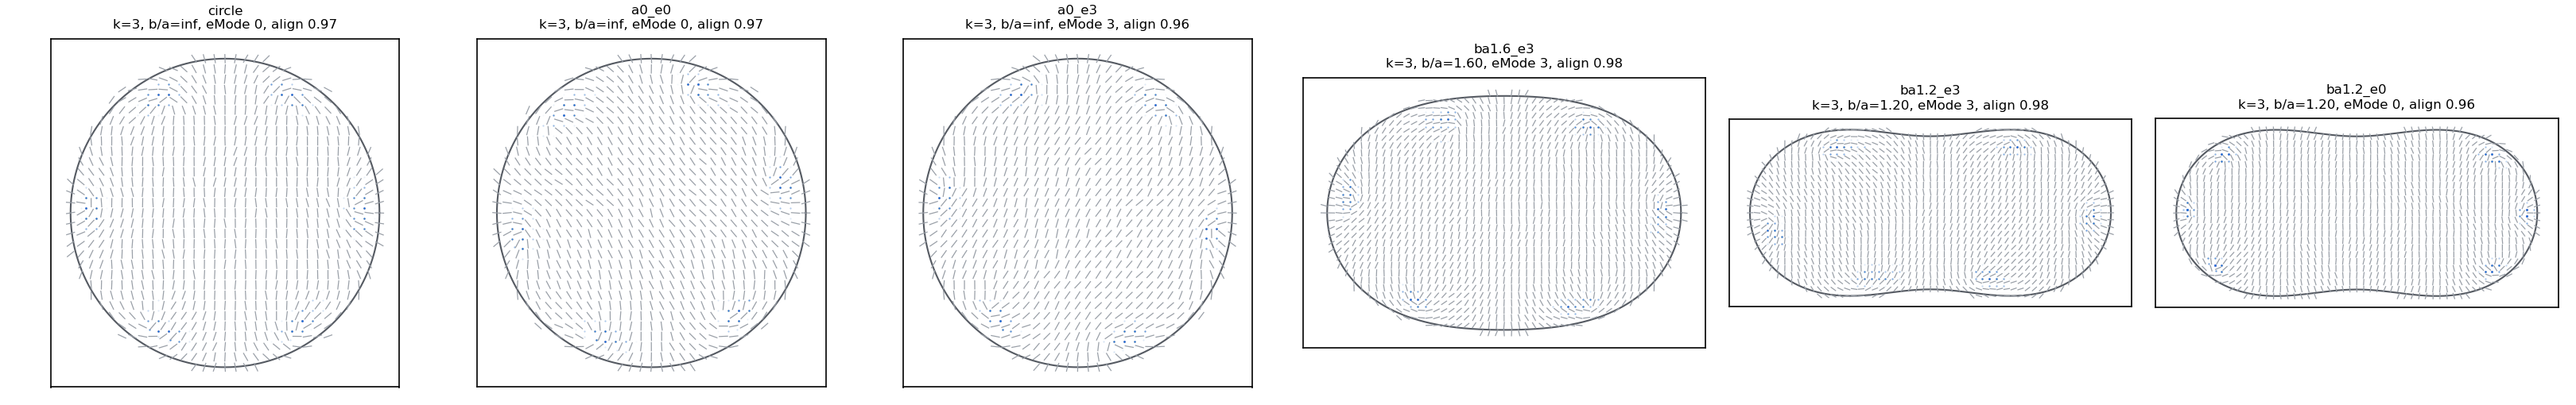
\includegraphics[width=\textwidth]{cassini_validation.png}
\caption{Passive validation of the Cassini wall ($k=3$): circle reference, $a=0$ with eMode 0 and 3, ovals $b/a=1.6$ and 1.2
with eMode 3, and $b/a=1.2$ with eMode 0.}\label{fig:cassval}
\end{figure}
\paragraph{Active length.} \SIcand
\begin{figure}[H]\centering
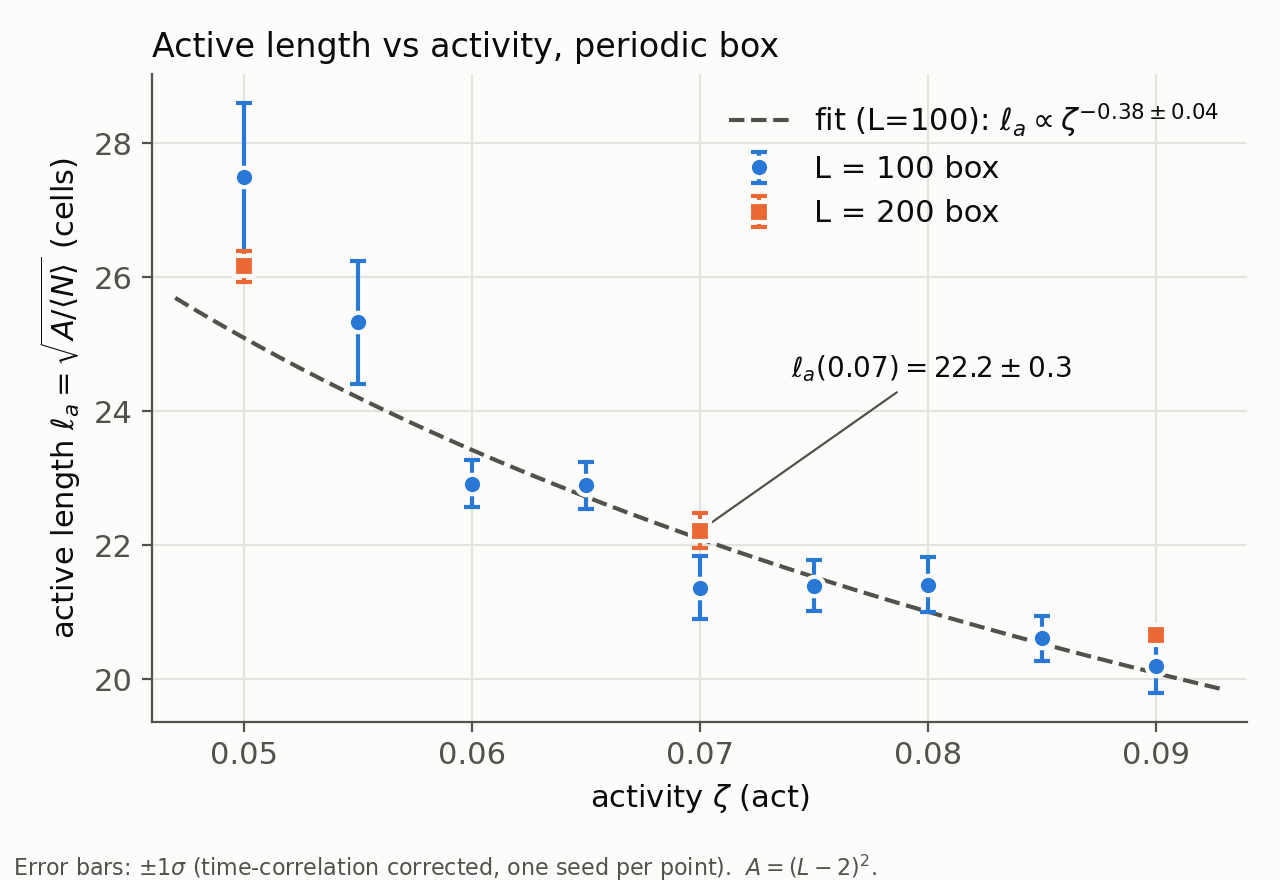
\includegraphics[width=0.75\textwidth]{active_length.png}
\caption{Active length against activity in periodic boxes of $100^2$ and $200^2$ cells, with a power-law fit.}\label{fig:la}
\end{figure}
\begin{table}[H]\centering\small
\caption{Active length (cells). $200^2$ values at 0.06 and 0.11: mean of two seeds (seed spread 1.2--1.5$\sigma$).}\label{tab:la}
\begin{adjustbox}{max width=\textwidth}
\begin{tabular}{lccccc}\toprule
$\zeta$ & 0.05 & 0.06 & 0.07 & 0.09 & 0.11\\\midrule
$\la$, $100^2$ & $27.5\pm1.1$ & $22.9\pm0.4$ & $21.4\pm0.5$ & $20.2\pm0.4$ & --\\
$\la$, $200^2$ & $26.2\pm0.2$ & $24.3\pm0.1$ & $\mathbf{22.2\pm0.3}$ & $20.7\pm0.1$ & $19.1\pm0.1$\\\bottomrule
\end{tabular}
\end{adjustbox}
\end{table}
No significant finite-size effect between the boxes (differences $-4.8\%$, $+4.0\%$, $+2.3\%$ at 0.05, 0.07, 0.09; 1.1--1.6$\sigma$).
$\la\propto\zeta^{-1/2}$ up to $\zeta\approx0.08$ ($\alpha=0.485\pm0.031$), flattening above (full range $\alpha=0.39$).
The exponent is not part of the paper (it is covered by published work); only $\la(0.07)$ enters, as the length unit.
\paragraph{Compressibility.} Density standard deviation 6.1 $\to$ 9.8 (Poisson 4.47) and rms Mach number 0.66 $\to$ 1.0
($c_s=1$) from $\zeta=0.05$ to 0.09 in periodic boxes; no threshold. In cavities the vortex adds a radial stratification
(Sec.~\ref{sec:activity}).

\section{Charge, layer and bulk observables}\label{sec:m-charge}
% ======================================================================
% Methods: defect statistics, charge profiles and edge/bulk criteria
% Generated from the analysis scripts in runs/cavity and runs/cassini.
% All facts checked against the code (2026-10-05). Where code and
% RESEARCH.md disagree, the code is followed and a NOTE is left.
% ======================================================================

\subsection{Defect data and charge audit}
\label{sec:methods-audit}

\paragraph{Raw data.}
All defect analyses start from the solver's defect file \texttt{defects.dat}
(read transparently from \texttt{defects.dat.gz} when the run was compressed).
Each frame consists of a header line with two numbers, the time $t$ and the number
$n$ of defects, followed by $n$ lines with four columns: the position $(x,y)$ in
cell units, the topological charge $q$ and the orientation angle $\psi$ of the defect.
The tracker only reports clusters with $|q|\simeq 1/2$; the charge column holds
values within $10^{-2}$ of $\pm 1/2$ (in a typical run $\approx 0.1\%$ of entries
differ from $\pm0.5$ by $10^{-3}$--$5\times10^{-3}$). Defect frames are written every
\texttt{defectsOut} $=20$ MPCD steps, i.e.\ every $\Delta t_{\rm f}=2$ time units
($\delta t = 0.1$); the main circle sweep records $10^4$ time units of production
($5001$ frames) after a $10^4$-step warm-up that is not written.
Non-numeric lines (the banner and column headers) are skipped; a truncated final frame
(fewer than $n$ defect lines) is discarded (\texttt{defect\_audit.read\_frames}).
Positions are shifted to the cavity centre $\mathbf{Q}$ given in \texttt{input.json}.

\paragraph{Transient.}
Unless stated otherwise every script discards the first $20\%$ of the recorded frames
(\texttt{--tfrac 0.2}), i.e.\ $2000$ time units in the main sweep, and uses the remaining
$\approx 4000$ frames. \texttt{defect\_spatial.load} and all scripts built on it drop
the first $\lfloor 0.2\,N_{\rm f}\rfloor$ frames by count; \texttt{layer\_analysis.load}
drops frames with $t < t_{\min}+0.2\,(t_{\max}-t_{\min})$, which is equivalent for
uniform sampling. \texttt{circulation.py} uses all production frames (\texttt{--tmin 0};
the warm-up is not in the files).

\paragraph{Charge audit (\texttt{defect\_audit.py}).}
For imposed winding $k$ (sign $\sigma_k=\mathrm{sgn}\,k$) every frame is checked for
topological consistency using only the signs of the tracked charges. With
$N_{\rm same}$ the number of defects with the sign of $k$ and $N_{\rm opp}$ the number of the
opposite sign,
\begin{equation}
  q_{\rm tot} = \tfrac12\,\sigma_k\,(N_{\rm same}-N_{\rm opp}),
\end{equation}
and the frame is classified by three flags:
\begin{itemize}
  \item \emph{net charge}: $|q_{\rm tot}-k|<1/4$ (charge conservation, total charge $=k$);
  \item \emph{imposed}: $N_{\rm same}\ge 2|k|$ (all boundary-imposed $\pm1/2$ present);
  \item \emph{pairs}: $N_{\rm same}-2|k| = N_{\rm opp}$ (the dynamical defects,
        $N_{\rm dyn}=N_{\rm same}+N_{\rm opp}-2|k|$, come in $\pm1/2$ pairs).
\end{itemize}
For $\pm1/2$ charges the last flag is equivalent to the first; they are reported
separately because the failure mode is diagnostic: a frame with $N_{\rm same}<2|k|$
has lost wall defects (``missing imposed''), a frame that passes ``imposed'' but not
``pairs'' has a missed, spurious or split pair member (``unpaired''). Per run we report
the fraction of frames with $q_{\rm tot}=k$, the fractions ``missing imposed'' and
``unpaired'', the fraction with odd $N_{\rm dyn}$, $\langle q_{\rm tot}\rangle$ and the mean
number of dynamically created pairs $\langle N_{\rm pairs}\rangle=\langle N_{\rm opp}\rangle$.
The audit needs no geometry and therefore applies unchanged to ovals and ellipses.
In passive validation runs it is satisfied in $100\%$ of frames; in the active fixed-$R$ scans
at $\zeta=0.07$ it holds in $\ge98\%$ of frames. The anchoring itself fails (audit
$\le 30\%$) for imposed linear densities $\rho\gtrsim0.25$, which bounds the parameter
space analysed ($\rho\le 0.15$).
% NOTE: the audit uses sign(q) only; quantities built on the raw charge column (Q(c), site-rule q_b)
% carry the small (~1e-3) deviations of individual charges from +-1/2 (see the P1 note below).

\subsection{Spatial distributions}
\label{sec:methods-spatial}

\paragraph{Time-averaged maps (\texttt{defect\_spatial.py}).}
Positions of $+1/2$ and $-1/2$ defects from all retained frames are binned on a square
grid of $0.5\times0.5$ cells covering $[-R-0.5,R+0.5]^2$; counts are divided by the number of
frames and the bin area, giving the mean number density $n_\pm(\mathbf{x})$ (defects per
cell$^2$ per frame). The maps are shown on a logarithmic scale spanning three decades.

\paragraph{Radial densities in circles.}
With $s=R-r$ the distance from the wall, defects are binned in $s$ with width
$\Delta s=0.25$ (\texttt{--sbin}); the counts are divided by the exact annulus area
$\pi(r_{\rm out}^2-r_{\rm in}^2)$ and by the number of frames, giving $n_\pm(s)$.

\paragraph{Defect speeds.}
For each pair of consecutive frames and each sign, every defect is matched to the nearest
same-sign defect of the next frame; the match is accepted if the distance is below
$r_{\rm link}=3$ cells, and the speed is the displacement divided by $\Delta t_{\rm f}$. Speeds are
binned in $s$ (same bins as $n_\pm$) and averaged over bins with at least $20$ samples.
This matching is nearest-neighbour (not one-to-one).
% NOTE: with Delta t_f = 2 and bulk +1/2 speeds ~0.8-1 cells/time, r_link = 3 rejects the fastest
% steps (RESEARCH 2026-10-01 18:20: ~90% of track breaks at r_link = 3 were genuine 3-6 cell jumps), so
% the bulk speed profile is biased low; the tracking used for the mobility criterion uses r_link = 8.
Layer $+1/2$ defects move at $0.2$--$0.35$ cells per time unit, indistinguishable from passive
pinned defects ($\approx0.3$, the tracker's positional jitter), whereas bulk $+1/2$ move at
$0.8$--$1.0$.

\paragraph{Angular sites in circles.}
As a first count of pinned wall defects, the polar angles of all $+1/2$ with $s<4.2$ are
histogrammed in $360$ bins, smoothed periodically with a Gaussian of width $2$ bins
(13-tap kernel) and the number of runs (contiguous intervals) of bins above $15\%$ of the
maximum is counted (\texttt{defect\_spatial.layer\_sites}). This circle-specific count is
superseded by the shape-independent site rule of Sec.~\ref{sec:methods-sites}.

\paragraph{Profiles along Cassini and ellipse levels (\texttt{lobe\_profiles.py}).}
For Cassini ovals with foci at $(\pm a,0)$ and wall $d_1d_2=b^2$ we use the level coordinate
\begin{equation}
  c(\mathbf{x}) = \sqrt{d_1 d_2},\qquad d_{1,2}=|\mathbf{x}\mp a\hat{\mathbf{e}}_x| ,
\end{equation}
so that $c=0$ at the foci, $c=a$ on the lemniscate (for $c<a$ the level consists of two
separate lobe ovals) and $c=b$ on the wall; for $a=0$ (circles) $c=r$. For ellipses with
semi-axes $\varepsilon B$ (along $x$) and $B$ (along $y$) the levels are scaled copies of the
wall,
\begin{equation}
  c(\mathbf{x}) = \sqrt{(x/\varepsilon)^2+y^2},\qquad c=b\equiv B \text{ on the wall},
\end{equation}
with $\varepsilon$ and $B$ read from the wall parameters ($\varepsilon = a^{-1}_x/a^{-1}_y$,
$B=R\,a^{-1}_y$ for \texttt{aInv} $=(a^{-1}_x,a^{-1}_y,\cdot)$).
The interval $c\in[0,b]$ is divided into $N_{\rm sh}$ shells uniform in $c/b$
($N_{\rm sh}=200$ for all quantitative results, i.e.\ $\Delta(c/b)=0.005$; the plotting default is
60). Shell areas are exact for ellipses, $A_j=\pi\varepsilon(c_{j+1}^2-c_j^2)$, and for
Cassini ovals are obtained by counting the points of a $0.1$-cell grid whose $c$ falls in the
shell. Densities are $n_\pm(c)=$ (defects in the shell per frame)$/A_j$. Profiles per lobe
are obtained by restricting to $x<0$ or $x>0$ (meaningful for $c<a$ only). For Cassini ovals
the physical width of a shell varies along the level ($\propto 1/|\nabla c|$, widest at the
neck), which smears a thin wall layer; conclusions were therefore cross-checked against
profiles in the true wall distance (Sec.~\ref{sec:methods-walldist}).

\subsection{Accumulated charge and level coordinates}
\label{sec:methods-Q}

\paragraph{Accumulated charge $Q(c)$.}
The central observable is the mean net charge enclosed by a level,
\begin{equation}
  Q(c_j) = \Big\langle \sum_{i:\,c(\mathbf{x}_i)<c_j} q_i \Big\rangle_t ,
\end{equation}
computed as the cumulative sum over shells of the charge histogram (weights $q_i$, the raw
charge column) divided by the number of frames, and evaluated at the \emph{outer} shell
edges $c_j/b = j/N_{\rm sh}$ (\texttt{lobe\_profiles.profile}). In circles $Q(r)$ is the
charge inside radius $r$. By construction $Q(b)=k$ (up to defects reported outside the
wall, which are not counted). Per-lobe charges $Q_{L,R}(c)$ use $x<0$ or $x>0$.
For circles, $Q(r)$ shows a negative dip towards the centre ($-1/2$ excess), a plateau
at $+1$ just inside the wall, and a jump to $k$ in the last few percent of $R$ (the layer).

\paragraph{Fixed-distance enclosed charge $Q(s)$.}
As a cut-free alternative in general shapes, \texttt{cassini\_charge.py} reports the mean
net charge of defects farther than $s$ from the wall, for $s\in\{1,2,3,4,5,6,8,10\}$
cells, with $s$ the first-order wall distance of Sec.~\ref{sec:methods-walldist}.
In circles at $\zeta=0.07$ this is flat ($Q\approx1.0$) for $s=3$--$5$; in elongated ovals it
falls steadily without a plateau, so a single ``bulk'' value at fixed $s$ is cut-dependent there.

\paragraph{Wall distance in general shapes.}
\label{sec:methods-walldist}
For the Cassini family ($a=0$: circle) the wall function is $W=d_1d_2-b^2$, and the distance
from the wall and the outward normal angle are taken to first order,
\begin{equation}
  s(\mathbf{x}) = -\frac{W}{|\nabla W|},\qquad
  \nabla W = \Big(\tfrac{d_2}{d_1}(x-a)+\tfrac{d_1}{d_2}(x+a),\;
  \big(\tfrac{d_2}{d_1}+\tfrac{d_1}{d_2}\big)y\Big),\qquad
  \phi_n = \operatorname{atan2}(\partial_yW,\partial_xW)
\end{equation}
(\texttt{edge\_criteria.wall}, \texttt{cassini\_charge.wall\_distance}).
% NOTE: s = -W/|grad W| is exact only at the wall. For a circle it gives s = (R^2 - r^2)/(2r)
% = (R - r)(R + r)/(2r), not R - r: at R = 31.8 the cut s < 6 corresponds to a true distance of
% ~5.4 cells, and s diverges at the centre. Ellipse runs (shape 0, aInv_x != aInv_y) are treated as
% circles of radius R by these two functions (only cassiniA / shape 1 is read).
For the mean wall distance along a level curve (Sec.~\ref{sec:methods-dstar}) the exact
Euclidean distance to a polygon of $4000$ wall points is used, the wall being
$r^2(\theta)=a^2\cos2\theta+\sqrt{b^4-a^4\sin^2 2\theta}$ (single oval, $b>a$).

\subsection{Bulk charge from the shape of $Q(c)$: knee, $d^*$ and $f^*$}
\label{sec:methods-knee}

\paragraph{Knee of $Q(c)$ (\texttt{charge\_knee.py}).}
The bulk charge is read from the plateau of $Q$ just inside the wall, located as the
``knee'', i.e.\ the outermost point where $Q$ is clearly flatter than on both sides.
With $x_j=c_j/b$ the outer shell edges ($N_{\rm sh}=200$):
\begin{enumerate}
  \item \emph{Smoothing.} $Q$ is padded with $9$ copies of its first and last values and
        convolved with a $9$-bin box kernel, $\tilde Q = Q * \mathbf{1}_9/9$, i.e.\ smoothed over
        $0.045$ in $c/b$. The slope is $S=\mathrm{d}\tilde Q/\mathrm{d}x$ (centred finite differences,
        \texttt{numpy.gradient}).
  \item \emph{Search window.} From $i_0+2$ (with $i_0=\arg\min\tilde Q$, the $-1/2$ core; at least
        index 3) up to the index of $x=0.985$ minus 3.
  \item \emph{Candidates.} Local minima of $S$ ($S_i\le S_{i\pm1}$) that satisfy all of
        \begin{align}
          S_i &\le 0.7\, \max_{x_i-0.12\le x_j< x_i} S_j &&\text{(flatter than the inner side)},\\
          S_i &\le 0.2\, \max_{x_i< x_j\le 0.985} S_j &&\text{(flatter than the jump to the wall)},\\
          \tilde Q_i - \tilde Q(x_i-0.2) &\ge 0.5 &&\text{(a plateau is reached by a rise)} .
        \end{align}
  \item \emph{Selection.} Among the candidates the one closest to the wall (largest $x_i$) is the knee.
\end{enumerate}
The bulk charge is $Q_{\rm knee}=\tilde Q(x_{\rm knee})$, the layer charge $k-Q_{\rm knee}$; if no
candidate exists the run has \emph{no knee} (no layer/bulk split). The plateau contrast
$\max_{\rm wall\,side}S/S_{\rm knee}$ is also recorded. The rise condition excludes noise minima in
a flat interior; the $0.985$ limit excludes the final jump onto the wall.
The smoothing width was changed from $5$ to $9$ bins after the main-sweep analysis: with $5$ bins
the finder picked up the flat shoulders of the cell-quantised layer steps (width $\approx0.02$ in
$c/b$), e.g.\ a spurious knee at $Q\approx1.9$ for $k=5$, $R\approx0.8$--$0.9\,\la$ whose true plateau is
at $+1.0$; $9$ bins ($0.045$) removes these steps but preserves a genuine plateau
($\approx0.1$ wide). All runs were re-analysed with $9$ bins; the established cases were unchanged.
The same function is applied to ovals and ellipses in their own level coordinate.

\paragraph{Mirror runs ($k<0$): peak of $Q$.}
For negative winding $Q$ rises to a positive maximum and then plunges to $-|k|$ at the wall, so the
bulk charge is taken as the maximum of the smoothed $\tilde Q$ (same $9$-bin smoothing) over
$x<0.97$ (\texttt{criteria\_all.py}). It is accepted as a plateau only if (i) the band of $x<0.97$
where $\tilde Q>\tilde Q_{\max}-0.1$ is at least $0.04$ wide in $r/R$, (ii) the steepest
$|\mathrm{d}\tilde Q/\mathrm{d}x|$ between the peak and the wall is at least $5\times$ the mean
$|\mathrm{d}\tilde Q/\mathrm{d}x|$ over the band, and (iii) $\tilde Q_{\max}>0.05$. The earlier survey
script \texttt{mirror\_analysis.py} reports the unsmoothed peak of $Q$ for $x<0.97$, its position and
the width of the band within $0.1$ of it, together with the mean numbers of $\pm1/2$ within $s<3$
(wall) and $s\ge3$ (bulk) per frame.

\paragraph{Layer depth $d^*$ (\texttt{layer\_depth.py}).}
\label{sec:methods-dstar}
The level $c^*$ where $Q$ crosses $+1$ on its way to $k$ is located by scanning inward from the
wall: with $i$ the outermost shell edge where $Q<1$,
$c^*/b = x_i + (1-Q_i)(x_{i+1}-x_i)/(Q_{i+1}-Q_i)$ (linear interpolation; unsmoothed $Q$).
The layer depth is the mean wall distance along the level $c=c^*$. In circles $d^*=R-c^*$
(as used in \texttt{main\_sweep\_analysis.py}). For ovals the level is sampled on a square grid of
spacing $h=0.15$: all grid points with $|c(\mathbf{x})-c^*|<\tfrac12 h\max(1,\overline{|\partial_x c|})$
(median over nearby points) are retained and their exact distances to the wall polygon are averaged.
% NOTE: the docstring/RESEARCH call this an "arclength-weighted" mean. Grid points in a band of fixed
% width in c are weighted by 1/|grad c| per unit arclength (denser where levels are farther apart,
% i.e. at the neck), so the mean is arclength-weighted only where |grad c| is constant along the level
% (exactly so for circles).
$d^*$ is reported in cells, in units of $\la$ ($\la=22.21$) and relative to the cavity size.
A plateau width $w$ (the wall-distance difference between the inner and outer ends of the contiguous
band around $c^*$ with $|Q-1|<0.15$) is also computed, but is unreliable for ovals (it can become
negative when $Q$ merely passes through $1$) and is not used.

\paragraph{Layer area fraction $f^*$ and effective width (\texttt{layer\_area.py}).}
With $c^*$ as above,
\begin{equation}
  f^* = \frac{A(c^*<c<b)}{A(c<b)},\qquad w_{\rm eff}=\frac{A(c^*<c<b)}{P},
\end{equation}
with areas counted on a $0.1$-cell grid and $P$ the perimeter of the $4000$-point wall polygon.
In circles $f^*=1-(c^*/R)^2$ (\texttt{main\_sweep\_analysis.py}, \texttt{criteria\_all.py}).
$f^*=1/2$ (the ``layer'' as large as the region it encloses) is used as the bound beyond which the
outer region is not a layer: clean circles have $f^*\le0.32$. For a true layer $f^*\propto$
width$/$size decreases with cavity size, whereas a charge distribution spread through the cavity
gives a size-independent $f^*$; the size scaling of $f^*$ thus distinguishes the two.
% NOTE: layer_area.py / layer_depth.py read the geometry with lobe_profiles.geometry, which ignores
% the ellipse parameters (a = 0, b = R). Because ellipse levels are self-similar, f* = 1 - (c*/b)^2 is
% still correct for ellipses, but w_eff and d* would be computed for a circle of radius R; only f* is
% quoted for ellipses. layer_area.py has no guard for runs where Q never drops below 1.
In mirror runs the $+1$ crossing is taken from the centre outward (first $x<0.97$ with $Q\ge1$).

\subsection{Edge/bulk classification of individual defects}
\label{sec:methods-criteria}\label{sec:edge}

All criteria below assign each defect of a frame to the wall layer (``edge'') or to the bulk; the bulk
charge is the mean net charge of bulk defects, $q_b=\langle\sum_{i\in\rm bulk}q_i\rangle_t$, and
$P_1$ is the fraction of frames with $q_b=+1$ (tested as $|q_b-1|<1/4$ unless noted).
In the per-defect rules (site, density, mobility, tilt) only defects of the sign of $k$ (the wall-imposed sign) are
ever assigned to the edge; the charge-profile criteria (knee, fixed cut, $q_{\rm dens}$) assign everything outside a level to the edge.

\paragraph{Fixed geometric cuts.}
(i) $q_{\rm fixed}=Q(r=\tfrac{11}{12}R)$, linearly interpolated in the $200$-shell $Q(r)$
(\texttt{criteria\_all.py}). (ii) In \texttt{circulation.py} bulk defects are those with
$r<R-2.5$; $q_b(t)=\tfrac12\sum_{\rm bulk}\mathrm{sgn}\,q_i$. Fixed cuts fail when the layer thickness
does not scale with $R$: below $\sim1\,\la$ the layer is thicker than $R/12$ (then $q_{\rm fixed}\gg1$),
and for $k<0$ at $R\lesssim1.5\,\la$ it is strongly negative; they are reported only for comparison.
% NOTE: RESEARCH (2026-09-30) notes that the fixed --wall 2.5 in circulation.py underestimates the layer.

\paragraph{Passive edge $d_p$ (\texttt{layer\_analysis.py}).}
The layer is taken from the passive run with the same $(R,k)$ (located by the same \texttt{rho}/\texttt{k}
path, seed \texttt{s01}): $d_p$ is the $95$th percentile of $s=R-r$ over all same-sign defects of the passive
run (after the 20\% transient), and a layer is said to exist if at least half of them lie within $5$ cells
(\texttt{--layer-max}) of the wall. Bulk: $s>d_p$. This cut was abandoned: the passive layer shrinks
from $8.3$ to $2.3$ cells with $k$ and is thinner than the active one at $k\gtrsim6$ (and too wide at $k=2$),
giving $q_b$ from $0.44$ to $1.20$ in a set where the density cut gives $1.00\pm0.02$ for every $k$.

\paragraph{Density-minimum edge $d_\rho$.}
Two implementations are used.
\begin{itemize}
  \item \texttt{layer\_analysis.density\_edge}: the radial density of same-sign defects is computed in
        bins of $0.5$ cells in $s\in[0,\min(R,12)]$ (per annulus area and frame). The wall peak is the
        maximum among bins with centre $s<3$; $d_\rho$ is the bin centre of the minimum of the $3$-bin box-smoothed
        density over bins with $s_{\rm peak}<s\le\min(8,R/2)$. Bulk: $s>d_\rho$; layer: same-sign defects with
        $s\le d_\rho$. From the layer we also record the occupancy $N_L(t)$, its relative fluctuation
        $\mathrm{std}/\mathrm{mean}$ and the radial width (standard deviation of $s$ in the layer).
  \item \texttt{criteria\_all.py} ($q_{\rm dens}$), on the $200$-shell profile in $x=r/R$: the wall-sign density
        $n_{\sigma_k}$ is smoothed with a $5$-bin box ($\Delta x=0.025$); the wall peak is its maximum for
        $x>1-6/R$ (within $6$ cells of the wall); the gap is the minimum of the smoothed density between
        $x_{\rm lo}=\max(1-10/R,\,0.3)$ (within $10$ cells of the wall) and the peak, required to lie at
        least $2$ bins inside it. Then $q_{\rm dens}=Q(x_{\min})$ (charge inside the minimum, original signs).
        Undefined if the peak is not more than $2$ bins outside $x_{\rm lo}$.
\end{itemize}
In circles at $\zeta=0.07$ the $+1/2$ density has a sharp wall peak at $s\approx1$--$2$, a gap at
$s\approx3$--$5$ about $5\times$ below the bulk plateau, and the speed step sits at the same $s$, so
$d_\rho\approx4$ cells. The gap does not scale with $\la$ (layer width is set in cells, bulk density
$\propto\la^{-2}$): it is shallow at $\zeta=0.06$ and almost absent at $0.11$, where the split becomes
ill-defined. The density criterion gives $q_b\to0$ in very small cavities ($R\lesssim0.6$--$0.8\,\la$,
no bulk defects).

\paragraph{Pinned-site rule (\texttt{edge\_sites.classify}).}
\label{sec:methods-sites}
Wall defects are stationary, so they leave sharp spots in the time-averaged density while mobile bulk
defects average out.
\begin{enumerate}
  \item \emph{Sites.} The $+1/2$ positions of all retained frames are binned on a $0.5$-cell grid,
        normalised to defects per cell$^2$ per frame and smoothed with a Gaussian of
        $\sigma=1$ cell. Sites are local maxima (equal to the maximum in a
        $9\times9$-bin, i.e.\ $4.5\times4.5$-cell, window; window size $2\,\mathrm{round}(2\sigma/0.5)+1$)
        that exceed $0.02$ defects per cell$^2$ per frame. No radial cut or circle geometry is used.
  \item \emph{Capture radius.} For every $+1/2$ occurrence the distance to the nearest site is computed;
        its histogram (bins of $0.25$ cells on $[0,12]$) is smoothed with a $5$-bin box and
        $d_{\rm site}$ is the position of its minimum between $1.5$ and $8$ cells (fallback $3$ cells).
        A fixed $d_{\rm site}=2$--$3$ is too tight (in a passive $k=5$ run it captures only $7.8$--$9.6$
        of $10$ pinned defects).
  \item \emph{Cap.} $d_{\rm site}$ is capped at $0.4\times$ the median nearest-neighbour distance
        between sites (\texttt{--dfrac 0.4}). Without the cap, when the bulk $+1/2$ ring presses against
        the layer (no dip in the histogram, e.g.\ $\zeta=0.11$, $k\ge7$) the minimum runs to the $8$-cell
        window edge and the rule captures bulk defects ($q_b\approx-0.5$).
        % NOTE: RESEARCH says the cap "never binds" at zeta = 0.07 (max |Delta q_b| = 0), but also
        % that the uncapped d_site ~ half the site spacing in the R-scan; 0.4 x spacing < 0.5 x spacing, so
        % the cap may bind there without changing q_b. The code records a 'capped' flag per run.
  \item \emph{Classification.} A $+1/2$ within $d_{\rm site}$ of a site is edge; all other defects
        (and every $-1/2$) are bulk. Per frame $q_b(t)=\sum_{\rm bulk}q_i$ and the edge occupancy $N_E(t)$.
\end{enumerate}
Reported per run: number of sites (compare with $2k-2$), mean wall distance of the sites, $d_{\rm site}$,
$\langle N_E\rangle$, $\langle q_b\rangle$ with a block error ($10$ consecutive blocks, standard error of
the block means), $P_1$, and the fraction of $+1/2$ occurrences classified identically by the site rule
and by a density cut at $s=4.2$ (circles: $96$--$99.7\%$ at $\zeta=0.07$).
% NOTE: in edge_sites.classify P1 is computed as np.isclose(q_b, 1) on the raw charge column, whose
% entries differ from 0.5 by up to 5e-3 in ~0.1% of defects; frames containing such a defect fail the
% test, so P1(site) is biased low by roughly the fraction of such frames (percent level). Other P1's
% use sign(q) and |q_b - 1| < 1/4.
For mirror runs ($k<0$) the frames are sign-flipped before classification, so the sites are those of the
wall $-1/2$, and $q_{\rm site}=\sigma_k\,q_b$ is returned in the original charges (\texttt{criteria\_all.py}).
For Cassini ovals the bulk charge is also split into left and right halves ($x<0$, $x>0$)
(\texttt{cassini\_charge.py}). Limitations: in passive runs at $k=2,3$ the pinned defects sit away from the
wall (the rule finds pinned, not wall, defects; $q_b=0$ is still correct), and at $\zeta=0.05$, $k=9,10$
(flow reversals) spurious interior maxima give $16$--$27$ sites; such runs are flagged.

\paragraph{Linking defects into tracks.}
Three linkers are used.
\begin{itemize}
  \item \texttt{edge\_criteria.link} ($+1/2$ only): consecutive frames are matched by an optimal
        one-to-one assignment (Hungarian algorithm, cost = distance, pairs beyond $r_{\rm link}$ forbidden);
        unmatched defects start new tracks; no gap closing.
        $r_{\rm link}=8$ cells is used for all reported criteria (the command-line default is $3$).
        With $\Delta t_{\rm f}=2$ and cell-quantised positions, $r_{\rm link}=3$ breaks most bulk tracks
        (median track length one frame); $r_{\rm link}=8$ reduces the number of tracks $\sim9\times$ and
        $>90\%$ of track starts/ends are then paired with an opposite-sign start/end.
  \item \texttt{layer\_analysis.link} (both signs): optimal assignment per frame with gap closing:
        a track may miss up to $3$ frames, the admissible jump grows as $r_{\rm link}\sqrt{g}$ for a gap of $g$
        frames, opposite signs are never linked, and a penalty $0.5(g-1)$ is added to the cost to prefer
        continuing tracks seen in the last frame ($r_{\rm link}=3$; runs with $\Delta t_{\rm f}>2.5$ are flagged as
        unreliable for linking).
  \item \texttt{defect\_spatial} speeds: nearest neighbour, see Sec.~\ref{sec:methods-spatial}.
\end{itemize}

\paragraph{Mobility criterion (\texttt{edge\_criteria.py}).}
For every $+1/2$ occurrence at frame $n$ on track $j$, the net displacement over a window $\tau$,
\begin{equation}
  D = |\mathbf{r}_j(n+h)-\mathbf{r}_j(n-h)|,\qquad h=\max\!\big(1,\mathrm{round}(\tau/2\Delta t_{\rm f})\big),
\end{equation}
with $\tau=20$ time units ($h=5$ frames). Occurrences whose track does not exist at both $n-h$ and $n+h$,
and frames within $h$ of either end of the series, are skipped. Wall defects in circles have a median
$D$ of $1.0$--$1.4$ cells against $10$--$11$ for bulk $+1/2$.
In \texttt{criteria\_all.py} a defect is ``slow'' (edge) if $D<5$ cells \emph{and} $s<6$ (first-order
wall distance). The bulk charge is then obtained from the total charge,
\begin{equation}
  q_{\rm slow} = k - \tfrac12\,\frac{N_{\rm slow}}{N_{\rm f}'},
\end{equation}
with $N_{\rm slow}$ the number of slow occurrences and $N_{\rm f}'=N_{\rm f}-2h$ the number of frames
used. Normalising by frames (not by the number of tracked $+1/2$) avoids a bias towards the edge,
because bulk tracks break more often than wall tracks.
% NOTE: occurrences skipped because their track breaks inside the window are not counted as slow,
% so N_slow/N_f' is a lower bound on the edge count (q_slow biased high) when wall tracks break;
% this assumes total charge k (audit) rather than counting bulk defects directly.
For mirror runs the sign of all charges is flipped before linking so that the wall $-1/2$ are followed,
and $q_{\rm slow}=k+\tfrac12 N_{\rm slow}/N_{\rm f}'$.

\paragraph{Tilt criterion.}
The orientation of a wall $+1/2$ relative to the local outward wall normal is
$\Delta=\mathrm{wrap}_{(-\pi,\pi]}(\psi-\phi_n)$, with $\psi$ the angle column of \texttt{defects.dat} and
$\phi_n$ the normal angle of Sec.~\ref{sec:methods-walldist}. In circles wall $+1/2$ are tilted by
$|\Delta|\approx1.1$~rad ($\approx63^\circ$) with the sign of the vortex sense, nearly independent of $k$,
while bulk $+1/2$ cluster near $|\Delta|\approx\pi-0.5\approx2.4$~rad. The combined criterion
(``slow and tilted'', $+k$ only) counts an occurrence as edge if $D<5$, $s<6$ and $|\Delta|<1.8$~rad,
$q_{\rm tilt}=k-\tfrac12 N_{\rm tilt}/N_{\rm f}'$. Only an upper cut is used because the wall tilt
decreases from $\approx1.1$~rad at $\rho=0.06$ to $\approx0.85$~rad at $\rho=0.15$ and broadens.
% NOTE: an earlier version (RESEARCH 2026-10-01 17:20) used a window 0.5 < |Delta| < 1.8; criteria_all.py
% has no lower cut.
Even so, slow-and-tilted overcounts the bulk ($q_b\approx1.3$--$1.6$) at high $\rho$, where the wall tilt
falls to $30$--$40^\circ$.

\paragraph{Calibration against the site rule.}
\texttt{edge\_criteria.py} also determines, per run, the single threshold on $D$ (scanned over $200$ values
in $[0.5,30]$) and on $|\Delta|$ (over $[0.05,\pi]$) that maximises the agreement (fraction of $+1/2$
occurrences classified identically) with the site rule, and the agreement of the combination. In circles
with $R\le2.15\,\la$ each criterion alone agrees with the site rule on $97$--$99\%$ of occurrences
($0.89$ at $2.87\,\la$).

\paragraph{Summary of criteria per run (\texttt{criteria\_all.py}).}
For every circle run of the main sweep with $\rho=|k|/(\pi R)\le0.151$, both windings, the script computes
$q_{\rm knee}$ (knee for $k>0$, peak-plateau for $k<0$) and its position, $q_{\rm fixed}$, $q_{\rm site}$
and the number of sites, $q_{\rm dens}$ and $r_{\rm dens}$, $q_{\rm slow}$, $q_{\rm tilt}$ ($k>0$), the
$+1$ crossing $r^*/R$ and $f^*=1-(r^*/R)^2$. All inputs use $200$ shells and the 20\% transient.
The knee is the primary criterion (defined and $\approx1$ from $\sim0.6$ to $\sim2.4\,\la$ for $+k$); the
density minimum and mobility are cross-checks.

\paragraph{Layer occupancy and docking (\texttt{layer\_analysis.py}).}
Using $d_\rho$ (or $d_p$ when a passive reference exists), a docking event is a step of a same-sign track
from $s>d$ to $s\le d$, undocking the reverse; rates are events per unit time. The circulation time before
docking is the time a docking track spent in the zone $d<s\le d+2$ immediately before. In the gap test, the
angular gaps between the other layer defects at the docking frame are computed and we record whether the
docking defect enters the largest gap, compared with the random expectation $\langle 1/n_{\rm gaps}\rangle$.
The azimuthal speed $|\Delta\theta|\,\bar r/\Delta t$ of same-sign defects is binned in $2$-cell bins of $s$
(steps spanning at most 2 frames).

\subsection{Pair correlations}
\label{sec:methods-gr}\label{sec:m-gr}

\paragraph{Lag-referenced $g_{ab}(r)$.}
In the inhomogeneous cavity the pair-distance histogram is normalised by a reference with the same one-body
density and no correlations: pairs between frame $i$ and frame $i+N_{\rm f}/2$ (cyclic), which are
decorrelated (\texttt{defect\_spatial.rdf}). For $ab\in\{++,--,+-\}$, $g_{ab}(r)$ is the ratio of the
within-frame histogram (bins of $1$ cell up to $2R$) to the cross-frame one, the latter rescaled per frame by
$\tfrac12N_a(N_a-1)/(N_aN_a')$ (same sign) or $N_aN_b/(N_aN_b')$ (opposite signs) to count pairs like the
within-frame histogram; bins with reference count $\le5$ are left blank. It is computed for all defects and
for bulk defects only ($r<R-4.2$). For static layer defects the reference contains effective self-pairs
(the passive $g$ shows the site lattice), so this estimator is meaningful only for mobile (bulk) defects.

\paragraph{Same-ring angular correlation $g_{ab}(s,\Delta\phi)$.}
The cavity is divided into rings of width $1$ in $s$; for each ring and frame, the angular separations
$\Delta\phi\in[0,\pi]$ of all pairs in the same ring are histogrammed in $90$ bins and divided by the uniform
expectation (pairs$\times\Delta\phi_{\rm bin}/\pi$); rings with fewer than $30$ pairs are blank. This needs only
within-frame pairs and no model of the radial profile; it resolves the layer lattice (peaks at
$\Delta\phi=2\pi m/(2k-2)$) but same-ring bulk pairs are too rare.

\paragraph{Ring-resolved $g_{ab}(r\,|\,s)$.}
For reference defects of type $a$ in ring $s$ (width $1$) and partners of type $b$ anywhere in the cavity,
the within-frame distance histogram (bins of $1$ cell up to $2R$, self excluded) is divided by the expected
count for an uncorrelated partner distribution with the measured radial density,
\begin{equation}
  E_{ab}(r\,|\,s) = N^{\rm ref}_a(s)\;2\pi r\,\Delta r\;\big\langle n_b\big(R-|\mathbf{r}_0+r\hat{\mathbf{e}}_\theta|\big)\big\rangle_\theta ,
\end{equation}
where $\mathbf{r}_0$ is a point at the ring's centre radius, the angular average uses $720$ directions,
$n_b(s)$ is the measured radial density ($\Delta s=0.25$) and $n_b=0$ outside the wall. Bins are shown if
$E>3$ and the ring has at least $30$ references. Seed-pooled maps (\texttt{edge\_sites.py}) sum observed and
expected counts over the seeds of each $(k,R,\zeta)$ before dividing ($E>5$); zone curves sum over rings in
three zones (edge $s<4.2$, outer bulk $4.2<s<R/2$, centre $s>R/2$) and over all $k$ at equal $R$ ($E>20$), with
a Poisson error $g/\sqrt{O}$. The thin layer peak in $n_b$ produces an artefact at the largest $r$ (partner in
the far-side layer).
% NOTE: the zone pooling uses R/2 of the first (k, R) group for all groups, i.e. it assumes equal R.

\subsection{Circulation order parameters}
\label{sec:methods-circ}

The coarse-grained velocity field (\texttt{flowfield.dat}; each frame is the average over the output
interval, every $1000$ steps $=100$ time units in the main sweep) is read per cell (cell centres at
integer$+\tfrac12$). Over the cells with $0.5<r<R-1$ (\texttt{--rcut 1}) we compute per frame
\begin{equation}
  m(t) = \big\langle \mathbf{v}\cdot\hat{\boldsymbol\phi}\big\rangle_{\rm cells},\qquad
  u(t) = \big\langle |\mathbf{v}|\big\rangle_{\rm cells},
\end{equation}
and the dimensionless order parameters
\begin{equation}
  \Phi_{\rm persist} = \frac{|\langle m\rangle_t|}{\langle u\rangle_t},\qquad
  \Phi_{\rm inst} = \frac{\langle |m|\rangle_t}{\langle u\rangle_t}.
\end{equation}
$\Phi_{\rm persist}$ measures a persistent sense of rotation; $\Phi_{\rm inst}$ is insensitive to
reversals of the spontaneously chosen sense. $\Phi_{\rm persist}\approx\Phi_{\rm inst}$ indicates a steady vortex,
$\Phi_{\rm inst}\gg\Phi_{\rm persist}$ a reversing one (e.g.\ $0.16$ vs $0.71$ in one test seed). The raw
$|\langle m\rangle_t|$ and $\langle|m|\rangle_t$ are also reported. The same script computes the bulk charge with
the fixed cut $r<R-2.5$, $P_1$, the audit fractions, and $P_1$, $\langle q_b\rangle$ restricted to audit-passing
frames (a difference would indicate that the audit filter biases the result) (\texttt{circulation.py}).

\subsection{Aggregation over seeds}
\label{sec:methods-aggregate}

\begin{itemize}
  \item \emph{Within a run}: time averages over the retained frames. Statistical errors of $\langle q_b\rangle$
        and $P_1$ are block errors with $10$ consecutive blocks (standard deviation of block means$/\sqrt{10}$;
        \texttt{layer\_analysis} truncates to equal blocks, \texttt{edge\_sites} uses near-equal splits).
  \item \emph{Parameter sets}: runs in seed directories (\texttt{.../rho*/k*/sNN}) are grouped by their parent
        directory; set values are the mean over seeds and errors the standard error,
        $\mathrm{std}_{\rm ddof=1}/\sqrt{n_{\rm seeds}}$ (\texttt{circulation.py}).
  \item \emph{Criteria maps}: per $(\mathrm{sgn}\,k,\rho,|k|)$ the bulk charge of each criterion is the mean over the
        seeds for which it is defined; a point is marked undefined if no seed has it (e.g.\ no knee) and flagged if
        it is defined in fewer than $2/3$ of the seeds (\texttt{plots\_criteria.py}, from \texttt{criteria\_all.csv}).
  \item \emph{Profiles}: seed-averaged $n_\pm(c)$ and $Q(c)$ are arithmetic means of the per-seed profiles on the
        common shell grid. Pair correlations are pooled by summing observed and expected counts before dividing
        (Sec.~\ref{sec:methods-gr}).
  \item \emph{Main-sweep table} (\texttt{main\_sweep\_analysis.py}): one row per run with $R$, $k$, $\rho=|k|/(\pi R)$,
        seed, $\zeta$, number of frames, $Q_{\rm knee}$, $c_{\rm knee}$ and contrast, $c^*/R$, $d^*=R(1-c^*/R)$,
        $f^*=1-(c^*/R)^2$, number of sites, $q_{\rm site}$, $P_1^{\rm site}$, and the wall Fourier quantities
        ($m^*$, $S(m^*)$, $f_{\rm static}$, $N_{\rm wall}$ from \texttt{wall\_fourier.py}, $+1/2$ within $4$ cells of
        the wall). The analysis is restartable (runs already in the table are skipped).
\end{itemize}
Lengths are normalised by the active length measured in periodic boxes at the same activity,
$\la(\zeta=0.07)=22.2\pm0.3$ (value $22.21$ used in the scripts), and densities by $\rho=|k|/(\pi R)$ for circles or
$2|k|/P$ for general shapes.

\section{Dynamical analyses}
\label{sec:md-dyn}
% ######################################################################

\subsection{Common conventions}
\label{sec:md-conv}

\paragraph{Data and transient.} Defect frames are read from \texttt{defects.dat[.gz]} (position, charge, orientation $\psi$)
every $\Delta t_{\rm f}=2\,\tau_0$, positions relative to the cavity centre $\mathbf Q$. Flow fields (\texttt{flowfield.dat.gz};
columns $t$, cell indices $i,j,k$, $v_x,v_y,v_z$) are averages over the output interval ($100\,\tau_0$, or $50\,\tau_0$ where
\texttt{flowOut}~$=500$); cell centres are $(i+\tfrac12,j+\tfrac12)-\mathbf Q$. Production starts after the
$10^3\,\tau_0$ warm-up; unless stated, every analysis additionally drops the first $20\%$ of the recorded frames
($2000\,\tau_0$ for $10^5$-step runs).

\paragraph{Wall distance and arclength.} Two wall descriptions are used.
(i) For circles and Cassini ovals, \texttt{edge\_criteria.wall} returns the first-order distance $s=-W/|\nabla W|$ with
$W=d_1d_2-b^2$ (circle: $a=0$), and the outward-normal angle $\varphi_n=\operatorname{atan2}(\partial_yW,\partial_xW)$.
For a circle this is $s=(R^2-r^2)/2r$, which equals $R-r$ near the wall and overestimates it by $\approx(R-r)^2/2r$ further in
(e.g.\ $6.7$ instead of $6$ cells at $R=31.8$).
(ii) \texttt{wall\_fourier.wall\_polyline} samples the wall (circle, Cassini oval via Eq.~\eqref{eq:md-cass-polar}, or ellipse with
semi-axes $R\,\texttt{aInv}_{0,1}$) at $6000$ equally spaced parameter values and computes the cumulative arclength;
\texttt{project} assigns each point the exact Euclidean distance to the nearest polyline vertex and that vertex's arclength $s_\parallel$
(counter-clockwise from the $+x$ axis); $P$ is the polyline perimeter.
% NOTE: edge_criteria.wall ignores aInv, i.e. it treats an ellipse as the circle of radius R = B. Tools using it (bc_labels,
% flow_tilt, edge_criteria) are therefore valid for circles and Cassini ovals only; exchange_rates and the wall Fourier tools use the
% polyline and are valid for ellipses too.

\paragraph{Signs and normalisation.} Counter-clockwise is positive for azimuthal velocities, arclength and lattice phases. Lengths are
normalised by $\la=22.21$. Seed averages are plain means over seeds of per-run values.

\subsection{Defect trajectories with gap closing}
\label{sec:md-tracks}

\paragraph{Purpose.} Trajectories are needed for mobility, label survival and exchange rates; the solver outputs only per-frame
defect lists. Script \texttt{runs/cavity/defect\_tracks.py} (\texttt{build\_tracks}).

\paragraph{Algorithm.}
\begin{enumerate}
\item \emph{Frame-to-frame linking}, separately for each sign: the defects of frame $n-1$ that continue an open segment are matched to
  those of frame $n$ by an optimal assignment (Hungarian algorithm, cost = Euclidean distance, pairs farther than $r_{\rm link}$ forbidden);
  unmatched defects start new segments.
\item \emph{Gap closing}: a segment ending at frame $n$ (before the last frame) may be joined to a same-sign segment starting at $n+g$,
  $2\le g\le g_{\max}+1$ (up to $g_{\max}$ missing frames), if their end/start distance is below
  $r_{\rm link}+v_{\rm gap}(g-1)\Delta t_{\rm f}$. Joins are chosen by a global optimal assignment with cost
  $d+0.5(g-1)$; positions inside a closed gap are not interpolated (those frames are simply absent from the track).
\item \emph{Quality check}: genuine creation and annihilation events are $\pm\tfrac12$ pairs. A track start (end) away from the run edges is
  ``paired'' if an opposite-sign track starts (ends) within $r_{\rm pair}$ cells and $t_{\rm pair}$ frames; the paired fraction measures residual
  tracker flicker.
\end{enumerate}

\paragraph{Parameters.} All dynamical analyses use $r_{\rm link}=8$ cells, $g_{\max}=4$ frames, $v_{\rm gap}=1.5$ cells$/\tau_0$
(the gap radius therefore grows from $11$ cells at $g=2$ to $20$ cells at $g=5$), and the quality check with $r_{\rm pair}=4$ cells,
$t_{\rm pair}=2$ frames.
\emph{Rationale for $r_{\rm link}=8$}: with a $3$-cell radius $\sim90\%$ of track breaks were not missed detections but genuine jumps of
$3$--$6$ cells between frames: bulk $+\tfrac12$ move at $0.8$--$1.0$ cells$/\tau_0$, i.e.\ $\approx2$ cells per frame, on top of the
cell-quantised, cluster-averaged positions. With $r_{\rm link}=8$, $g_{\max}=4$ the number of tracks in a $R=2.15\la$ circle drops
from $16\,800$ to $1\,821$ and $92\%/94\%$ of starts/ends are paired ($95\%/96\%$ at $1.43\la$; $\approx0.9/0.95$ in ovals). Gap closing
adds little once $r_{\rm link}$ is adequate. $r_{\rm link}=8$ remains below the imposed wall spacing $1/\rho$ for $\rho\lesssim0.12$.
% NOTE: the CLI default of defect_tracks.py is rlink = 3; bc_labels.py and exchange_rates.py call build_tracks(fr, dt, 8.0, 4) explicitly.
% NOTE: RESEARCH (2026-10-01 18:20) describes the pairing check as "within 6 cells and 5 frames"; build_tracks' quality check uses its
% defaults r_pair = 4, t_pair = 2 frames (6 cells / 5 frames are the values of bc_labels.event_pairs). The quoted paired fractions were
% produced with the code defaults unless an older version differed.

\paragraph{Limitations.} At $\rho\gtrsim0.12$ the link radius exceeds half the wall spacing, so identity swaps between neighbouring wall
defects are possible (harmless for counts and wall/bulk states, relevant for label identity); the large gap radius can bridge unrelated
defects in crowded regions; only $1$--$3$ tracks span $>90\%$ of a $10^4\,\tau_0$ run, so long-time wall-defect identity requires the
label rule below.

\subsection{Survival of wall-defect labels}
\label{sec:md-labels}

\paragraph{Purpose.} Do the defects that make up the wall layer at a given time stay at the wall? Script
\texttt{runs/cavity/bc\_labels.py}; tracks from Sec.~\ref{sec:md-tracks} built on the full record (no transient dropped).

\paragraph{Birth and death pairs.} Track starts (ends), excluding the first (last) frame, are paired with opposite-sign starts (ends)
within $r_{\rm pair}=6$ cells and $t_{\rm pair}=5$ frames, greedily by increasing cost $d+0.5|\Delta n|$, one-to-one.

\paragraph{Labelling at reference times.} Reference times $t_0$ are spaced by $100\,\tau_0$, starting after the first $20\%$ of the run (plus
half a mobility window) and ending $1000\,\tau_0$ before the end, so every label has a full $1000\,\tau_0$ follow-up.
\begin{itemize}
\item Circles: every $+\tfrac12$ within $d_{\rm site}$ of a pinned site is labelled. Sites are local maxima above $0.02$ defects per
  cell$^2$ per frame of the time-averaged $+\tfrac12$ density map ($0.5$-cell bins, Gaussian smoothing $\sigma=1$ cell, first $20\%$ dropped);
  $d_{\rm site}$ is the minimum of the smoothed histogram of distances to the nearest site between $1.5$ and $8$ cells, capped at $0.4$ times
  the median nearest-neighbour site spacing (\texttt{edge\_sites.classify}).
\item Ovals (no reliable site map): a $+\tfrac12$ within $s<6$ cells of the wall is labelled if it is \emph{slow}, i.e.\ its net
  displacement over $20\,\tau_0$ centred on $t_0$ is below $5$ cells, and \emph{tilted}, i.e.\ $|\Delta|=|\psi-\varphi_n|$ (wrapped to
  $[0,\pi]$) lies within the $10$th--$90$th percentile window of $|\Delta|$ of all slow $+\tfrac12$ with $s<3$ in the same run
  (sampled every $10\,\tau_0$ after the transient). Typical windows are $0.57$--$0.75$ to $1.66$--$1.78$ rad.
\end{itemize}

\paragraph{Following a label.} A label follows its track. When the track ends, it is passed on only if the end is a paired annihilation
with a $-\tfrac12$ track, and that $-\tfrac12$ has a birth partner $+\tfrac12$ which is alive at the annihilation frame; the label then
moves to that $+\tfrac12$ (the defect that was born with the annihilating $-\tfrac12$ and so inherits the topological role). Otherwise the
label is lost (unpaired event, tracker loss, or partner already gone). A cycle guard stops the chain if a partner recurs (it triggered once
in all runs analysed).

\paragraph{Observables vs lag $\tau$} ($0$ to $1000\,\tau_0$ in steps of $10\,\tau_0$), normalised by the total number of labels:
fraction alive; fraction alive and at the wall ($s<3$); median wall distance of alive labels; fraction that left ($s>6$) at least once and
is back at the wall. The headline number is the at-wall fraction at $\tau=1000$.

\paragraph{Limitations.} A lost label counts as ``not at the wall'', so the at-wall fraction is a lower bound; label chains are lost more
often in ovals (tracked fraction after $1000\,\tau_0$: $0.2$--$0.8$, vs $\ge0.75$ in circles), but the median distance, which uses tracked
labels only, shows the same trend. Circles and ovals use different labelling criteria (position vs.\ slow+tilted); the two agree with the
site rule on $97$--$99\%$ of $+\tfrac12$ in circles up to $R=2.15\la$. Wall distances use $-W/|\nabla W|$ (not valid for ellipses).

\subsection{Wall--bulk exchange rates and docking}
\label{sec:md-exchange}

\paragraph{Purpose.} Quantify how fast $+\tfrac12$ defects leave the wall layer (undocking) and arrive at it (docking). Script
\texttt{runs/cavity/exchange\_rates.py}; gap-closed tracks ($r_{\rm link}=8$, $g_{\max}=4$) built after dropping the first $20\%$; wall
distance $d$ from the polyline projection (valid for circles, ovals and ellipses).

\paragraph{States with hysteresis.} Per track and frame, the state is \emph{wall} if $d<s_{\rm w}=3$ cells, \emph{bulk} if $d>s_{\rm b}=6$
cells, and otherwise keeps the previous state (undefined until the first threshold crossing). The thresholds bracket the gap in the radial
$+\tfrac12$ density of circles: wall-layer peak at $s\approx1$--$2$ cells, depleted gap at $s\approx3$--$5$, bulk beyond; the hysteresis
removes flicker of defects hovering at the layer edge.

\paragraph{Definitions.} A wall visit is a maximal run of wall states within a track. With $T$ the analysed duration and
$\bar N_{\rm w}$ the mean number of $+\tfrac12$ in the wall state per frame:
\begin{align}
  \text{escape (undocking) rate}\quad k_{\rm out}&=\frac{\#\{\text{visits followed by the bulk state}\}}{\bar N_{\rm w}\,T}
  \quad\text{(per wall defect per }\tau_0),\\
  \text{arrival (docking) rate}\quad J_{\rm in}&=\frac{\#\{\text{visits preceded by the bulk state}\}}{T}\quad\text{(whole cavity)},
\end{align}
the residence time $(n_{\rm last}-n_{\rm first}+1)\Delta t_{\rm f}$ of visits both preceded and followed by the bulk state (censored visits
excluded; median and mean reported), and the fraction of visits that end with the track itself (annihilation or tracker loss) among all
visits that end, $n_{\rm end}/(n_{\rm leave}+n_{\rm end})$.

\paragraph{Limitations.} Fully observed residences are biased towards short visits when residences approach the analysed time span
(circles: mean residences $\sim10^3\,\tau_0$ against $8000\,\tau_0$ analysed); track breaks inside a visit split it, and the
``end by death'' fraction does not distinguish annihilation from tracker loss. One set of thresholds is used for all sizes, densities and
shapes.

\subsection{Wall Fourier analysis: static structure}
\label{sec:md-fourier-static}

\paragraph{Purpose.} Distinguish a pinned wall lattice, a lattice that slides along the wall, and no lattice. Scripts
\texttt{runs/cavity/wall\_fourier.py} (any shape), \texttt{wall\_fourier\_all.py} (all circles, $\rho\le0.15$, $\pm k$) and
\texttt{runs/cassini/wall\_fourier\_dyn.py} (ovals and ellipses).

\paragraph{Wall density modes.} In each frame $n$ the wall-sign defects ($+\tfrac12$ for $k>0$, $-\tfrac12$ for $k<0$; ovals/ellipses:
$+\tfrac12$) within a band of $4$ cells of the wall are mapped to their arclength $s_j$ (circles: $s_j=R\phi_j$ with $\phi_j$ the polar angle
and the band $R-r<4$; other shapes: polyline projection) and
\begin{equation}
  \hat\rho_m(n)=\sum_{j\in\text{band}}e^{2\pi i m s_j/P},\qquad m=1,\dots,m_{\max},\quad m_{\max}=\max(60,2|k|+10).
\end{equation}
With $N_{\rm wall}(n)$ the number of band defects and $\langle\cdot\rangle$ the average over frames (first $20\%$ dropped):
\begin{align}
  S(m)&=\frac{\langle|\hat\rho_m|^2\rangle}{\langle N_{\rm wall}\rangle}\quad\text{(instantaneous structure factor)},\qquad
  m^*=\operatorname*{argmax}_{m\ge2}S(m),\\
  f_{\rm static}&=\frac{|\langle\hat\rho_{m^*}\rangle|^2}{\langle|\hat\rho_{m^*}|^2\rangle}\in[0,1].
\end{align}
$S(m^*)$ measures instantaneous lattice order (a perfect lattice of $N$ defects gives $S=N$; uncorrelated positions give $S\approx1$) and
survives rigid sliding; $f_{\rm static}$ is $1$ for a pinned lattice and $\to0$ for a sliding or disordered one. The reference period is the
number of wall defects that leaves a $+1$ bulk, $m_{\rm lat}=2k-2$ for $k>0$ and $2|k|+2$ for $k<0$; we report $m^*/m_{\rm lat}$, the occupancy
$N_{\rm wall}/m_{\rm lat}$ and the order $S(m^*)/N_{\rm wall}$; for ovals and ellipses also $S$, $f_{\rm static}$ at $m=m_{\rm lat}$, because in
weakly ordered walls the peak is not always at the ordered period. The vacancy fraction is $1-\min(N_{\rm wall}/m_{\rm lat},1)$.
$m=1$ is excluded from the peak search because it reflects the overall anisotropy of the wall density rather than a lattice.

\paragraph{Parameters.} Band $4$ cells: covers the wall-layer peak ($s\approx1$--$2$) and stops inside the depleted gap ($3$--$5$ cells).
% NOTE: wall_fourier.py's usage line says "[--band 3]" but the default is 4.0; all reported values use 4.

\paragraph{Generalisation.} Using arclength on the true wall makes the analysis shape-independent; for circles both mappings coincide.

\subsection{Wall Fourier analysis: dynamics and lattice sliding}
\label{sec:md-fourier-dyn}

At the peak mode $m^*$ (and at $m_{\rm lat}$ for ovals), with $c(l)=\langle\hat\rho(n+l)\hat\rho^*(n)\rangle_n$ computed by FFT with the
unbiased normalisation $1/(n_{\rm f}-l)$, for lags up to $\min(n_{\rm f}/2,\,2000/\Delta t_{\rm f}+1)$:
\begin{itemize}
\item \emph{Lattice memory}: $F(t)=|c(t)|/\langle|\hat\rho_{m^*}|^2\rangle$. The modulus makes $F$ insensitive to rigid sliding (which only
  rotates the phase), so $F\approx1$ for a pinned or rigidly sliding lattice and $F\to0$ for a melting one. Reported: $F_{1000}=F(1000\,\tau_0)$
  and $\tau_F$, the first $1/e$ crossing ($\infty$ if none within $2000\,\tau_0$).
\item \emph{Rearrangement time} $\tau_{\rm fl}$: first $1/e$ crossing of the normalised real autocorrelation of the fluctuating part
  $\hat\rho_{m^*}-\langle\hat\rho_{m^*}\rangle$ (collective decay time without tracking; only meaningful when $f_{\rm static}$ is not close to $1$).
\item \emph{Sliding speed from the mode phase}: in each flow window $j$ (between consecutive flow frames, $100\,\tau_0$; windows with fewer than
  $5$ defect frames or zero flow skipped)
  \begin{equation}
    \Omega_j=\frac{\arg\sum_{n\in j}\hat\rho_{m^*}(n+1)\hat\rho^*_{m^*}(n)}{m^*\Delta t_{\rm f}},\qquad
    v_{\rm slide}=\Big\langle\operatorname{sgn}(v_j)\,\Omega_j\,\tfrac{P}{2\pi}\Big\rangle_j ,
  \end{equation}
  i.e.\ the phase velocity of the lattice converted to an arclength speed ($P/2\pi=R$ for circles) and signed with the flow sense $v_j$ of the
  same window, so $v_{\rm slide}>0$ means the lattice slides with the flow. Circles: $v_j=\langle v_\theta\rangle$ (interior mean,
  Sec.~\ref{sec:md-flow}), ratio $v_{\rm slide}/\langle|v_\theta|\rangle$; ovals/ellipses: $v_j=v_w$ (near-wall flow, Sec.~\ref{sec:md-drift}),
  ratio $v_{\rm slide}/\langle|v_w|\rangle$.
\end{itemize}
\paragraph{Limitations.} The phase estimate is meaningful only for an ordered lattice; where $S(m^*)/N_{\rm wall}\lesssim0.4$ (weak order) the
phase is noise and is replaced by the per-defect drift below. Phase increments are wrapped to $(-\pi,\pi]$, so speeds above
$\pi/(m^*\Delta t_{\rm f})$ in angle per frame alias (irrelevant for the observed sub-cell-per-frame motion).
The circle and oval sliding ratios use different flow normalisations (interior vs near-wall).

\subsection{Per-defect drift along the wall and near-wall flow (non-circular cavities)}
\label{sec:md-drift}

\paragraph{Near-wall flow.} From each flow frame (\texttt{wall\_fourier\_dyn.py}): cells whose centres lie inside the wall polygon and more than
$0.75$ cells from it (cells cut by the wall dropped); $v_w$ is the mean tangential velocity (counter-clockwise tangent from the central
difference of the polyline at the nearest wall point) over cells with $1<d<5$. Also recorded: the single-vortex circulation
$\langle(x v_y-y v_x)/r\rangle$ over all inside cells about the cavity centre, $v_{\rm rms}$, the fraction of flow frames with
$\operatorname{sgn}v_w=\operatorname{sgn}$ circulation (``circ\_agree''), and $|\langle\operatorname{sgn}v_w\rangle|$ ($=1$ if the wall flow never reverses).

\paragraph{Drift.} Band $+\tfrac12$ ($d<4$) of consecutive defect frames are matched by nearest neighbour within $1.5$ cells (k-d tree, not
one-to-one); each match gives a velocity $\Delta s_\parallel/\Delta t_{\rm f}$ with the arclength difference wrapped to $(-P/2,P/2]$, signed with
$\operatorname{sgn}v_w$ of the flow frame covering that time. Velocities are averaged in blocks of $100\,\tau_0$; the drift is the mean of
the block means, its error the standard deviation of the block means over $\sqrt{n_{\rm blocks}}$, and the drift ratio is
drift$/\langle|v_w|\rangle$ (negative: upstream, against the wall flow).
\paragraph{Rationale and limitations.} The $1.5$-cell matching radius follows wall defects (which move at $\lesssim0.35$ cells$/\tau_0$, i.e.\
$\lesssim0.7$ cells per frame) and excludes fast bulk defects crossing the band, at the price of missing fast wall hops; defects entering or
leaving the band contribute; block errors treat $100\,\tau_0$ blocks as independent. The ratio is noisy where $|v_w|$ is tiny (cavities without
a coherent vortex, $R<0.4\la$) and for single-seed sets. Applied to circles ($k=6$, all $R$) with the same code for comparison.

\subsection{Flow observables in circles}
\label{sec:md-flow}

\paragraph{Reduction} (\texttt{runs/cavity/flow\_reduce.py}, run where the flow fields are stored). Cells with centre radius
$r<R-1$ (cells cut by the wall dropped); per flow frame:
\begin{align}
  \bar v_\theta(t)&=\Big\langle\frac{x v_y-y v_x}{r}\Big\rangle_{\rm cells},&
  v_{\rm rms}(t)&=\big\langle v_x^2+v_y^2\big\rangle_{\rm cells}^{1/2},\\
  \mathcal E(t)&=\big\langle\tfrac12\omega^2\big\rangle_{\rm cells'},&
  \omega&=\tfrac12(v_y^{i+1,j}-v_y^{i-1,j})-\tfrac12(v_x^{i,j+1}-v_x^{i,j-1}),
\end{align}
where the enstrophy average runs only over cells whose four neighbours are also inside. ($\bar v_\theta>0$: counter-clockwise.)

\paragraph{Per-run statistics} (\texttt{flow\_tilt.py}; first $20\%$ of flow frames dropped): mean azimuthal flow
$\langle|\bar v_\theta|\rangle_t$ (the modulus is taken per frame, so reversals within or between runs do not cancel), signed mean
$\langle\bar v_\theta\rangle_t$, $\langle v_{\rm rms}\rangle_t$, $\langle\mathcal E\rangle_t$, and the number of sign changes of $\bar v_\theta$
per $1000\,\tau_0$. The circulation fraction plotted is $\Phi_c=\langle|\bar v_\theta|\rangle_t/\langle v_{\rm rms}\rangle_t$
(\texttt{plots\_flow.py}), averaged over seeds and shown against $R/\la$ and as $(\rho,R/\la)$ maps.
% NOTE: Phi_c differs from the H4 order parameters of circulation.py (Phi_persist = |<m>_t|/<s>_t, Phi_inst = <|m|>_t/<s>_t, normalised
% by the mean speed <|v|> and averaged over r < R - 1 with r > 0.5); do not mix the two normalisations in one figure.
\paragraph{Limitations.} Flow frames are $100\,\tau_0$ interval averages: reversals faster than that, and the fast part of $v_{\rm rms}$,
are filtered. The $r<R-1$ cut keeps part of the no-slip boundary layer, which lowers $\bar v_\theta$ slightly in small cavities.

\subsection{Tilt of the wall defects}
\label{sec:md-tilt}

\paragraph{Definition} (\texttt{flow\_tilt.py}, circles, $\rho\le0.15$, $\pm k$). For every wall-sign defect within $s<6$ cells of the wall
(defect frames, first $20\%$ dropped), with $\psi$ the solver's defect orientation (Sec.~\ref{sec:md-defects}; for $+\tfrac12$ the direction
of the comet's radial arm, the director line leaving the core along $\psi$) and $\varphi_n$ the angle of the outward wall normal at the defect
(the polar angle for a circle),
\begin{equation}
  \Delta=\frac1p\arg e^{ip(\psi-\varphi_n)},\qquad p=1\ (+\tfrac12,\ \Delta\in(-\pi,\pi]),\quad p=3\ (-\tfrac12,\ \Delta\in(-\pi/3,\pi/3]).
\end{equation}
$\Delta=0$: the radial arm (for $-\tfrac12$, one of its three arms) points at the wall; $\Delta>0$: rotated counter-clockwise.
Per defect frame the circular mean $\bar\Delta(t)=\frac1p\arg\langle e^{ip(\psi-\varphi_n)}\rangle$ is formed.
\paragraph{Sign convention and statistics.} Because the vortex sense is spontaneous, the tilt is signed with the circulation at the same time
stamp (flow frames matched to defect frames by rounded time):
\begin{equation}
  \Delta_{\rm flow}=\big\langle\operatorname{sgn}\bar v_\theta(t)\;\bar\Delta(t)\big\rangle_{t\in\text{flow frames}},
\end{equation}
so $\Delta_{\rm flow}>0$ means the defects are rotated in the direction of the flow (``lean downstream''); ``agree'' is the fraction of flow frames
with $\operatorname{sgn}\bar v_\theta\,\bar\Delta>0$. Also reported: $\langle|\Delta|\rangle$ over all occurrences, the coherence
$\langle|\bar\Delta|\rangle_t$, the number of wall defects per frame, and a $72$-bin histogram of $\Delta$ per run.
\paragraph{Limitations.} The flow frame is a $100\,\tau_0$ average while $\bar\Delta$ is instantaneous; the band $s<6$ uses the first-order wall
distance (Sec.~\ref{sec:md-conv}) and includes a few bulk defects that approach the wall; for $-\tfrac12$ the three-fold reduction makes
$|\Delta|$ near $\pi/3$ ambiguous. Generalisation to other shapes only needs $\varphi_n$ (available for Cassini walls via $\nabla W$; for
ellipses the polyline normal would be needed).

\subsection{Lobe rotation in Cassini ovals}
\label{sec:md-lobes}

\paragraph{Purpose.} Determine whether each half of an elongated or pinched oval hosts its own vortex and their relative sense.
Script \texttt{runs/cassini/lobe\_rotation.py}. A no-slip region has nearly zero area-averaged vorticity, so the rotation sense is measured
from the azimuthal velocity about each half's centroid instead.
\paragraph{Definition.} Cells whose centres lie inside the oval ($d_1d_2<b^2$) are split at $x=Q_x$ into a left (L) and right (R) half,
with centroids $\mathbf c_{L,R}$. Per flow frame (first $20\%$ dropped),
\begin{equation}
  \bar v_\phi^{L}(t)=\Big\langle\frac{X v_y-Y v_x}{|\mathbf X|}\Big\rangle_{\text{cells in L},\,|\mathbf X|>1},\qquad \mathbf X=\mathbf r-\mathbf c_L,
\end{equation}
and likewise for R and for the whole cavity about its centroid. Reported: time means $\langle\bar v^{L,R}_\phi\rangle$; the coherence
$\langle|\bar v_\phi^{L,R}|\rangle_t/\langle\bar{|v|}\rangle_t$ with $\bar{|v|}$ the mean speed over all inside cells; the co-rotation fraction
(frames with $\operatorname{sgn}\bar v_\phi^L=\operatorname{sgn}\bar v_\phi^R$); and the number of reversals per half, counted as sign changes
of $\bar v_\phi$ after discarding frames with $|\bar v_\phi|\le0.05$.
\paragraph{Limitations.} The halves are a geometric split, not dynamically identified vortices (for convex ovals, $b/a\ge\sqrt2$, they are not
lobes); a vortex centre offset from the centroid reduces $|\bar v_\phi|$; flow frames are $50$--$100\,\tau_0$ averages. The results were
obtained from single-seed $4\times10^4$-step runs (P1/P2) and are tentative. A per-lobe analysis in the Cassini level coordinates
($|z^2-a^2|=c^2$, lobes $c<a$) would avoid the half-plane split.

\subsection{Defect distributions against the distance from the wall (all shapes)}\label{sec:m-dist}
Used for the maps and profiles of Secs.~\ref{sec:cdist} and \ref{sec:sdist}
(\texttt{reports/master/scripts/fig\_distributions.py}); one treatment for circles, ovals and ellipses, passive and active.
For each run, frames after the first 20\% are used. The wall is a polyline of 6000 points (circle, ellipse
$x=A\cos t$, $y=B\sin t$ with $A=\texttt{aInv}[0]R$, $B=\texttt{aInv}[1]R$, or the Cassini polar form) and the distance
$s$ of a point is the distance to the nearest polyline vertex (exact for any shape, unlike the first-order $-W/|\nabla W|$).
\begin{itemize}
  \item \emph{Maps:} 2D histograms of $+\half$ and $-\half$ positions in 1-cell bins, divided by the number of frames
        (defects per cell$^2$ per frame), shown on a common logarithmic scale for all panels of a figure.
  \item \emph{Profiles:} $n_\pm(s)$ = defects per frame in shells of width 0.5 cell in $s$, divided by the shell area, which
        is counted on a 0.25-cell grid of points inside the wall. Shells with less than 20 cell$^2$ of area are not shown.
  \item \emph{Speed:} each $+\half$ of frame $n$ is matched to the nearest $+\half$ of frame $n+1$ within 3 cells (frames
        2 time units apart); speed = matched distance$/\Delta t$, averaged per shell of the earlier position (shells with fewer
        than 200 matches not shown). The 3-cell limit drops the fastest bulk steps, so bulk speeds are slight underestimates; the
        passive value ($\approx0.3$) is the detection jitter of the cell-based defect finder.
\end{itemize}

\subsection{Survival of wall visits and docking (Kaplan--Meier)}\label{sec:m-surv}
Used in Secs.~\ref{sec:csurv} and \ref{sec:ssurv} (\texttt{reports/master/scripts/fig\_survival.py}). It refines the exchange
rates of Sec.~\ref{sec:md-exchange}, whose residence times used only visits that both start and end inside the record and are
therefore biased towards short visits.
\begin{itemize}
  \item \emph{Tracks and states:} $+\half$ gap-closed tracks as in Sec.~\ref{sec:md-tracks} (link radius 8 cells, gaps of up to
        4 frames). State per frame from $s$: wall if $s<3$ cells, bulk if $s>6$ cells, otherwise the previous state
        (hysteresis); a track has no state until it first crosses one threshold.
  \item \emph{Wall visits:} maximal runs of wall states. Only visits whose start is observed (the track was in the bulk before)
        enter. A visit ends by an \emph{escape} (next state bulk; event), by the end of the track before the end of the run
        (annihilation or tracker loss; censored) or by the end of the run (censored).
  \item \emph{Survival:} Kaplan--Meier estimate $S(\tau)=\prod_{\tau_i\le\tau}(1-d_i/n_i)$ over the pooled visits of all seeds of a
        cavity, with $d_i$ escapes at duration $\tau_i$ and $n_i$ visits still at risk. Reported: $S(1000)$ and the time at which
        $S$ falls to $\half$.
  \item \emph{Escape rate:} escapes per wall defect per time unit, with the number of wall defects = time-averaged number of
        $+\half$ in the wall state; mean $\pm$ standard error over seeds.
  \item \emph{Docking:} bulk episodes are maximal runs of bulk states. An episode ends by docking (next state wall), by the end of
        the track (annihilation/loss) or by the end of the run. Docking rate = dockings per time unit per 100 cells of wall;
        docking probability = dockings/(dockings + track ends) over episodes that end inside the run; time in the bulk before
        docking = length of the docking episodes that started inside the track.
\end{itemize}

\subsection{Passive circles across the sweep}\label{sec:m-passive}
\texttt{reports/master/scripts/fig\_passive.py}: all passive runs of the main sweep (one seed each). Per run (frames after
the first 20\%): $N_\pm$ per frame, the distance $s=R-r$ of every imposed-sign defect (mean and 95th percentile), the net charge
beyond 5 cells from the wall, and the fraction of frames with exactly $2|k|$ imposed-sign defects and no other defect. The depth
law is a least-squares line of the mean $s$ against $1/\rho$ over the runs with $\rho\le0.15$.

\subsection{Along-wall travel and tip/flank distribution}\label{sec:m-tips}
\emph{Travel} (\texttt{reports/master/scripts/wall\_travel.py}): $+\half$ gap-closed tracks (link radius 8 cells, gaps of up to 4 frames),
frames after the first 20\%. For every pair of frames 50 or 500 time units apart in which a track stays within 4 cells of the wall in
every frame in between, the along-wall displacement is the difference of the unwrapped arclength of the nearest wall point. Reported:
number of pairs, median $|\Delta s|$, fraction with $|\Delta s|>P/(2(2k-2))$ (half the site spacing of a $2k-2$ lattice).
\emph{Tips and flanks} (\texttt{wall\_tips.py}): tips = wall points with $|x|>A/\sqrt2$ ($A$ semi-major axis). Wall defects (within 4 cells of the
wall) are assigned to their nearest wall point; densities are per frame and per 100 cells of wall. Net charge is summed over all defects in
the cavity regions $|x|>A/\sqrt2$ and in the rest. For an ellipse, the surface charge of a conductor is
$\sigma\propto(x^2/A^4+y^2/B^4)^{-1/2}$, giving a tip/flank density ratio $A/B=\varepsilon$; a uniform distribution gives 1.

\subsection{Shielding test: encounters between bulk and wall defects}\label{sec:m-shield}
\texttt{reports/master/scripts/shielding\_test.py}. Gap-closed tracks of both signs (link radius 8 cells, gaps up to 4 frames), frames after
the first 20\%. The wall sign is the sign of the winding; the mobile defect has the other sign. An encounter is the first frame in which a
mobile track comes within 4 cells of a given opposite-sign track (one encounter per pair of tracks). The target is a wall defect if its distance
to the wall is $<4$ cells at that frame and a bulk defect if $>6$ cells (others are not counted). The encounter ends in annihilation if both
tracks end before the end of the run, within 5 frames (10 time units) of each other and at most 4 cells apart; otherwise the pair separated.
The closest approach is the minimum distance over the next 10 frames; ``close'' encounters have closest approach $\le2$ cells. Errors are
binomial standard errors of the pooled fractions; per-run medians use runs with at least 20 encounters.


\part{Circles}
%=====================================================================
\section{Passive circles: where the imposed defects sit}\label{sec:passive}
Without activity the imposed winding produces exactly $2|k|$ defects of the sign of $k$ and nothing else. This section
establishes where they sit, as the reference for everything active.

\paragraph{Data.} Passive references of the main sweep (\texttt{main\_passive}, \texttt{main\_passive\_neg}): one seed
per point, activity 0, 10k warm-up + 30k steps, defects every 50 steps; the same $(\rho,k)$ grid as the active sweep,
$k=\pm1\dots\pm20$, $\rho=0.03$--0.50 (468 runs in total, 278 with $+k$, 190 with $-k$). Earlier validation runs at $R=15$,
$k=\pm1\dots\pm5$ (\texttt{runs/cavityValidation/passive}). Analysis: \texttt{reports/master/scripts/fig\_passive.py}
(frames after the first 20\%; $s=R-r$; table \texttt{reports/master/data/passive\_circles.tsv}).

\begin{figure}[H]\centering
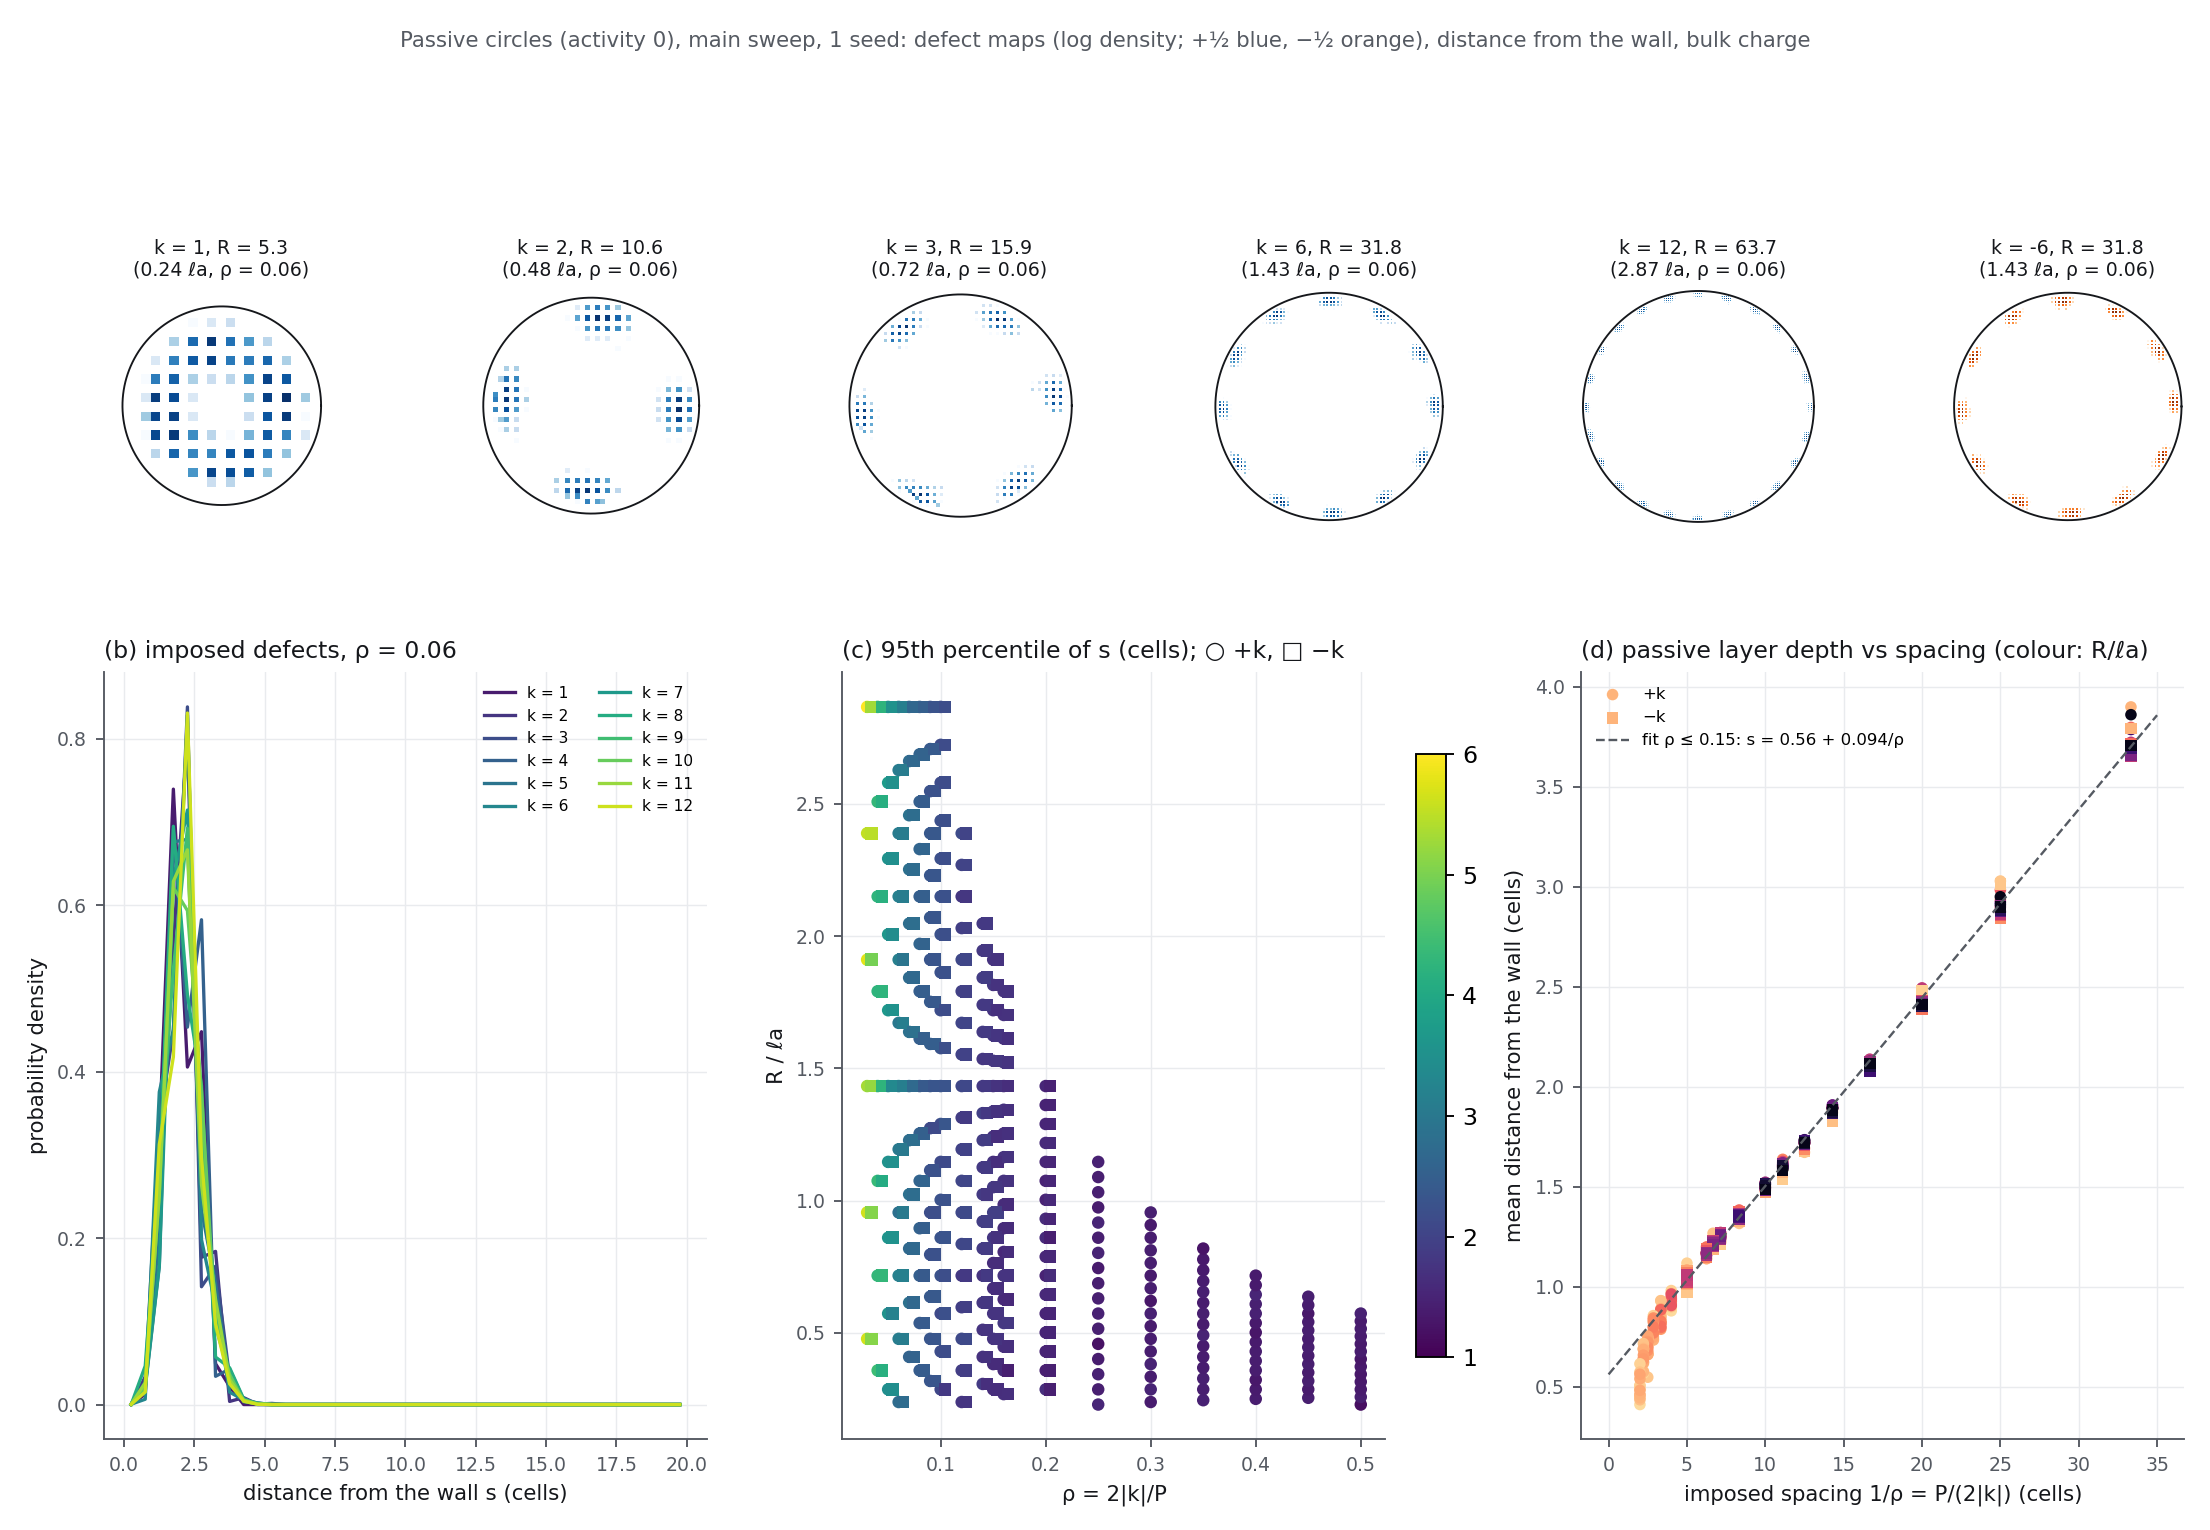
\includegraphics[width=\textwidth]{passive_circles.png}
\caption{Passive circles. (a) Time-averaged defect density (log scale, $+\half$ blue, $-\half$ orange) for $k=1,2,3,6,12$
at $\rho=0.06$ and for $k=-6$: the defects sit on $2|k|$ fixed sites just inside the wall. (b) Distribution of the distance
$s$ from the wall of the imposed defects, $k=1\dots12$ at $\rho=0.06$: the same narrow peak at $s\approx2$ cells for every
$k$. (c) 95th percentile of $s$ over the sweep ($\circ$ $+k$, $\square$ $-k$): it depends on $\rho$ only. (d) Mean $s$
against the imposed spacing $1/\rho$, all 468 runs (colour $R/\la$): a single line,
$\langle s\rangle\approx0.56+0.094/\rho$ cells for $\rho\le0.15$, identical for both signs.}\label{fig:passive}
\end{figure}

\paragraph{Results.}
\begin{itemize}
  \item \textbf{Every imposed defect is present, and nothing else.} $N_\pm$ per frame equals $2|k|$ of the imposed sign
        and 0 of the other sign to two decimals in every run with $\rho\le0.15$; the median fraction of frames with exactly
        this configuration is 0.994. At $\rho=0.20$ it drops to 0.76--0.90, the anchoring resolution limit
        (Sec.~\ref{sec:resolution}).
  \item \textbf{They sit on fixed sites} at equal spacing along the wall (Fig.~\ref{fig:passive}a), $2|k|$ of them;
        the time-averaged maps show compact spots, so the defects do not move along the wall (their apparent speed,
        0.3 cells per time unit, is the detection jitter of the cell-based tracker; Fig.~\ref{fig:prof-circ}).
  \item \textbf{Their depth is set by the imposed spacing only} (Fig.~\ref{fig:passive}d): the mean distance from the wall
        grows linearly with $1/\rho$, from $\approx1$ cell at $\rho=0.2$ (spacing 5) to 3.9 cells at $\rho=0.03$ (spacing 33),
        independent of $R$ and of the sign of $k$. A defect sits deeper when its neighbours along the wall are farther
        away, as expected for a director field that relaxes the imposed winding over a distance comparable with the spacing.
  \item This explains two observations that looked like exceptions earlier. In the $R=15$ validation run, $k=1$ placed its
        two $+\half$ at $r\approx9$--10, i.e.\ $s\approx5$--6: the spacing is 47 cells, where the line predicts 5.0. In the
        passive fixed-radius scan ($R=31.8$), $k=2$ sat at $s\approx5.7$ (spacing 50, predicted 5.3), which was read as
        ``no layer''; across that scan ($\rho=0.02$--0.10) the passive layer shrank from 8.3 to 2.3 cells with $k$ for the same
        reason. A passive ``layer width'' is therefore not a good edge for the active bulk (Sec.~\ref{sec:edge}).
  \item \textbf{Bulk charge 0.} The charge enclosed inside the defect ring is zero in every frame: all charge is in the
        wall layer. A fixed cut at 5 cells from the wall wrongly counts some wall defects as bulk at $\rho\le0.04$, where
        the layer is deeper than 5 cells (up to $|q|\approx0.95$ at $\rho=0.03$, $R=2.9\,\la$); this is a cut artefact, not
        a bulk charge.
  \item \textbf{Mirror symmetry is exact.} With $-k$ the same number of $-\half$ appears at the same depths
        (Fig.~\ref{fig:passive}d, squares); at $R=15$, $k=-2,-3$ reproduce $k=2,3$ (alignment 0.99, $Q(R-1)=-2.00/-3.00$).
        Any asymmetry between the signs in active runs is therefore an active effect.
  \item \textbf{Anchoring quality.} At $R=15$ the wall director follows the imposed winding with alignment 0.96--0.99;
        \texttt{customAnch} = 0 and 1 give identical results.
\end{itemize}

%=====================================================================
\section{Active circles: where the defects sit}\label{sec:cdist}
\subsection{Maps and profiles across sizes}
Figure~\ref{fig:maps-circ} shows the time-averaged defect density of active circles with $k=6$ and five radii,
$R=0.57$, 0.86, 1.43, 2.15 and $2.87\,\la$ (main sweep, seed 1, $\zeta=0.07$), together with one passive circle of $k=6$ at
$R=1.43\,\la$. Because $k$ is fixed, the imposed density $\rho=k/(\pi R)$ falls as the cavity grows (0.15, 0.10, 0.06, 0.04,
0.03), so this series changes size and density together; the dependence on $k$ at fixed size is in Sec.~\ref{sec:cdist-k}, and the full
$(\rho,R/\la)$ plane in Sec.~\ref{sec:sweep}. Figure~\ref{fig:prof-circ} gives, for the same runs, the $+\half$ and $-\half$
densities and the $+\half$ speed against the distance from the wall in units of $\la$ (method: Sec.~\ref{sec:m-dist}).

\begin{figure}[H]\centering
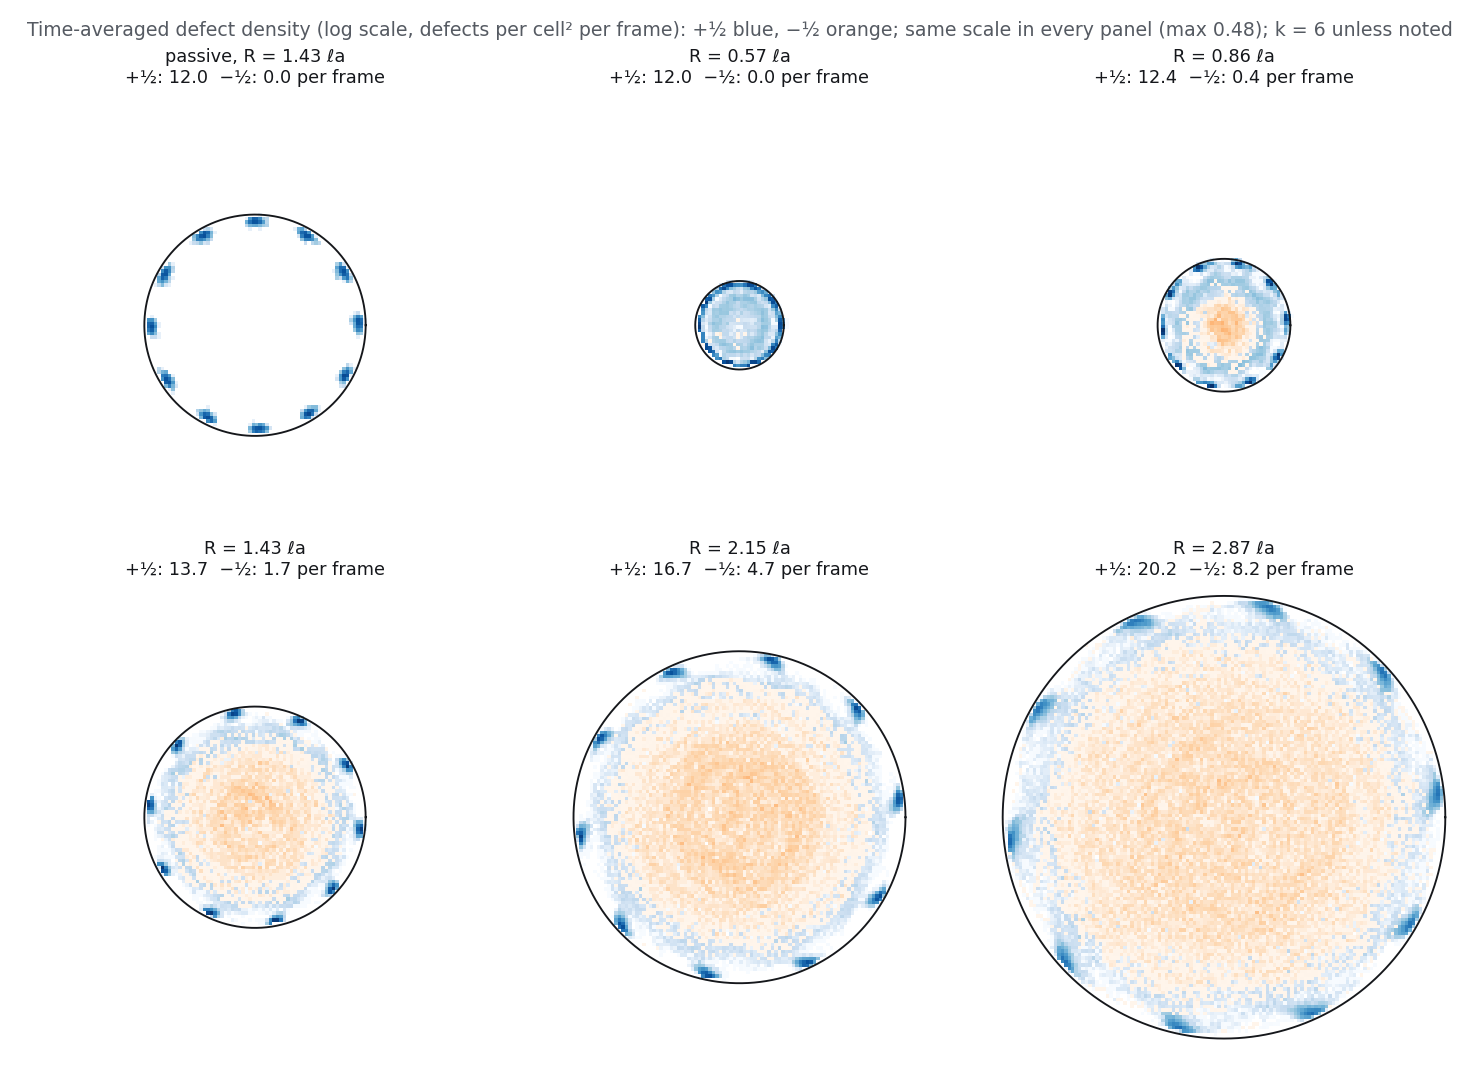
\includegraphics[width=0.92\textwidth]{maps_circles.png}
\caption{Time-averaged defect density, circles with $k=6$ (seed 1; log scale, the same scale in every panel; $+\half$ blue,
$-\half$ orange; per-frame counts in the panel titles, $N_+-N_-=2k=12$ in every run). Passive: 12 fixed spots at the wall.
$R=0.57\,\la$: no $-\half$, so no bulk; $\approx11$ of the 12 $+\half$ at the wall, already in a 10-site pattern but weakly
pinned, the 12th just inside. $0.86\,\la$: the first $\pm\half$ pairs (0.4 per frame); 10 $=2k-2$ wall sites. $1.43\,\la$: 10 pinned
sites, a ring of mobile $+\half$ just inside them, $-\half$ densest in the centre. $2.15$ and $2.87\,\la$: more pairs (4.7 and
8.2 per frame), $-\half$ spread over the whole inner half; the 10 sites persist, but at $2.87\,\la$ only $\approx7.6$ are occupied
at a time and the spots are elongated along the wall.}\label{fig:maps-circ}
\end{figure}

\begin{figure}[H]\centering
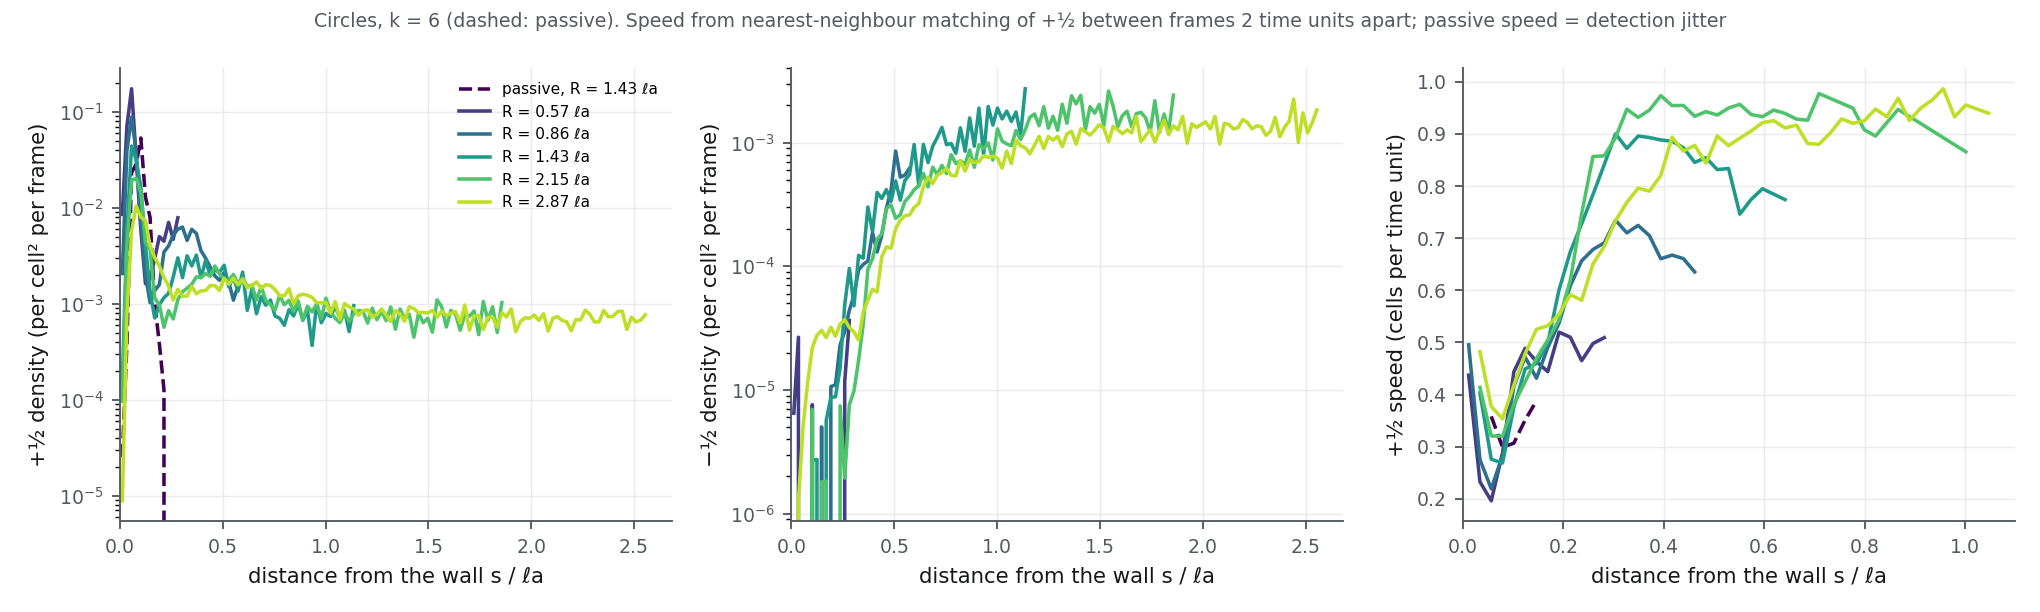
\includegraphics[width=\textwidth]{profiles_circles.png}
\caption{Circles, $k=6$: $+\half$ density, $-\half$ density and $+\half$ speed against the distance $s$ from the wall
(units of $\la$; dashed: passive). The $+\half$ density has a sharp wall peak at $s\approx1$--2 cells
($s/\la\approx0.05$--0.1), a depleted gap just inside it, and a flat bulk plateau ($\approx8\times10^{-4}$ per cell$^2$ per
frame, the same at every size). The $-\half$ are excluded from the outer $\approx0.3\,\la$ and uniform beyond $\approx0.7\,\la$.
Wall $+\half$ move at the passive jitter level (0.2--0.35 cells per time unit); the speed rises across the gap to
0.9--1.0 in the bulk of the larger cavities (lower in small cavities, where the bulk is close to the wall).}\label{fig:prof-circ}
\end{figure}

\begin{itemize}
  \item \textbf{Three zones.} A wall layer of pinned $+\half$ (peak at 1--2 cells), a gap at $s\approx3$--5 cells where both
        the density and the speed change, and a bulk of mobile $+\half$ and $-\half$ (structure below). The gap and the
        speed step sit at the same distance, which is what the density-minimum edge uses (Sec.~\ref{sec:edge}).
  \item \textbf{Size} (Fig.~\ref{fig:maps-circ}; numbers from the wall Fourier analysis, Sec.~\ref{sec:clattice}).
        At $0.57\,\la$ there are no bulk pairs: $\approx10.9$ $+\half$ are within the wall band, arranged with the 10-site
        ($2k-2$) period but only weakly pinned (static fraction 0.51, lattice memory 0.55); the remaining $+\half$ sits just
        inside. From $0.86\,\la$ pairs appear and the sites pin (static fraction 0.83 at 0.86, 0.99 at 1.43 and $2.15\,\la$).
        At $2.87\,\la$ the lattice still sits at fixed sites (lattice memory 0.97, static fraction 0.86) but is under-occupied,
        7.6 of 10 on average: the layer degrades by vacancies, not by sliding.
  \item \textbf{Bulk.} Up to $1.43\,\la$ the $-\half$ are densest in the centre ($3.5\times$ the density at $r/R=0.5$--0.75) and
        the bulk $+\half$ form a ring just inside the wall sites ($2.5\times$ the central density). In the larger cavities the
        $-\half$ fill the inner half uniformly; both signs are depleted only within $\approx0.3\,\la$ of the wall. Because the
        $-\half$ stay away from the wall, the accumulated charge $Q(r)$ dips below 0 inside before rising to the $+1$ plateau
        (Sec.~\ref{sec:ccharge}).
  \item The wall peak of the $+\half$ density falls with size (0.044 per cell$^2$ at $1.43\,\la$, 0.010 at $2.87\,\la$) mostly
        because the same $\approx10$ wall defects are spread along a longer wall; it is not by itself a sign of a weaker layer.
\end{itemize}

\subsection{Dependence on $k$ at fixed size}\label{sec:cdist-k}
\begin{figure}[H]\centering
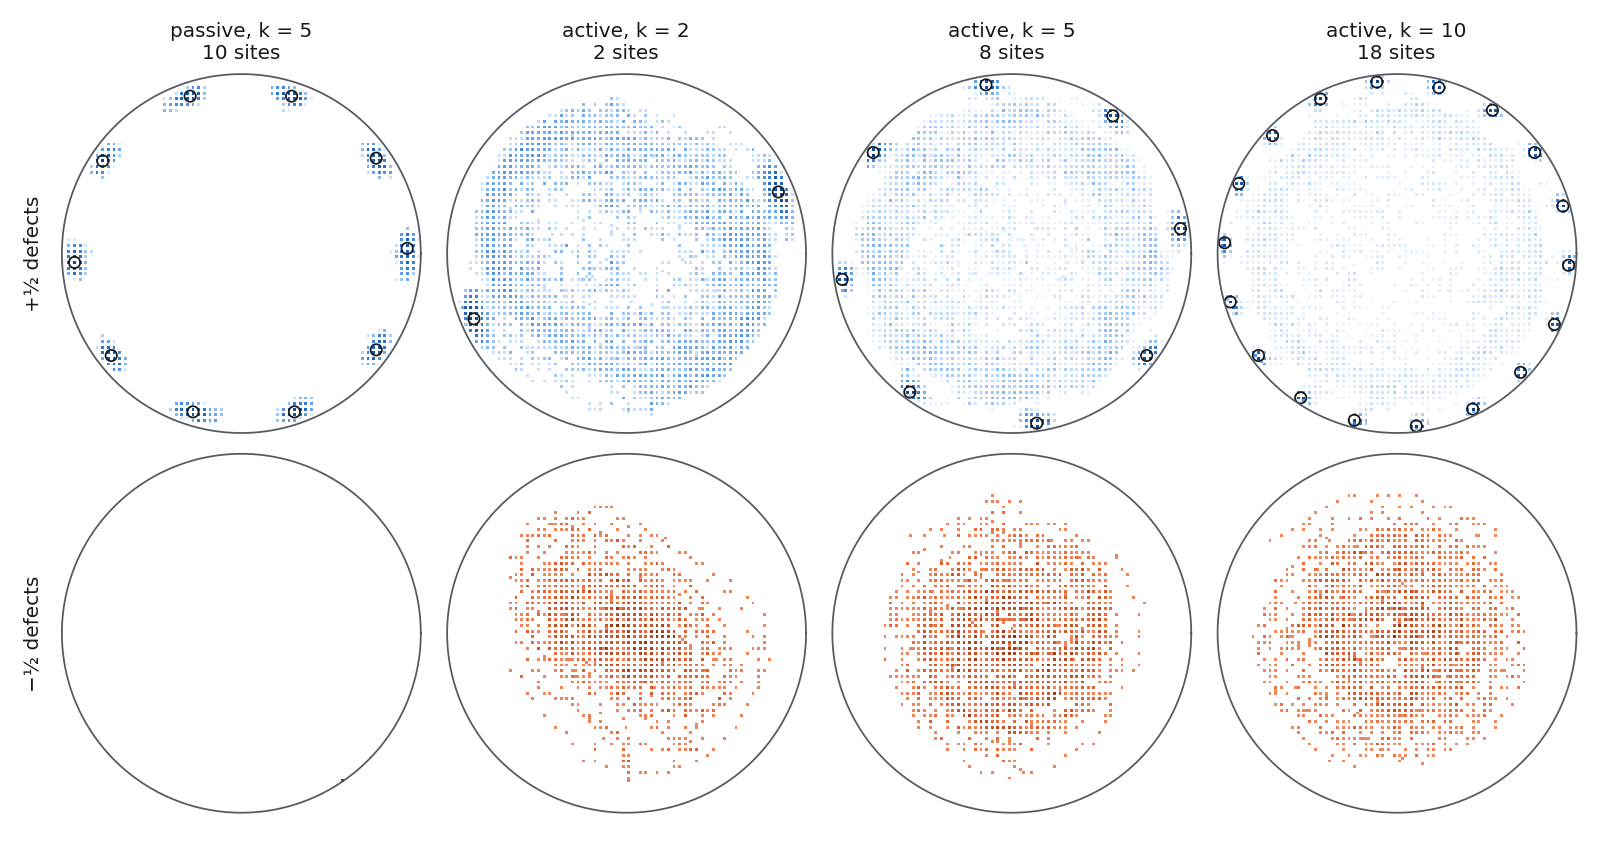
\includegraphics[width=\textwidth]{circle_maps_k.png}
\caption{Time-averaged density of $+\half$ (top) and $-\half$ (bottom), $R=1.43\,\la$: passive $k=5$ and active $k=2,5,10$
(seed 2). Open circles: pinned sites from the site rule, $2k$ passive and $2k-2$ active.}\label{fig:maps-k}
\end{figure}
\begin{figure}[H]\centering
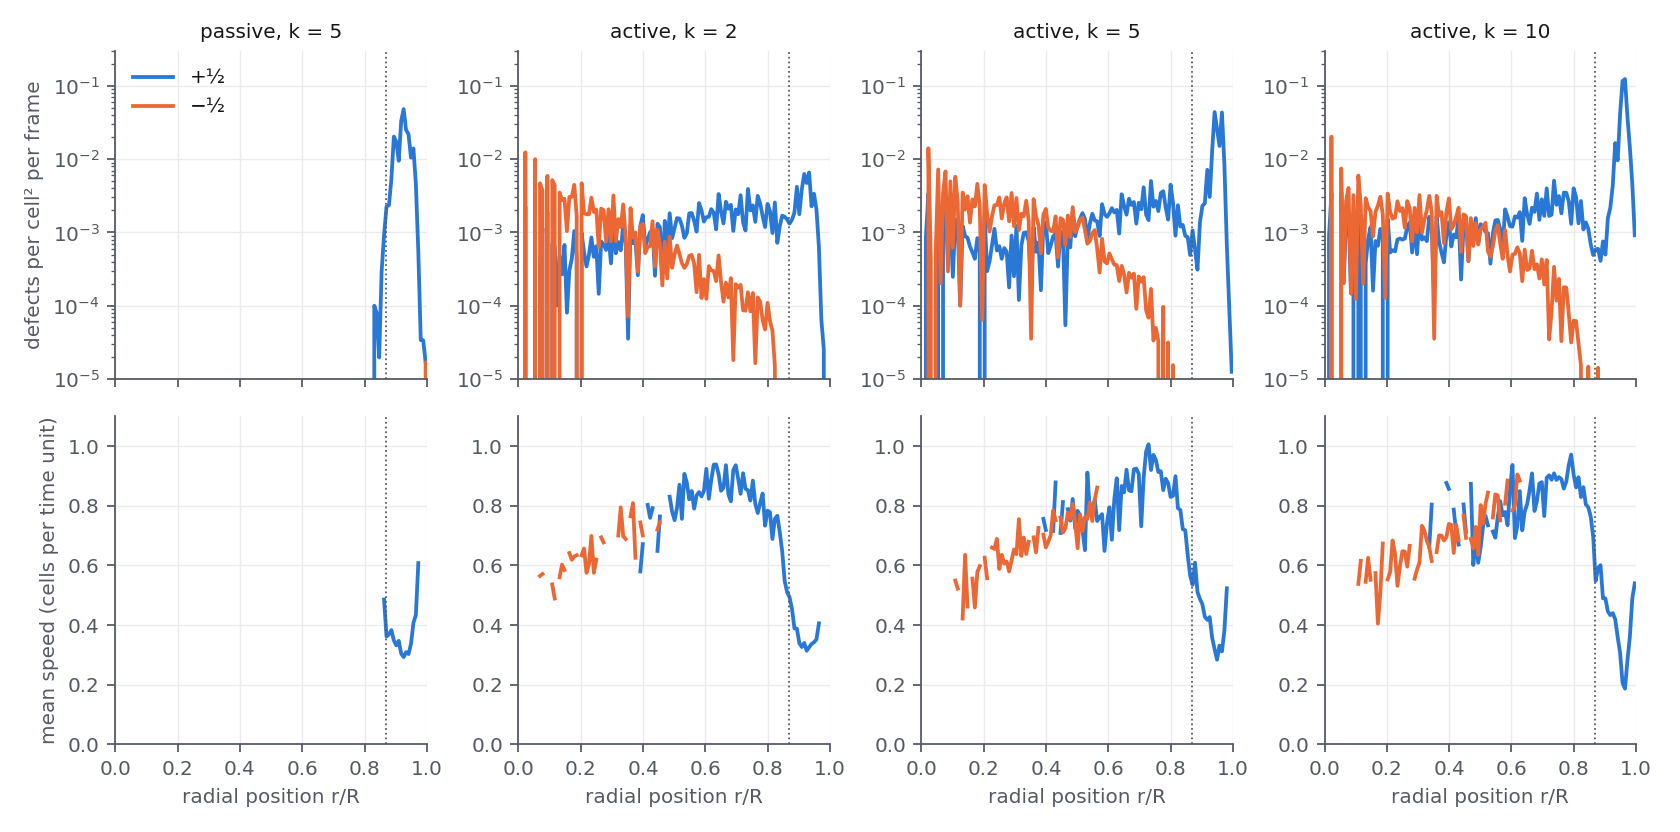
\includegraphics[width=\textwidth]{circle_radial.png}
\caption{Radial profiles at $R=1.43\,\la$ for the runs of Fig.~\ref{fig:maps-k}: $+\half$ and $-\half$ density and speed
against the distance from the wall.}\label{fig:radial-k}
\end{figure}
\begin{itemize}
  \item The number of wall sites is $2k-2$ in every active run of the fixed-radius scan (27/27 runs, $k=2\dots10$, 3 seeds),
        against $2k$ in the passive runs: two $+\half$ have left the wall to form the $+1$ bulk.
  \item The layer is diffuse and thicker at low $k$ and sharp at high $k$ (the spacing argument of Sec.~\ref{sec:passive}
        applies to the active layer too); the bulk is the same at every $k$.
  \item The capture distance of the site rule (minimum of the distance-to-nearest-site histogram, Fig.~\ref{fig:sitedist})
        shrinks with $k$ from 6.2 to 3.1 cells, about half the site spacing.
\end{itemize}
\begin{figure}[H]\centering
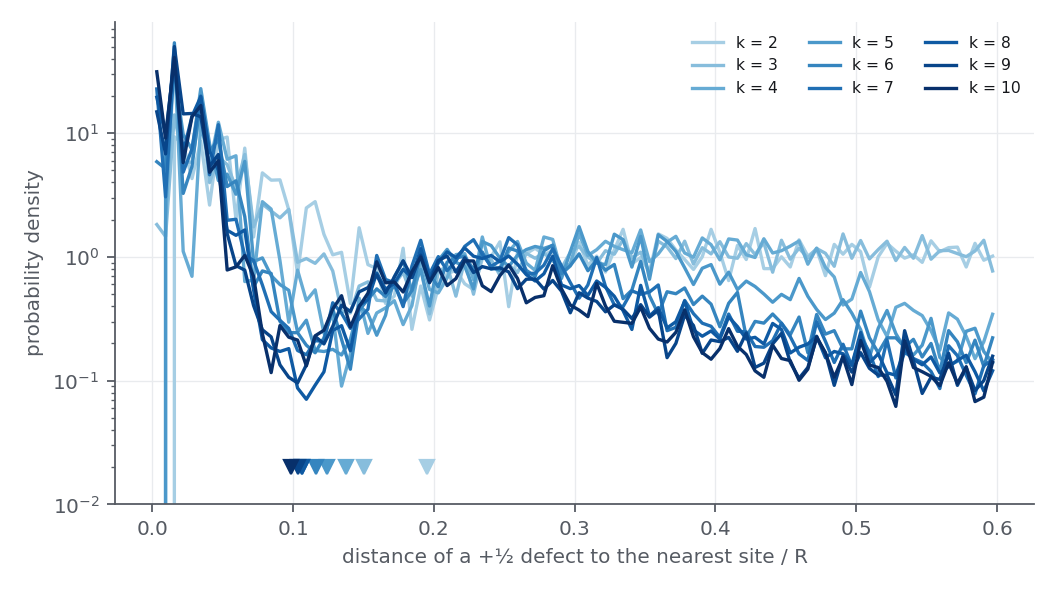
\includegraphics[width=0.85\textwidth]{circle_sitedist.png}
\caption{Distance of each $+\half$ to the nearest pinned site (histograms per run). The minimum separates defects on a
site (edge) from the rest (bulk) and defines the capture distance of the site rule.}\label{fig:sitedist}
\end{figure}

\subsection{Pair correlations}\label{sec:gr}
\SIcand
Ring-resolved pair correlations $g_{ab}(r\,|\,s)$ (reference defect binned by its distance $s$ from the wall, partner
anywhere, the radial profile divided out; method in Sec.~\ref{sec:m-gr}), pooled over $k$ and seeds of the fixed-radius scan.
\begin{figure}[H]\centering
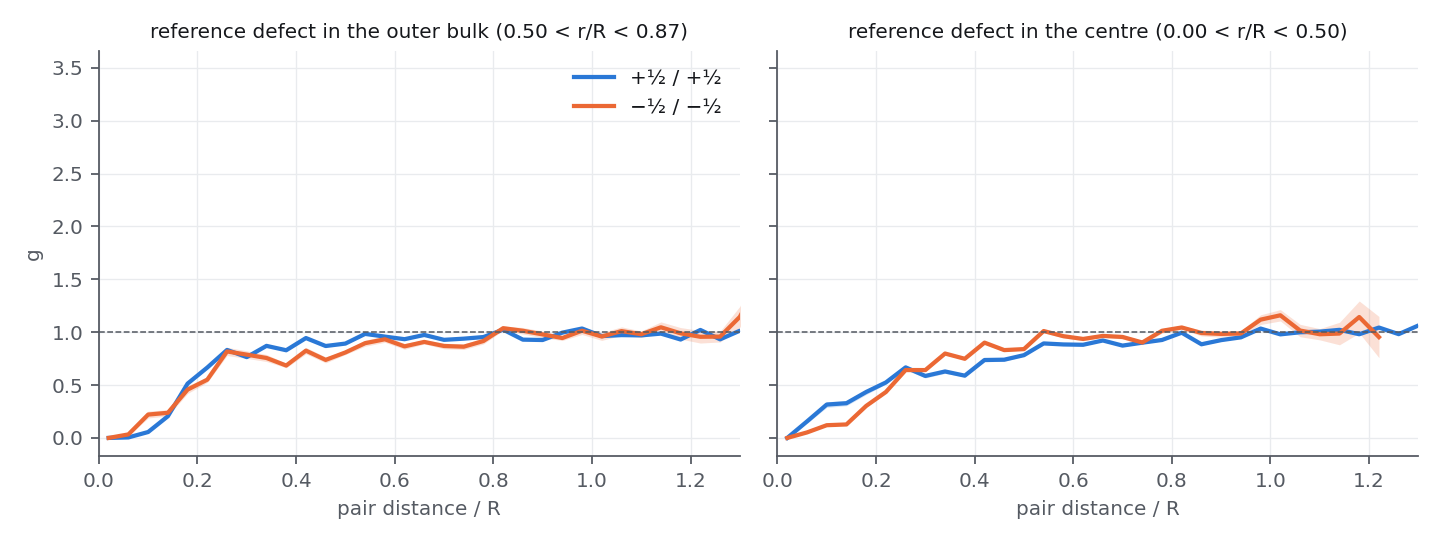
\includegraphics[width=0.49\textwidth]{g_same.png}\hfill
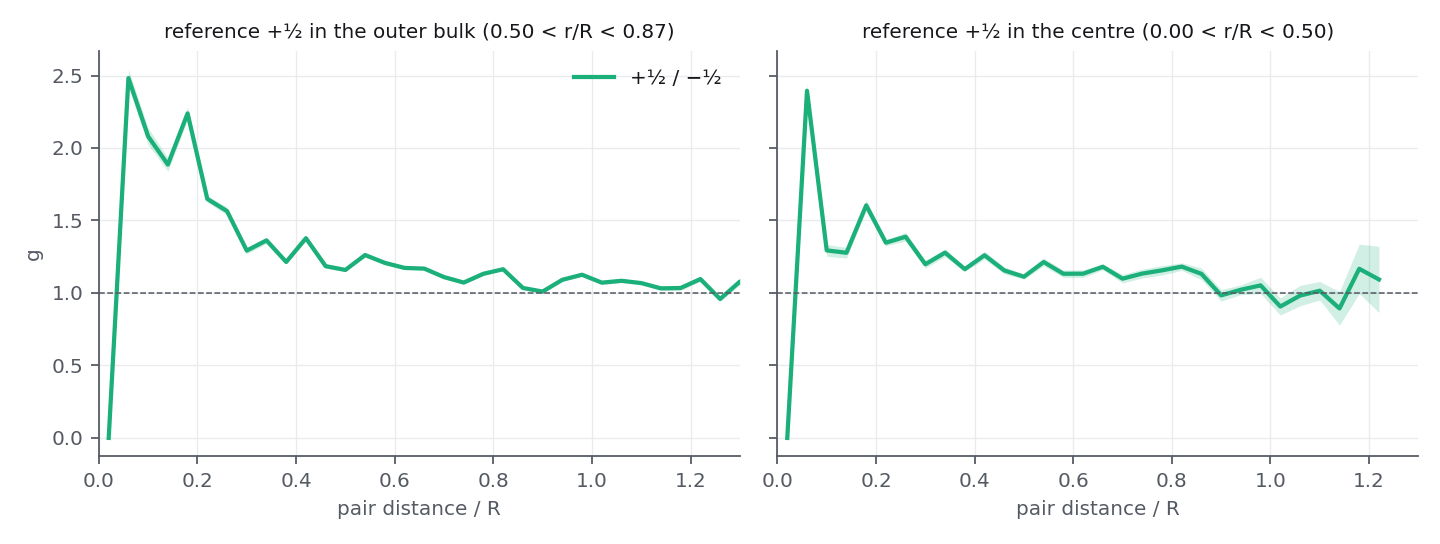
\includegraphics[width=0.49\textwidth]{g_pm.png}
\caption{Left: like-sign correlations $g_{++}$ (blue) and $g_{--}$ (orange) against the pair distance in units of $R$,
with the reference defect in the outer bulk ($0.5<r/R<0.87$) and in the centre ($r/R<0.5$); both have the same hole,
recovering to 1 at $\approx0.5$--$0.6R\approx\la$. Right: $g_{+-}$ for the same zones. $R=1.43\,\la$, pooled over
$k=2\dots10$ and 3 seeds; bands: Poisson error.}\label{fig:g}
\end{figure}
\begin{figure}[H]\centering
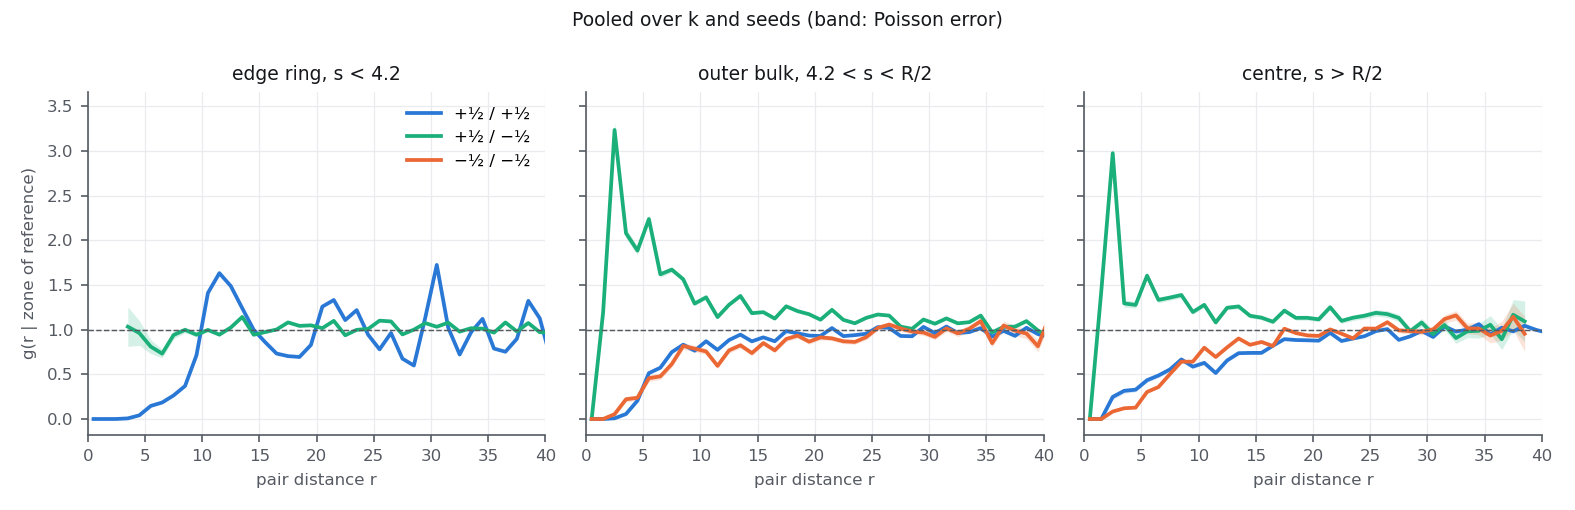
\includegraphics[width=0.9\textwidth]{g_zones.png}
\caption{Pooled $g(r\,|\,\text{zone})$ in cells, reference defect in the edge ring ($s<4.2$), the outer bulk
($4.2<s<R/2$) or the centre ($s>R/2$). Edge ring: $+\half/+\half$ lattice peaks at the site spacing ($\approx11$ cells
pooled over $k$) and its multiples; $+\half/-\half\approx1$. Bulk zones: $+\half/-\half$ peak $g\approx3$ at 2.5 cells;
like signs depleted below $\approx15$ cells.}\label{fig:gzones}
\end{figure}
\begin{itemize}
  \item \textbf{Bulk:} $+\half/-\half$ peak at $g\approx3.2$ at $r\approx2.5$ cells (fresh or annihilating pairs), with a tail
        above 1 out to 20--25 cells. Like signs have the same correlation hole: $g\approx0$ for $r<3$, 0.5 at $r\approx6$,
        1 at $r\approx15$--20 cells, i.e.\ about $\la$. The hole is slightly longer in the centre.
  \item \textbf{Wall ring:} $+\half/+\half$ lattice peak at the site spacing; $+\half/-\half\approx1$, so layer defects do
        not bind $-\half$.
  \item In units of $r/R$ ($\propto r/\la$ at fixed $R/\la$) the bulk $g_{++}$ collapses for $\zeta=0.05$, 0.07 and 0.09;
        $g_{--}$ collapses only up to $\approx0.5R$ at $\zeta=0.05$ (Sec.~\ref{sec:activity}).
  \item Known artefact: a red diagonal at the largest $r$ in the per-$k$ maps (partner in the far-side layer) comes from the
        thin layer peak in the expectation, not from a correlation.
\end{itemize}

%=====================================================================
\section{Active circles: the $+1$ bulk and the wall layer}\label{sec:ccharge}
\subsection{Fixed size, all windings: $R=1.43\,\la$, $k=2\dots10$}
The cleanest test: $R=31.83$ ($R/\la=1.43$), $k=2\dots10$ ($\rho=0.02$--0.10, $\rho\la=0.44$--2.2), 3 seeds, 10k warm-up + 40k
steps. Two independent edge rules (Sec.~\ref{sec:edge}): the density minimum $d_\rho$ and the pinned-site rule.
\begin{table}[H]\centering\small
\caption{Fixed-radius scan, mean $\pm$ s.e.\ over 3 seeds. $q_b$: bulk charge per frame; $P_1$: fraction of frames with
$q_b=+1$ exactly; $d_\rho$: density-minimum edge (cells from the wall); $N_L$: $+\half$ in the layer; sites: pinned sites
found; agree: fraction of $+\half$ classified identically by the two rules. Last two columns: the passive layer width
used as the edge instead, which fails (Sec.~\ref{sec:passive}).}\label{tab:rscan}
\begin{adjustbox}{max width=\textwidth}
\begin{tabular}{rcccccccc|cc}\toprule
$k$ & $q_b$ (density) & $P_1$ & $d_\rho$ & $N_L$ & sites & $q_b$ (sites) & $P_1$ (sites) & agree & $q_b$ (passive edge) & $P_1$\\\midrule
2 & $1.03\pm0.02$ & 0.83 & 4.6 & 1.9 & 2 & $1.01\pm0.01$ & 0.91 & 0.956 & $0.44\pm0.05$ & 0.26\\
3 & $1.01\pm0.01$ & 0.90 & 4.2 & 4.0 & 4 & $1.03\pm0.01$ & 0.89 & 0.981 & $0.83\pm0.01$ & 0.69\\
4 & $0.99\pm0.00$ & 0.92 & 4.2 & 6.0 & 6 & $1.01\pm0.00$ & 0.94 & 0.990 & $0.98\pm0.01$ & 0.92\\
5 & $0.99\pm0.01$ & 0.90 & 4.2 & 8.0 & 8 & $1.02\pm0.01$ & 0.93 & 0.992 & $1.04\pm0.02$ & 0.90\\
6 & $1.01\pm0.01$ & 0.90 & 4.1 & 10.0 & 10 & $1.02\pm0.01$ & 0.94 & 0.993 & $1.07\pm0.01$ & 0.85\\
7 & $1.01\pm0.02$ & 0.89 & 4.2 & 12.0 & 12 & $1.05\pm0.02$ & 0.91 & 0.994 & $1.15\pm0.03$ & 0.74\\
8 & $1.00\pm0.00$ & 0.95 & 3.8 & 14.0 & 14 & $1.01\pm0.00$ & 0.96 & 0.997 & $1.18\pm0.01$ & 0.68\\
9 & $1.01\pm0.01$ & 0.94 & 3.8 & 16.0 & 16 & $1.02\pm0.02$ & 0.95 & 0.997 & $1.17\pm0.03$ & 0.71\\
10 & $1.04\pm0.03$ & 0.89 & 3.8 & 17.9 & 18 & $1.09\pm0.06$ & 0.90 & 0.994 & $1.20\pm0.04$ & 0.71\\\bottomrule
\end{tabular}
\end{adjustbox}
\end{table}
\begin{itemize}
  \item \textbf{The bulk carries $+1$ at every $k$}, to within 0.04, and is exactly $+1$ in 83--96\% of frames. The layer holds
        $N_L=2k-2$ of the $+\half$ (charge $k-1$) on exactly $2k-2$ pinned sites. The two rules agree on 96--99.7\% of all
        $+\half$; the lowest agreement is at $k=2$, where the layer is diffuse.
  \item The fluctuations are dynamical $\pm\half$ pairs (1.5--2.0 per frame) and occasional transients (one seed at $k=10$).
        Every run has a strong steady vortex (circulation order parameter $\Phi=0.89$--0.97).
  \item \textbf{The effect does not fade at low density} (H2 not supported): $q_b=+1$ down to $\rho=0.02$ ($\rho\la=0.44$),
        far below the predicted crossover $\rho\la\approx1$.
  \item A fixed cut 2.5 cells from the wall splits the layer and reports 1.2--1.5; the passive layer width is the wrong edge
        too (last columns). The bulk/layer boundary has to come from the active data themselves.
\end{itemize}
\begin{figure}[H]\centering
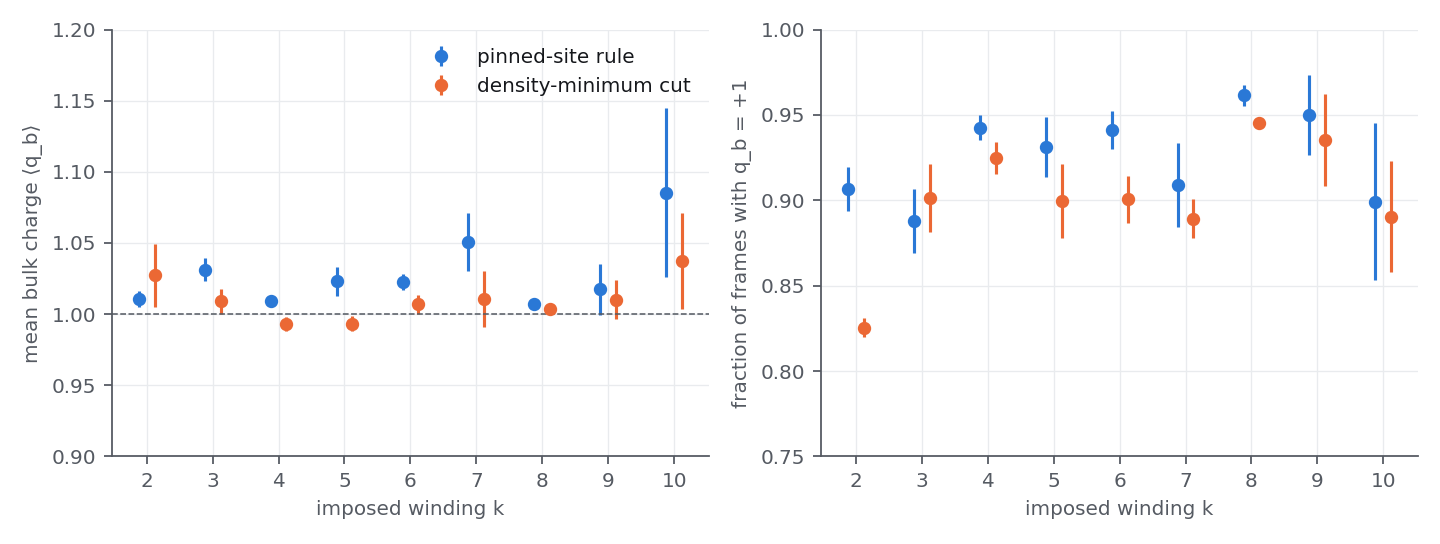
\includegraphics[width=0.85\textwidth]{circle_bulkcharge_rules.png}
\caption{Fixed-radius scan ($R=1.43\,\la$, 3 seeds): mean bulk charge (left) and fraction of frames with $q_b=+1$ (right) against $k$, pinned-site rule (blue) and density-minimum cut (orange).}\label{fig:rules}
\end{figure}

\subsection{Cut-free criteria: mobility and tilt}
Wall defects are slow and tilted; bulk defects are fast and point elsewhere (methods: Sec.~\ref{sec:edge}).
\begin{figure}[H]\centering
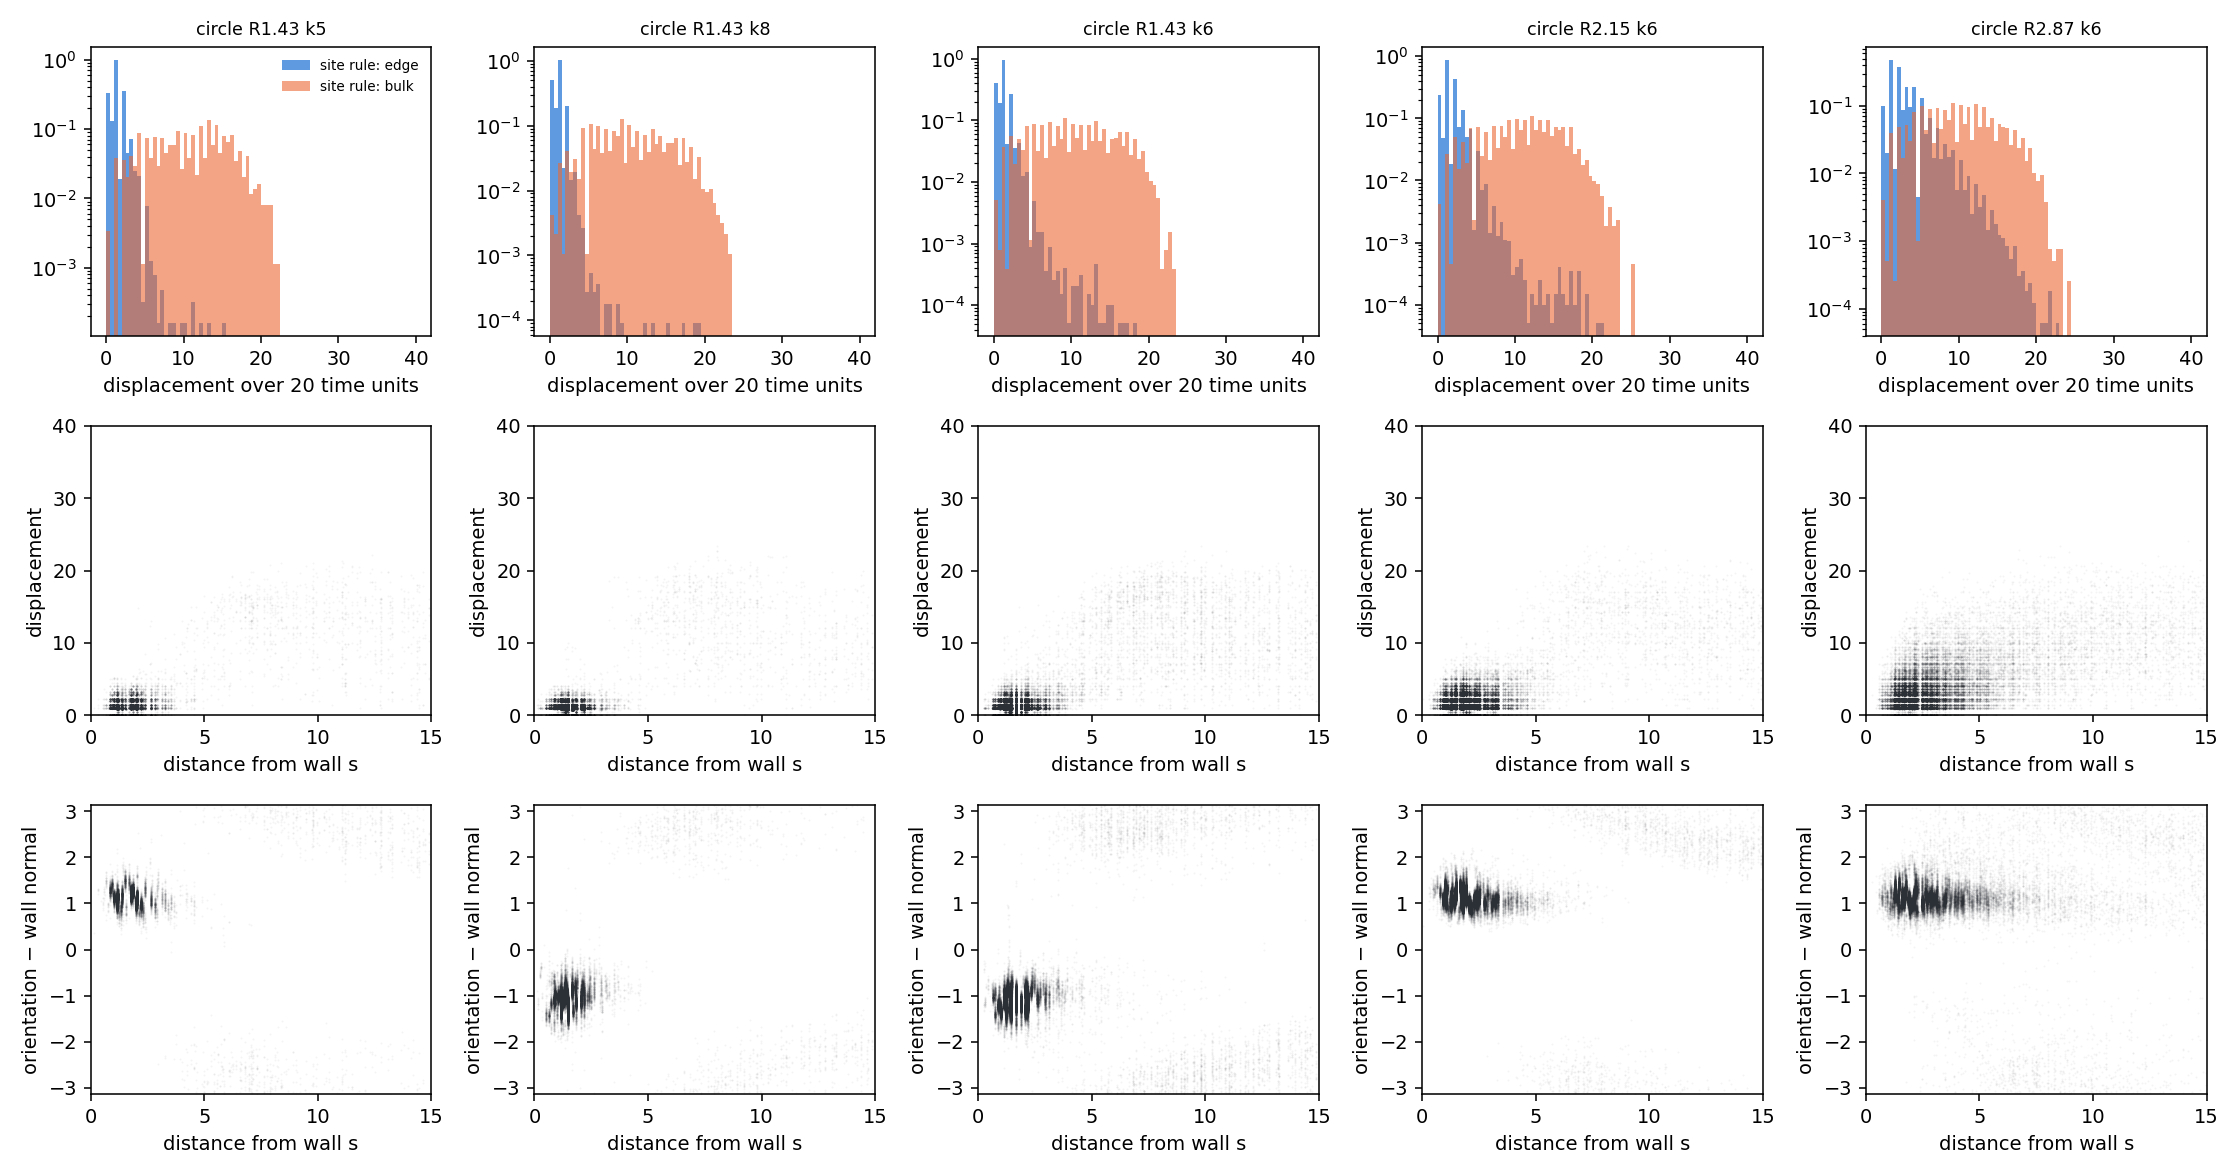
\includegraphics[width=\textwidth]{edge_criteria_circles.png}
\caption{Cut-free criteria on circles ($k=6$). Top: displacement over 20 time units, split by the site rule. Middle and
bottom: displacement and orientation relative to the outward wall normal against the distance from the wall.}\label{fig:crit}
\end{figure}
\begin{itemize}
  \item Wall defects: median displacement over 20 time units 1.0--1.4 cells against 10--11 in the bulk.
  \item \textbf{Tilt:} wall $+\half$ point at $|\Delta|\approx1.1$ rad ($\approx63^\circ$) from the outward normal, with the sign of
        the vortex sense in 6/6 runs; bulk $+\half$ cluster near $|\Delta|\approx\pi-0.5$. Nearly independent of $k$.
  \item Each criterion alone agrees with the site rule on 97--99\% of $+\half$ up to $2.15\,\la$ (89\% at $2.87\,\la$). With
        mobility, tilt or both, $q_b$ ($k=6$) is 1.05--1.07 at $1.43\,\la$, 1.11--1.25 at $2.15\,\la$ and 1.9--2.7 at $2.87\,\la$
        (site rule 1.85; part of the layer is tilted but mobile there).
\end{itemize}

\subsection{The whole parameter plane: main sweep}\label{sec:sweep}
834 active runs ($k=1$--20, $\rho=0.03$--0.50, 3 seeds; 10k + 100k steps) and 278 passive references. Every run was analysed
with the knee of $Q(r)$ (Sec.~\ref{sec:methods-knee}), $d^*$, $f^*$, the site rule and the wall Fourier analysis.
\begin{figure}[H]\centering
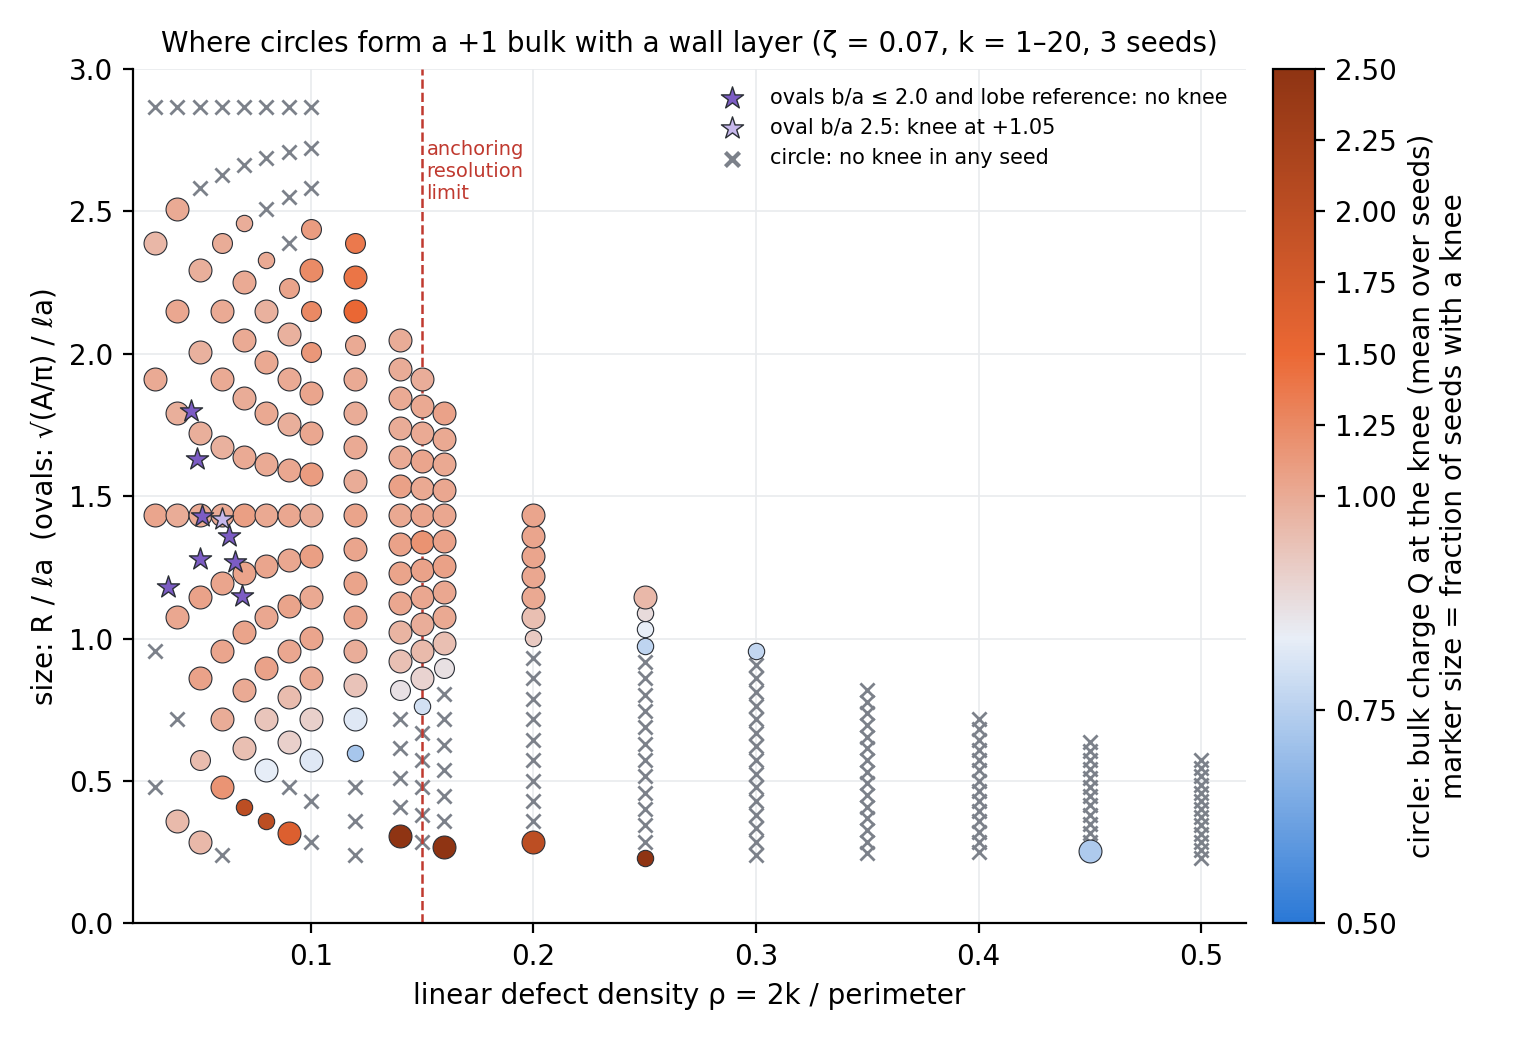
\includegraphics[width=0.85\textwidth]{layer_diagram_circles.png}
\caption{\textbf{Where circles have a $+1$ bulk and a wall layer.} Bulk charge at the knee of $Q(r)$ (colour; marker size =
fraction of seeds with a knee; crosses: no knee) over the linear defect density $\rho$ and the size $R/\la$. Stars: the
ovals at their own $\rho$ and equivalent radius $\sqrt{A/\pi}/\la$ (Part III).}\label{fig:diagram}
\end{figure}
\begin{table}[H]\centering\small
\caption{Main sweep, $\rho\le0.15$, all $k$, by size: fraction of runs with a knee, mean $Q$ at the knee, mean static
fraction of the wall lattice (1 = pinned; Sec.~\ref{sec:clattice}) and mean layer depth.}\label{tab:sweep}
\begin{adjustbox}{max width=\textwidth}
\begin{tabular}{lccccc}\toprule
$R/\la$ & runs & knee & $Q_\mathrm{knee}$ & $f_\mathrm{static}$ & $d^*/\la$\\\midrule
0.00--0.50 & 57 & 0.70 & 1.86 & 0.39 & 0.08\\
0.50--0.75 & 48 & 0.60 & 1.00 & 0.69 & 0.11\\
0.75--1.00 & 45 & 0.89 & 1.11 & 0.78 & 0.14\\
1.00--1.25 & 51 & 1.00 & 1.04 & 0.84 & 0.18\\
1.25--1.50 & 51 & 1.00 & 1.05 & 0.93 & 0.19\\
1.50--2.00 & 90 & 1.00 & 1.02 & 0.97 & 0.19\\
2.00--2.50 & 69 & 0.90 & 1.16 & 0.93 & 0.28\\
2.50--3.00 & 54 & 0.15 & 1.17 & 0.79 & 0.55\\\bottomrule
\end{tabular}
\end{adjustbox}
\end{table}
\begin{itemize}
  \item \textbf{Layer region: $R\approx0.75$ to $2$--$2.3\,\la$, at every density up to the resolution limit} (knee in 89--100\%
        of runs, $Q_\mathrm{knee}\approx1.0$, $f_\mathrm{static}\ge0.78$, $d^*\approx0.2\,\la\approx4.5$--6 cells).
  \item \textbf{Large cavities} ($\gtrsim2.5\,\la$): knee in 15\% of runs; the layer thickens ($d^*/\la=0.55$) and loses part
        of its sites. Degradation starts earlier at high $\rho$ (2.0--2.5\,$\la$: 42--48\% knees at $\rho\approx0.09$--0.13,
        100\% at low $\rho$).
  \item \textbf{Small cavities} ($\lesssim0.5$--$0.6\,\la$): no room for a bulk. The knee value tends to $k$ or is absent
        (e.g.\ $k=2$ at 0.36--0.48\,$\la$: knee at 1.6--2.0, i.e.\ no bulk pair at all).
  \item \textbf{Smallest clean circles} (the inscribed-radius test for the ovals, $\rho\approx0.06$): $k=3$, $R=0.72\,\la$:
        $Q_\mathrm{knee}=1.03$, $f_\mathrm{static}=0.97$, $d^*=0.16\,\la$; $k=4$, $0.96\,\la$: 1.07, 0.98, 0.17.
  \item Beyond the resolution limit ($\rho\ge0.2$) mostly no knee.
  \item \textbf{Knee finder:} with 5 smoothing bins it caught the flat shoulders of the cell-quantised layer steps (e.g.\
        $k=5$ at 0.80--0.90\,$\la$ gave a spurious knee at $Q\approx1.9$); 9 bins (0.045 in $r/R$) fixes it without moving genuine knees (Fig.~\ref{fig:knee}).
\end{itemize}
\begin{figure}[H]\centering
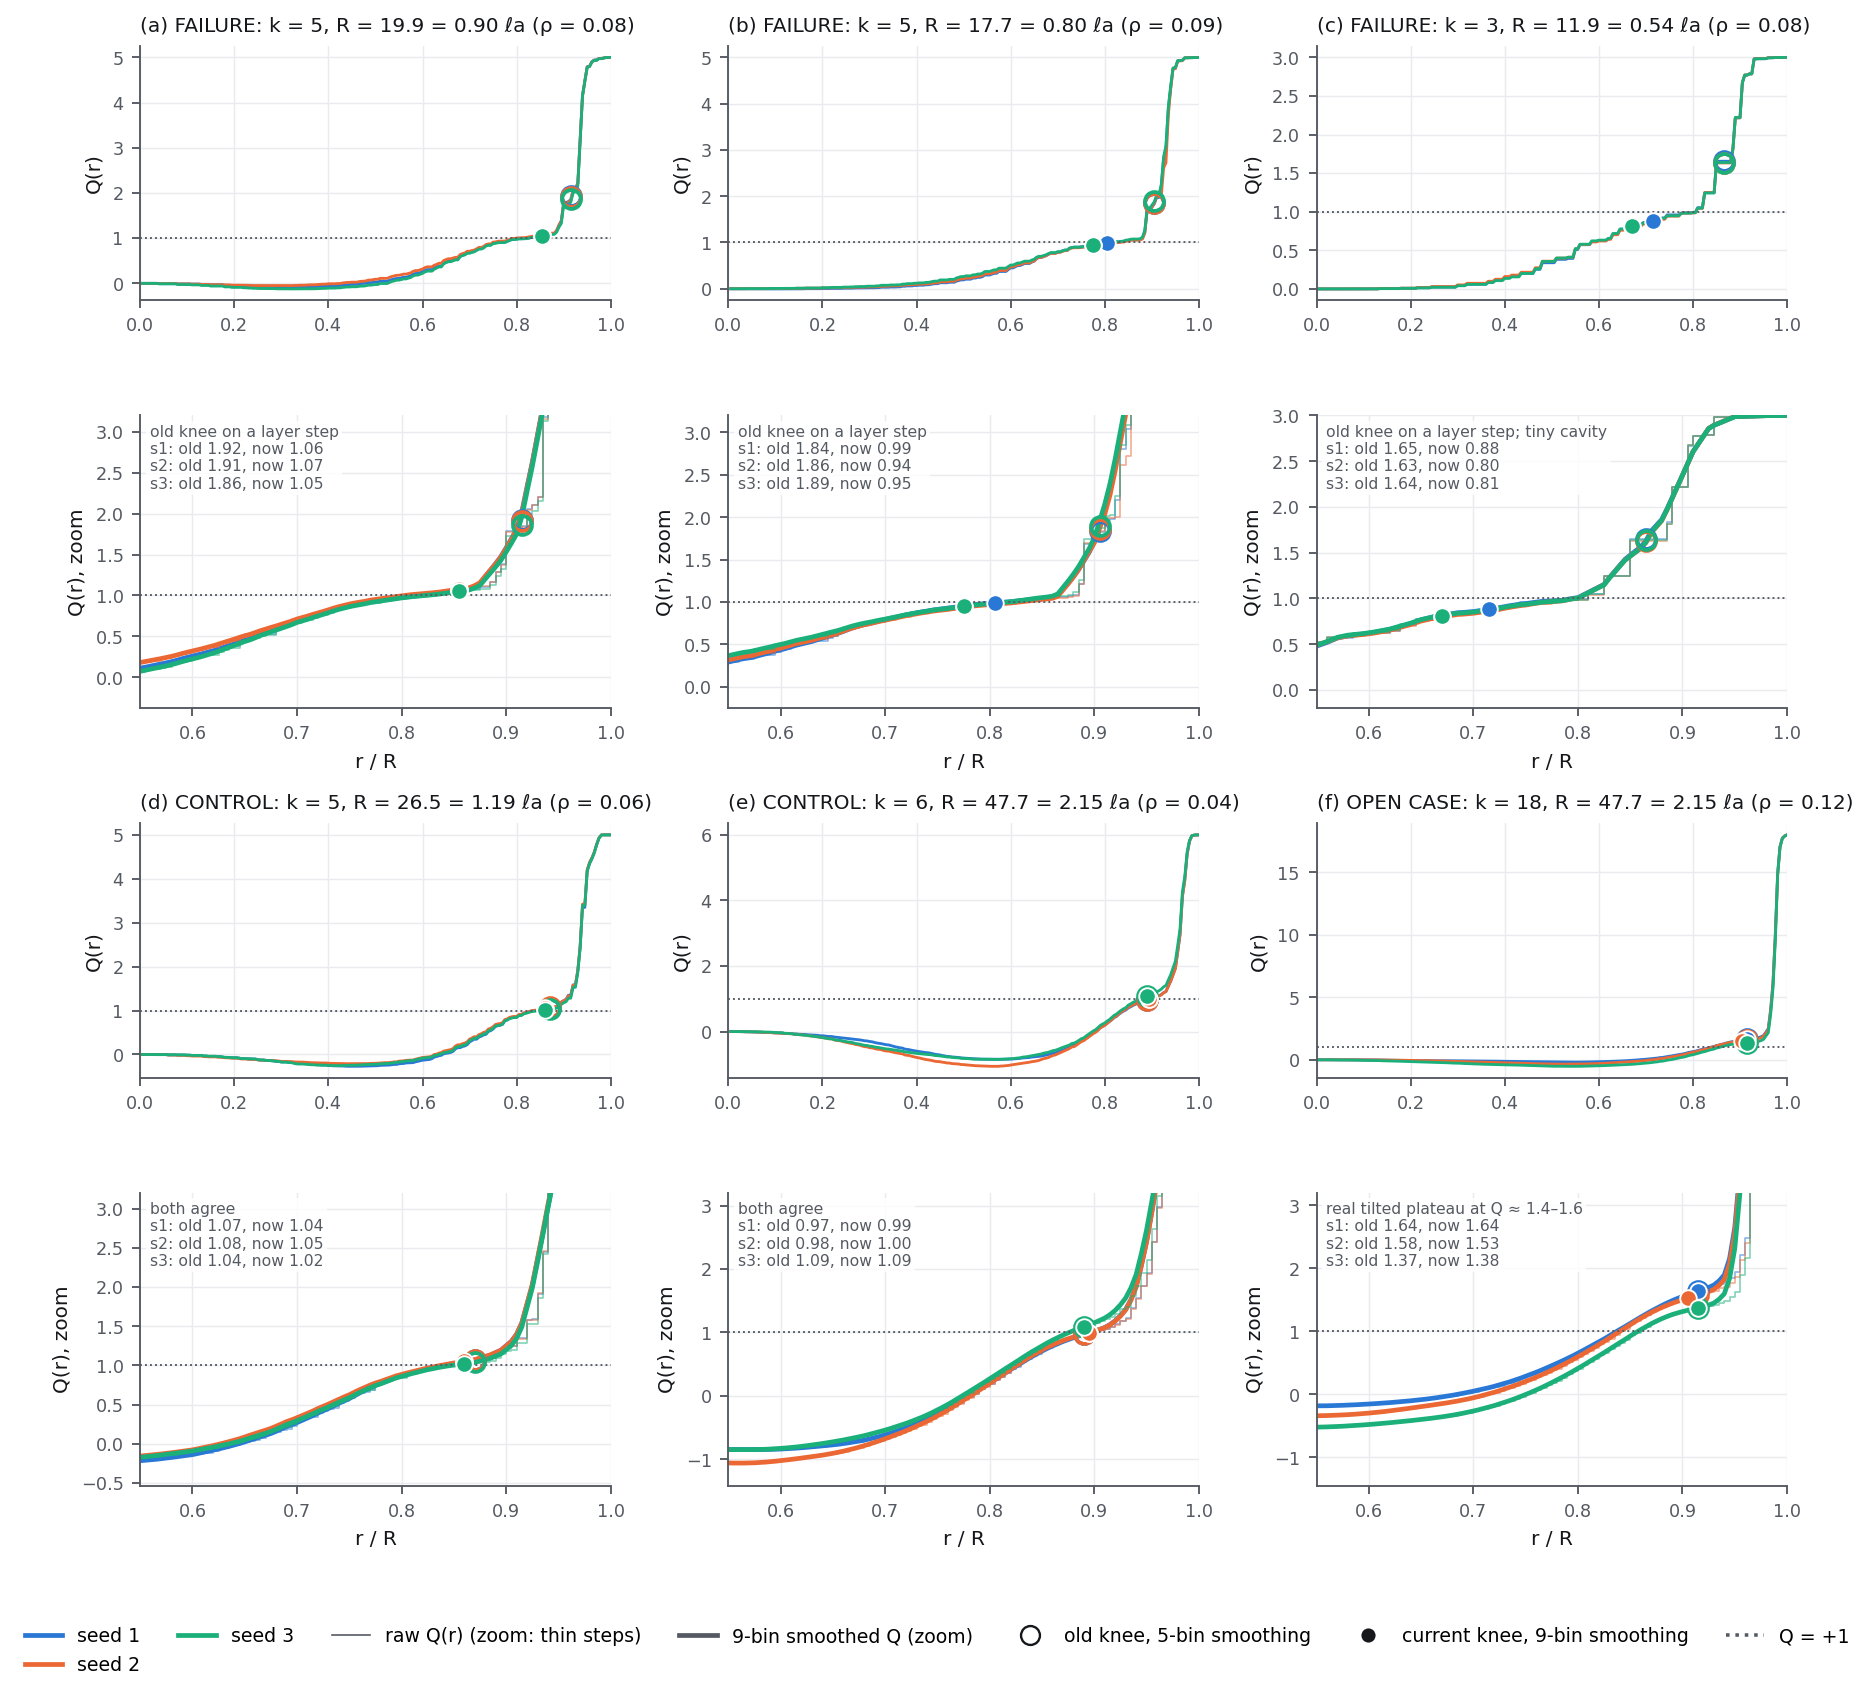
\includegraphics[width=\textwidth]{knee_check_v2.png}
\caption{\textbf{Why the knee finder smooths over 9 bins.} Six circles from the main sweep, three seeds each (blue, orange, green;
the seeds mostly overlap). For each run the upper panel shows the whole accumulated charge $Q(r)$ and the lower panel zooms on the
outer region, with the raw $Q(r)$ (thin steps) and the 9-bin smoothed $Q$ (thick). Open circles: knee found with the old 5-bin
smoothing; filled circles: knee with the current 9-bin smoothing (0.045 in $r/R$). The values per seed are printed in each zoom.
Close to the wall $Q$ climbs from $+1$ to $k$ in small steps, one per wall defect, each about 0.02 wide in $r/R$ because positions
are known to one cell.
(a, b) \emph{Failures of the old setting} ($k=5$, $R=0.90$ and $0.80\,\la$): with 5 bins a flat step part-way up the jump passes as a
plateau, and the finder reports a bulk charge of 1.84--1.92; 9 bins average the steps away and the knee moves inwards to the real
plateau, $Q=0.94$--1.07.
(c) \emph{Failure, and a limit of the method} ($k=3$, $R=0.54\,\la$): the old knee sits on a step at $Q\approx1.64$; the current knee
(0.80--0.88, at $r/R\approx0.7$) is better but still not the flattest part of $Q$, which is at $\approx1.0$ around $r/R\approx0.78$.
Cavities this small have hardly any bulk; their knee values are listed in Table~\ref{tab:sweep} for completeness but not read as a bulk charge.
(d, e) \emph{Controls} with a clear plateau ($k=5$ at $1.19\,\la$; $k=6$ at $2.15\,\la$): both settings give the same knee,
$Q=0.97$--1.09, so the wider smoothing does not shift genuine knees.
(f) \emph{Open case} ($k=18$, $R=2.15\,\la$, $\rho=0.12$): both settings find a shoulder at $Q\approx1.4$--1.6 just before the jump.
It is a real feature of $Q(r)$, not a step artefact: a candidate ``less-charged layer'' (see the box below).}\label{fig:knee}
\end{figure}
\open{A possible genuine ``less-charged layer'': large circles at high $\rho$ ($k=15$--20, $\rho=0.10$--0.12,
$R=2.0$--$2.6\,\la$) show a tilted plateau at $Q\approx1.3$--2.1 with all $2k-2$ sites pinned ($f_\mathrm{static}=0.65$--0.95).
Near both the resolution limit and the large-$R$ degradation; to be checked with 10 seeds.}

\subsection{Onset of the layer and the phase diagram}\label{sec:onset}
The knee of $Q(r)$ cannot show a bulk charge of 0: it needs a plateau, and a cavity too small to hold a bulk has none, so the knee is
undefined or picks up a value near $k$ (Table~\ref{tab:sweep}, smallest sizes). The mobility and density-minimum criteria go to 0 there,
as they should. To locate where the $+1$ bulk appears, Fig.~\ref{fig:onset} follows every observable against $R/\la$ for each density
($+k$, $k\ge2$; $k=1$ has no wall lattice and a trivial bulk charge of 1) and records the size at which it crosses a threshold.
\begin{figure}[H]\centering
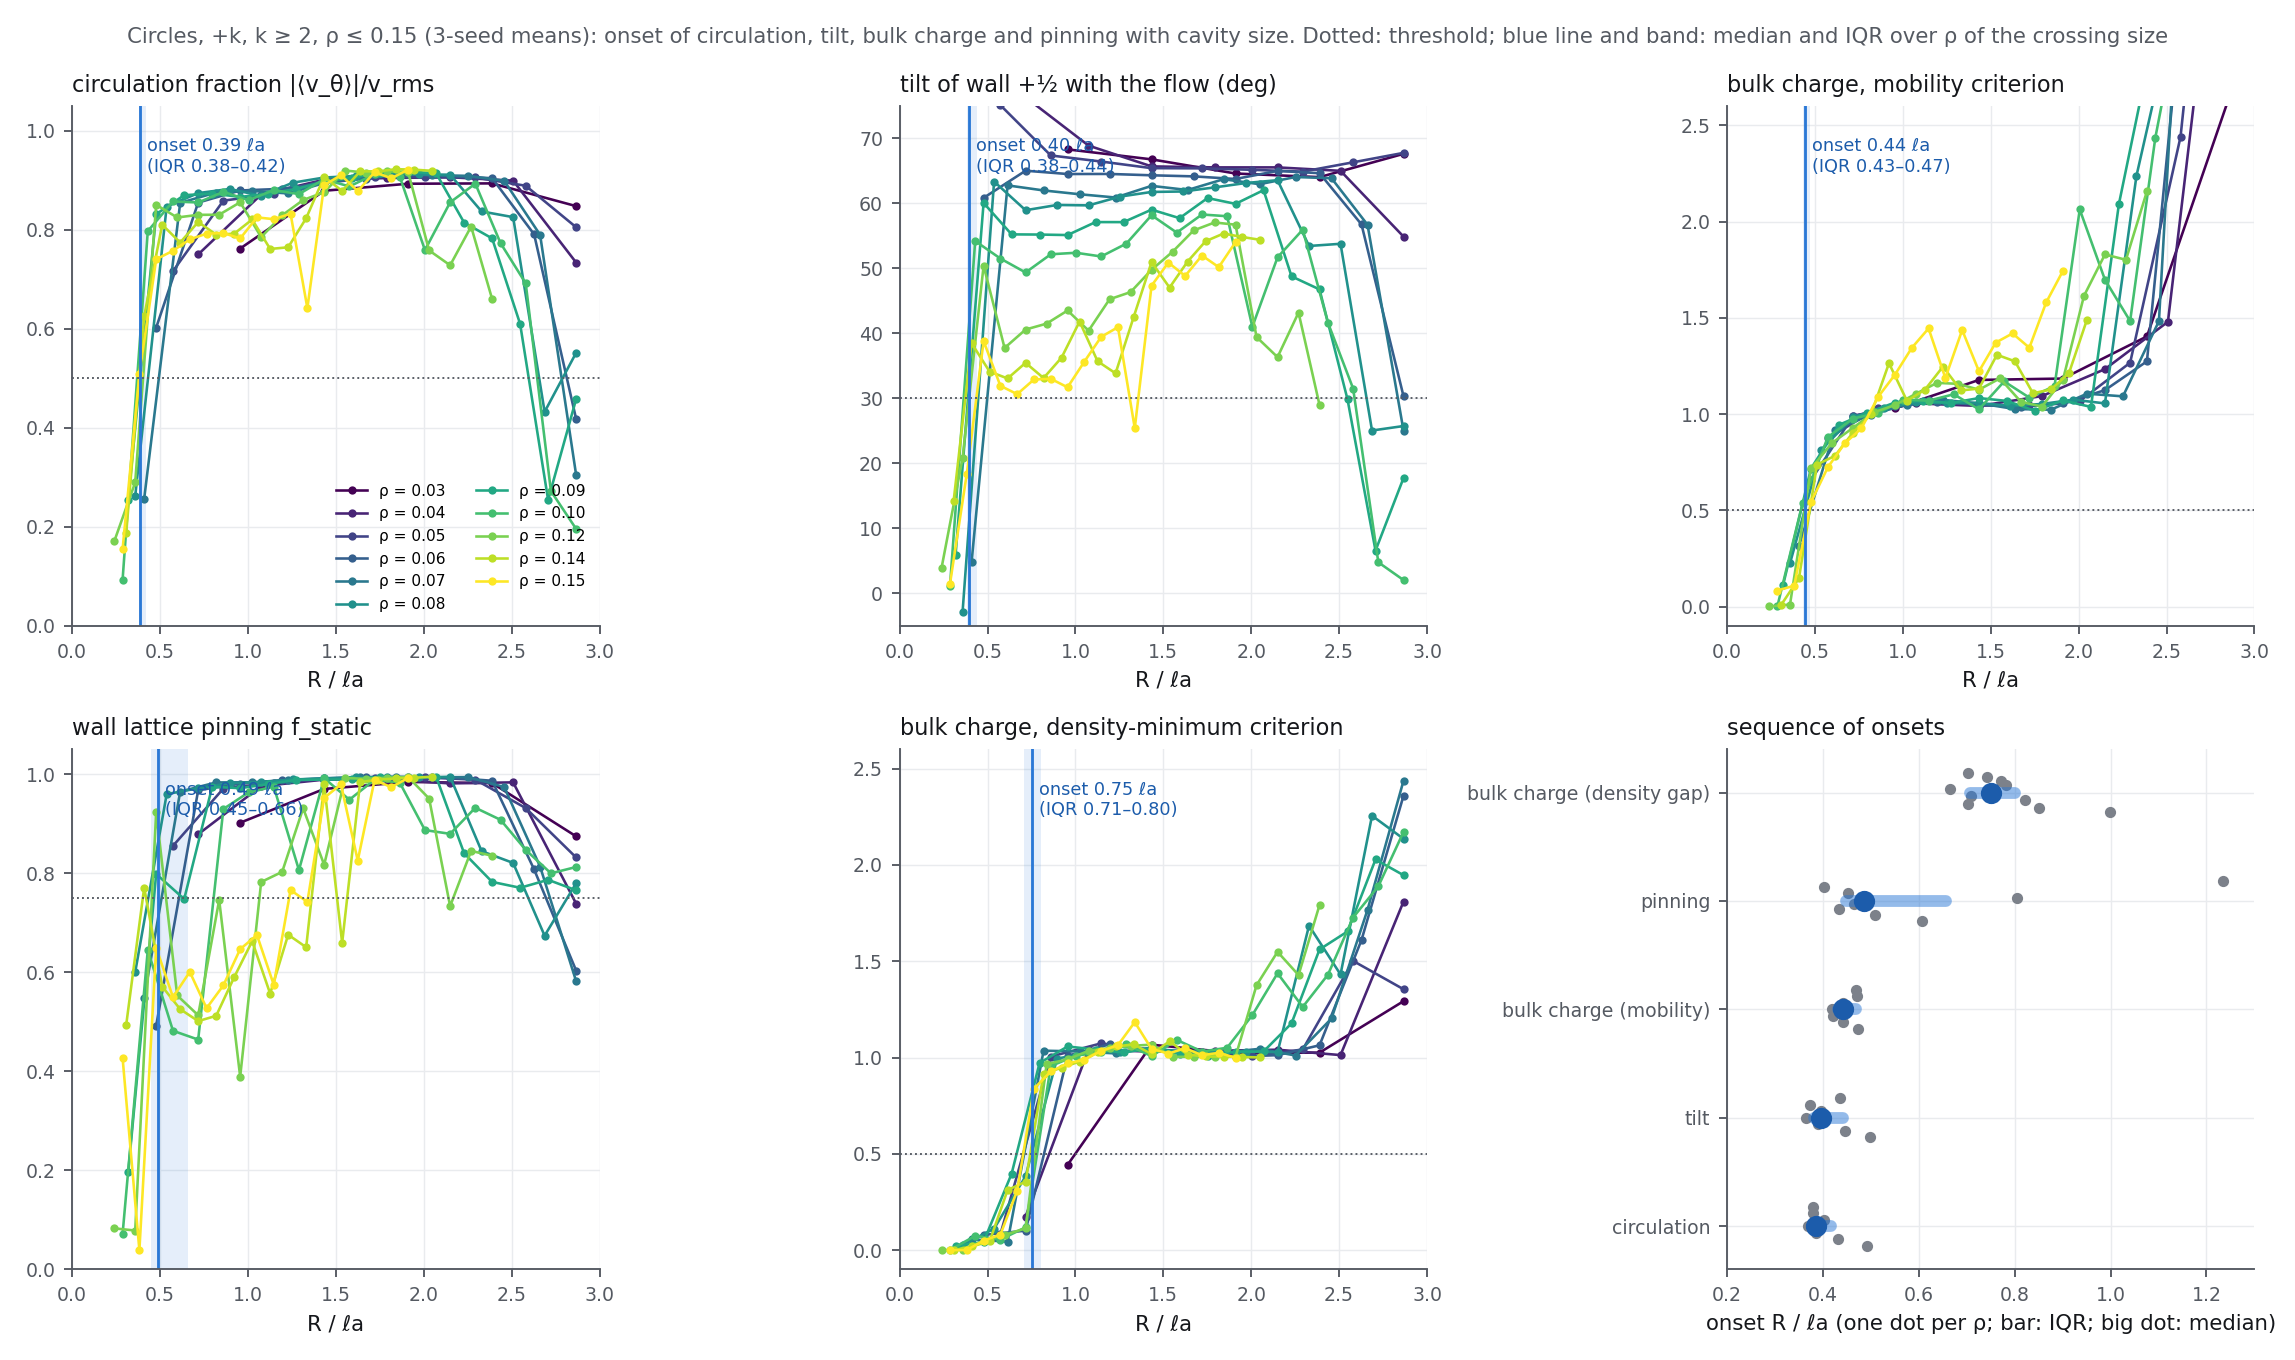
\includegraphics[width=\textwidth]{onset_circles.png}
\caption{\textbf{Onset of the layer/bulk structure in circles} ($+k$, $k\ge2$, $\rho\le0.15$, 3-seed means; one curve per $\rho$).
Circulation fraction $|\langle v_\theta\rangle|/v_\mathrm{rms}$, tilt of the wall $+\half$ signed with the flow, bulk charge from the mobility
criterion, static fraction of the wall lattice, and bulk charge from the density-minimum criterion, against $R/\la$. Dotted: threshold
(0.5, $30^\circ$, 0.5, 0.75, 0.5); blue line and band: median and interquartile range over $\rho$ of the size at which each curve first
crosses it. Last panel: the onsets in order, one dot per $\rho$. Onsets can only be measured for $\rho\ge0.07$, where the sweep has
cavities below $0.5\,\la$ with $k\ge2$.}\label{fig:onset}
\end{figure}
\begin{table}[H]\centering\small
\caption{Onset sizes $R/\la$ per density (\texttt{reports/master/data/onset\_circles.tsv}); ``--'': no crossing within the sweep.}\label{tab:onset}
\begin{tabular}{lccccc}\toprule
$\rho$ & circulation & tilt & bulk charge (mobility) & pinning & bulk charge (density gap)\\\midrule
0.07 & 0.49 & 0.50 & 0.47 & 0.51 & 0.71\\
0.08 & 0.43 & 0.45 & 0.44 & 0.43 & 0.75\\
0.09 & 0.39 & 0.39 & 0.42 & 0.47 & 0.67\\
0.10 & 0.37 & 0.37 & 0.42 & 0.81 & 0.78\\
0.12 & 0.40 & 0.40 & 0.44 & 0.45 & 0.77\\
0.14 & 0.38 & 0.37 & 0.47 & 0.40 & 0.74\\
0.15 & 0.38 & 0.44 & 0.47 & (1.23) & 0.70\\\midrule
median & \textbf{0.39} & \textbf{0.40} & \textbf{0.44} & 0.49 & 0.75\\\bottomrule
\end{tabular}
\end{table}
\begin{itemize}
  \item \textbf{The $+1$ bulk is born with the vortex.} Circulation, the downstream tilt of the wall $+\half$ and the bulk charge
        (mobility) switch on together at $R/\la\approx0.4$ (medians 0.39, 0.40, 0.44), for every density from 0.07 to 0.15. Below that
        size all $2k$ $+\half$ sit at the wall and there is no coherent vortex; above it two $+\half$ leave the wall and the cavity
        circulates. Pinning of the wall lattice follows (median 0.49, scattered), and the density gap between layer and bulk only forms
        at $\approx0.75\,\la$, which is why the density-minimum criterion lags.
  \item \textbf{The upper end mirrors it.} Above $\approx2.3$--$2.5\,\la$ the circulation fraction falls, the tilt vanishes and the bulk charge
        rises above 1 while the wall lattice stays mostly pinned but under-occupied: a \emph{less-charged layer}.
  \item \textbf{Relation to earlier work.} For a wall of charge $+1$, Norton et al.\ found that the onset of circulation occurs at a fixed
        value of $R\sqrt{\alpha}$, i.e.\ at fixed $R/\la$ \cite{TODO_Norton2018}; there the two $+\half$ already exist. Here the wall carries
        all $2k$ imposed $+\half$ below the onset, and the $+1$ bulk is created at the circulation onset, at the same $R/\la$ for every $k$ and
        $\rho$. This supports H4 directly: the bulk charge follows the vortex, at both ends of the size range (and in elongated cavities,
        where the vortex splits, Part~III).
\end{itemize}
\begin{figure}[H]\centering
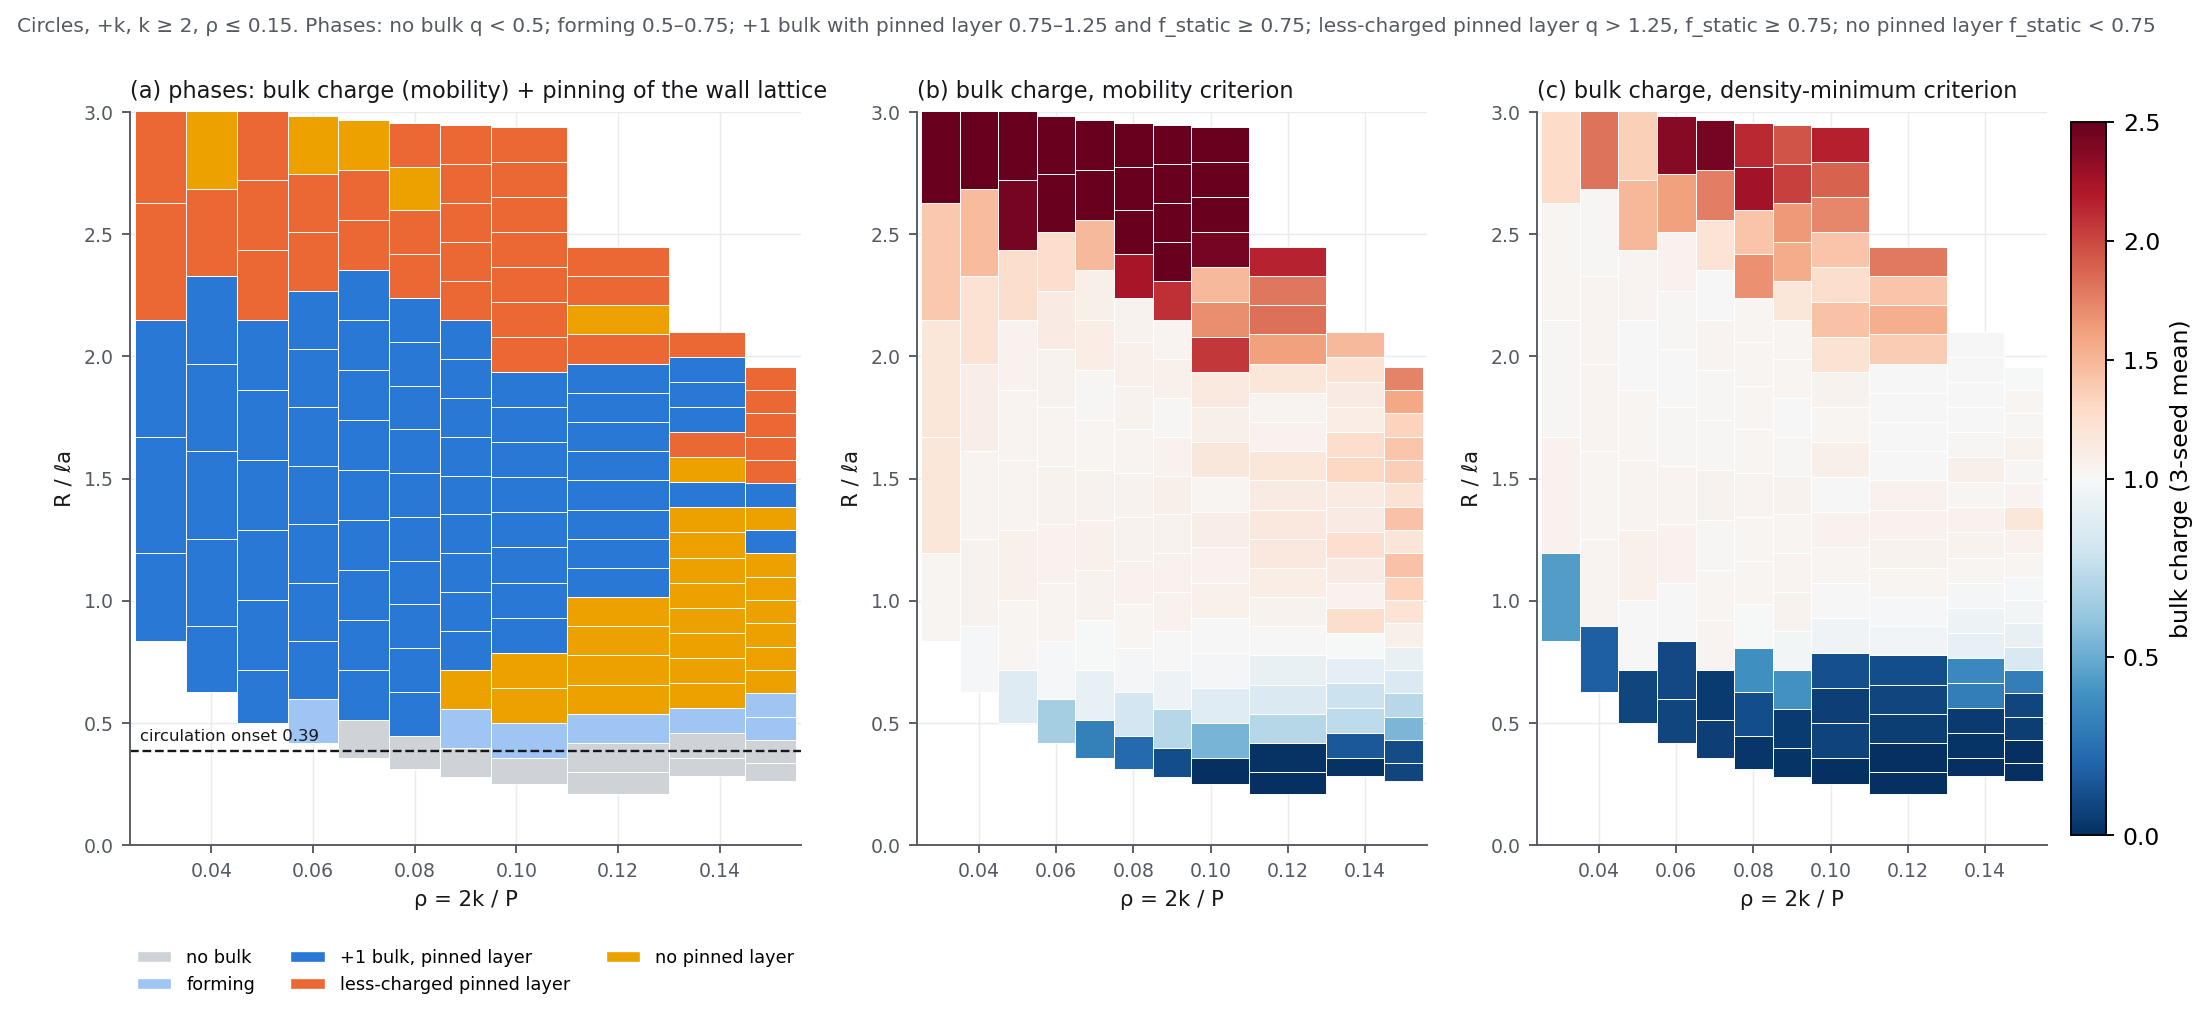
\includegraphics[width=\textwidth]{phase_circles.png}
\caption{\textbf{Phase diagram of circles} ($+k$, $k\ge2$, $\rho\le0.15$, 3-seed means). (a) Phases from the mobility bulk charge $q$
and the static fraction $f_\mathrm{static}$ of the wall lattice: no bulk ($q<0.5$); forming ($0.5\le q<0.75$); $+1$ bulk with a pinned layer
($0.75\le q\le1.25$, $f_\mathrm{static}\ge0.75$); less-charged pinned layer ($q>1.25$, $f_\mathrm{static}\ge0.75$); no pinned layer
($f_\mathrm{static}<0.75$). Dashed: median circulation onset. (b) Bulk charge from the mobility criterion; (c) from the density-minimum
criterion (cross-check), colour centred on 1.}\label{fig:phase}
\end{figure}
\begin{itemize}
  \item 71 of 151 points are $+1$ bulk with a pinned layer, 35 less-charged pinned layer (large $R$), 28 no pinned layer, 17 no bulk or forming.
  \item \textbf{A band without pinning at high density:} for $\rho\ge0.10$ and $R\approx0.5$--$1.4\,\la$ the bulk charge is $\approx1$ but the
        crowded wall lattice keeps rearranging ($f_\mathrm{static}<0.75$; rearrangement times 100--1000, Sec.~\ref{sec:clattice}). Whether this
        is physical or due to the anchoring approaching its resolution limit ($\rho\to0.15$) is open.
  \item The mobility bulk charge sits slightly above 1 (1.05--1.2) inside the $+1$ region, the known bias of this criterion
        (occurrences on broken tracks are skipped; Appendix~\ref{app:issues}); the density-minimum criterion gives 1.00--1.05 there.
\end{itemize}

\subsection{Six bulk-charge criteria over the whole sweep}\label{sec:criteria}
Figures~\ref{fig:critmaps}--\ref{fig:transitions} compare the criteria of Sec.~\ref{sec:edge} on 930 runs ($\rho\le0.15$, both
signs, means over 3 seeds).
\begin{figure}[H]\centering
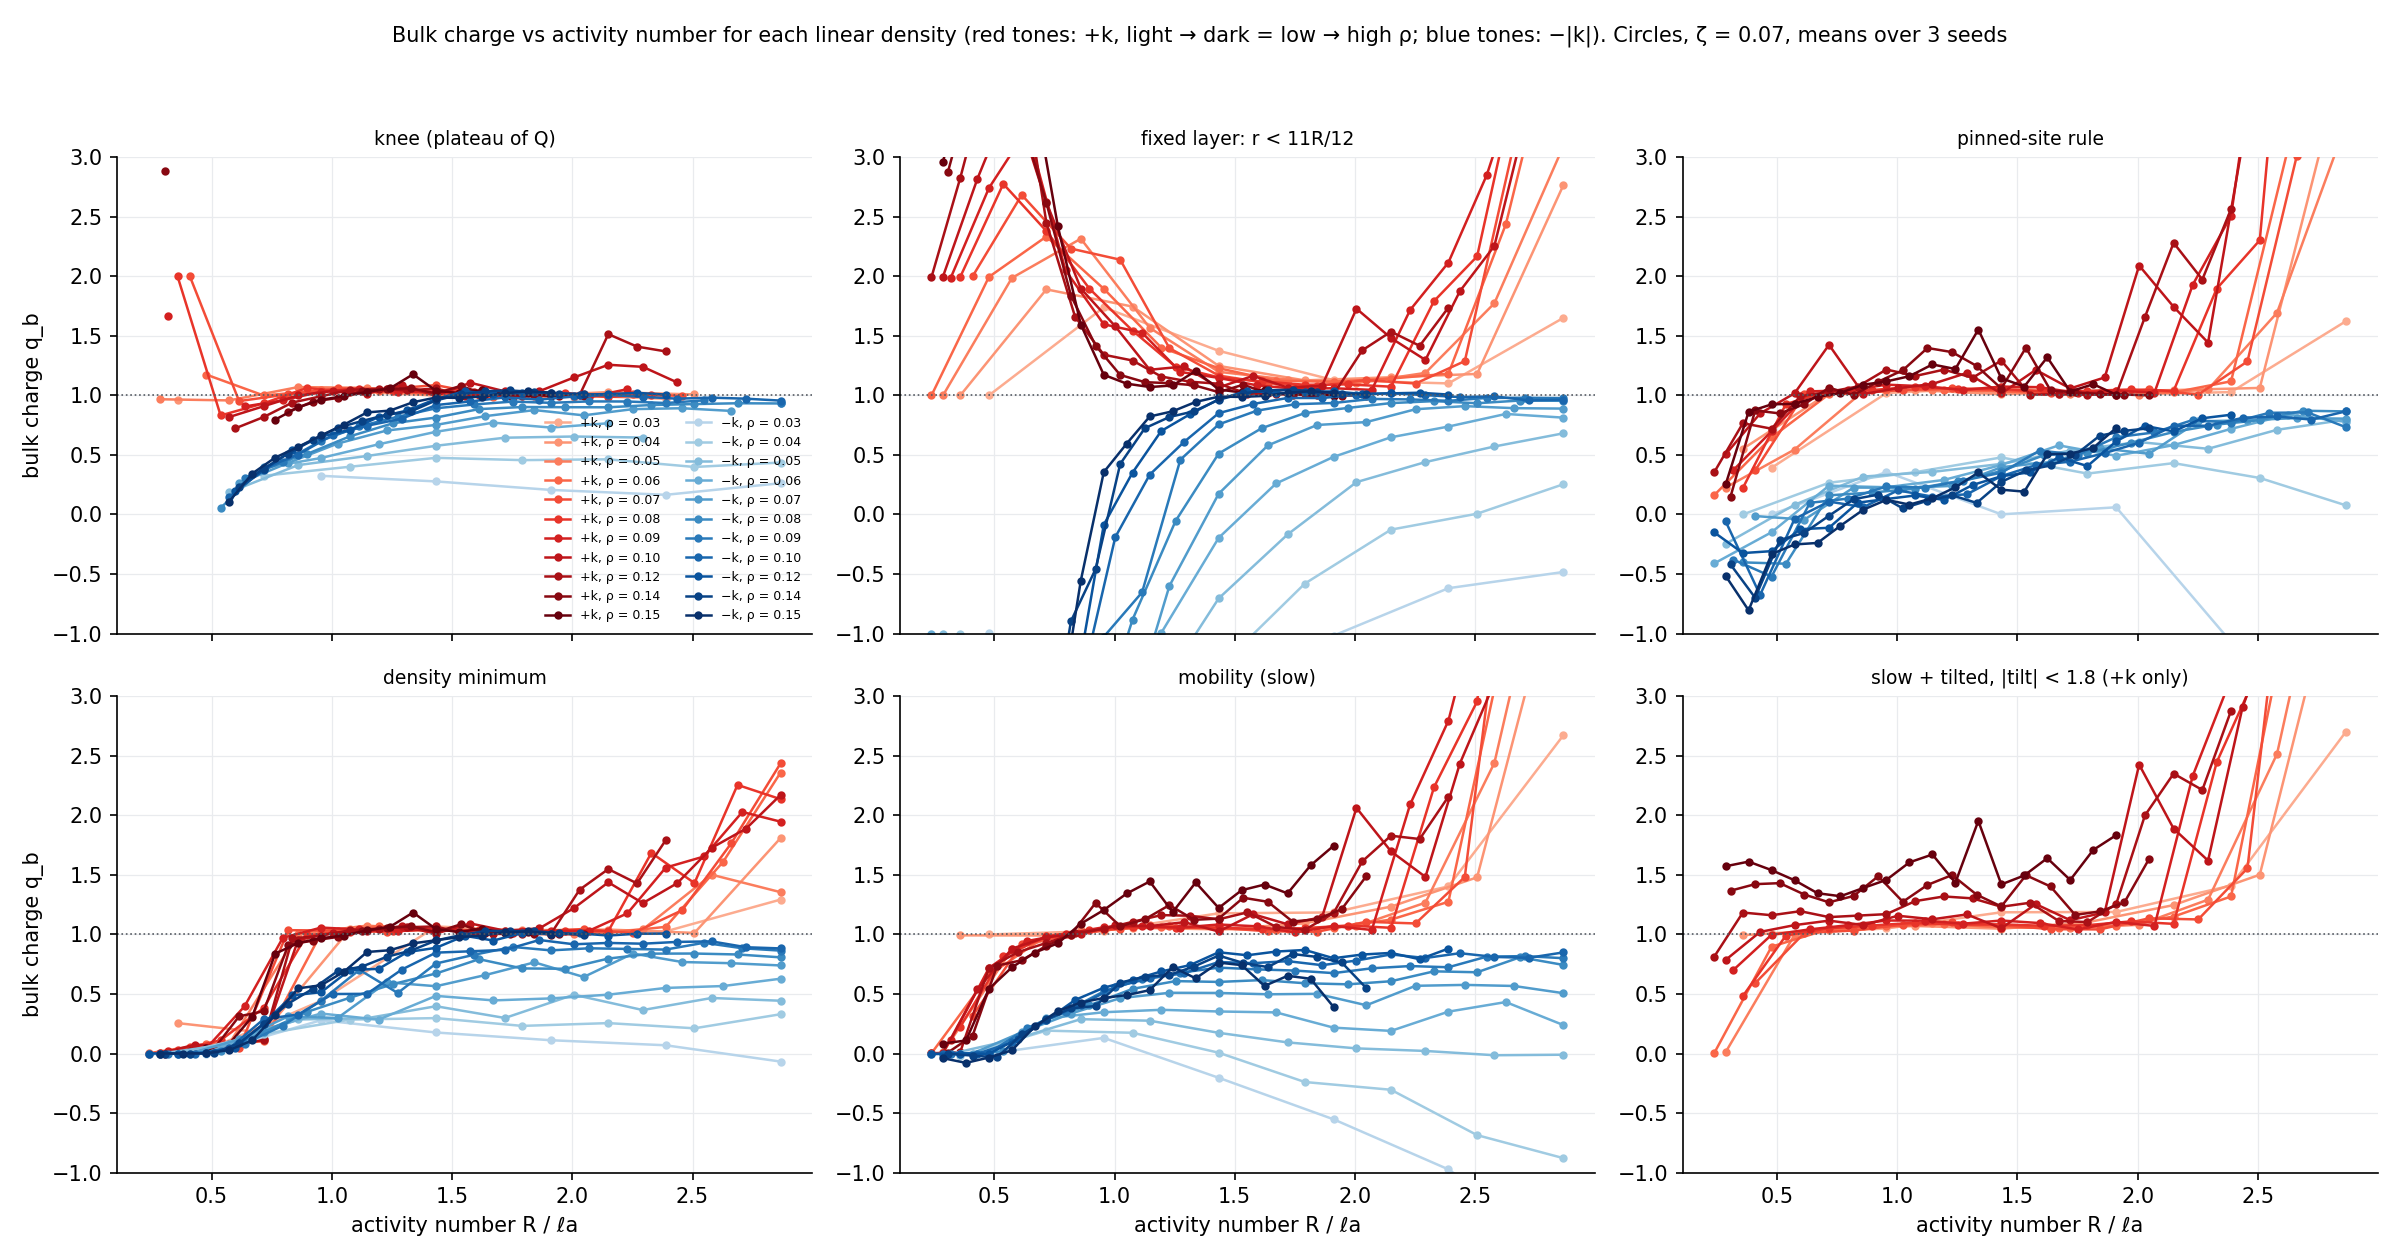
\includegraphics[width=\textwidth]{crit_bulk_vs_R.png}
\caption{Bulk charge against $R/\la$ for six criteria; red tones $+k$ (light to dark: low to high $\rho$), blue tones $-|k|$.}\label{fig:critR}
\end{figure}
\begin{figure}[H]\centering
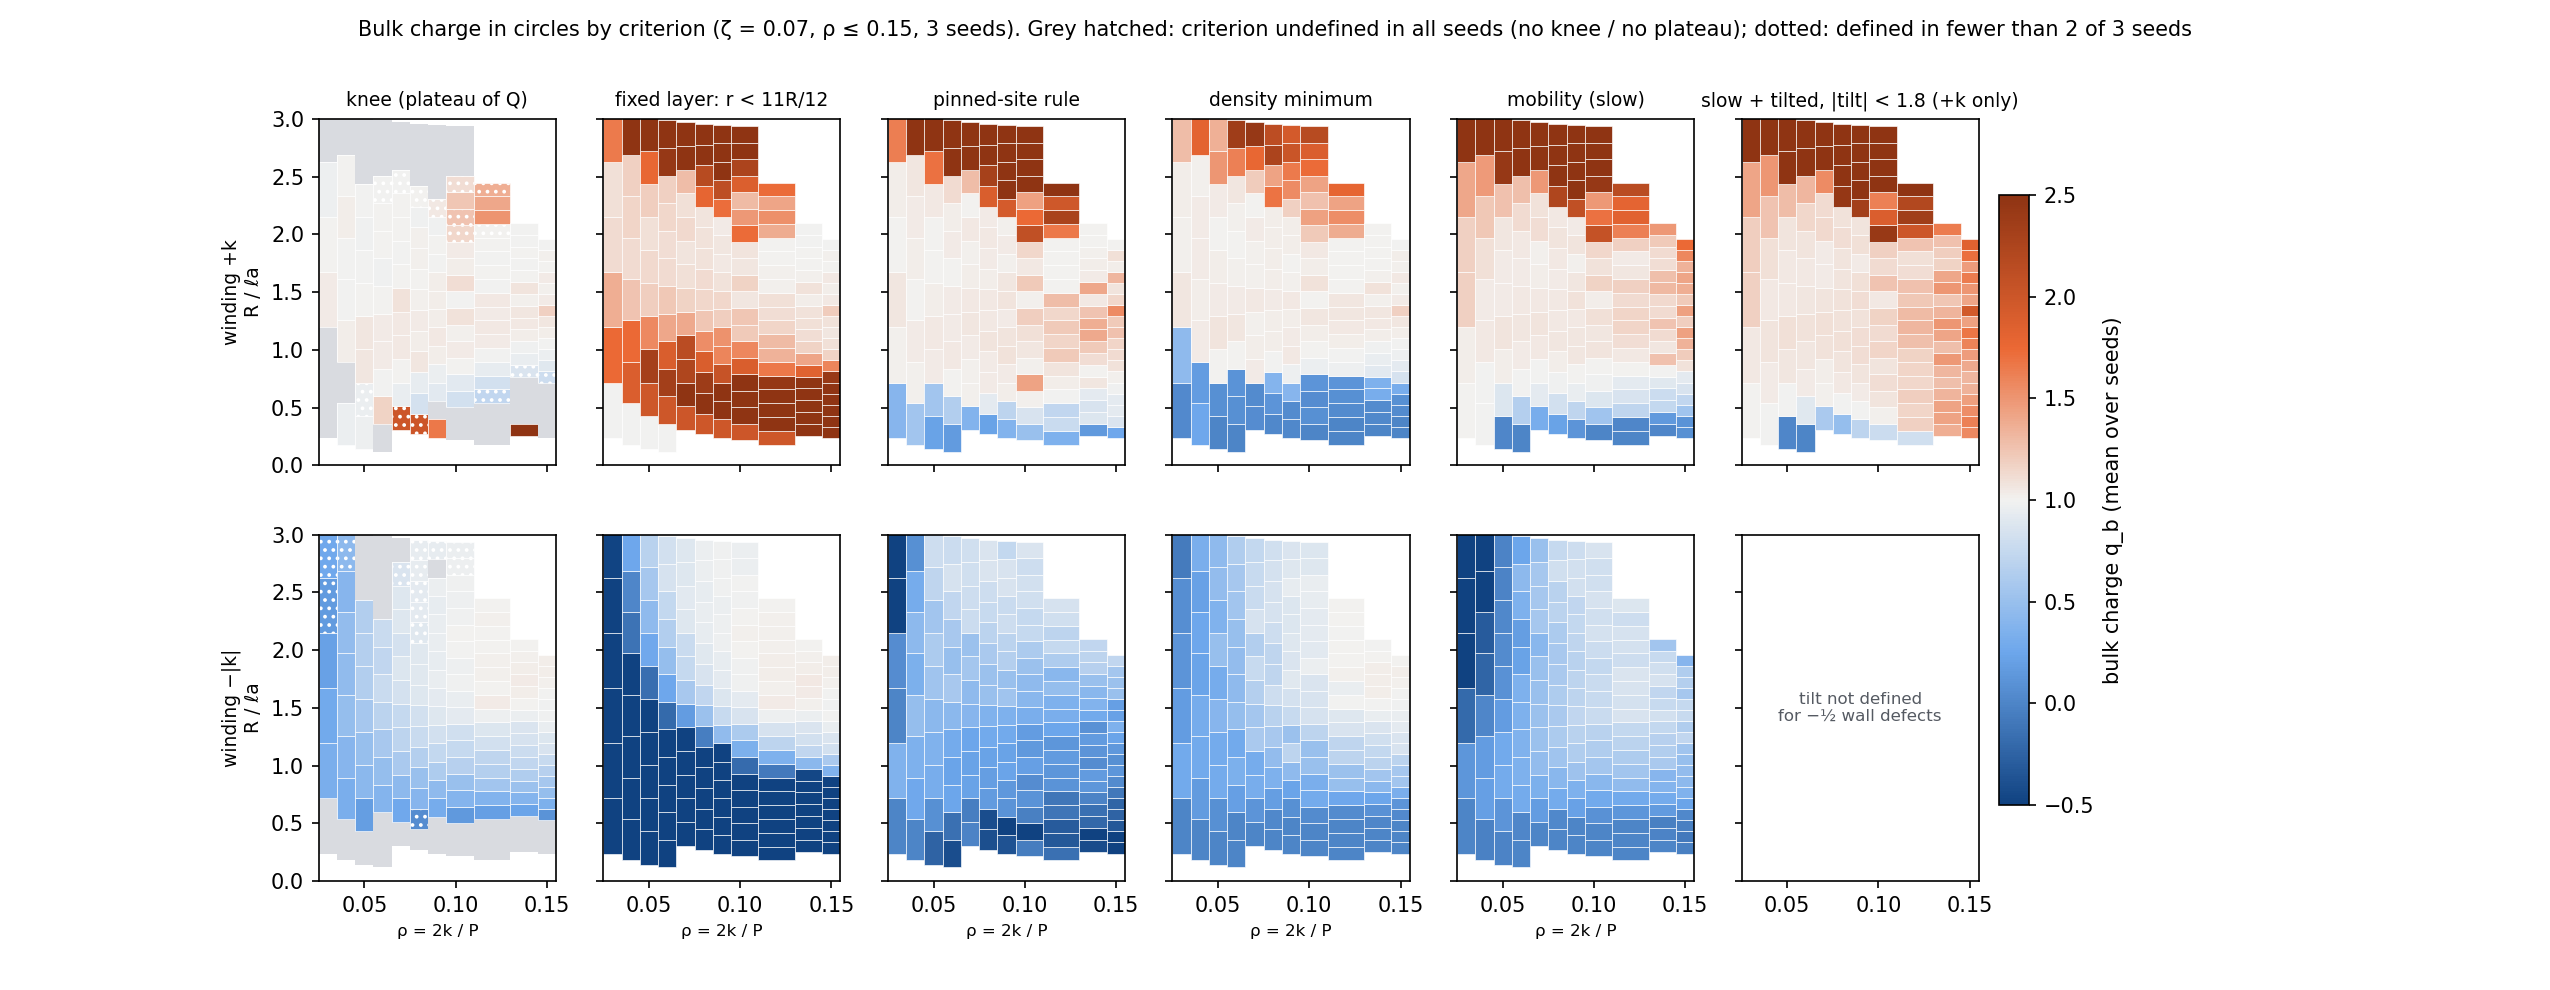
\includegraphics[width=\textwidth]{crit_bulk_maps.png}
\caption{The same as maps over $(\rho,R/\la)$; top $+k$, bottom $-|k|$. Grey hatched: criterion undefined in all seeds (no
knee); dotted: defined in fewer than 2 of 3 seeds.}\label{fig:critmaps}
\end{figure}
\begin{figure}[H]\centering
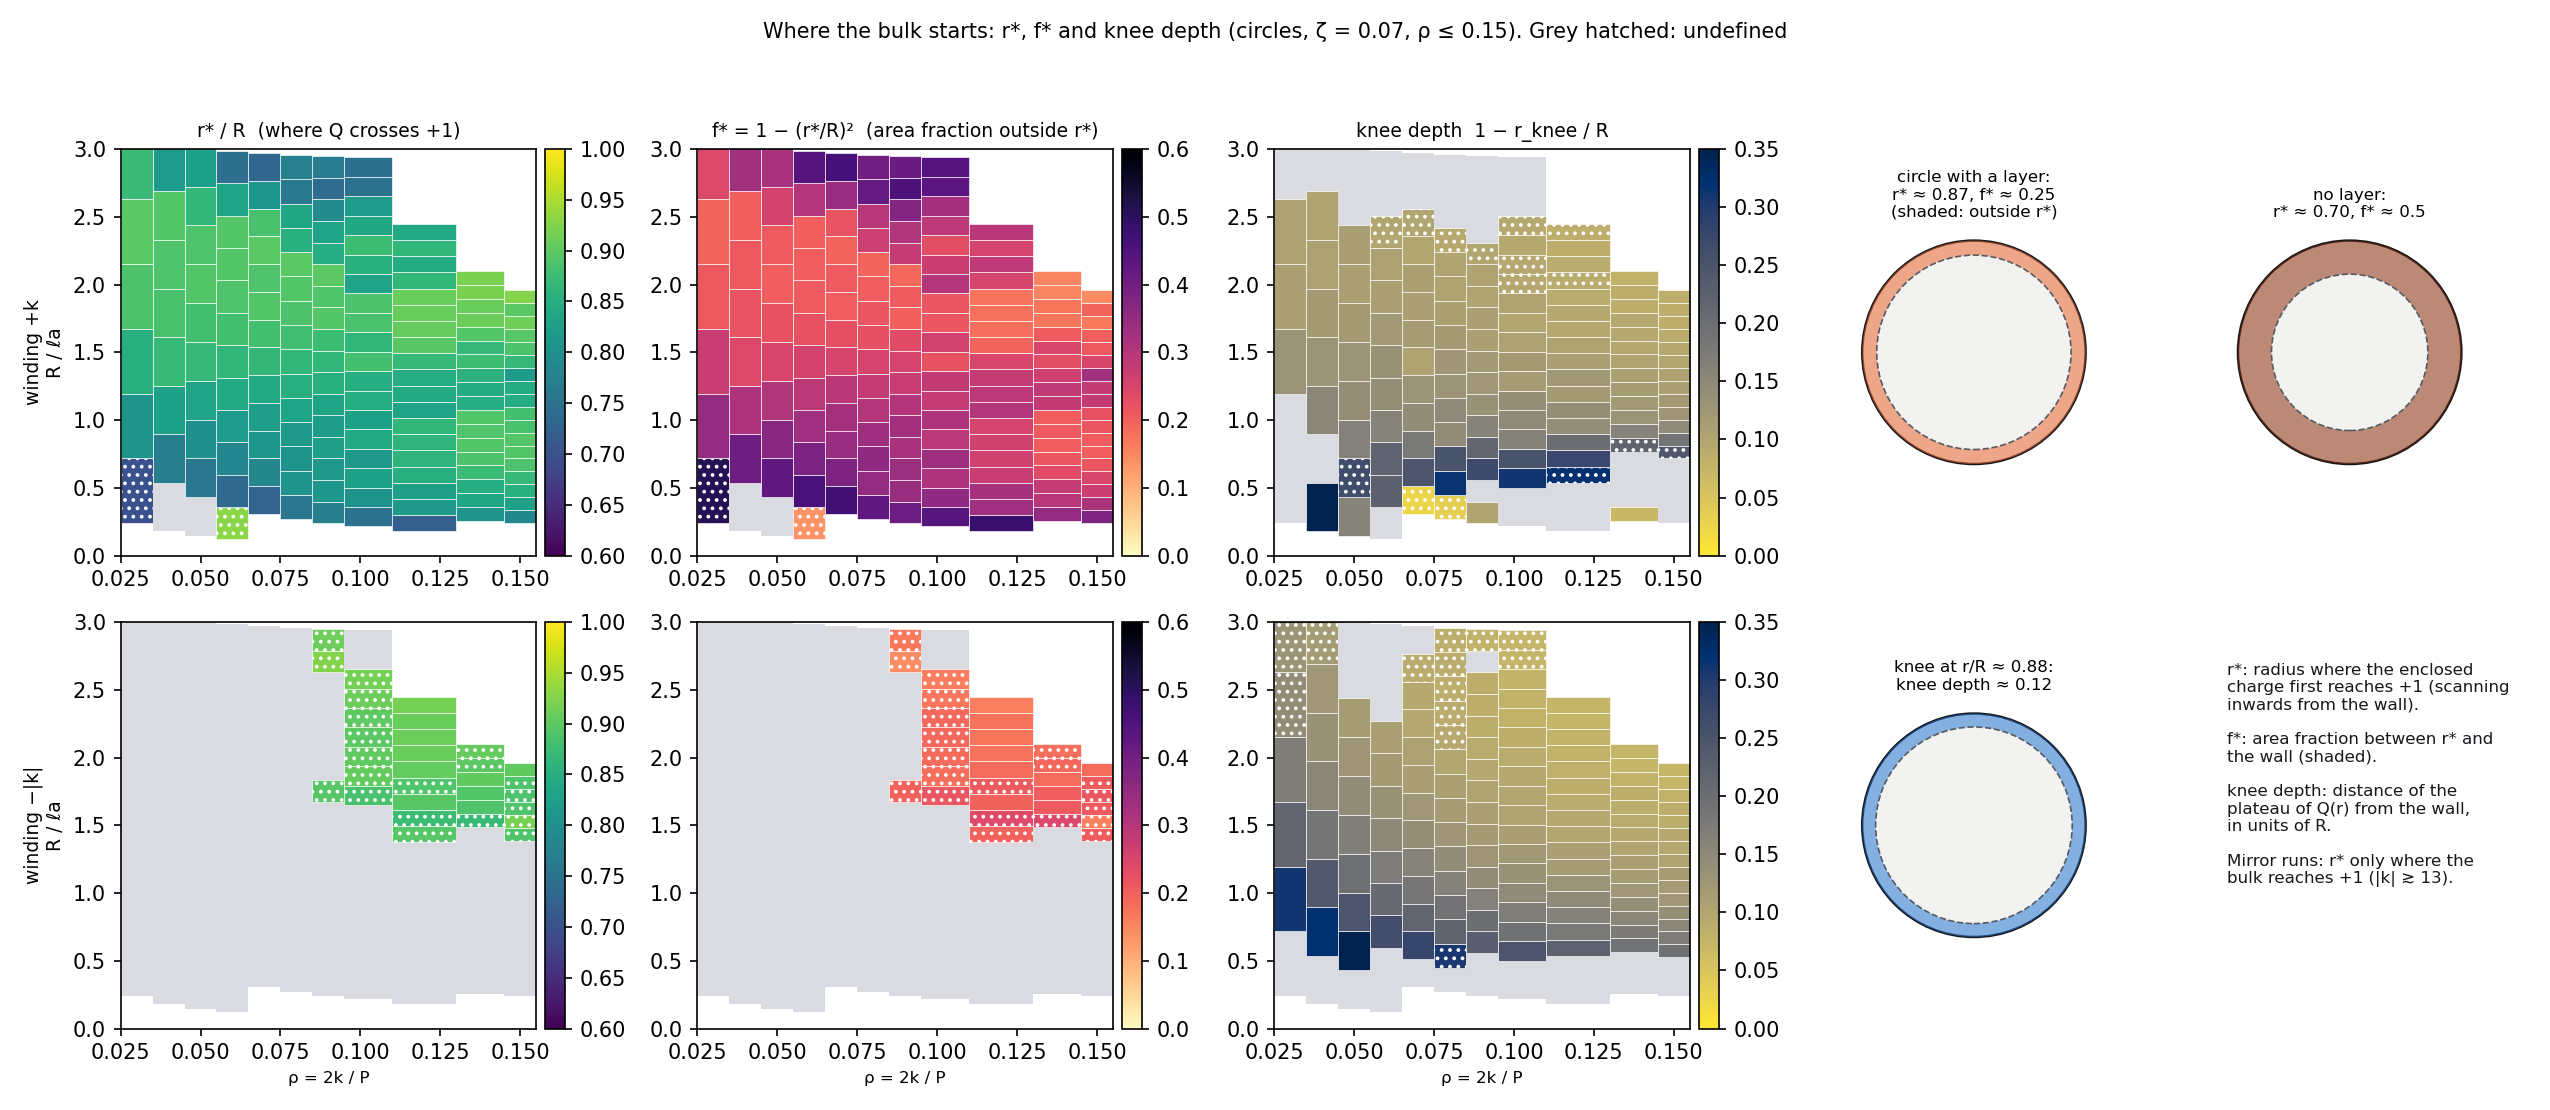
\includegraphics[width=\textwidth]{crit_rstar_fstar_knee.png}
\caption{Where the bulk starts: $r^*/R$ (outermost $Q=+1$ crossing), $f^*=1-(r^*/R)^2$ and the knee depth $1-r_\mathrm{knee}/R$;
top $+k$, bottom $-|k|$ (for $-|k|$, $r^*$ exists only where the bulk reaches $+1$).}\label{fig:rstar}
\end{figure}
\begin{figure}[H]\centering
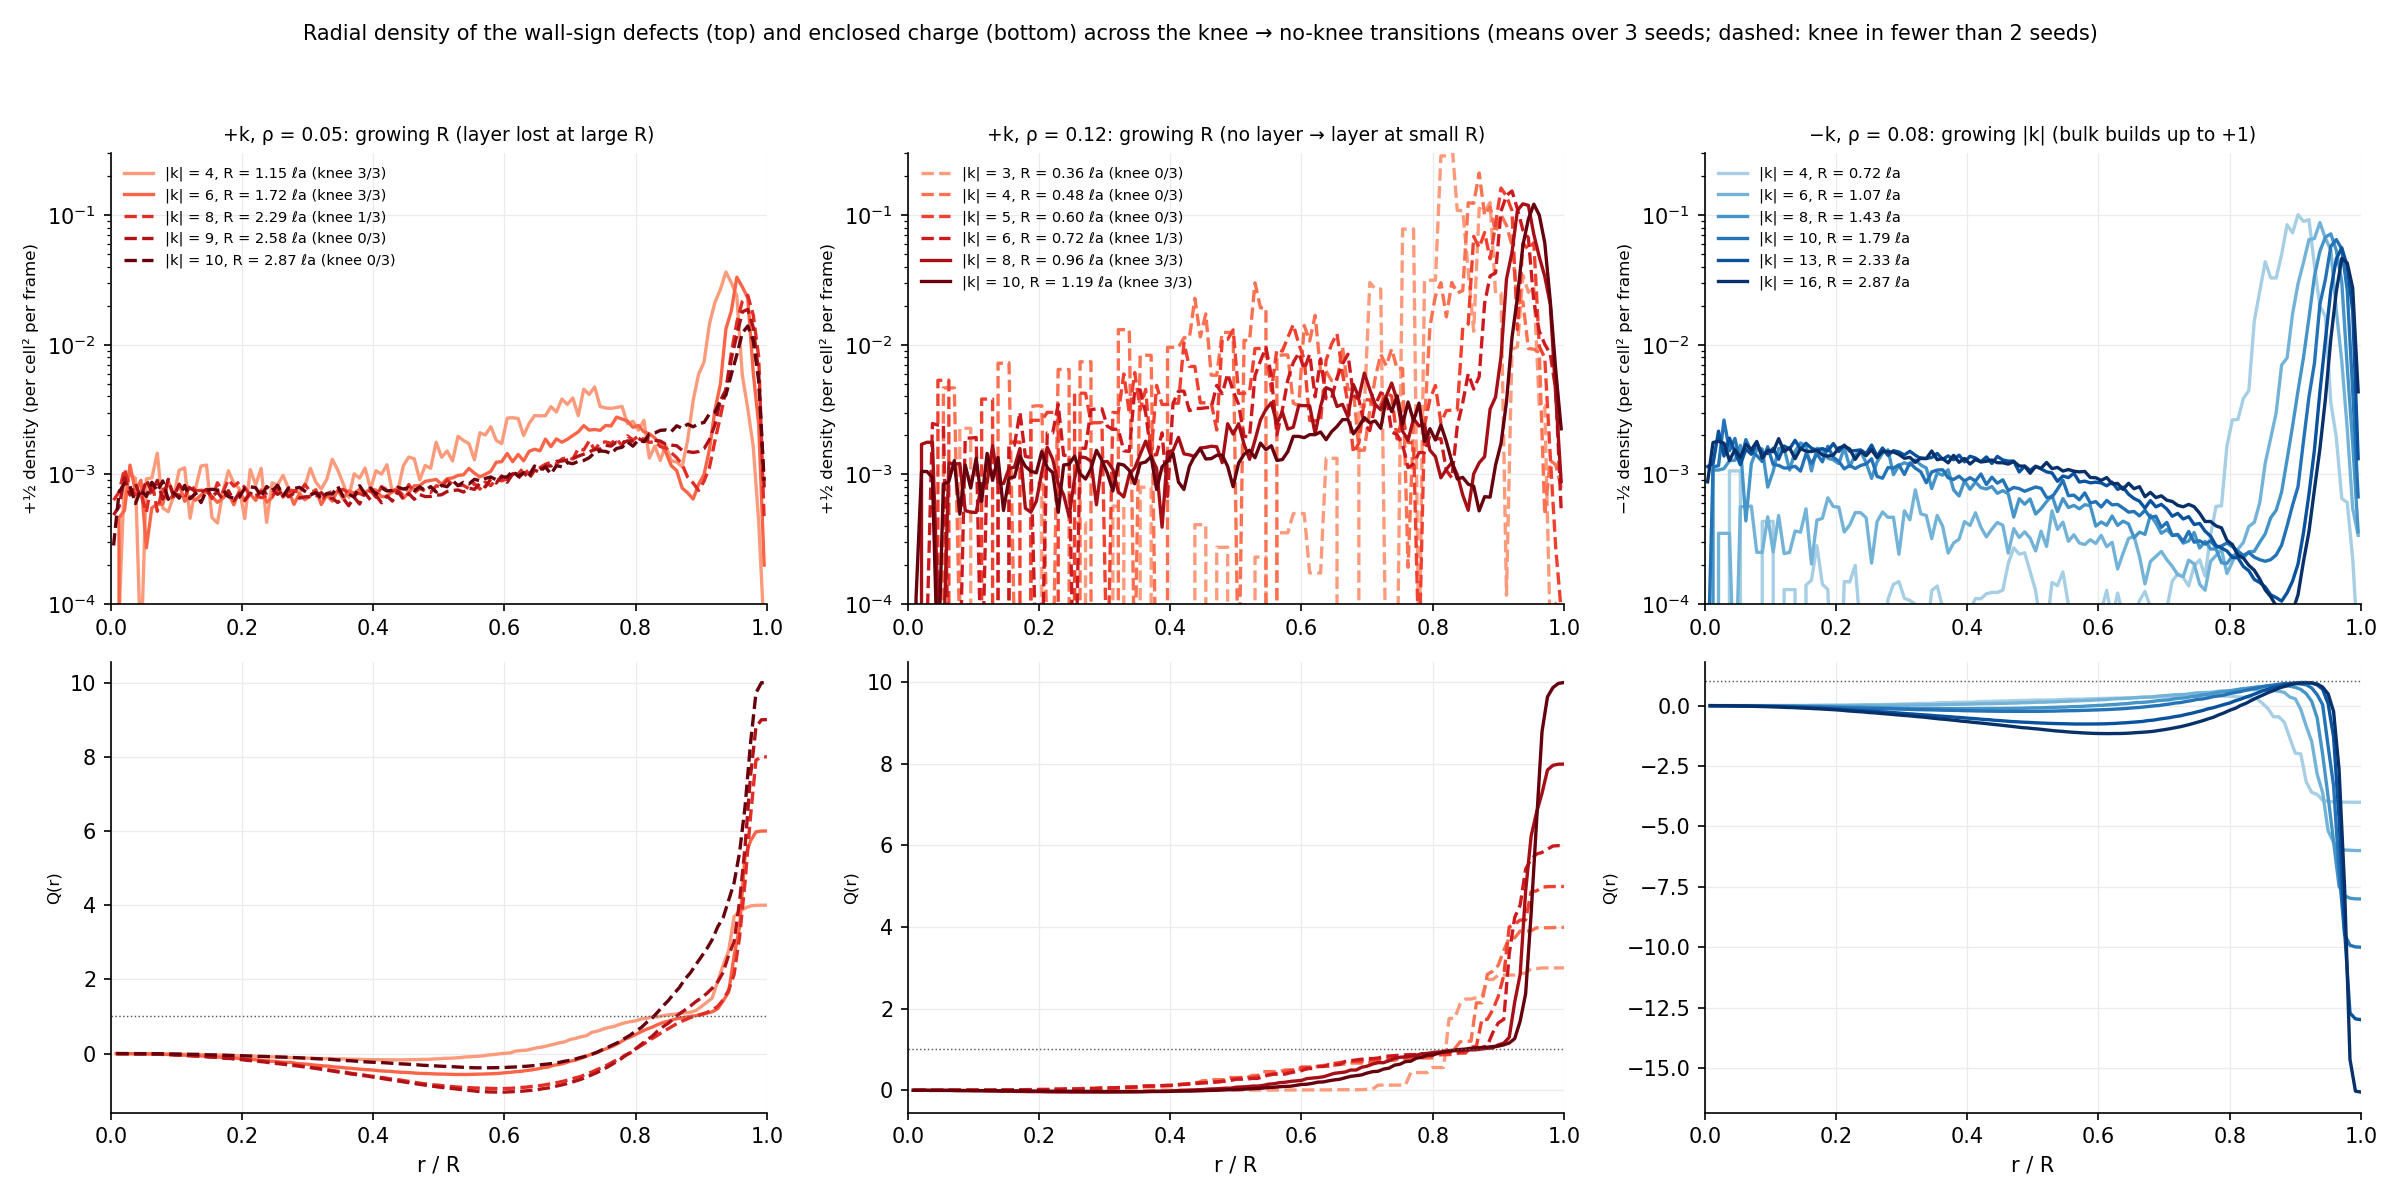
\includegraphics[width=\textwidth]{crit_transitions.png}
\caption{Radial density of the wall-sign defects (top) and $Q(r)$ (bottom) across the knee $\to$ no-knee transitions: $+k$ at
$\rho=0.05$ with growing $R$ (layer lost at large $R$), $+k$ at $\rho=0.12$ (layer appears from $\approx0.96\,\la$), $-k$ at
$\rho=0.08$ with growing $|k|$ (bulk builds up to $+1$). Dashed: knee in fewer than 2 seeds.}\label{fig:transitions}
\end{figure}
\begin{itemize}
  \item \textbf{$+k$:} all criteria agree on $q_b\approx1$ for $R\approx0.8$--$2\,\la$ at every $\rho$. The knee is the most
        robust ($\approx1$ from $\approx0.6$ to $2.4\,\la$) but undefined at large $R$ and low $\rho$. The fixed-depth cut
        ($r<11R/12$) fails at small $R$ (layer thicker than $R/12$: $q_b\gg1$ below $\approx1\,\la$) and at large $R$. Density
        minimum and mobility give $q_b\to0$ below 0.6--0.8\,$\la$ (no bulk defects there). Above 2--2.5\,$\la$ all criteria
        except the knee rise above 1 (defects leave the layer), earliest at high $\rho$. Slow + tilted overcounts (1.3--1.6) at
        high $\rho$, where the wall tilt is smaller (Sec.~\ref{sec:cflow}).
  \item \textbf{$-|k|$:} the knee value rises with $\rho$ and $R$ (0.3--0.5 at $\rho\le0.05$, 0.9--1 only for $\rho\gtrsim0.10$
        and $R\gtrsim1.5\,\la$); site rule and mobility saturate near 0.8 (Sec.~\ref{sec:mirror}).
  \item \textbf{Choice for the paper:} the knee of $Q(r)$ as the primary bulk-charge measure, the density minimum and the
        mobility as cross-checks; no fixed-depth cut.
\end{itemize}

%=====================================================================
\section{Negative winding: the bulk stays positive}\label{sec:mirror}
With winding $-|k|$ the wall must carry at least $2|k|$ $-\half$ defects. $-\half$ defects do not self-propel, so a positive bulk
cannot come from wall defects swimming off; and the excess over the natural $+1$ of a homeotropic disc is $-(|k|+1)$, not
$k-1$, so the two signs are not mirror images even topologically. Data: 570 active runs ($\rho\le0.15$, 3 seeds), same
grid and outputs as the positive sweep. Bulk charge = height of the positive peak of $Q(r)$ before the plunge to $-|k|$
(Sec.~\ref{sec:methods-knee}).
\begin{figure}[H]\centering
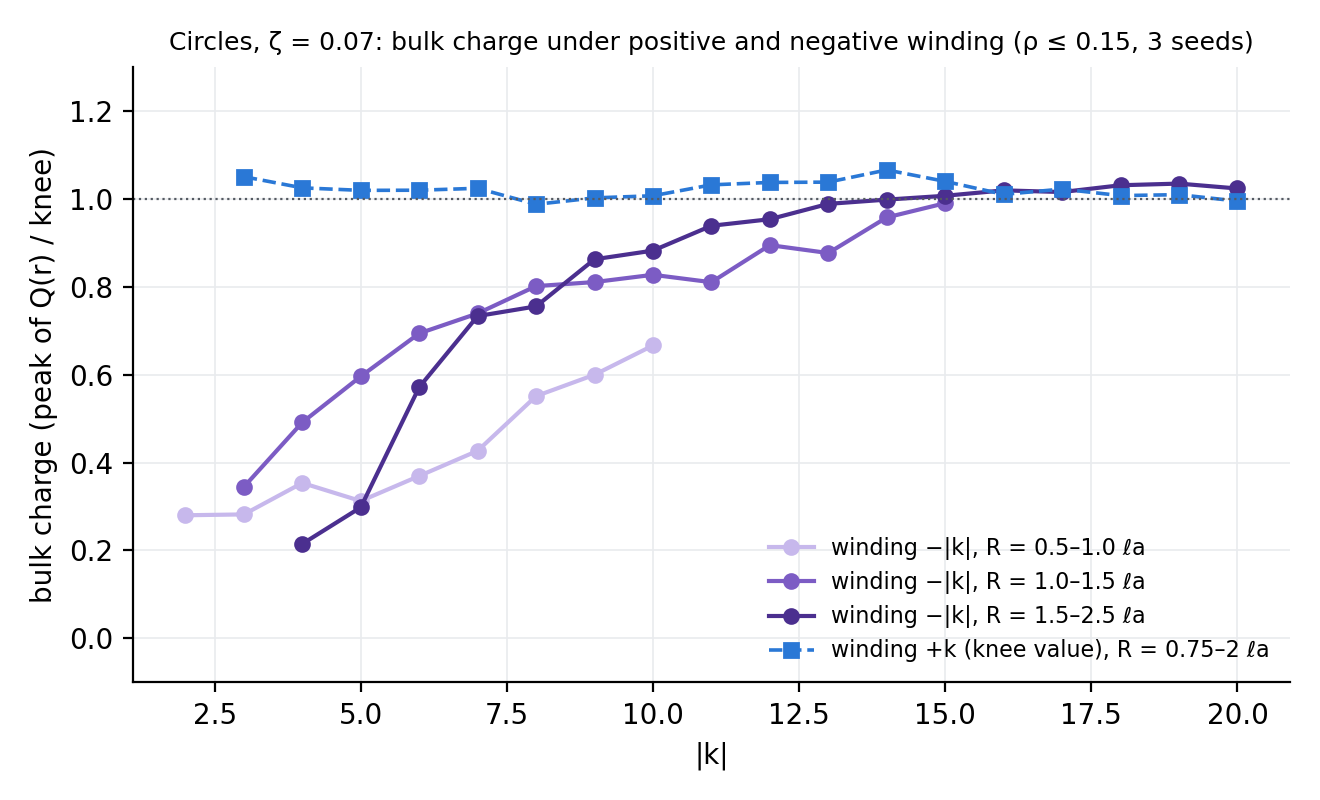
\includegraphics[width=0.78\textwidth]{mirror_bulk_vs_k.png}
\caption{Bulk charge against $|k|$: positive winding (knee value) and negative winding (peak of $Q(r)$), $\rho\le0.15$.}\label{fig:mirror}
\end{figure}
\begin{figure}[H]\centering
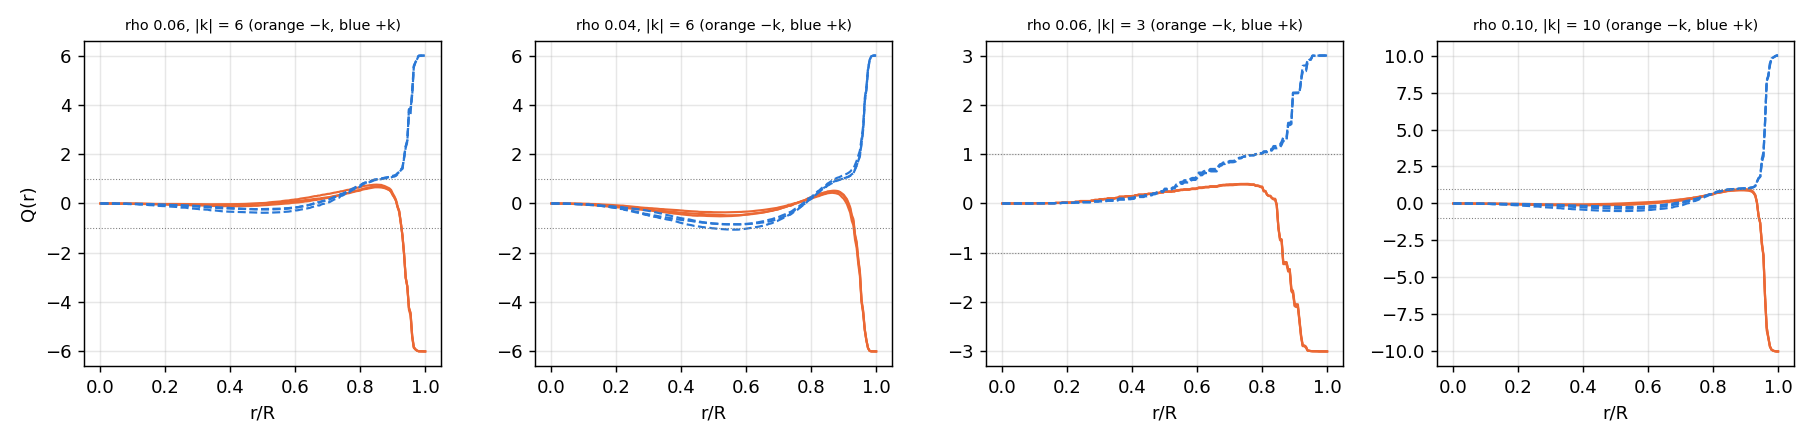
\includegraphics[width=0.85\textwidth]{mirror_Q_check.png}
\caption{Examples of $Q(r)$ with negative winding: a positive peak inside, then the plunge to $-|k|$ at the wall.}\label{fig:mirrorQ}
\end{figure}
\begin{table}[H]\centering\small
\caption{Mirror runs: mean peak $Q$ (bulk charge) over $\rho$ and seeds, and wall $-\half$ per frame; $2|k|$ = forced,
$2|k|+2$ = what a $+1$ bulk needs.}\label{tab:mirror}
\begin{adjustbox}{max width=\textwidth}
\begin{tabular}{rcccc|rcccc}\toprule
$|k|$ & bulk & range & wall $-\half$ & ($2|k|$, $2|k|+2$) & $|k|$ & bulk & range & wall $-\half$ & ($2|k|$, $2|k|+2$)\\\midrule
2 & 0.09 & 0.00--0.34 & 3.78 & (4, 6) & 12 & 0.92 & 0.82--1.02 & 25.20 & (24, 26)\\
4 & 0.27 & 0.00--0.52 & 7.83 & (8, 10) & 14 & 0.96 & 0.85--1.03 & 29.46 & (28, 30)\\
6 & 0.47 & 0.00--0.76 & 11.71 & (12, 14) & 15 & 1.00 & 0.94--1.08 & 31.74 & (30, 32)\\
8 & 0.68 & 0.42--0.88 & 16.28 & (16, 18) & 17 & 1.01 & 0.97--1.06 & 35.86 & (34, 36)\\
10 & 0.83 & 0.61--0.97 & 20.80 & (20, 22) & 20 & 1.01 & 0.96--1.05 & 41.91 & (40, 42)\\\bottomrule
\end{tabular}
\end{adjustbox}
\end{table}
\begin{table}[H]\centering\small
\caption{Mirror runs: mean bulk charge by $|k|$ (rows) and $R/\la$ (columns), $\rho\le0.15$.}\label{tab:mirror2}
\begin{adjustbox}{max width=\textwidth}
\begin{tabular}{lcccccc}\toprule
$|k|$ & 0.50--0.75 & 0.75--1.00 & 1.00--1.50 & 1.50--2.00 & 2.00--2.50 & 2.50--3.00\\\midrule
1--2 & 0.26 & 0.33 & & & & \\
3--4 & 0.26 & 0.44 & 0.42 & 0.21 & & \\
5--6 & 0.22 & 0.52 & 0.64 & 0.57 & 0.30 & 0.10\\
7--9 & 0.37 & 0.57 & 0.78 & 0.83 & 0.71 & 0.55\\
10--12 & & 0.67 & 0.84 & 0.95 & 0.89 & 0.83\\
13--16 & & & 0.93 & 1.02 & 0.98 & 0.94\\\bottomrule
\end{tabular}
\end{adjustbox}
\end{table}
\begin{itemize}
  \item \textbf{The bulk charge is positive, not $-1$,} and grows with $|k|$: 0.09 ($|k|=2$), 0.47 (6), 0.83 (10), 1.0 from
        $|k|\approx15$. The wall carries $\approx2|k|+2q_b$ $-\half$, i.e.\ each unit of bulk charge corresponds to two extra $-\half$
        absorbed at the wall, whose $+\half$ partners form the bulk.
  \item At fixed size the bulk charge rises with $|k|$; at fixed $|k|$ it peaks at $R\approx1.5$--$2\,\la$ and falls for larger
        cavities.
  \item \textbf{Reading:} $+1$, the Euler characteristic of the disc, is the attractor for both winding signs, but activity breaks
        the mirror symmetry. With $+k$ the $+1$ bulk appears at every $k\ge2$, made of self-propelled $+\half$ that leave the
        wall. With $-k$ the wall has to absorb two extra $-\half$, which happens fully only when the wall is crowded
        ($|k|\gtrsim13$--15).
  \item \textbf{Where the missing charge is} (Sec.~\ref{sec:clattice}): the $-\half$ wall lattice already has the period of a
        $+1$ bulk ($2|k|+2$ sites) but only 70--90\% of the sites are occupied at low $\rho$; the bulk charge computed from the
        wall count tracks the slow-defect criterion ($r=0.96$; median difference to the density criterion 0.05).
  \item Passive mirror runs are exact mirrors (bulk 0), so the asymmetry is entirely active.
\end{itemize}

\subsection{Is the edge shielded? Encounters between bulk and wall defects}\label{sec:shield}
The wall layer is expected to screen the attraction between itself and opposite-sign bulk defects (elastic shielding by an evenly
distributed charged layer; B.~Loewe). In the mirror circles this matters most: bulk $+\half$ are motile and reach the wall, where the
$-\half$ lattice sits. Test (\texttt{reports/master/scripts/shielding\_test.py}, method in Sec.~\ref{sec:m-shield}): every first approach
of a mobile defect to within 4 cells of an opposite-sign defect is an encounter; it ends in annihilation if both tracks end within 10 time
units of each other, at most 4 cells apart. Encounters with wall targets ($s<4$ cells) are compared with encounters with bulk targets
($s>6$) in the same runs. Circles with $\rho=0.05$--0.12, $R=1.0$--$2.3\,\la$, $|k|\ge2$, 3 seeds (114 runs per sign).
\begin{table}[H]\centering\small
\caption{Encounters and annihilation probabilities (pooled; $\pm$: binomial standard error). Close: encounters whose closest approach
within the next 20 time units is $\le2$ cells.}\label{tab:shield}
\begin{adjustbox}{max width=\textwidth}
\begin{tabular}{llcccc}\toprule
winding & mobile defect meets & encounters & $P$(annihilation) & close encounters (fraction) & $P$(annihilation | close)\\\midrule
$-k$ & wall $-\half$ & 41\,708 & $0.218\pm0.002$ & 11\,731 (0.28) & $0.460\pm0.005$\\
     & bulk $-\half$ & 69\,989 & $0.534\pm0.002$ & 40\,199 (0.57) & $0.568\pm0.002$\\
$+k$ & wall $+\half$ & 2\,635 & $0.308\pm0.009$ & 1\,197 (0.45) & $0.410\pm0.014$\\
     & bulk $+\half$ & 78\,007 & $0.523\pm0.002$ & 46\,545 (0.60) & $0.562\pm0.002$\\\bottomrule
\end{tabular}
\end{adjustbox}
\end{table}
\begin{itemize}
  \item \textbf{Negative winding:} a bulk $+\half$ that comes within 4 cells of a wall $-\half$ annihilates with it in 22\% of encounters,
        against 53\% with a bulk $-\half$ at the same distance (per-run medians 0.22, IQR 0.18--0.26, against 0.54, IQR 0.53--0.55). The
        suppression is mostly in the approach: only 28\% of wall encounters become close (57\% in the bulk); once within 2 cells the pair
        annihilates almost as often (46\% against 57\%). This is what a screened attraction looks like: near the layer nothing pulls the pair
        from 4 cells to contact. A hydrodynamic contribution (the orientation of wall $-\half$, cf.\ Norton et al.) is not excluded by this test.
  \item \textbf{Positive winding:} bulk $-\half$ hardly reach the wall $+\half$ at all (30$\times$ fewer encounters than with bulk $+\half$; the
        $-\half$ are excluded from the outer $\approx0.3\,\la$, Sec.~\ref{sec:cdist}), and the few encounters annihilate in 31\% of cases
        against 52\%.
  \item The edge is therefore shielded in circles for both signs. Annihilations with the wall layer still happen (22\% of encounters for
        $-k$), and the wall then has to re-create the imposed defect: a source of wall--bulk exchange. The same test on the mirror ellipses
        (running, Part~III) asks whether the shielding survives elongation.
\end{itemize}

%=====================================================================
\section{The wall lattice in circles}\label{sec:clattice}
Fourier analysis of the wall-sign defects along the wall (methods: Secs.~\ref{sec:md-fourier-static}, \ref{sec:md-fourier-dyn}):
lattice period $m^*$, occupancy $N_\mathrm{wall}/m_\mathrm{lat}$, instantaneous order $S(m^*)/N_\mathrm{wall}$ (1 = perfect
lattice in every frame, even if it moves), static fraction $f_\mathrm{static}$ (1 = the lattice sits at fixed sites), lattice
memory $F(m^*,1000)$ in the co-moving frame (1 = pinned or rigidly sliding), rearrangement time $\tau_\mathrm{fl}$ and the
sliding speed. 930 circle runs, $\rho\le0.15$, both signs, 3 seeds.
\begin{figure}[H]\centering
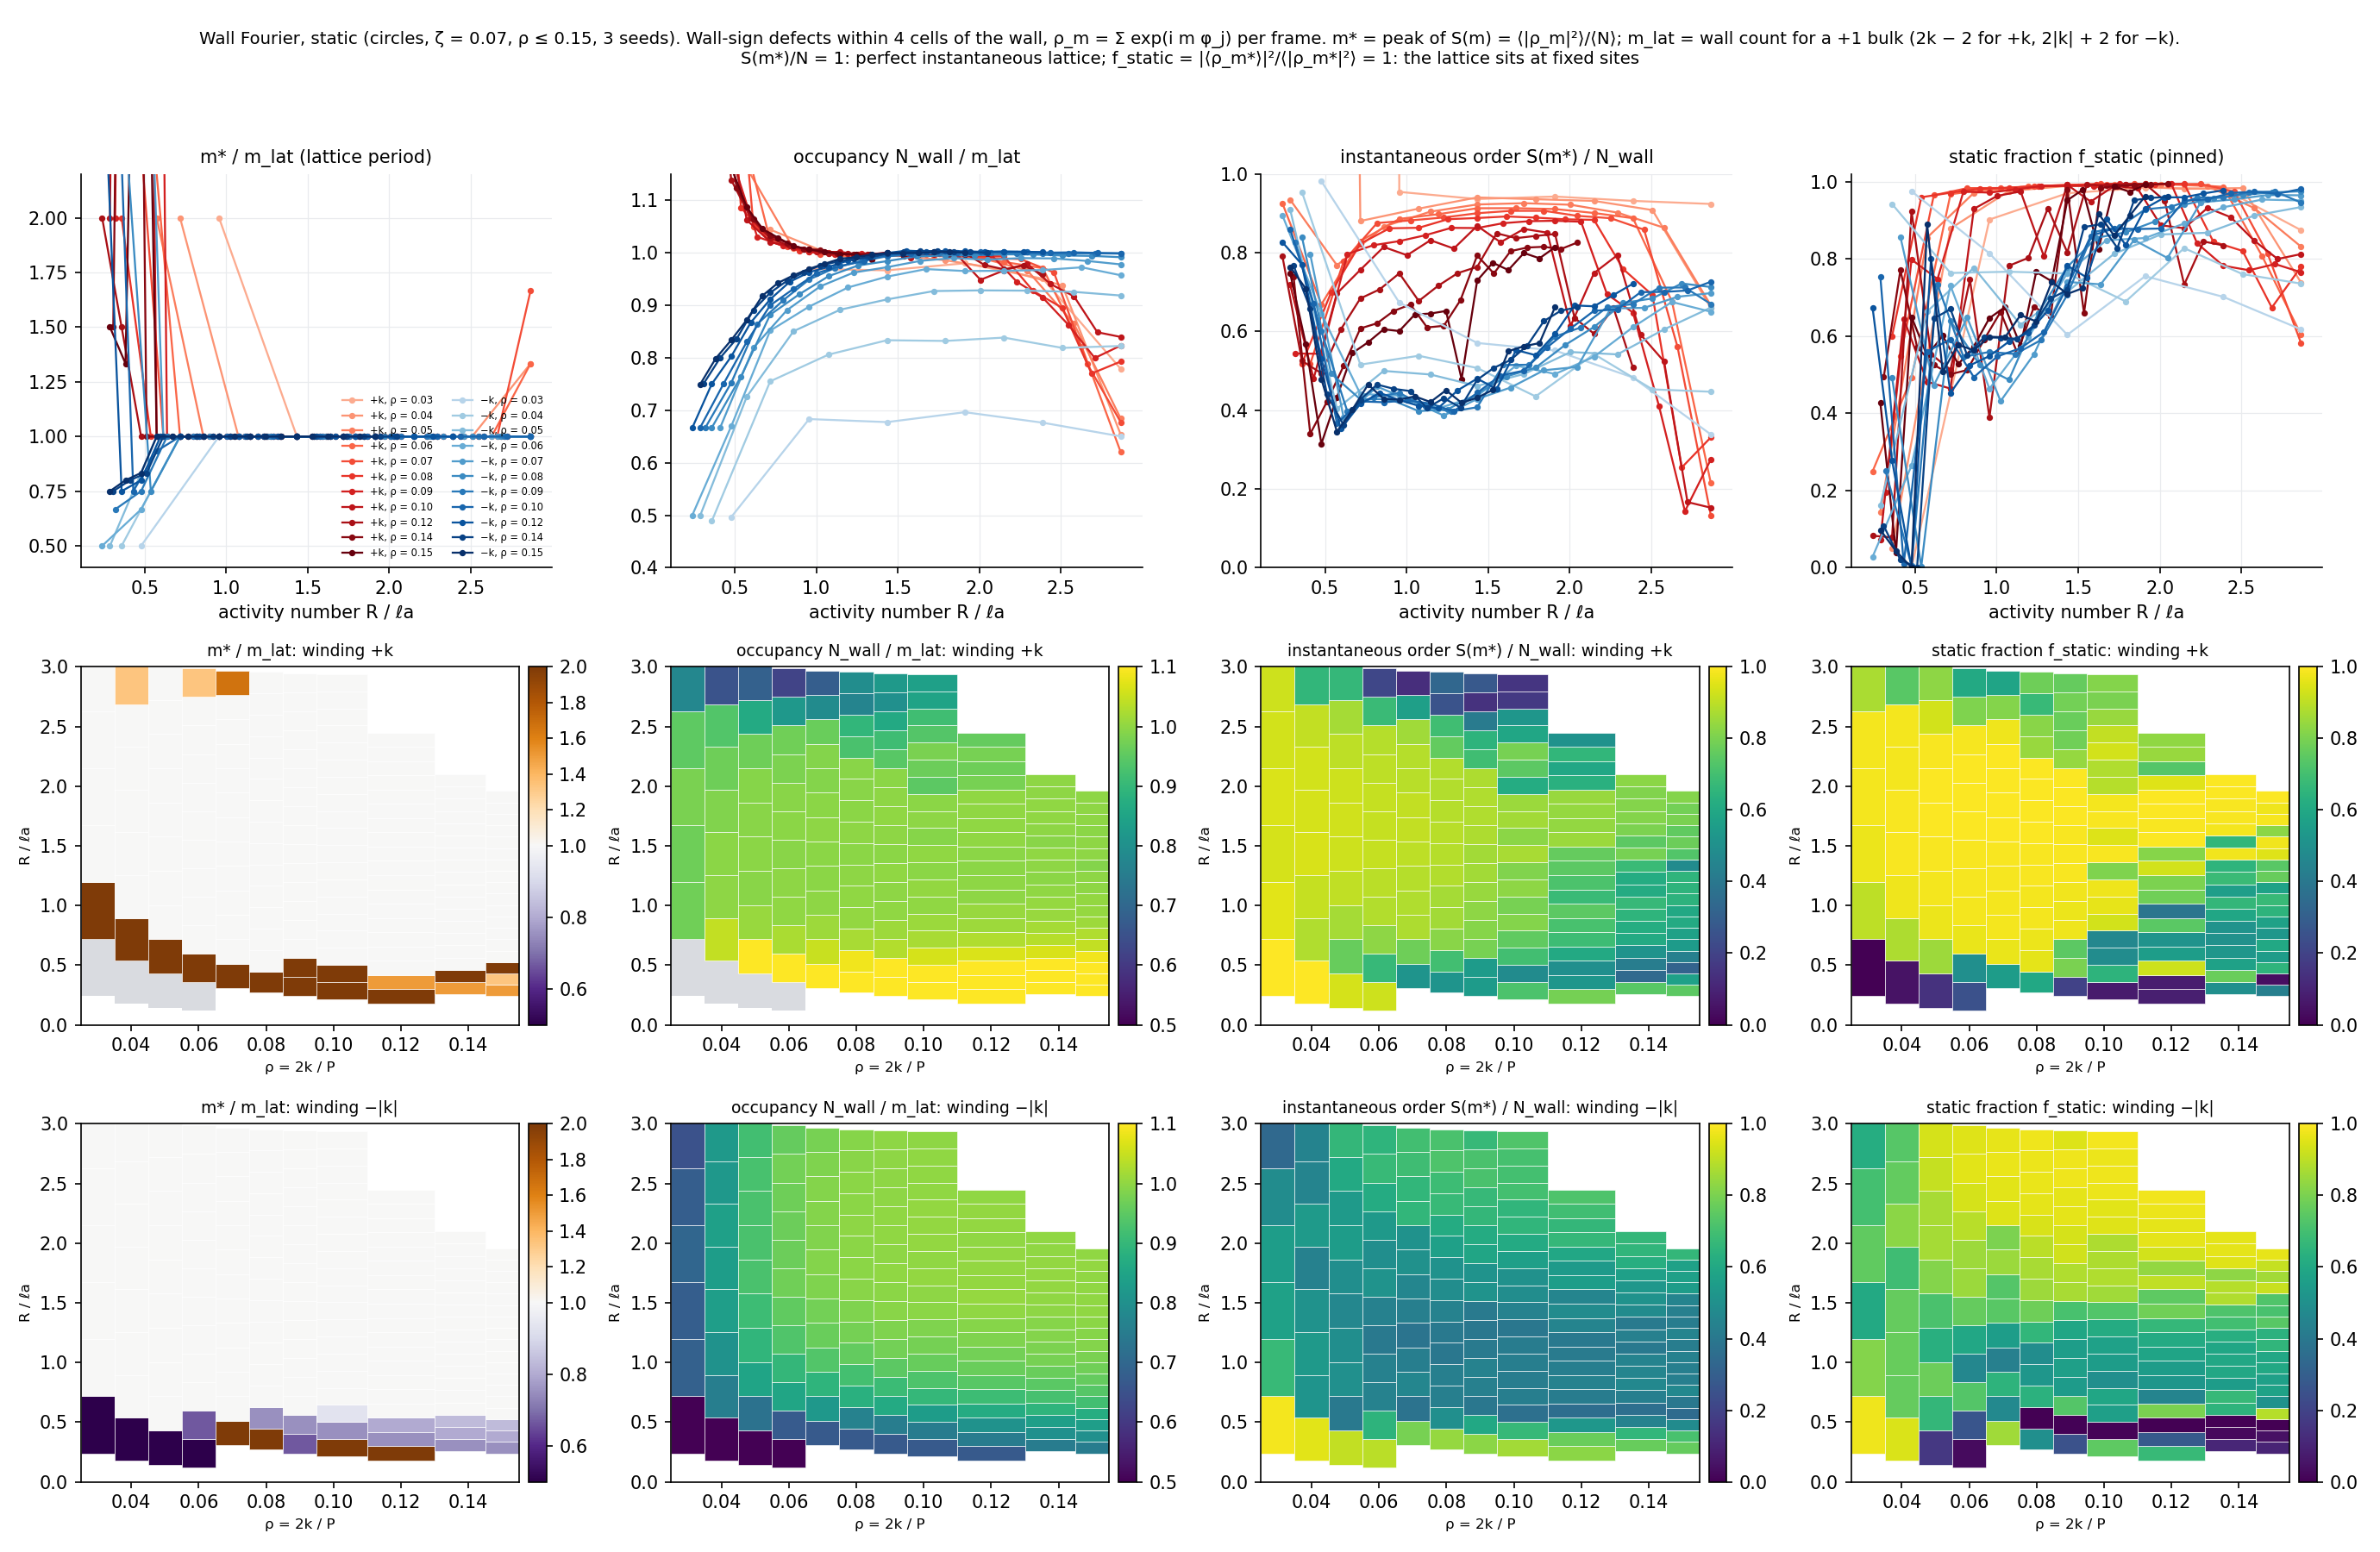
\includegraphics[width=\textwidth]{fourier_static_circles.png}
\caption{Static wall Fourier analysis of the circles. Columns: $m^*/m_\mathrm{lat}$ (with $m_\mathrm{lat}=2k-2$ for $+k$,
$2|k|+2$ for $-k$, the wall count of a $+1$ bulk), occupancy, instantaneous order, static fraction. Top: against $R/\la$,
one curve per $\rho$ (red $+k$, blue $-|k|$); middle and bottom: maps for $+k$ and $-|k|$.}\label{fig:fstat}
\end{figure}
\begin{figure}[H]\centering
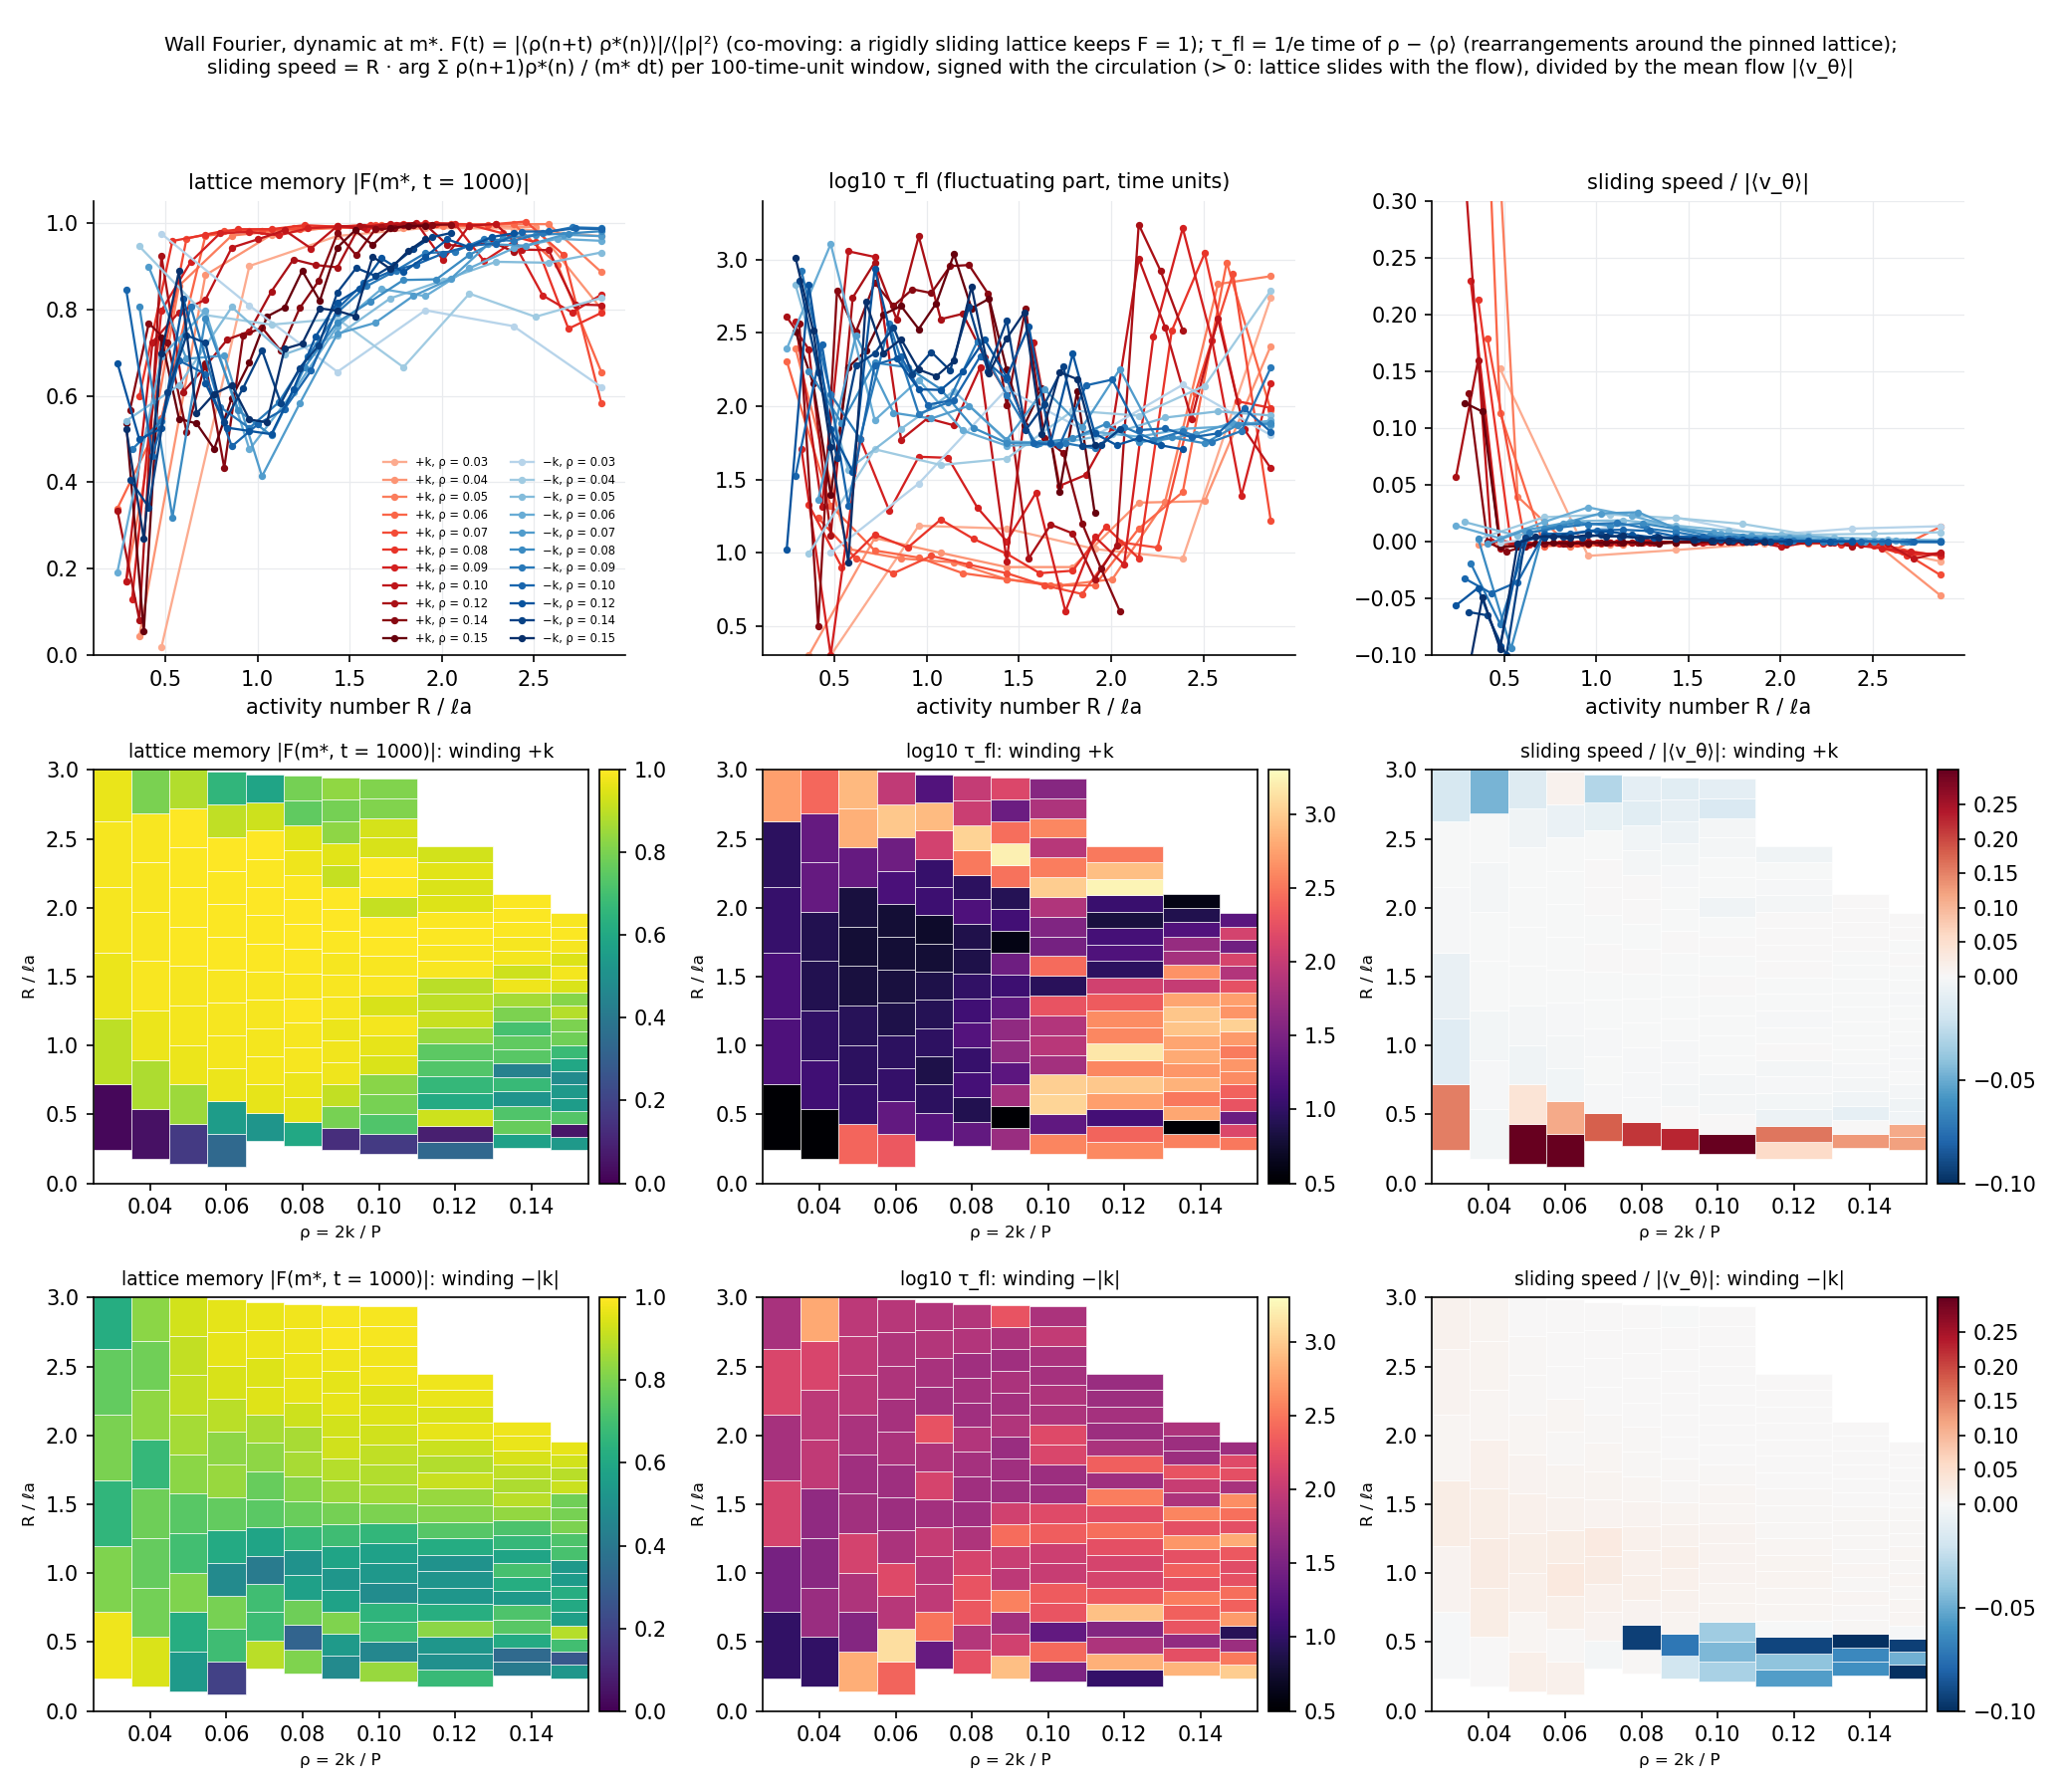
\includegraphics[width=0.9\textwidth]{fourier_dynamic_circles.png}
\caption{Dynamic wall Fourier analysis: lattice memory $|F(m^*,t=1000)|$, $\log_{10}\tau_\mathrm{fl}$ (rearrangements around the
pinned lattice) and the sliding speed divided by the mean flow $|\langle v_\theta\rangle|$ (positive: with the flow).}\label{fig:fdyn}
\end{figure}
\begin{itemize}
  \item \textbf{Period.} $m^*=m_\mathrm{lat}$ in every run with $R\gtrsim0.5$--$0.75\,\la$, for both signs: the wall lattice
        always has the period of a $+1$ bulk, $2k-2$ sites for $+k$ and $2|k|+2$ for $-k$.
  \item \textbf{Occupancy.} $+k$: 1.0 from 0.75 to $2.3\,\la$, dropping to 0.6--0.85 at $R\gtrsim2.5\,\la$ (layer loss).
        $-k$: 0.7--0.9 at low $\rho$, rising to 1 at high $\rho$ or large $|k|$ --- the vacancies that keep the mirror bulk below $+1$.
  \item \textbf{Order and pinning.} $+k$: $S/N=0.8$--0.9 at low $\rho$, 0.5--0.8 at high $\rho$; $f_\mathrm{static}\approx0.95$--1.
        $-k$: $S/N$ only 0.4--0.6, $f_\mathrm{static}$ 0.5--0.9, rising with $R$.
  \item \textbf{No sliding.} Lattice speed $<2$--3\% of $|\langle v_\theta\rangle|$ for $R>0.6\,\la$; only tiny cavities rotate.
        Lattice memory $\approx1$ for $+k$ in the layer window, 0.5--0.9 for $-k$. Rearrangement time $\tau_\mathrm{fl}\sim10$
        time units for $+k$ at low $\rho$, 100--1000 at high $\rho$, 60--100 for $-k$. \textbf{The layer is pinned, or vacant and
        melting; an ordered layer sliding with the vortex never occurs.} The earlier impression of a ``partly sliding'' layer at
        $2.87\,\la$ (static fraction 0.87) is vacancies, not sliding.
  \item \textbf{Per-defect drift} (Sec.~\ref{sec:md-drift}; $k=6$ circles analysed with the oval script): drift/$|v_w|\approx0$
        ($<1\%$) for $R=0.7$--$1.7\,\la$, $-2\%$ at $2.15\,\la$, $-18\%$ at $2.87\,\la$ (occupancy 0.78): in circles the wall defects
        move against the flow only where the lattice has vacancies (compare ovals, Sec.~\ref{sec:slattice}).
\end{itemize}

%=====================================================================
\section{Flow and tilt of the wall defects in circles}\label{sec:cflow}
Flow fields every 1000 steps (100 time units) on all seeds; methods in Secs.~\ref{sec:md-flow} and \ref{sec:md-tilt}.
\begin{figure}[H]\centering
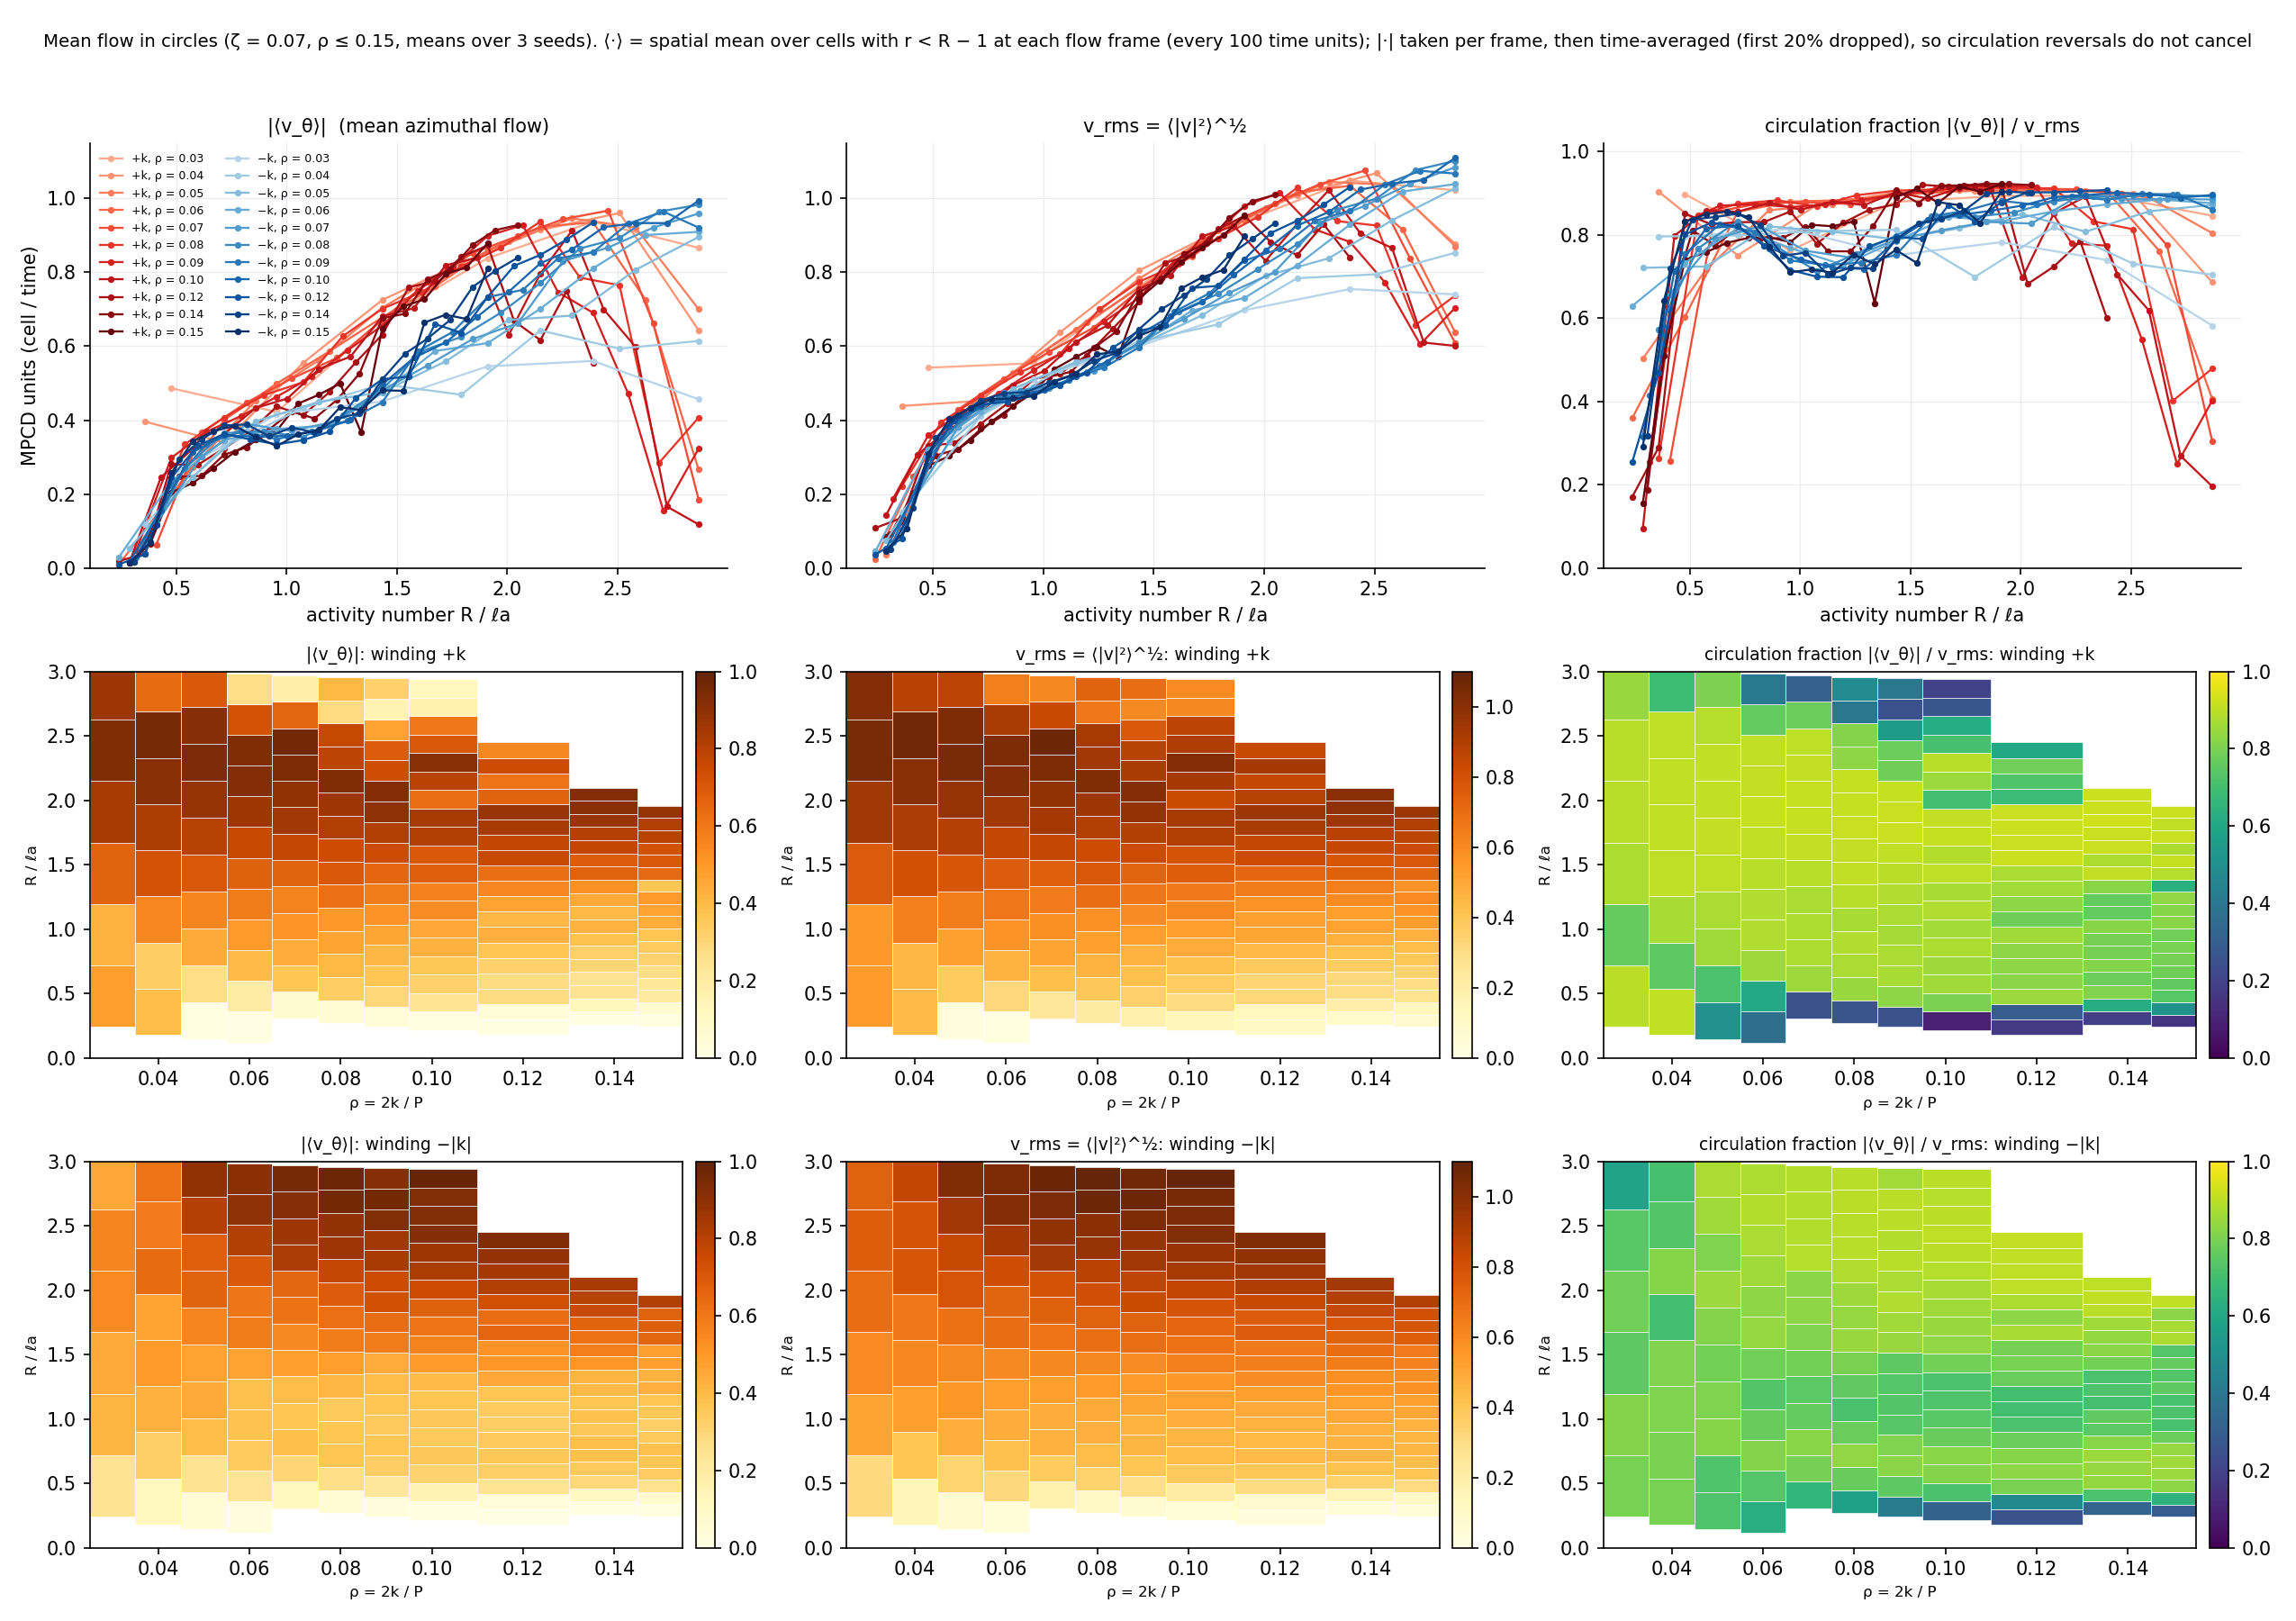
\includegraphics[width=\textwidth]{flow_mean.png}
\caption{Mean flow in circles: $|\langle v_\theta\rangle|$ (spatial mean of the azimuthal velocity per frame, absolute value,
then time-averaged), $v_\mathrm{rms}$ and the circulation fraction $|\langle v_\theta\rangle|/v_\mathrm{rms}$; curves against
$R/\la$ (red $+k$, blue $-|k|$, one per $\rho$) and maps.}\label{fig:flow}
\end{figure}
\begin{figure}[H]\centering
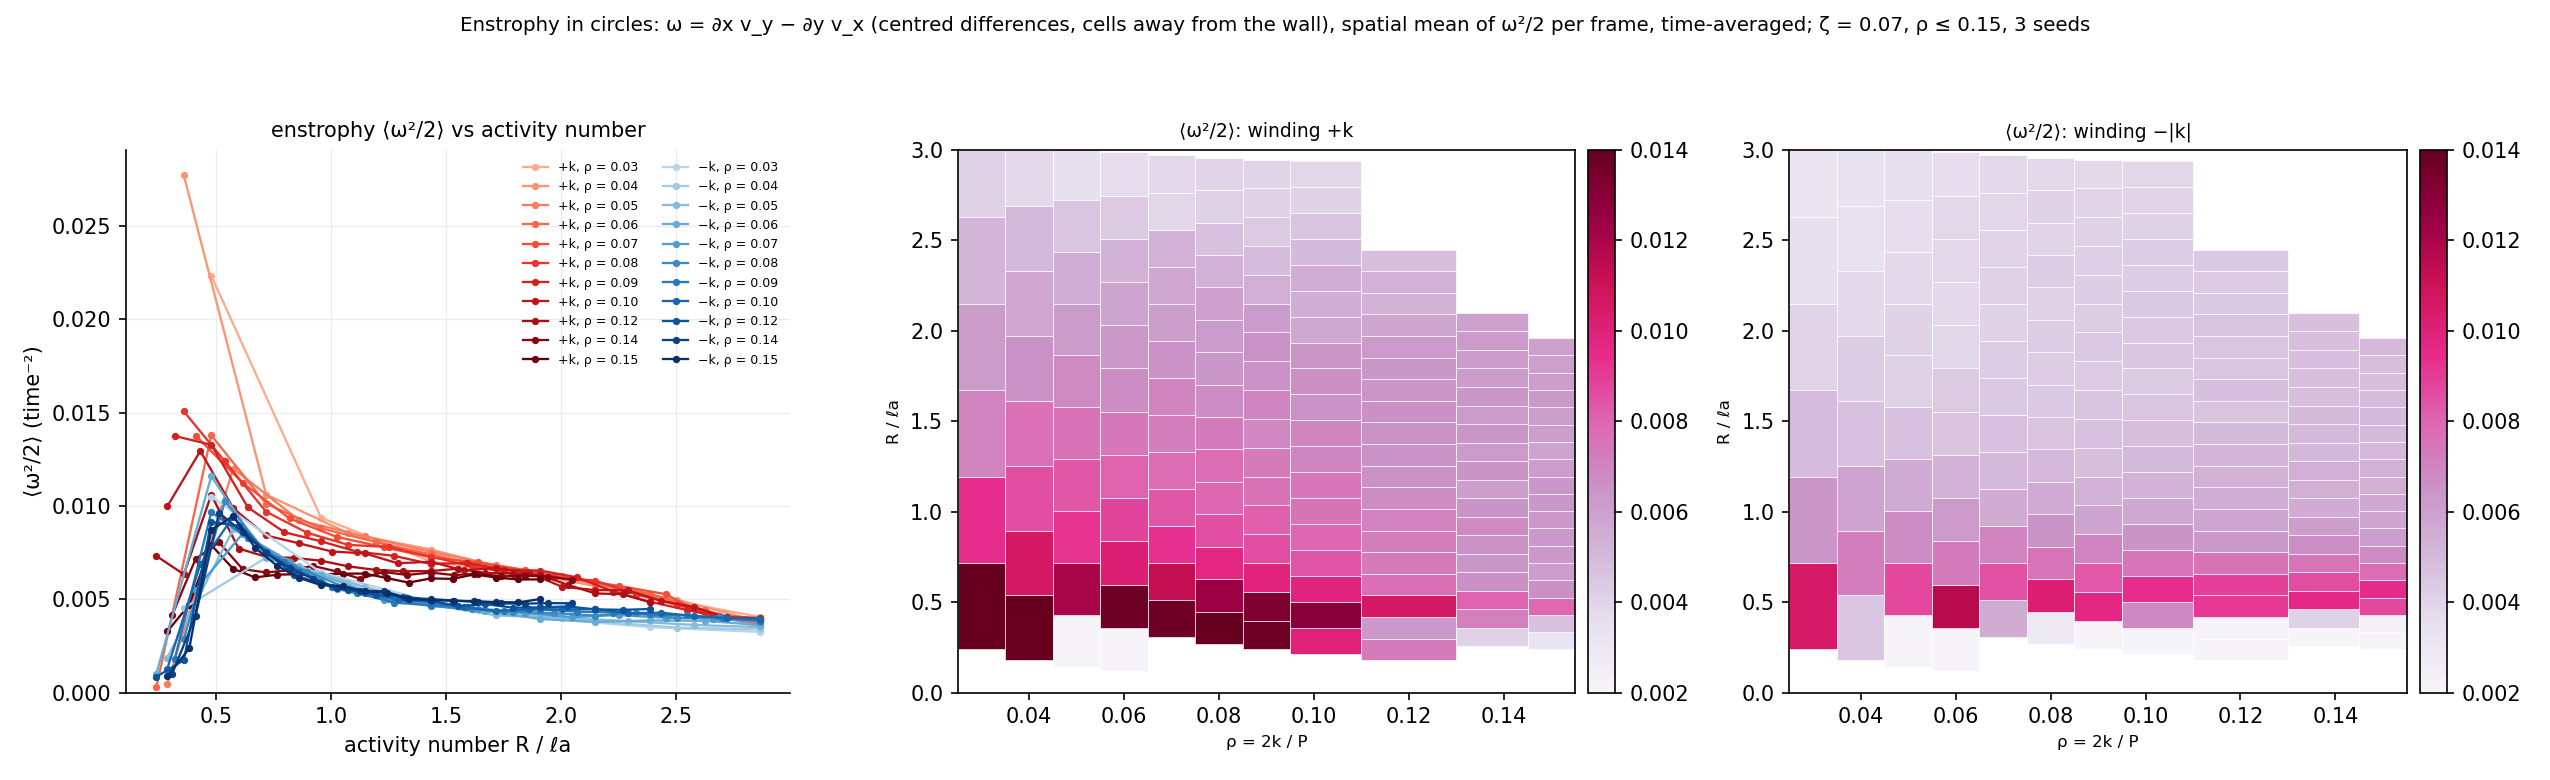
\includegraphics[width=0.9\textwidth]{flow_enstrophy.png}
\caption{Enstrophy $\langle\omega^2/2\rangle$ over interior cells.}\label{fig:enst}
\end{figure}
\begin{figure}[H]\centering
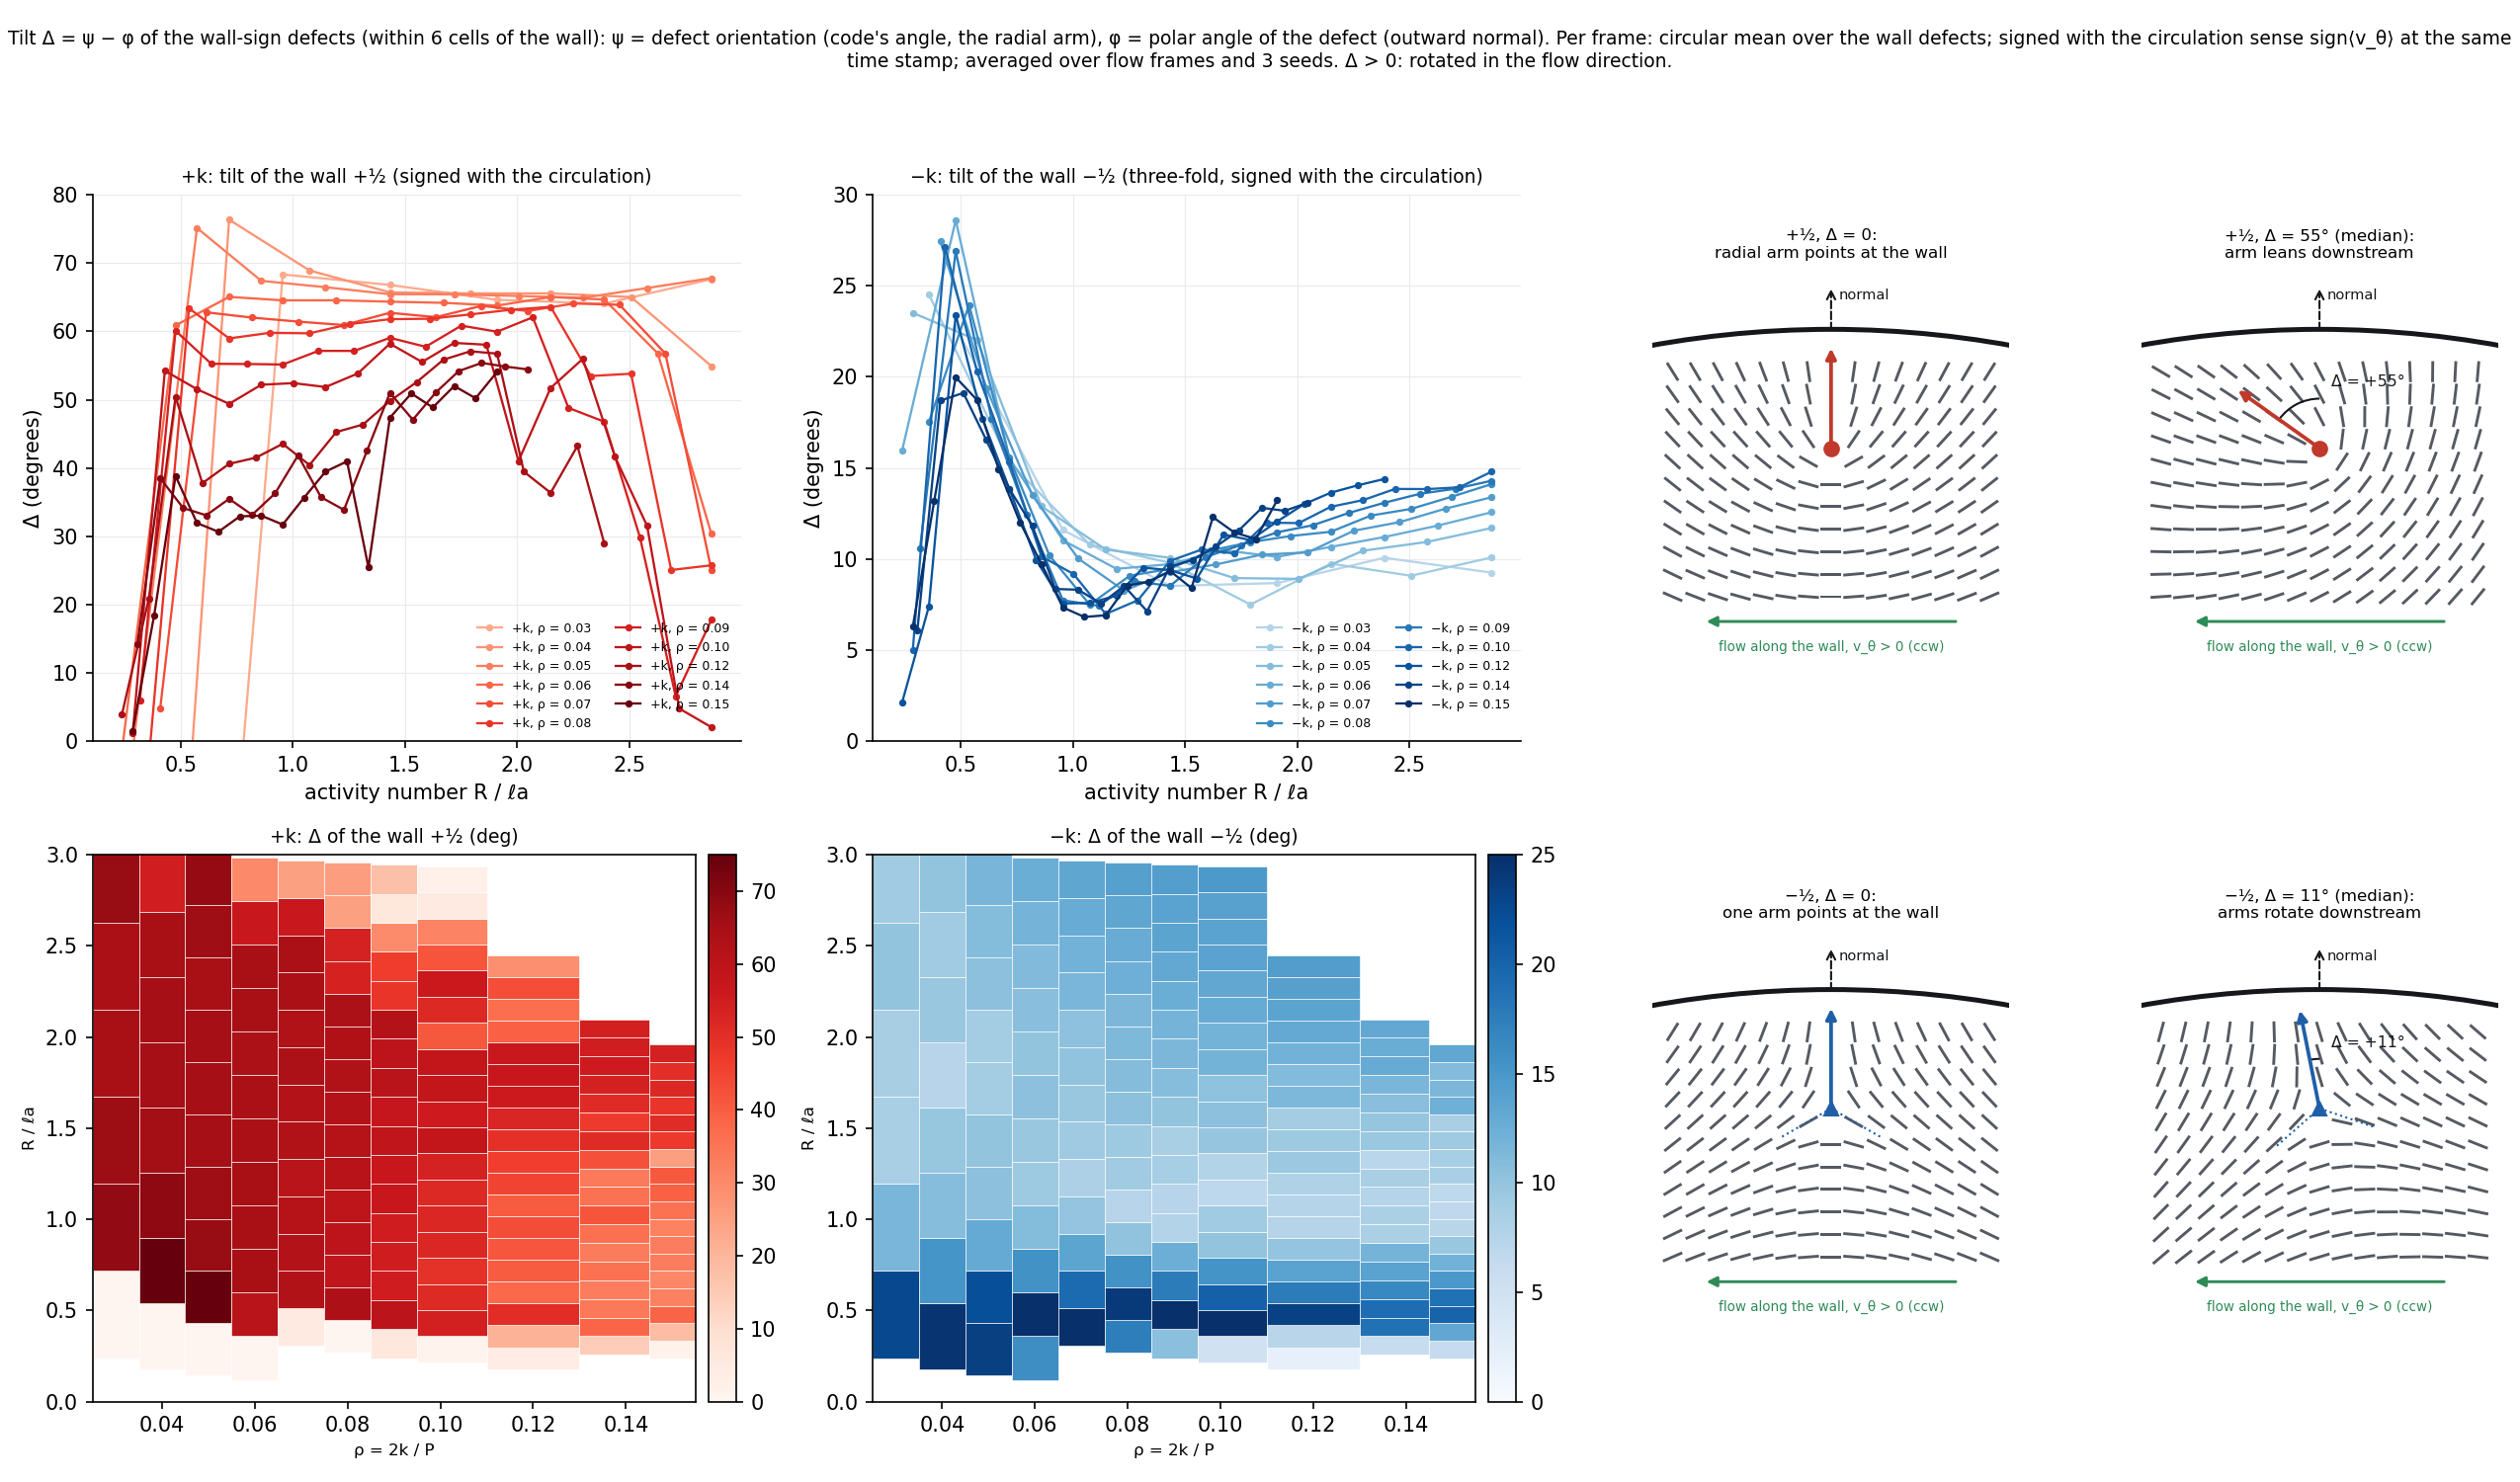
\includegraphics[width=\textwidth]{flow_tilt.png}
\caption{Tilt $\Delta=\psi-\varphi$ of the wall defects (orientation minus polar angle), signed with the circulation sense:
$+\half$ (left) and the three-fold $-\half$ (middle), with schematics (right).}\label{fig:tilt}
\end{figure}
\begin{itemize}
  \item \textbf{Circulation collapses on $R/\la$} for all $\rho$: $|\langle v_\theta\rangle|\approx0.35$ at $0.6\,\la$, 0.9--1.0
        at 2--2.5\,$\la$ (Mach $\sim1$). Circulation fraction 0.8--0.9 between 0.5 and 2.5\,$\la$; below 0.4\,$\la$ no coherent vortex
        ($k=2$: reversals, sign agreement $\approx0.5$). $+k$ circulates slightly faster than $-k$ at 1--2\,$\la$.
  \item \textbf{The vortex breaks down where the layer goes:} for $+k$ the circulation fraction falls from 0.9 to 0.2--0.4 at
        $R\gtrsim2.5\,\la$, with reversals --- the same size where the knee disappears (Table~\ref{tab:sweep}).
  \item \textbf{Enstrophy} peaks ($\approx0.01$--0.015) at 0.4--0.5\,$\la$ and decays to 0.004 at 2.9\,$\la$; $+k$ exceeds $-k$ by
        20--30\% below 2\,$\la$.
  \item \textbf{Tilt:} wall $+\half$ lean downstream by 60--65$^\circ$ at $\rho\le0.06$, decreasing to 30--40$^\circ$ at
        $\rho=0.14$--0.15 (crowded wall); the tilt vanishes where the layer is lost ($R\gtrsim2.5\,\la$) and below 0.4\,$\la$. Wall
        $-\half$ lean downstream by 8--15$^\circ$ (peak $\approx25^\circ$ at 0.5\,$\la$). The sign agrees with the circulation in
        $\approx100\%$ of frames inside the layer window.
  \item \textbf{H4} (the $+1$ bulk appears with circulation) is consistent but untested as a cause: wherever the layer exists the
        vortex exists too, and both disappear together at large $R$. The activity onset ($\zeta=0.05$, $k=9$--10) is the one case
        where the vortex fails at fixed $R/\la$ (Sec.~\ref{sec:activity}); there the bulk charge also drifts above 1.
\end{itemize}

%=====================================================================
\section{Survival of wall defects and docking in circles}\label{sec:csurv}
Two complementary measures (methods: Secs.~\ref{sec:md-labels}, \ref{sec:m-surv}). \emph{Label survival} follows the wall
defects present at a reference time, passing the label to the birth partner when a wall defect annihilates; it asks whether
the wall defects stay at the wall, whoever they are. \emph{Visit survival} follows each $+\half$ track and measures how long it
stays once it has reached the wall (Kaplan--Meier with censoring), plus the reverse process, docking of bulk $+\half$.
\begin{figure}[H]\centering
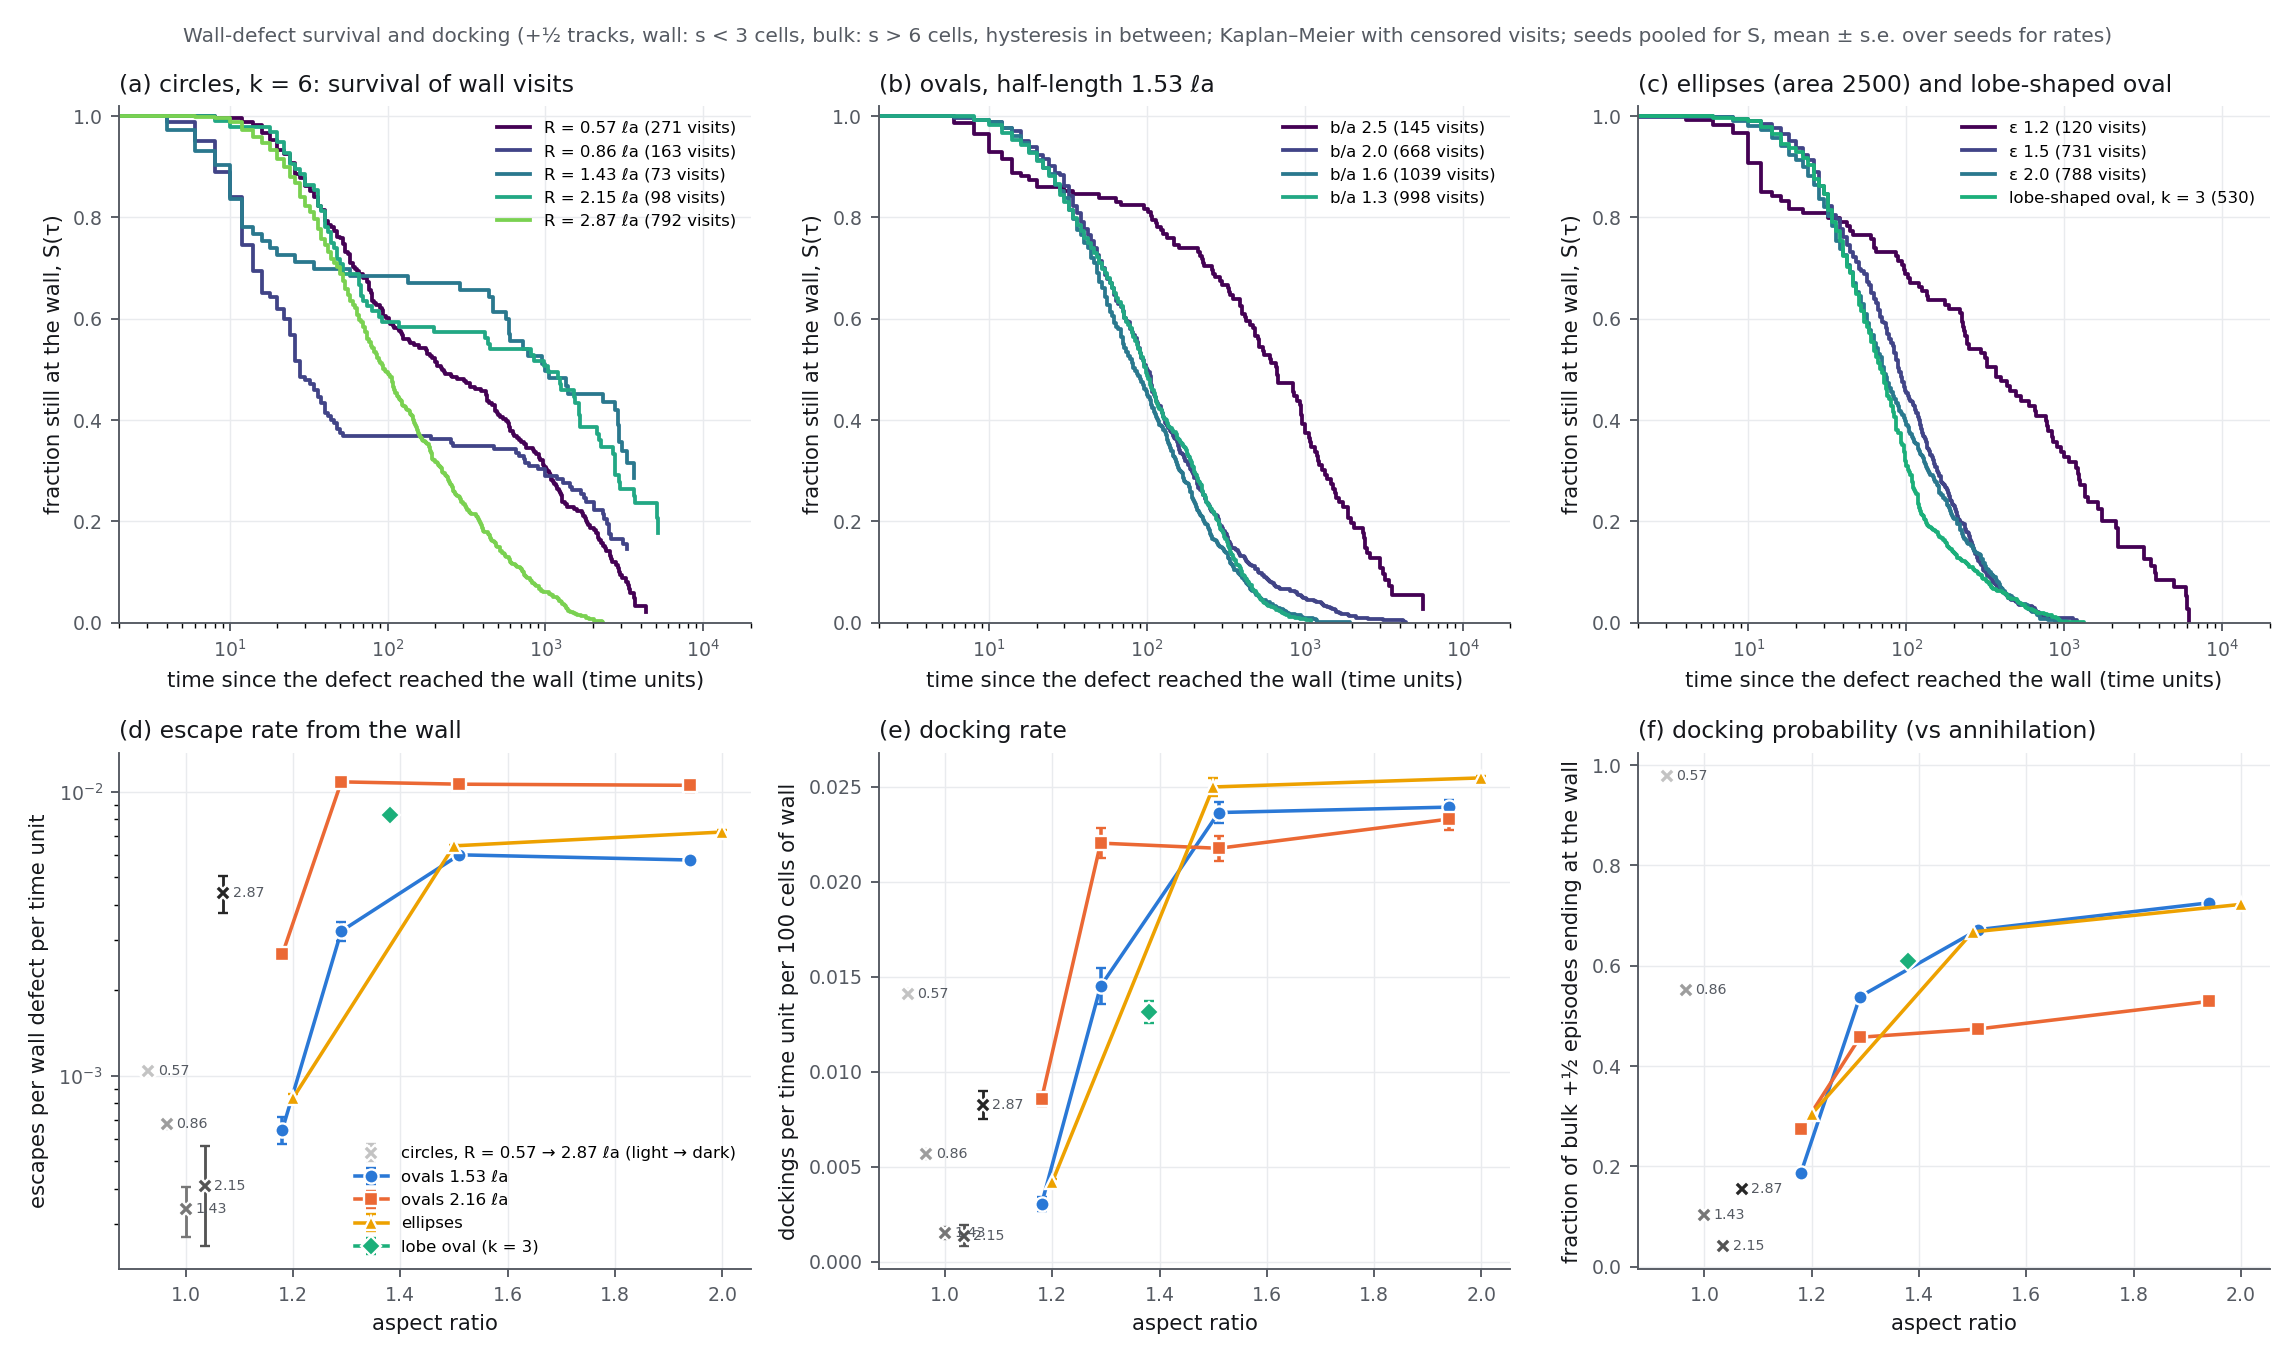
\includegraphics[width=\textwidth]{survival_docking.png}
\caption{\textbf{Survival and docking.} (a--c) Kaplan--Meier survival $S(\tau)$ of wall visits for circles ($k=6$, five sizes),
ovals of half-length $1.53\,\la$, ellipses and the lobe-shaped oval (seeds pooled; numbers of visits in the legends).
(d) Escape rate per wall defect, (e) docking rate per 100 cells of wall, (f) fraction of bulk $+\half$ episodes that end at
the wall rather than by annihilation; mean $\pm$ s.e.\ over seeds, against the aspect ratio (circles at aspect 1, light to dark
= $R=0.57\to2.87\,\la$). Wall: $s<3$ cells, bulk: $s>6$ cells.}\label{fig:surv}
\end{figure}
\begin{figure}[H]\centering
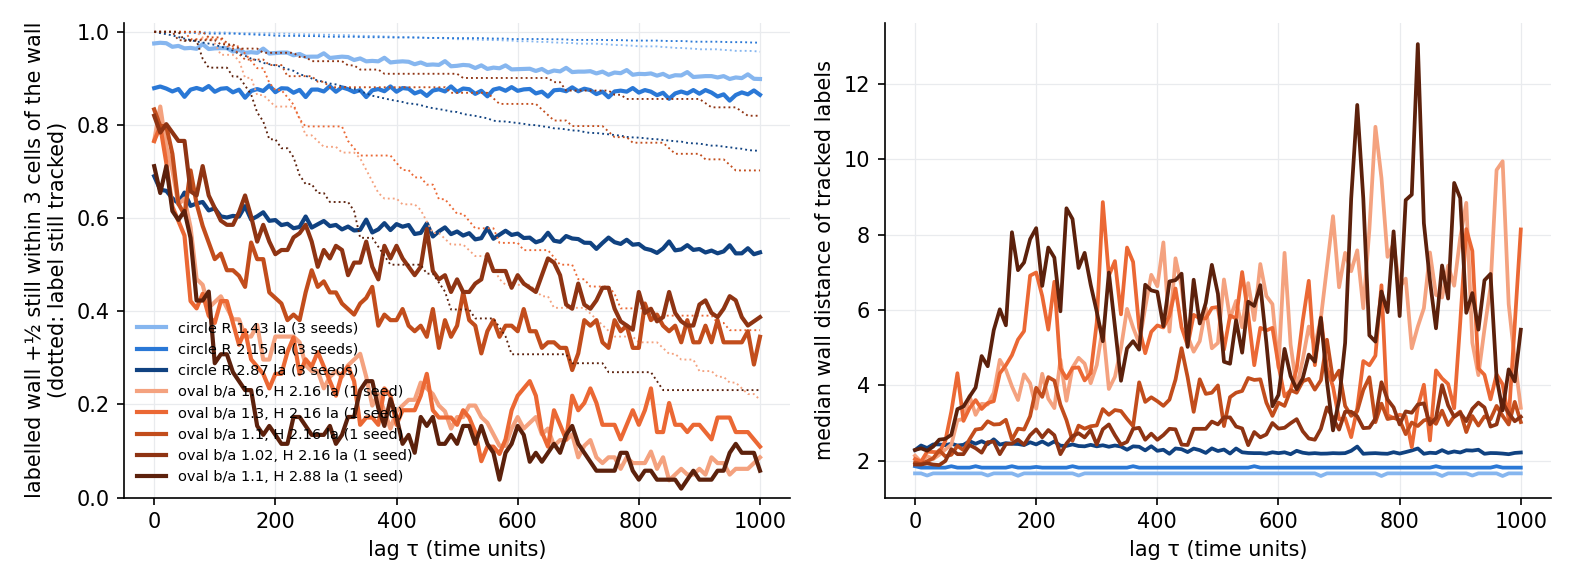
\includegraphics[width=\textwidth]{labels_circles_ovals.png}
\caption{Label survival: fraction of the labelled wall defects within 3 cells of the wall (left) and median wall distance of
tracked labels (right) against the time since labelling, circles ($k=6$, 3 seeds per size) and ovals (half-length 2.16 and
$2.88\,\la$, 1 seed).}\label{fig:labels}
\end{figure}
\begin{table}[H]\centering\small
\caption{Circles, $k=6$, 3 seeds: wall-visit survival and docking (\texttt{reports/master/data/survival\_docking.txt}).
Visits: wall visits with observed start; $t_{1/2}$: time at which $S=\half$ (time units); docking rate per 100 cells of wall per time unit; bulk time: median time in the bulk before docking.}\label{tab:csurv}
\begin{adjustbox}{max width=\textwidth}
\begin{tabular}{lcccccccc}\toprule
$R/\la$ & visits & wall $+\half$ & escape rate ($10^{-3}$) & $S(1000)$ & $t_{1/2}$ & docking rate & $P_\mathrm{dock}$ & bulk time\\\midrule
0.57 & 271 & 10.9 & $1.04\pm0.02$ & 0.31 & 220 & 0.014 & 0.98 & 72\\
0.86 & 163 & 10.1 & $0.67\pm0.02$ & 0.29 & 28 & 0.006 & 0.55 & 76\\
1.43 & 73 & 10.0 & $0.34\pm0.07$ & 0.50 & 1000 & 0.0015 & 0.10 & 25\\
2.15 & 98 & 9.9 & $0.41\pm0.16$ & 0.51 & 1044 & 0.0014 & 0.04 & 21\\
2.87 & 792 & 8.4 & $4.4\pm0.7$ & 0.06 & 96 & 0.008 & 0.15 & 24\\\bottomrule
\end{tabular}
\end{adjustbox}
\end{table}
\begin{itemize}
  \item \textbf{In clean circles the wall defects stay.} At 1.43 and $2.15\,\la$ half of the wall visits last longer than 1000
        time units, and a wall defect escapes about once per 3000 time units (escape rate $3$--$4\times10^{-4}$). Label survival:
        84--94\% of the labelled wall defects are still at the wall after 1000 time units; the median wall distance of tracked labels
        stays at 1.7--2.3 cells. The few visits in these runs (73--98) are because the layer barely exchanges.
  \item \textbf{Docking is rare:} only 4--10\% of bulk $+\half$ excursions end at the wall; the rest end by annihilating with a
        $-\half$ in the bulk. The $2k-2$ layer and the bulk are almost decoupled populations.
  \item \textbf{Large circle ($2.87\,\la$):} escape rate 13$\times$ higher, $S(1000)=0.06$; labels 41--59\% at the wall after 1000.
        This is the degraded layer of Sec.~\ref{sec:sweep}: vacancies (occupancy 0.78), upstream drift (Sec.~\ref{sec:clattice}) and
        exchange.
  \item \textbf{Small circles} ($\le0.86\,\la$) are a different regime: no or few bulk pairs (0 and 0.4 $-\half$ per frame), and
        the cavity is only a few wall-to-bulk thresholds across, so $+\half$ cross the 3/6-cell thresholds often, visits are short and
        docking is frequent ($P_\mathrm{dock}=0.55$--0.98). The wall lattice is weakly pinned at $0.57\,\la$ (static fraction 0.51)
        and mostly pinned at $0.86\,\la$ (0.83).
  \item The layer empties, when it does, by undocking: at most 10\% of wall visits end in annihilation (exchange analysis).
\end{itemize}
\open{The docking pathway itself (H7: do bulk $+\half$ circulate along the layer edge and insert into the largest gaps?) has not
been analysed yet; the tracks needed for it exist.}

%=====================================================================
\section{Activity: does it enter only through $\la$?}\label{sec:activity}
H3: if activity entered only through $\la$, cavities with the same $R/\la$ would behave identically at any $\zeta$. Test at
$R=1.434\,\la$ (radius rescaled with the measured $\la(\zeta)$: $R=37.5$, 34.9, 31.8, 29.6, 27.3 for $\zeta=0.05$, 0.06, 0.07,
0.09, 0.11), $k=2\dots10$, 3 seeds. A bulk-sized patch of periodic box holds the same $\pi R^2/\la^2\approx6.5$ defects at
every activity.
\begin{table}[H]\centering\small
\caption{Activity scan at fixed $R/\la=1.43$ (site rule; ranges over $k=2\dots10$). Gap: $+\half$ density at $s\approx3$--4.5
relative to the bulk. Slope: $\mathrm{d}Q/\mathrm{d}s$ between $s=3$ and 5 ($k=8$), the flatness of the $+1$ plateau.}\label{tab:act}
\begin{tabularx}{\textwidth}{lccccccX}\toprule
$\zeta$ & $q_b$ & $P(q_b=+1)$ & pairs/frame & $\Phi$ & gap & slope & behaviour\\\midrule
0.05 & 1.16--1.81 & 0.36--0.68 & 0.6--1.3 & 0.83--0.92 ($k\le8$) & -- & -- & onset: vacant sites (e.g.\ $k=6$: 9.0 of 10), vortex fails at $k=9,10$\\
0.06 & 1.05--1.15 & 0.67--0.83 & 1.3--1.7 & 0.85--0.95 & shallow & 0.13 & mild onset\\
\textbf{0.07} & \textbf{1.01--1.09} & \textbf{0.89--0.96} & 1.5--2.0 & 0.89--0.97 & $\sim5\times$ & \textbf{0.07} & clean\\
0.09 & 1.01--1.05 & 0.77--0.92 & 1.9--2.4 & 0.88--0.99 & $\sim4\times$ & 0.15 & clean bulk; centre depleted\\
0.11 & 1.0--1.2 ($k\le6$) & 0.6--0.8 & 2.3 & 0.98 & $\sim1.5\times$ & 0.32 & gap closes; split ill-defined for $k\ge7$\\\bottomrule
\end{tabularx}
\end{table}
\begin{itemize}
  \item \textbf{$\zeta=0.05$ is the turbulence onset}: few dynamical defects (no pair in 22--50\% of frames against $\approx5\%$ at
        0.07), sites often vacant, bulk charge rising with $k$ up to 1.8, and at $k=9$, 10 the vortex keeps reversing
        ($\Phi_\mathrm{persist}=0.37\pm0.21$, $0.51\pm0.10$). Periodic boxes agree: the defect number drops sharply below
        $\zeta\approx0.06$ and fluctuations decorrelate three times more slowly.
  \item \textbf{$\zeta=0.11$: the layer--bulk gap closes.} The wall peak is at the same $s\approx1.2$ cells at every activity, but the
        gap at $s\approx3$--4.5 is $5\times$ below the bulk at 0.07 and only $1.5\times$ at 0.11. The layer has a fixed width in
        cells while the bulk density grows as $1/\la^2$, so at high activity bulk defects press against the layer.
  \item \textbf{$\zeta=0.09$} gives a clean bulk charge, but the vortex empties the centre (Table~\ref{tab:dens}).
  \item In $r/R$, bulk $g_{++}$ collapses for $\zeta=0.05$--0.09; $g_{--}$ only up to $\approx0.5R$ at 0.05 (Fig.~\ref{fig:gact}).
  \item \textbf{Conclusion:} activity does not enter only through $\la$. The working activity $\zeta=0.07$ balances onset effects
        (below) and compressibility (above).
\end{itemize}
\begin{figure}[H]\centering
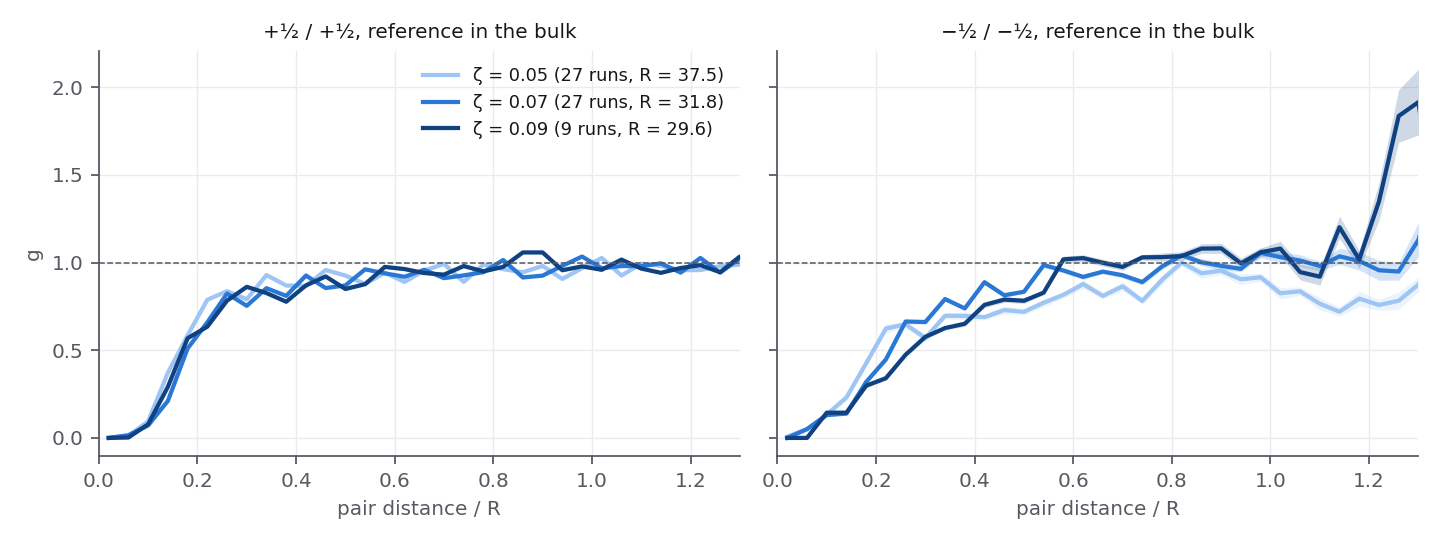
\includegraphics[width=0.85\textwidth]{g_act.png}
\caption{Bulk pair correlations at $\zeta=0.05$, 0.07, 0.09 in units of $r/R$ ($R=1.43\,\la$ at each activity).}\label{fig:gact}
\end{figure}
\paragraph{Density stratification.} \SIcand The vortex centrifuges particles towards the wall (compressibility, Mach number
$\sim1$). In cavities with $k=8$ at the activity-scan radii:
\begin{table}[H]\centering\small
\caption{Particle occupancy per cell ($\langle n\rangle=20$; Poisson standard deviation 4.47), by distance $s$ from the wall.}\label{tab:dens}
\begin{adjustbox}{max width=\textwidth}
\begin{tabular}{lcccccc}\toprule
$\zeta$ & SD / Poisson & $s<5$ & centre $s>20$ & $P(n<10)$ all & $P(n<10)$ centre & $-\half$ cores\\\midrule
0.07 & 1.5 & 25 & 14 & 4.5\% & 15\% & 15\\
0.09 & 2.0 & 28 & 9 & 15\% & 60\% & 11\\
0.11 & 2.2 & 29 & 8 & 17\% & 70\% & 11\\\bottomrule
\end{tabular}
\end{adjustbox}
\end{table}
The gap region ($s=3$--5) is over-dense (25--28), so low occupancy does not explain the closing gap. Even at $\zeta=0.07$ the
centre is depleted by $\approx30\%$; $-\half$ cores sit in depleted cells. collOp 21 is a density-modulated dipole, so the active
stress varies with this stratification. This is a property of particle-based active nematics at finite Mach number and should
be stated in the methods; a low-Mach control (higher $k_BT$) would change the whole calibration and is not planned.


\part{Ellipses and Cassini ovals}
%=====================================================================
\section{Shapes, sizes and run sets}\label{sec:ssetup}
\paragraph{Why these shapes.} Every cavity here is simply connected with one wall, so the imposed winding $k$ fixes the same
total charge as in a circle. Changing the shape at fixed $k$ (and fixed $\rho$) separates topology from geometry (H1).
\begin{itemize}
  \item \textbf{Cassini ovals} $d_1d_2=b^2$ with foci at $(\pm a,0)$ (Sec.~\ref{sec:md-cassini}): a one-parameter family from the
        circle ($a=0$) through convex ovals ($b/a\ge\sqrt2$) to a concave neck ($1<b/a<\sqrt2$) and the lemniscate ($b=a$).
        Half-length $\sqrt{a^2+b^2}$, half-height $b^2/(2a)$ for $b/a<\sqrt2$, waist $2\sqrt{b^2-a^2}$. Aspect ratio = length/height.
        Winding imposed uniformly in arclength (eMode 3). Families are labelled by their half-length (H34, H48, H64 cells $=1.53$,
        2.16, $2.88\,\la$) and $b/a$.
  \item \textbf{Ellipses} with semi-axes $A=\varepsilon B$ (along $x$) and $B$, area 2500 ($\sqrt{A/\pi}=1.27\,\la$), arclength-uniform
        winding (eMode 2); $\varepsilon=1.2$, 1.5, 2.0. A second convex family with a different curvature profile (no flattened sides).
\end{itemize}

\begin{table}[H]\centering\small
\caption{Oval and ellipse run sets ($\zeta=0.07$ unless passive). Steps: warm-up + production. All in \texttt{runs/cassini/}.}\label{tab:ssets}
\begin{tabularx}{\textwidth}{llXcl}\toprule
set & cavities & shapes / parameters & seeds & steps\\\midrule
T1, T2 & validation & passive $k=3$: $a=0$, $b/a=1.6$, 1.2; eMode 0 and 3 & 1 & short\\
P1 & H48, H64 & $b/a=1.6$, 1.3, 1.1; $k=6$ & 1 & 10k + 40k\\
P2 & H48, H64 pinched & $b/a=1.01$--1.05, $k=6$; passive $b/a=1.02$, 1.01 & 1 & 10k + 40k\\
P3 & H34 small ovals & $b/a=2.5$, 2.0, 1.6, 1.3, $k=6$ & 3 & 10k + 100k\\
P3 & H48 pinched, high $k$ & $b/a=1.02$, $k=12$, 15, 18, 20; passive $k=18$, 20 & 1 & 10k + 100k\\
P4 & lobe-shaped oval & H30.4, $b/a=1.8$ (area and aspect of one lobe of H64 $b/a=1.01$), $k=3$ & 3 & 10k + 100k\\
P5 & passive references & H34 $b/a=2.5$--1.3 and the three ellipses, $k=6$ (5 Oct) & 1 & 10k + 30k\\
W1 & H48 size series & $b/a=2.5$, 2.0, 1.6, 1.3, $k=6$ & 3 & 10k + 100k\\
W2 & H34 $k$ scan & $b/a=2.0$, 1.6; $k=2$, 4, 8, 10, 12 ($k=6$ = P3) & 3 & 10k + 100k\\
W3 & ellipses & $\varepsilon=1.2$, 1.5, 2.0, $k=6$, eMode 2 & 2 & 10k + 100k\\
W4 & H64 seeds & $b/a=1.3$, 1.1: seeds 2, 3 (seed 1 = P1) & 2 & 10k + 40k\\\bottomrule
\end{tabularx}
\end{table}

\paragraph{Matching ovals with circles.} An oval has no single radius, so the comparison is made in every size measure at once,
at matched linear defect density $\rho=2k/P$ (Table~\ref{tab:match}). The test is whether an oval lies inside the region where
circles keep the layer (0.75--$2\,\la$, Sec.~\ref{sec:sweep}) in all of them.
\begin{table}[H]\centering\small
\caption{Ovals and circles: density and candidate size measures (units of $\la$).}\label{tab:match}
\begin{adjustbox}{max width=\textwidth}
\begin{tabular}{lccccccc}\toprule
cavity & $k$ & aspect & $\rho=2k/P$ & $\sqrt{A/\pi}$ & half-length & inscribed $r$ & $2A/P$\\\midrule
circle $R=1.43\,\la$ & 6 & 1 & 0.060 & 1.43 & 1.43 & 1.43 & 1.43\\
circle $R=1.07\,\la$ & 3 & 1 & 0.040 & 1.07 & 1.07 & 1.07 & 1.07\\
oval H34 $b/a=2.5$ & 6 & 1.17 & 0.060 & 1.42 & 1.53 & 1.30 & 1.41\\
oval H34 $b/a=1.6$ & 6 & 1.51 & 0.066 & 1.27 & 1.53 & 1.01 & 1.23\\
oval H34 $b/a=1.3$ & 6 & 1.94 & 0.069 & 1.15 & 1.53 & 0.79 & 1.07\\
oval H48 $b/a=1.6$ & 6 & 1.51 & 0.046 & 1.80 & 2.16 & 1.43 & 1.74\\
lobe-shaped oval & 3 & 1.38 & 0.036 & 1.18 & 1.37 & 1.00 & 1.16\\\bottomrule
\end{tabular}
\end{adjustbox}
\end{table}
The smallest measure, the inscribed radius, is 0.79--1.01\,$\la$ for the small ovals that lose the layer; circles of 0.72 and
0.96\,$\la$ at the same density keep a clean layer (Sec.~\ref{sec:sweep}). Every elongated oval therefore sits inside the circles'
layer region in every size measure.

%=====================================================================
\section{Passive ovals and ellipses}\label{sec:spassive}
Passive references of the shapes used in the active comparison (P5, $k=6$: the four small ovals and the three ellipses), the
pinched ovals (P2, P3) and the validation shapes (T2). Galleries: top rows of Figs.~\ref{fig:maps-small} and \ref{fig:maps-ell},
and the last two panels of Fig.~\ref{fig:maps-large}; profiles dashed in Figs.~\ref{fig:prof-small} and \ref{fig:prof-ell}.
\begin{itemize}
  \item \textbf{All $2k$ imposed defects sit at the wall on fixed sites, bulk charge 0}, for every shape, as in circles. The
        arclength anchoring (eMode 2 and 3) spaces them evenly along the wall, including the flat sides of the ovals and the
        tips of the ellipses.
  \item \textbf{Pinched ovals} ($b/a=1.02$, waist 13.5 cells, $k=6$): all 12 $+\half$ present; the two imposed defects closest to the
        neck sit inside the neck rather than on its wall (Fig.~\ref{fig:maps-large}). At $k=18$ (imposed density 0.15) all 36 sit in
        a tight wall lattice.
  \item Imposed-defect depth follows the spacing as in circles (the shapes here have $\rho=0.05$--0.07, depth $\approx2$ cells).
\end{itemize}
\begin{figure}[H]\centering
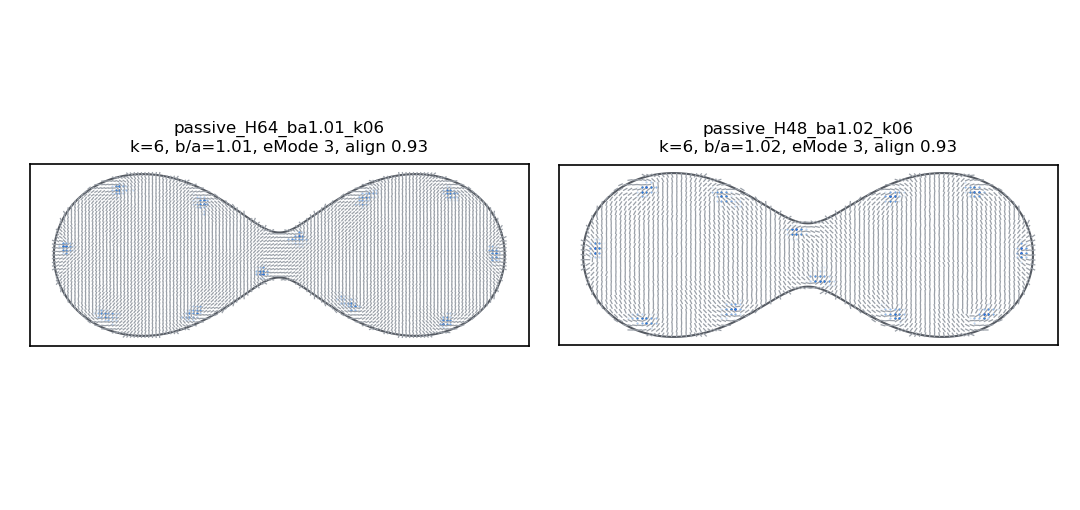
\includegraphics[width=\textwidth]{cassini_passive_pinched.png}
\caption{Passive pinched ovals ($b/a=1.02$ and 1.01, $k=6$): all imposed defects present and at the wall or in the neck.}\label{fig:passpinch}
\end{figure}

%=====================================================================
\section{Active ovals and ellipses: where the defects sit}\label{sec:sdist}
Same treatment as for circles (Sec.~\ref{sec:cdist}): time-averaged maps on a common scale and profiles against the exact distance
from the wall (Sec.~\ref{sec:m-dist}). Seed 1 of each cavity.
\begin{figure}[H]\centering
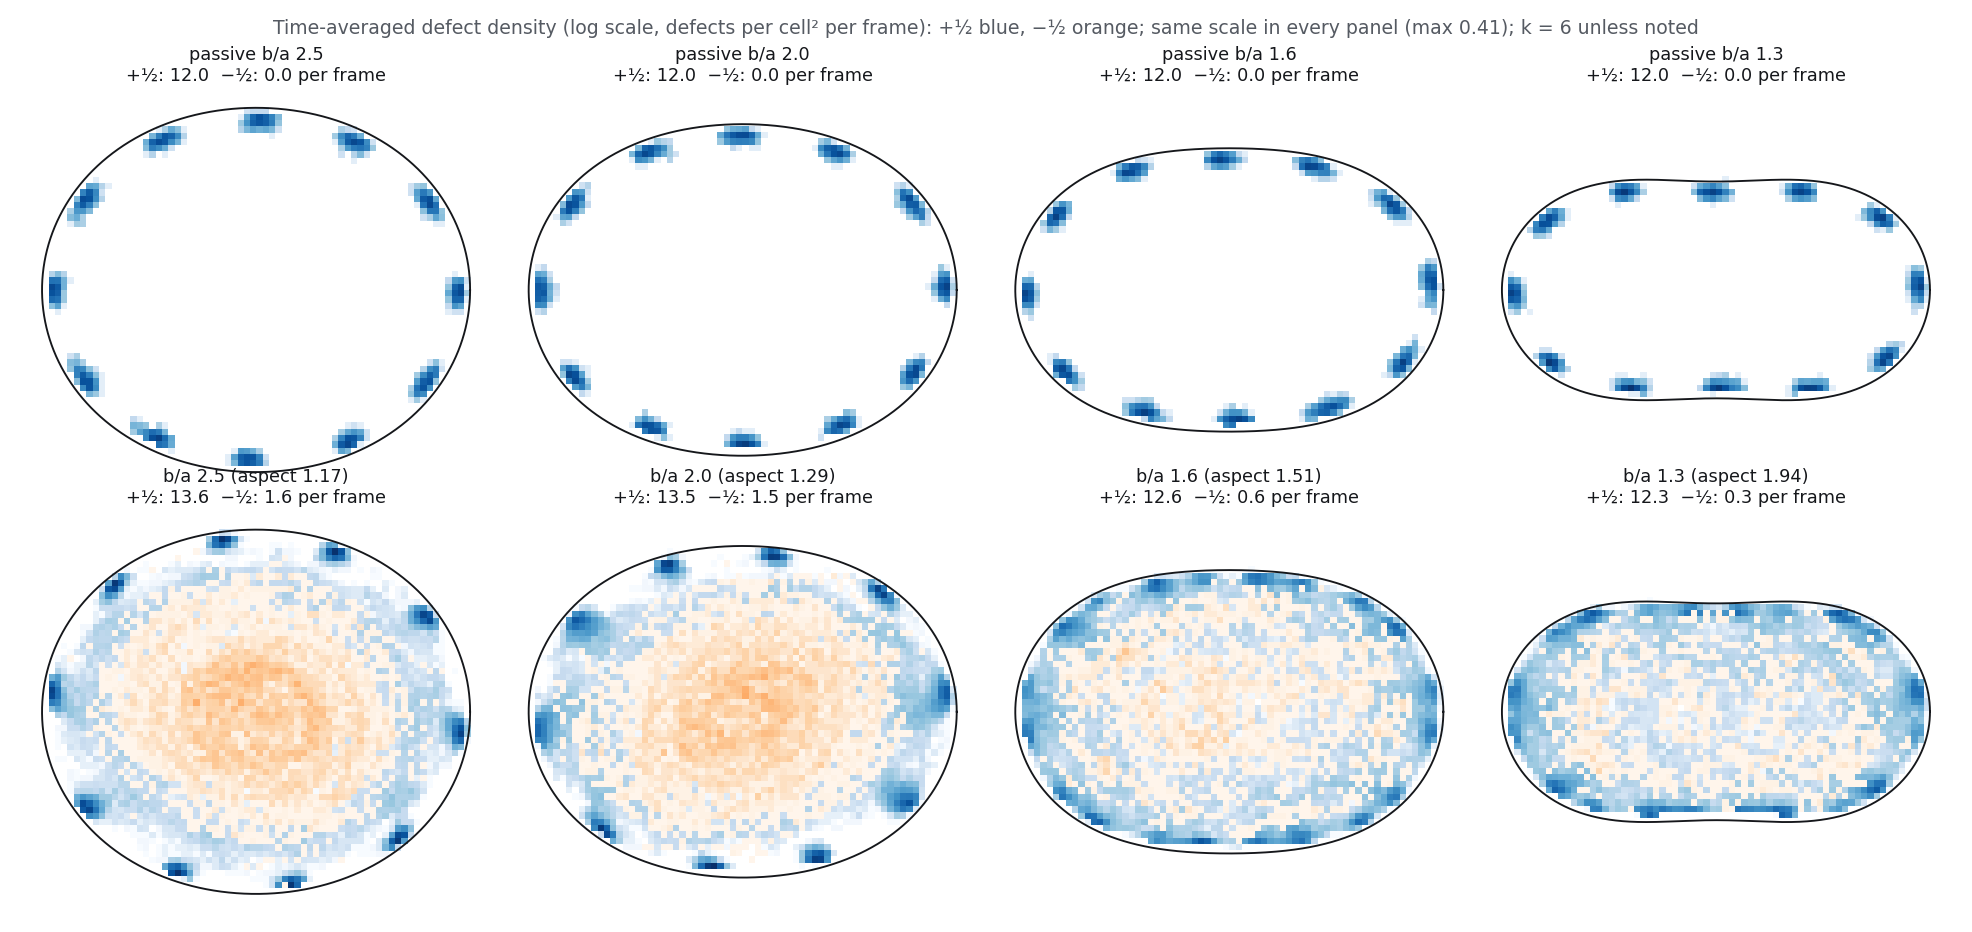
\includegraphics[width=\textwidth]{maps_ovals_small.png}
\caption{Small ovals (half-length $1.53\,\la$, the size where circles are cleanest), $k=6$: passive (top) and active (bottom),
$b/a=2.5\to1.3$ (aspect $1.17\to1.94$). Log density, common scale, $+\half$ blue, $-\half$ orange.}\label{fig:maps-small}
\end{figure}
\begin{figure}[H]\centering
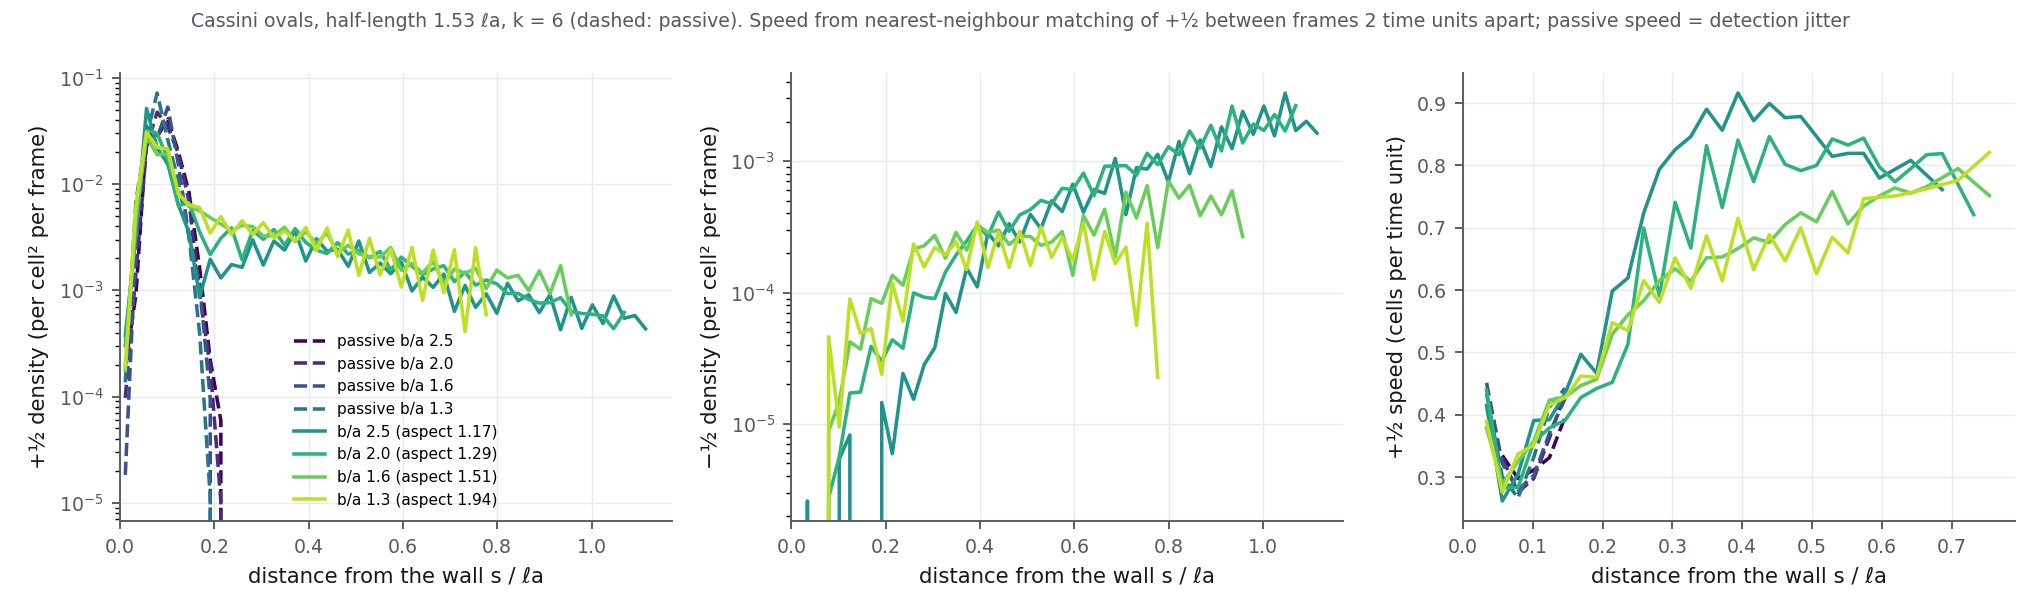
\includegraphics[width=\textwidth]{profiles_ovals_small.png}
\caption{Small ovals: $+\half$ and $-\half$ density and $+\half$ speed against the distance from the wall (dashed: passive).}\label{fig:prof-small}
\end{figure}
\begin{figure}[H]\centering
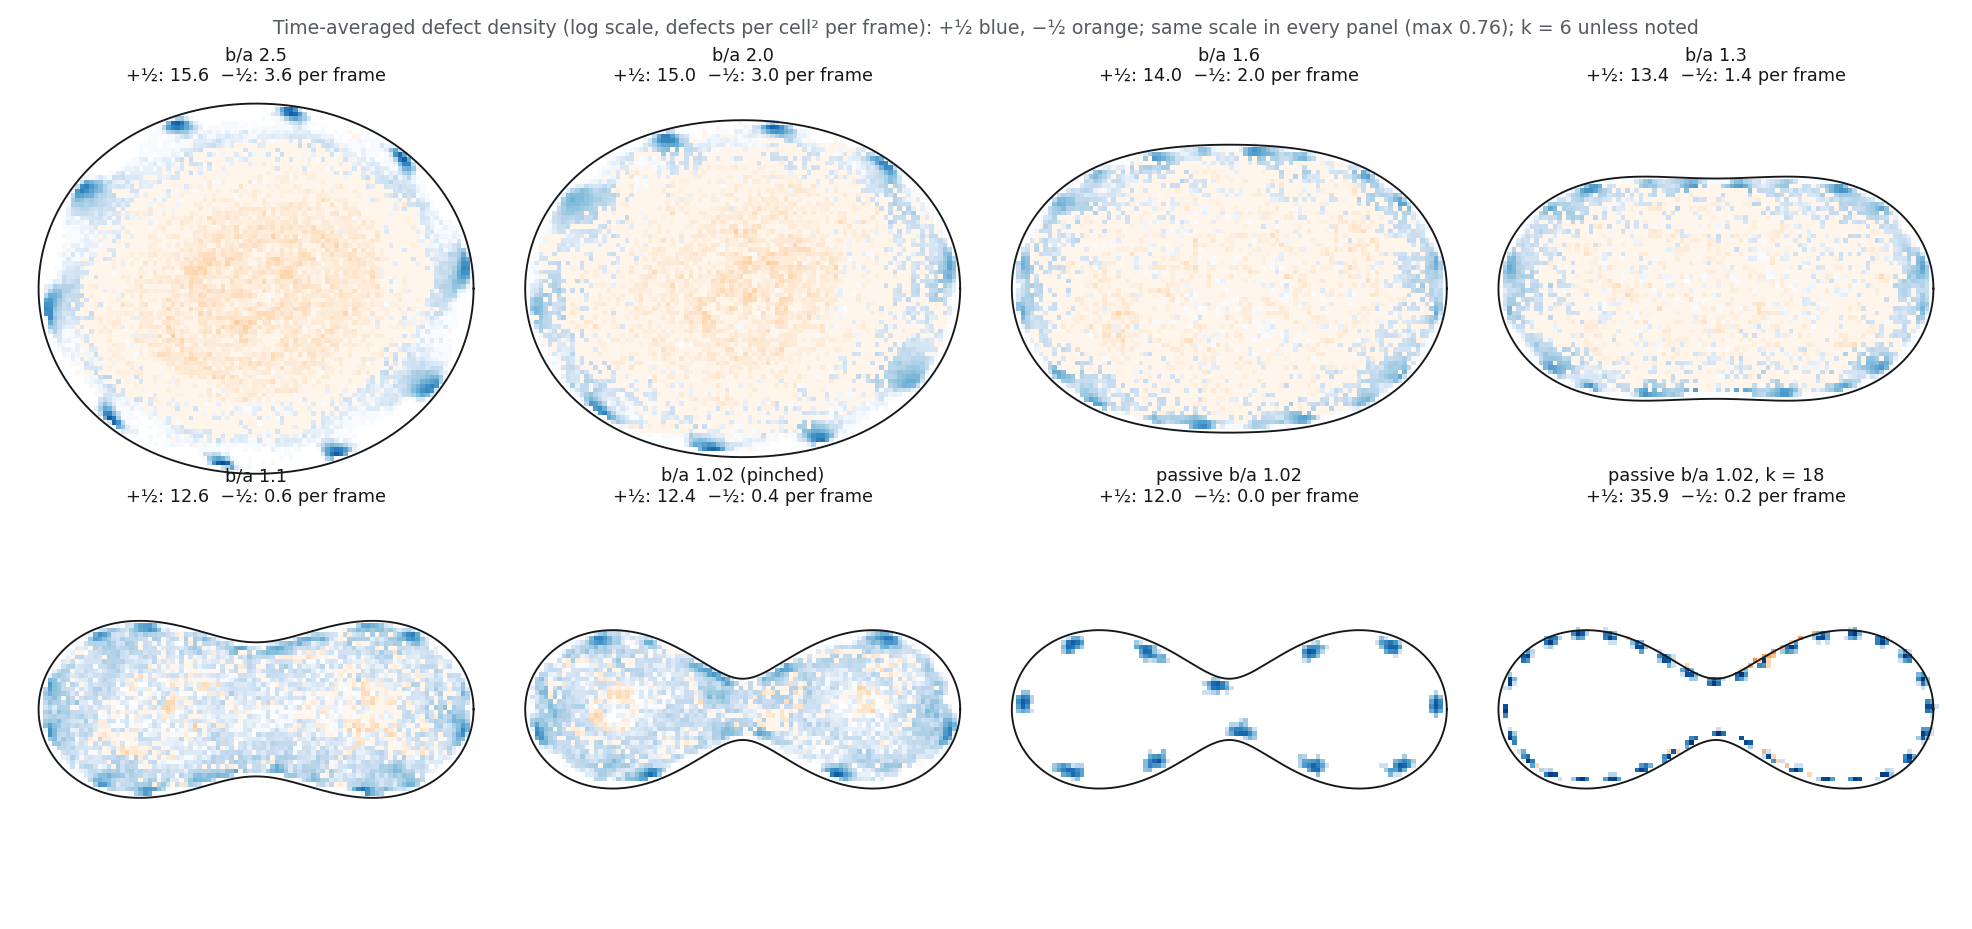
\includegraphics[width=\textwidth]{maps_ovals_large.png}
\caption{Ovals of half-length $2.16\,\la$, $k=6$: $b/a=2.5$, 2.0, 1.6, 1.3, 1.1 and the pinched 1.02 (active), the passive pinched
oval and the passive pinched oval at $k=18$.}\label{fig:maps-large}
\end{figure}
\begin{figure}[H]\centering
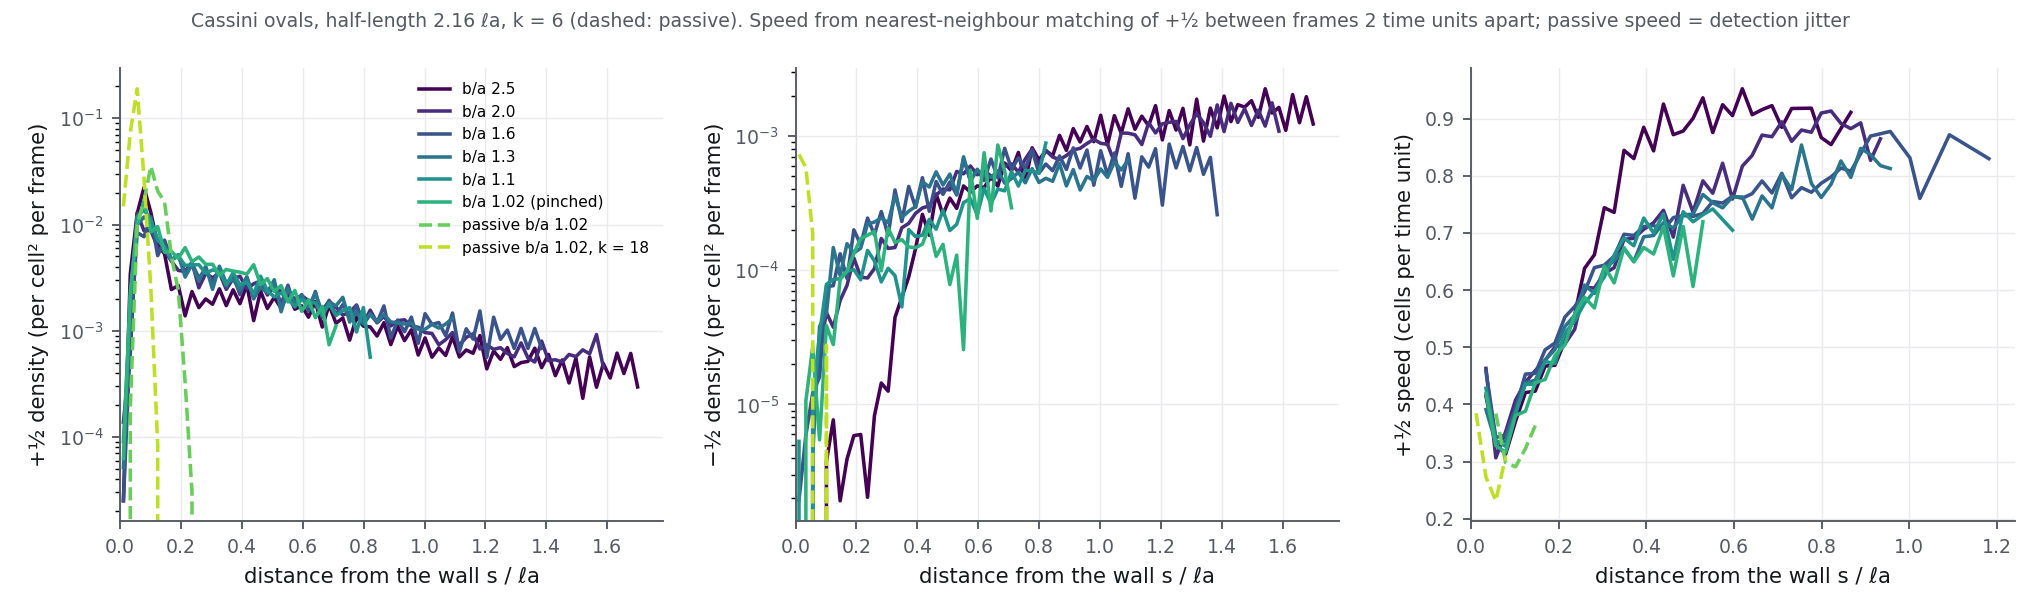
\includegraphics[width=\textwidth]{profiles_ovals_large.png}
\caption{Ovals of half-length $2.16\,\la$: profiles against the distance from the wall (dashed: passive).}\label{fig:prof-large}
\end{figure}
\begin{figure}[H]\centering
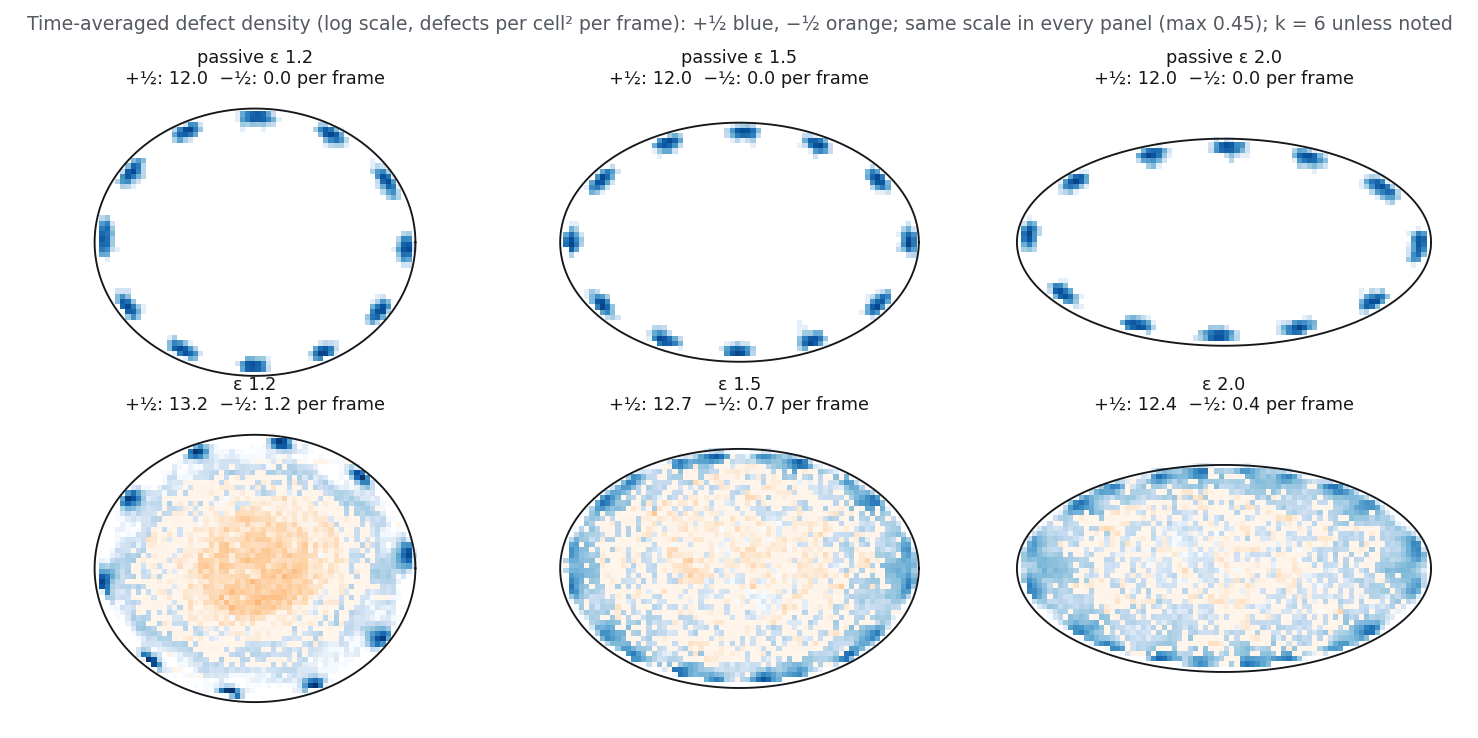
\includegraphics[width=0.92\textwidth]{maps_ellipses.png}
\caption{Ellipses (area 2500, $\sqrt{A/\pi}=1.27\,\la$), $k=6$: passive (top) and active (bottom), $\varepsilon=1.2$, 1.5, 2.0.}\label{fig:maps-ell}
\end{figure}
\begin{figure}[H]\centering
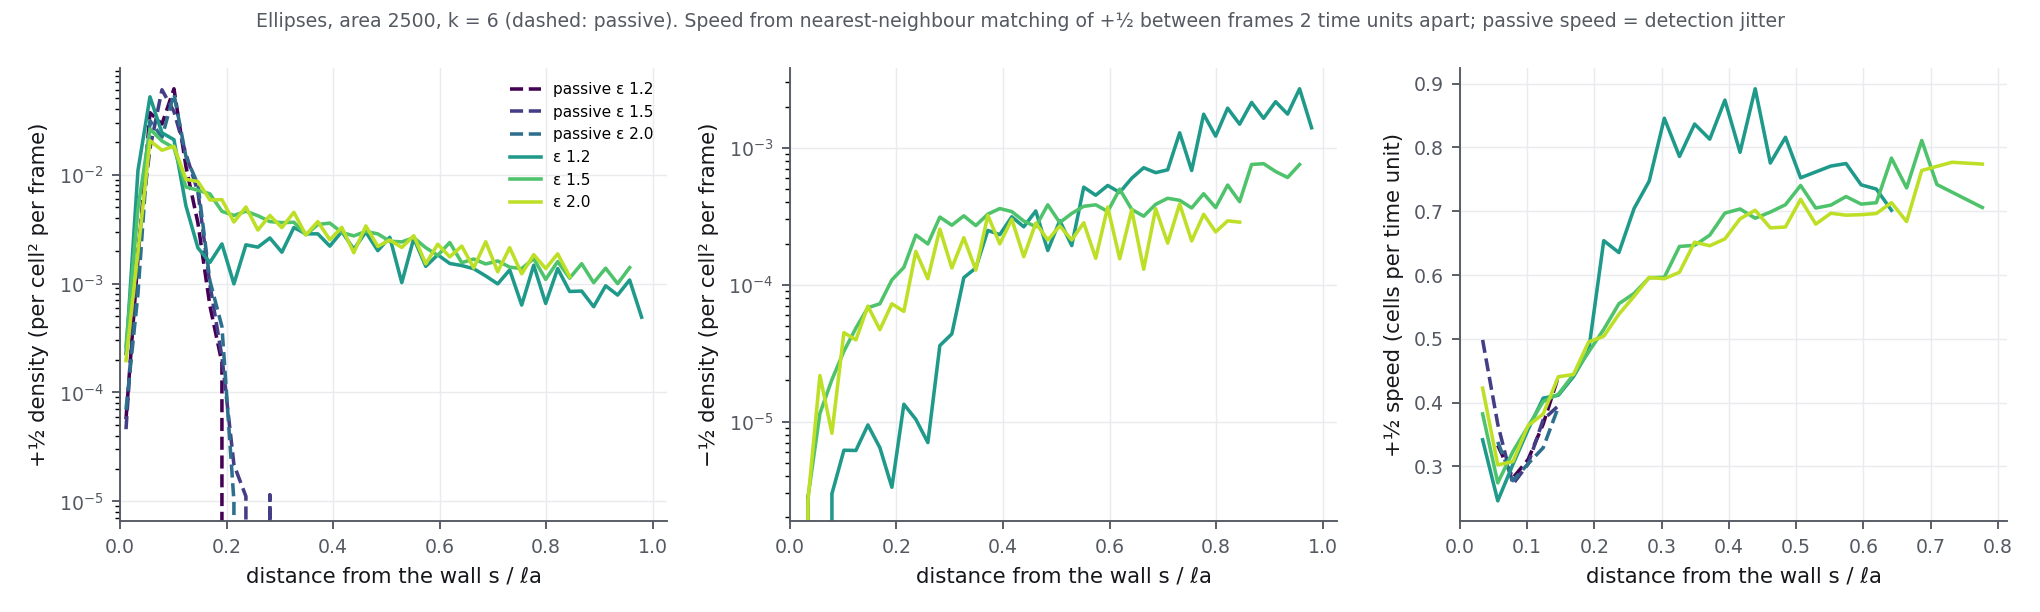
\includegraphics[width=\textwidth]{profiles_ellipses.png}
\caption{Ellipses: profiles against the distance from the wall (dashed: passive).}\label{fig:prof-ell}
\end{figure}
\begin{itemize}
  \item \textbf{Round shapes look like circles}: $b/a=2.5$ (aspect 1.17) and the ellipse $\varepsilon=1.2$ have 10 $=2k-2$ compact wall
        sites, a gap and a bulk with the $-\half$ in the centre.
  \item \textbf{Elongated shapes have no separate layer}: from aspect $\approx1.5$ the wall sites smear into a continuous band (at aspect 1.29 the sites are still discrete in these maps, but
        fewer are occupied; Secs.~\ref{sec:slattice}, \ref{sec:ssurv}),
        $+\half$ density rises steadily towards the wall without a gap, and far fewer $-\half$ are created (e.g.\ half-length
        $2.16\,\la$: 3.6 $-\half$ per frame at $b/a=2.5$, 2.0 at 1.6, 1.4 at 1.3, 0.4 in the pinched oval; the circle of the same
        half-length has 4.7). The $-\half$ no longer concentrate in one centre.
  \item In the pinched ovals defects accumulate at the neck, and each lobe has its own weak $-\half$ centre.
\end{itemize}
\begin{figure}[H]\centering
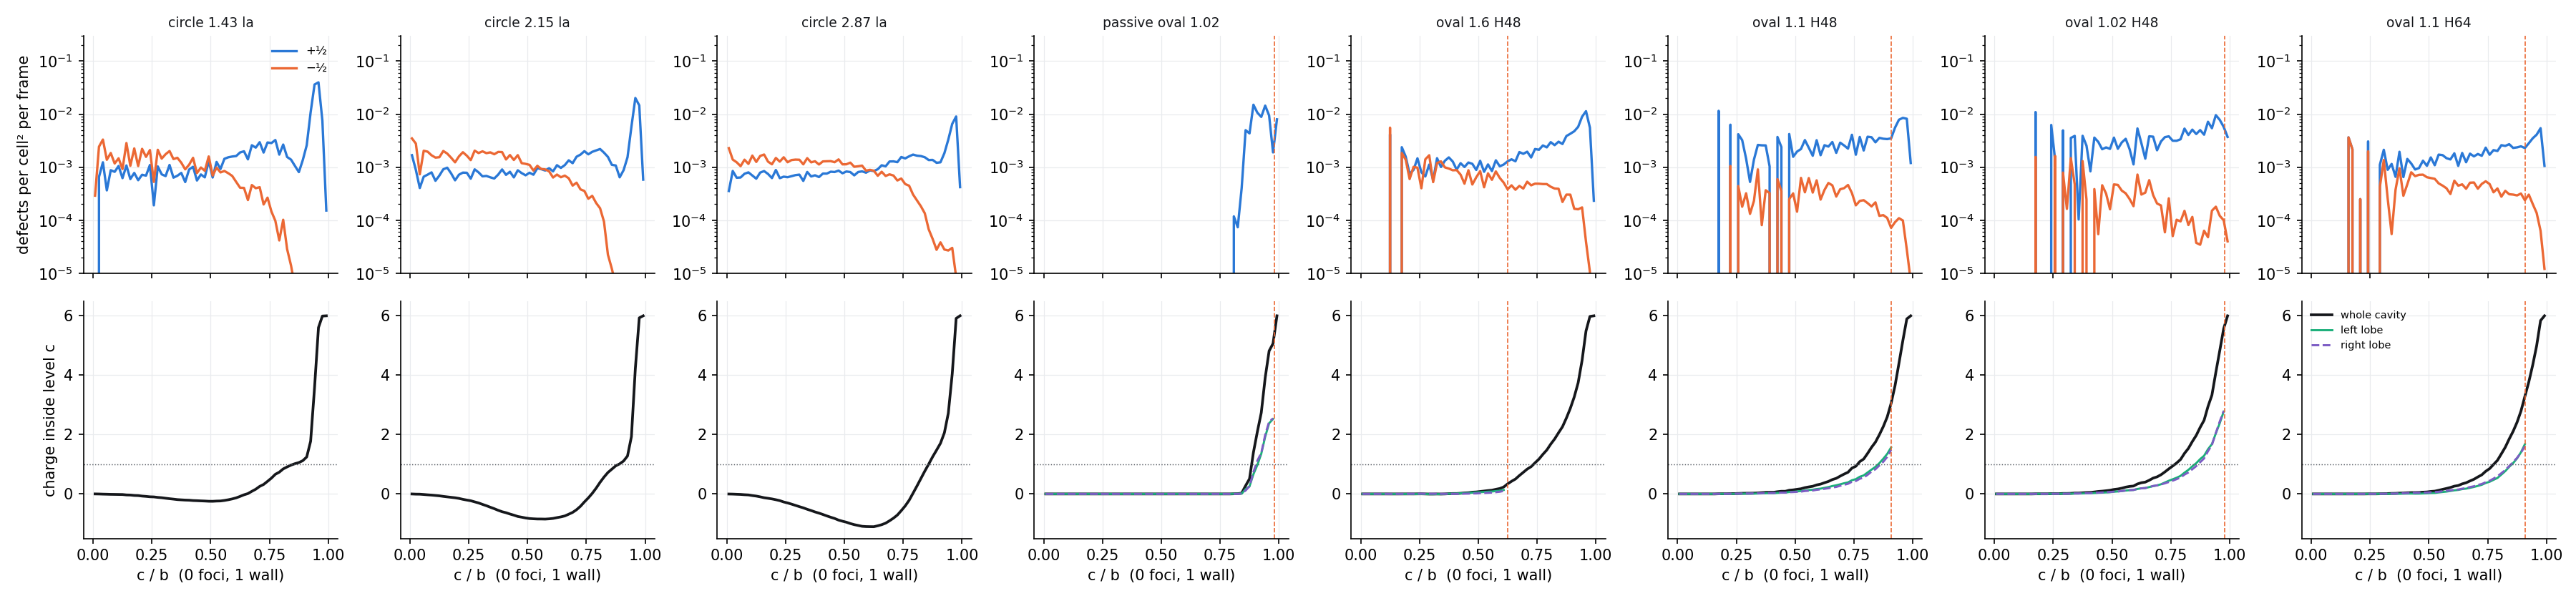
\includegraphics[width=\textwidth]{lobe_profiles_large.png}
\caption{Defect densities and accumulated charge in Cassini level coordinates $c=\sqrt{d_1d_2}$ (0 at the foci, $b$ at the wall)
for circles ($k=6$; 1.43, 2.15, $2.87\,\la$) and ovals of half-length 2.16 and $2.88\,\la$ (1 seed). Circles: $+\half$ wall peak at
$c/b\approx0.97$, dip inside it, negative $Q$ towards the centre. Ovals: $n_+$ rises steadily, no peak--gap structure.}\label{fig:lobeprof}
\end{figure}
\begin{figure}[H]\centering
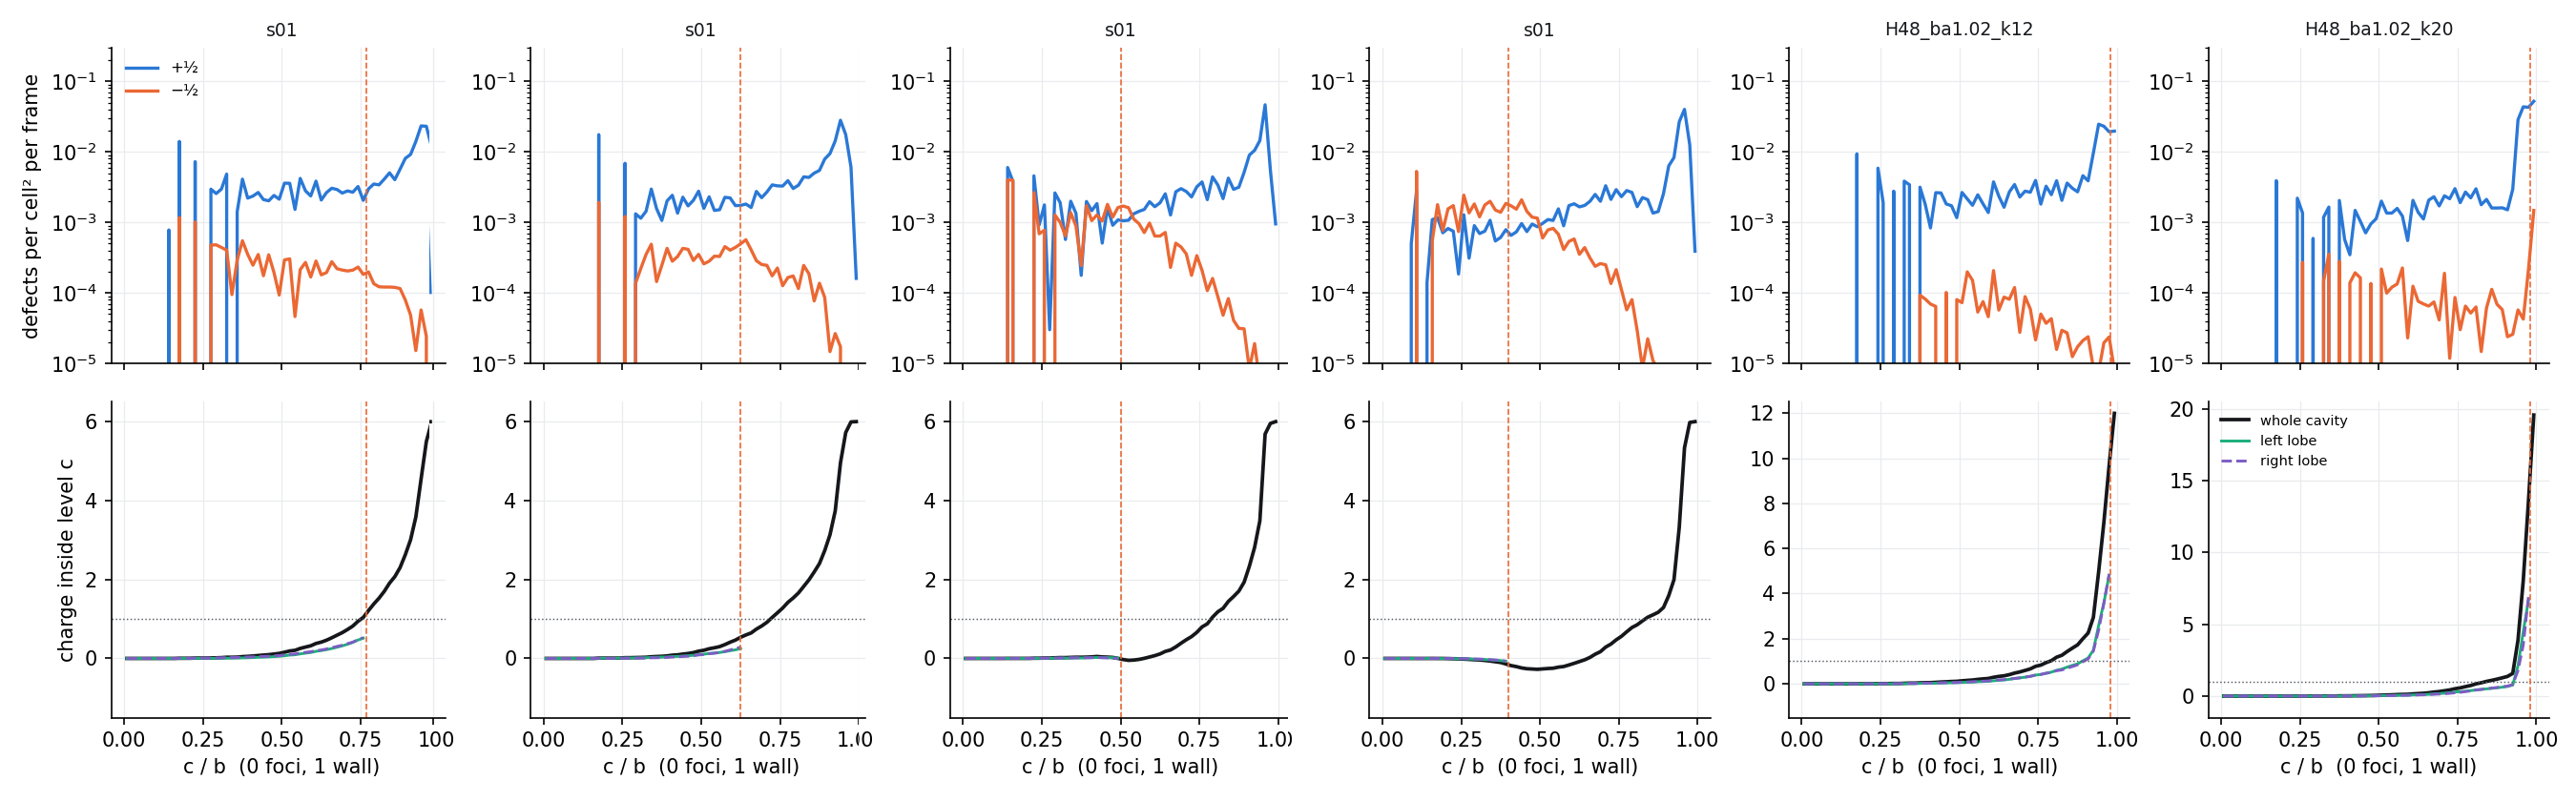
\includegraphics[width=\textwidth]{lobe_profiles_small_sel.png}
\caption{The same in level coordinates for seed 1 of the small ovals ($b/a=1.3$, 1.6, 2.0, 2.5; red line: lemniscate level $c=a$) and the pinched
oval at $k=12$, 20 (whole cavity and per-lobe $Q$). Top: $+\half$ (blue) and $-\half$ (orange) density; bottom: $Q(c)$.}\label{fig:lobeprof-small}
\end{figure}
\begin{figure}[H]\centering
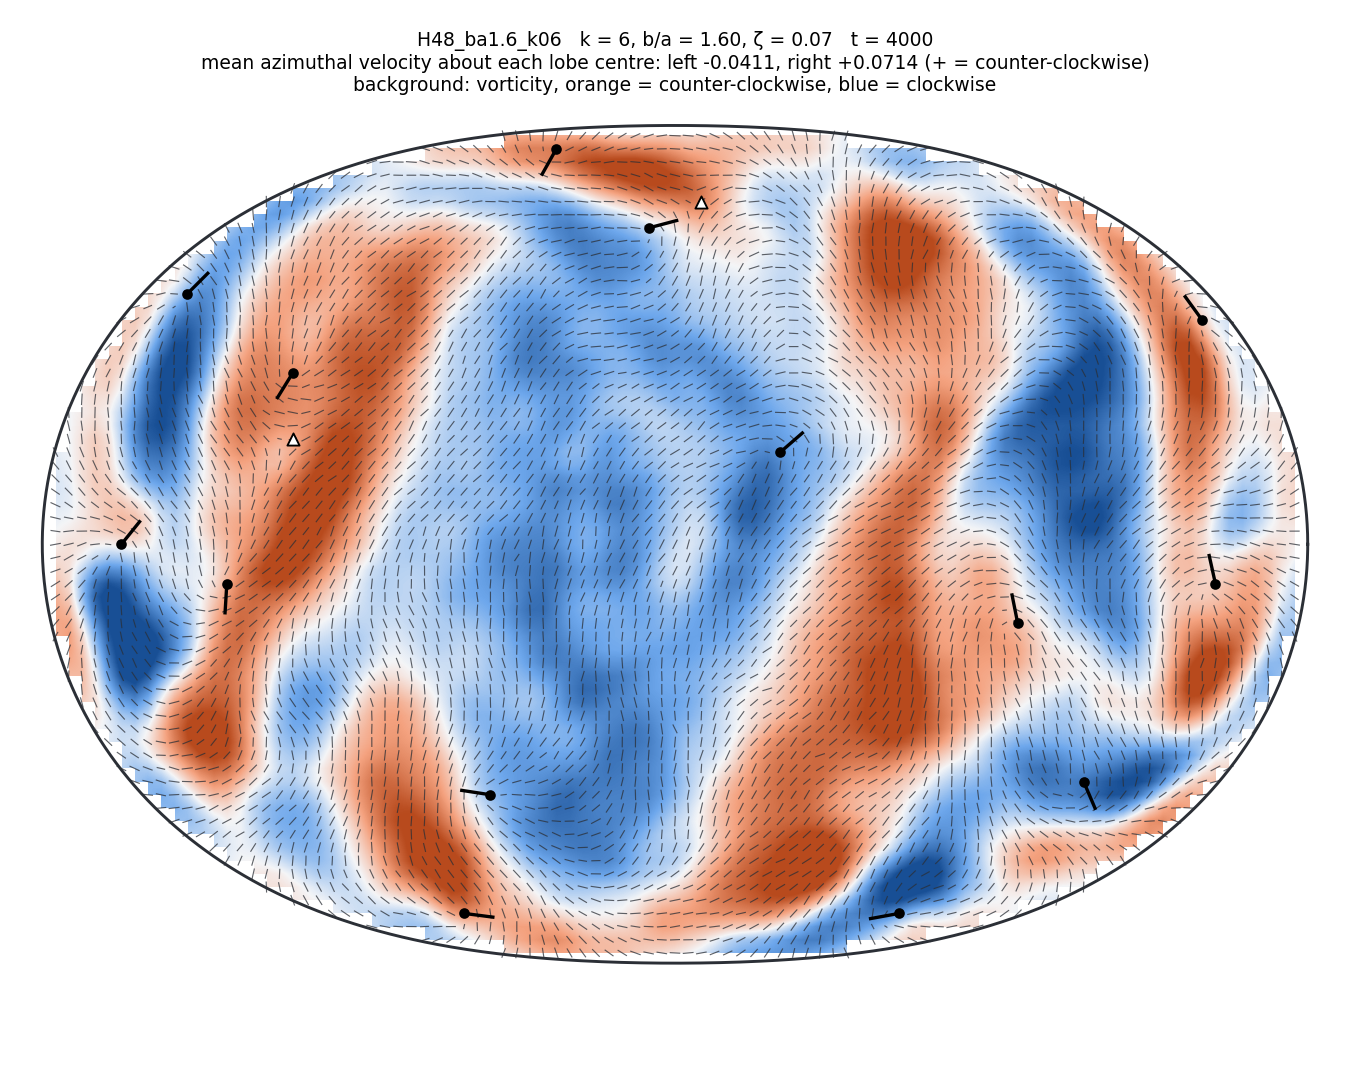
\includegraphics[width=0.49\textwidth]{snap_ba1.6.png}\hfill
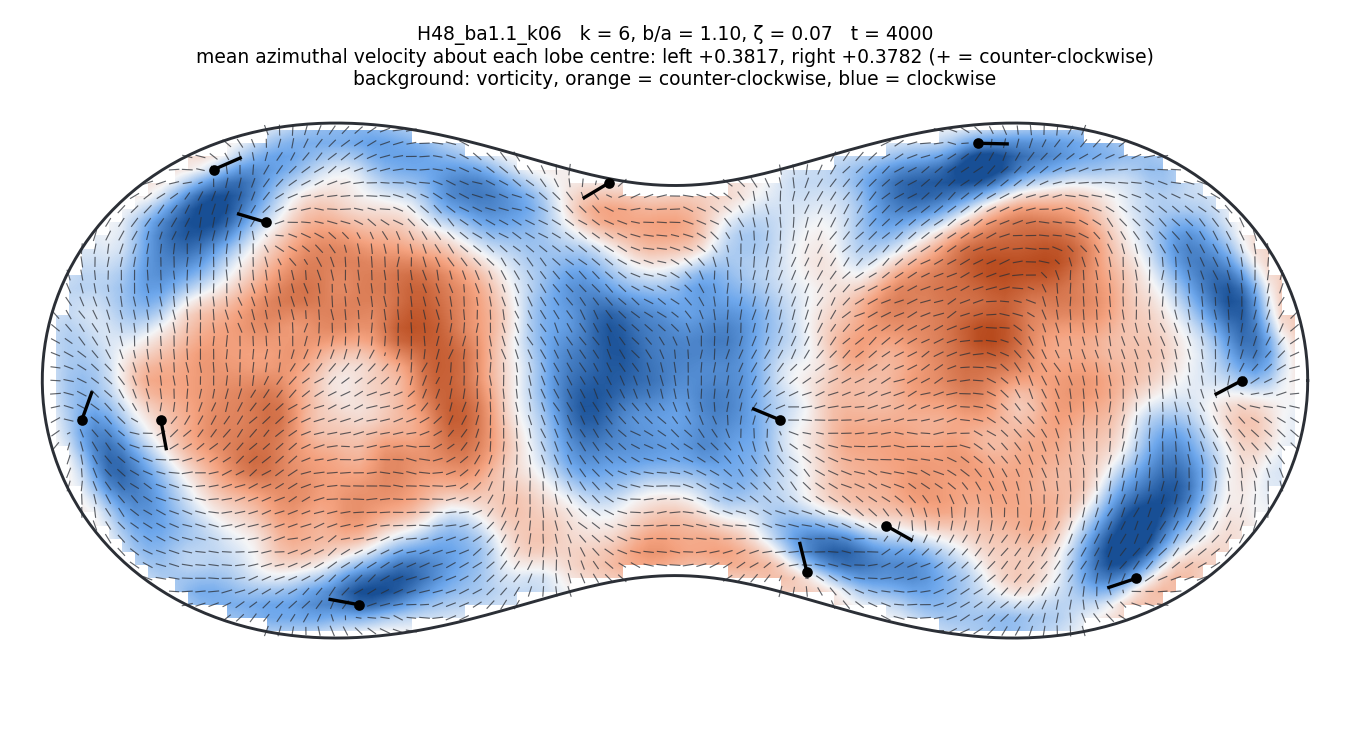
\includegraphics[width=0.49\textwidth]{snap_ba1.1.png}\\[4pt]
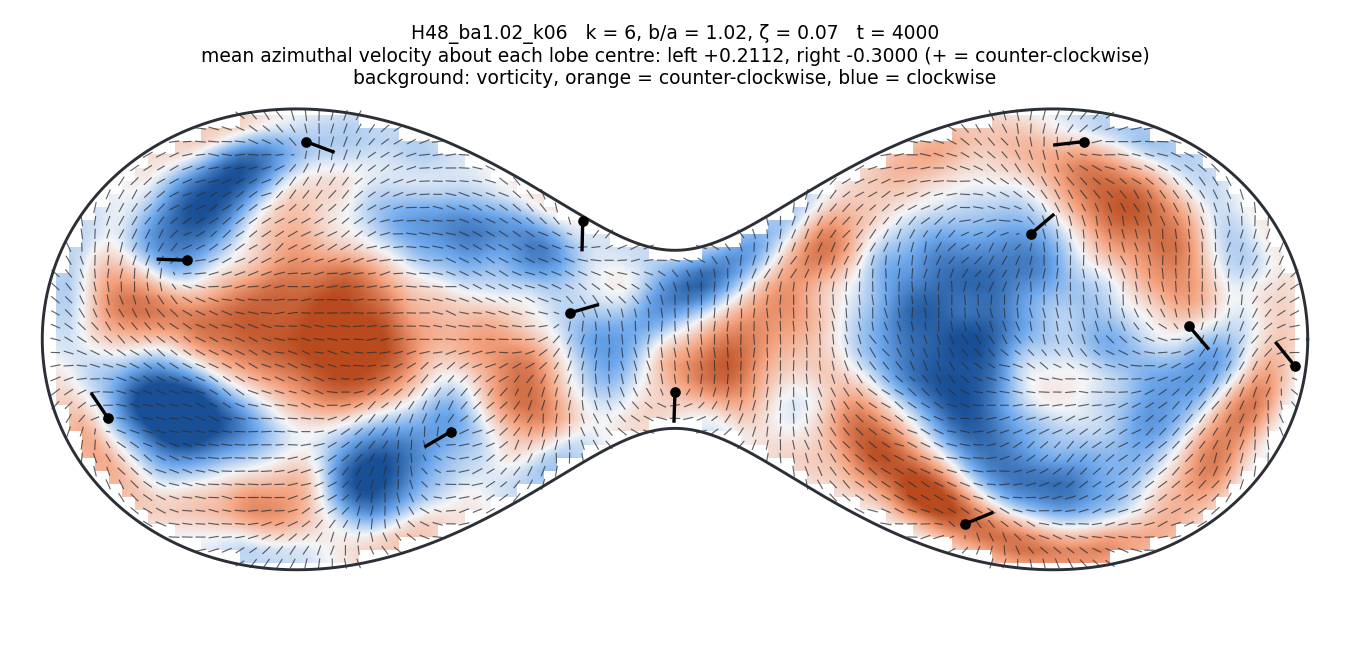
\includegraphics[width=0.49\textwidth]{snap_ba1.02.png}\hfill
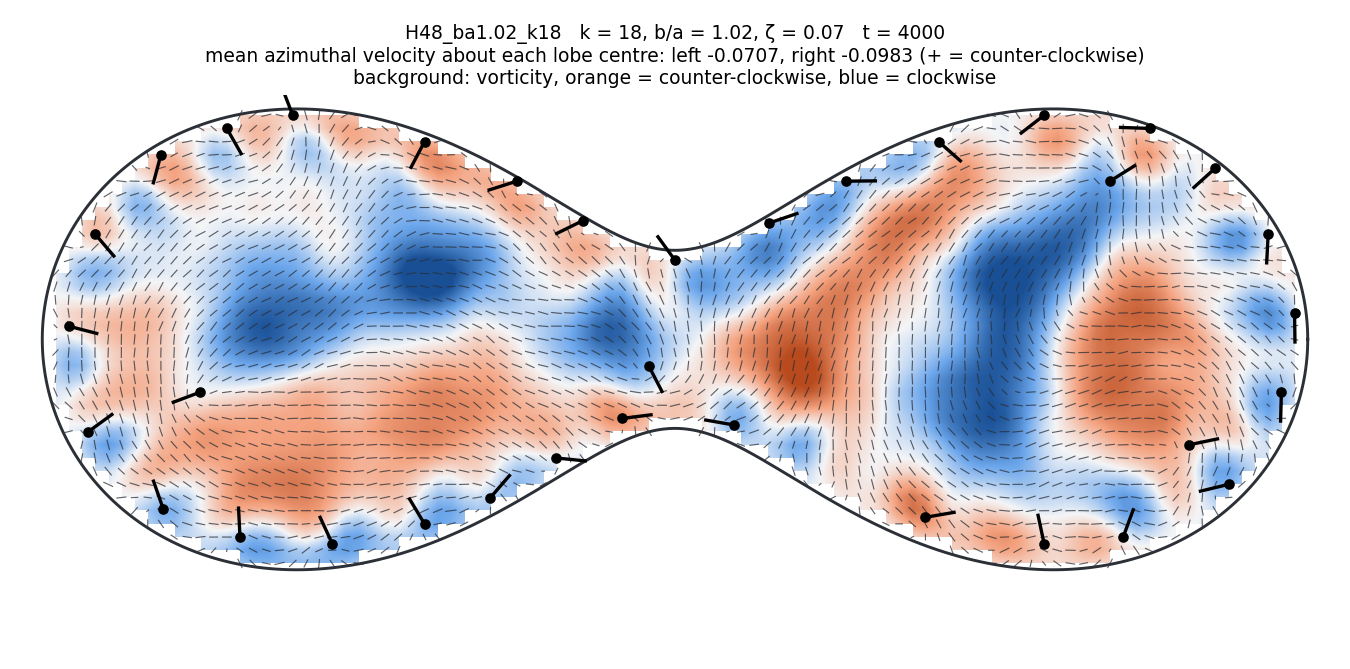
\includegraphics[width=0.49\textwidth]{snap_ba1.02_k18.png}
\caption{Snapshots at the end of the runs (half-length $2.16\,\la$): vorticity (orange counter-clockwise, blue clockwise), director,
$+\half$ (dots with orientation tail), $-\half$ (triangles). $b/a=1.6$, 1.1, 1.02 ($k=6$) and 1.02 at $k=18$. Movies:
\texttt{results/6\_shape/movies/}.}\label{fig:snaps}
\end{figure}

%=====================================================================
\section{The charge split in ovals and ellipses}\label{sec:scharge}
\subsection{Accumulated charge: plateau or not}
The accumulated charge $Q(c)$ inside the level $c$ (circle: $c=r$; Cassini: $c=\sqrt{d_1d_2}$; ellipse: scaled copies of the wall)
is the cut-free observable (Sec.~\ref{sec:methods-Q}).
\begin{figure}[H]\centering
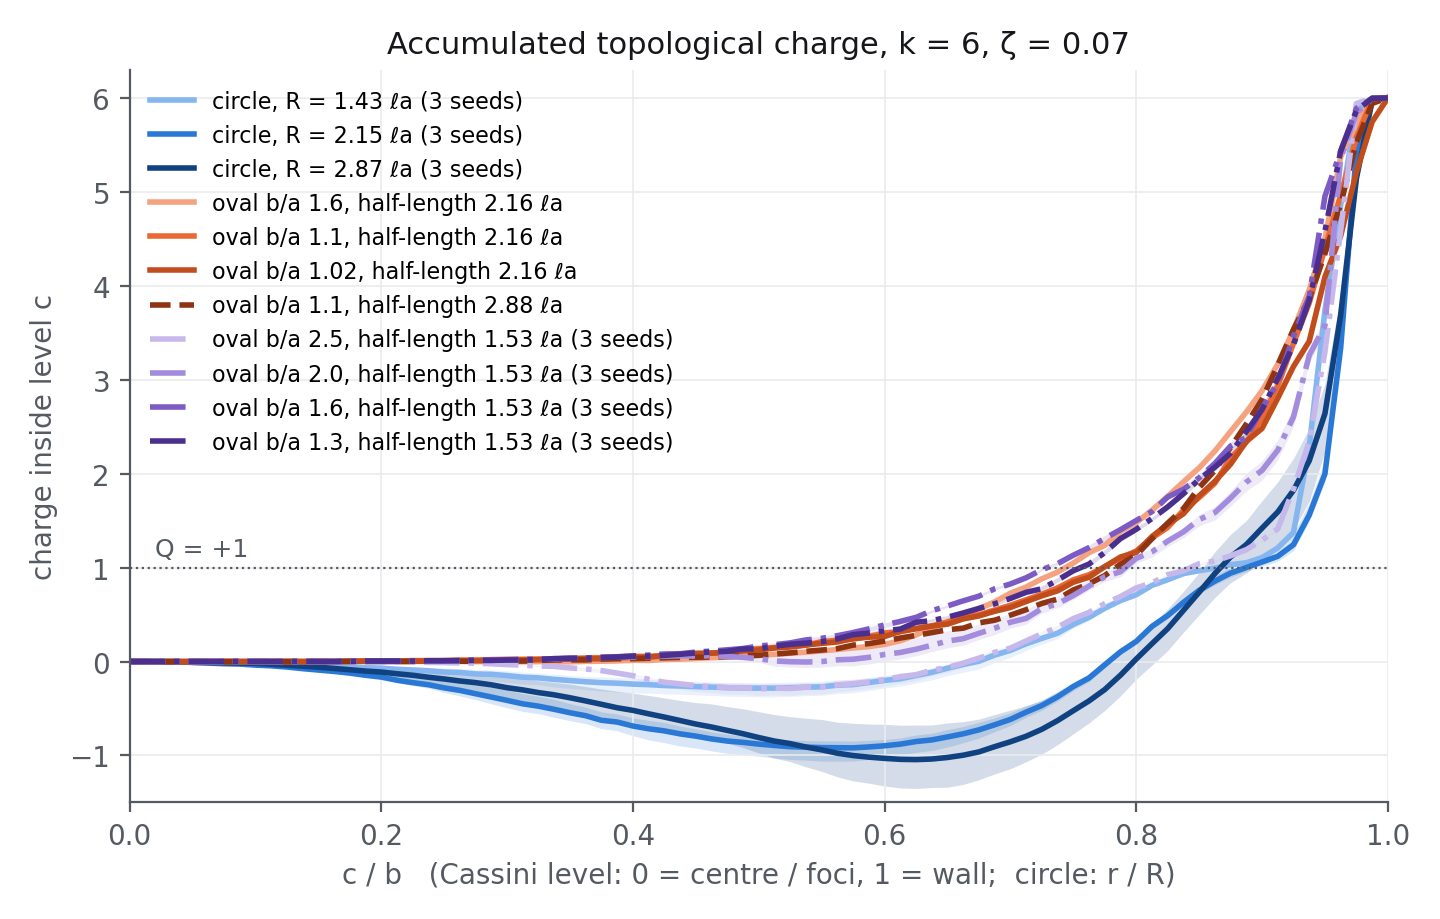
\includegraphics[width=0.85\textwidth]{accumulated_charge.png}
\caption{\textbf{Accumulated charge inside level $c$} ($k=6$, $\zeta=0.07$). Circles (mean of 3 seeds, min--max band): negative
dip ($-\half$ core), plateau at $+1$ for $c/b\approx0.85$--0.93, jump to $k$ within the last few percent (the layer). Ovals of
half-length 2.16 and $2.88\,\la$: monotonic, never negative, no plateau, crossing $+1$ at $c/b\approx0.78$, all on nearly one
curve. Small ovals (half-length $1.53\,\la$, 3 seeds; dash-dotted, light to dark = $b/a$ 2.5 to 1.3): $b/a=2.5$ follows the
circles.}\label{fig:Qc}
\end{figure}

\subsection{Size control: small ovals at half-length $1.53\,\la$}
Four shapes at the size where circles are cleanest, 3 seeds each:
\begin{table}[H]\centering\small
\caption{Small ovals compared with circles of comparable size, all measures. Criteria agree: fraction of $+\half$ on which
mobility and tilt agree with the site rule.}\label{tab:p3}
\begin{adjustbox}{max width=\textwidth}
\begin{tabular}{lccccccc}\toprule
cavity & aspect & sites & $q_b$ (site rule) & labels at wall after 1000 & criteria agree & $d^*/\la$ & $f^*$\\\midrule
circle $R=1.43\,\la$ & 1 & 10 & 1.01--1.05 & 0.87--0.94 & 97--99\% & 0.19--0.20 & 0.26\\
oval $b/a=2.5$ & 1.17 & 10 & 1.07--1.11 & 0.82--0.86 & 97--98\% & 0.22--0.23 & 0.29\\
oval $b/a=2.0$ & 1.29 & 8--9 & 1.6--2.1 & 0.60--0.65 & 81--86\% & 0.29--0.31 & 0.39\\
oval $b/a=1.6$ & 1.51 & (3--7) & 3.3--3.5 & 0.37--0.40 & 72--74\% & 0.41 & 0.53\\
oval $b/a=1.3$ & 1.94 & (3--7) & 3.3--3.6 & 0.42--0.50 & 69--72\% & 0.49--0.50 & 0.63\\\bottomrule
\end{tabular}
\end{adjustbox}
\end{table}
\begin{itemize}
  \item \textbf{Sharp crossover with elongation at fixed size and density:} circle-like at aspect 1.17 ($2k-2$ pinned sites, bulk $+1$,
        wall defects stay), partial at 1.29, lost from $\approx1.4$ while the shape is still convex ($b/a=1.6>\sqrt2$).
  \item In the elongated ovals the site rule finds only a few unstable sites; any cut-free criterion (mobility, tilt or both) gives a
        bulk of 3.1--3.9 (only $\approx4$--5.5 of the 12 imposed $+\half$ behave like wall defects), against 1.1--1.25 in circles of
        the same half-length (Table~\ref{tab:edgeovals}).
\end{itemize}
\begin{table}[H]\centering\small
\caption{Bulk charge $q_b=k-(\text{edge-like})/2$ from the cut-free criteria, $k=6$ (1 seed for the larger ovals).}\label{tab:edgeovals}
\begin{adjustbox}{max width=\textwidth}
\begin{tabular}{lccc}\toprule
cavity & tilted & slow & slow and tilted\\\midrule
circle $1.43\,\la$ (site rule 1.05) & 1.07 & 1.05 & 1.06\\
circle $2.15\,\la$ & 1.11 & 1.25 & 1.24\\
circle $2.87\,\la$ (site rule 1.85) & 1.93 & 2.71 & 2.66\\
ovals half-length $2.16\,\la$, $b/a=1.6$ / 1.1 / 1.02 & 3.42 / 3.58 / 3.26 & 3.66 / 3.44 / 3.10 & 3.85 / 3.87 / 3.57\\
oval half-length $2.88\,\la$, $b/a=1.1$ & 4.03 & 4.25 & 4.45\\\bottomrule
\end{tabular}
\end{adjustbox}
\end{table}
\begin{figure}[H]\centering
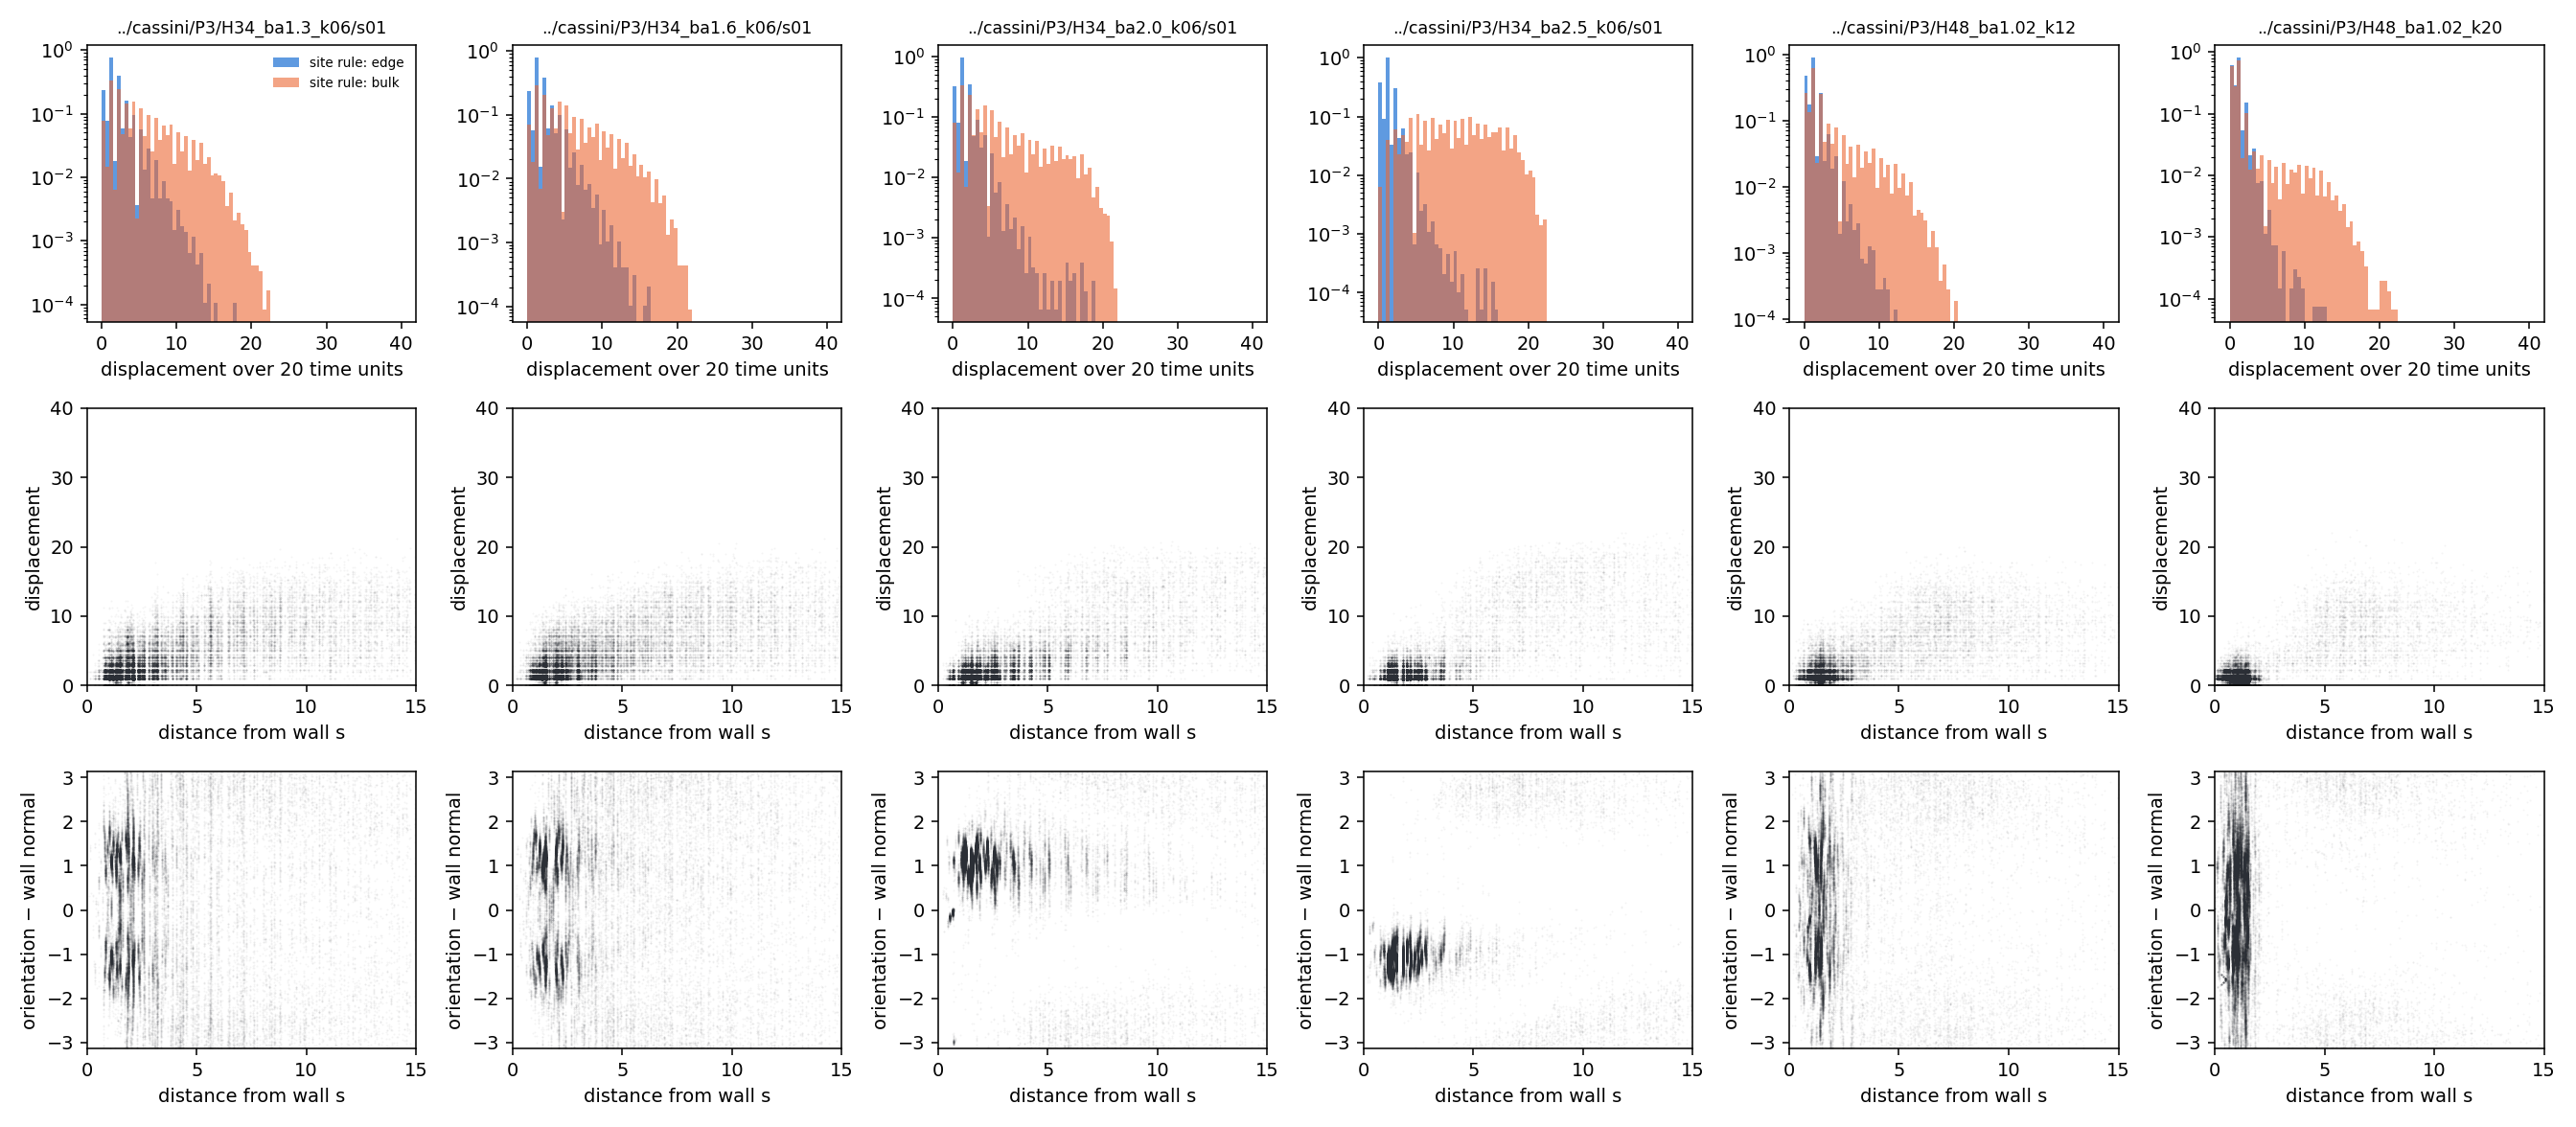
\includegraphics[width=\textwidth]{edge_criteria_small_sel.png}
\caption{Cut-free criteria, seed 1 of each small oval ($b/a=1.3$, 1.6, 2.0, 2.5) and the pinched oval at $k=12$ and 20. Top: displacement over
20 time units (blue: on a site, orange: bulk, by the site rule); middle: displacement against the distance from the wall; bottom:
orientation relative to the outward wall normal against the distance from the wall. Round ovals: wall defects tilted at $\approx\pm1.1$ rad with
one sign (the single vortex). Elongated ovals: both signs, one per lobe vortex. Crowded pinched oval ($k=20$): tilt close to 0, as in
high-density circles. All 16 runs: \texttt{results/6\_shape/small\_ovals\_1.53la/edge\_criteria.png}.}\label{fig:critsmall}
\end{figure}

\subsection{One number per cavity: layer depth $d^*$ and area fraction $f^*$}
$c^*$ = outermost level where $Q$ crosses $+1$; $d^*$ = mean wall distance along that level (circle: $R-c^*$);
$f^*=A(c>c^*)/A$, the fraction of the cavity between the $Q=+1$ level and the wall (Sec.~\ref{sec:methods-dstar}). For a true
layer of fixed width $f^*$ falls as the cavity grows; for charge spread through the cavity $f^*$ is set by the shape alone.
Beyond $f^*=\half$ the ``layer'' would be larger than the bulk it surrounds.
\begin{figure}[H]\centering
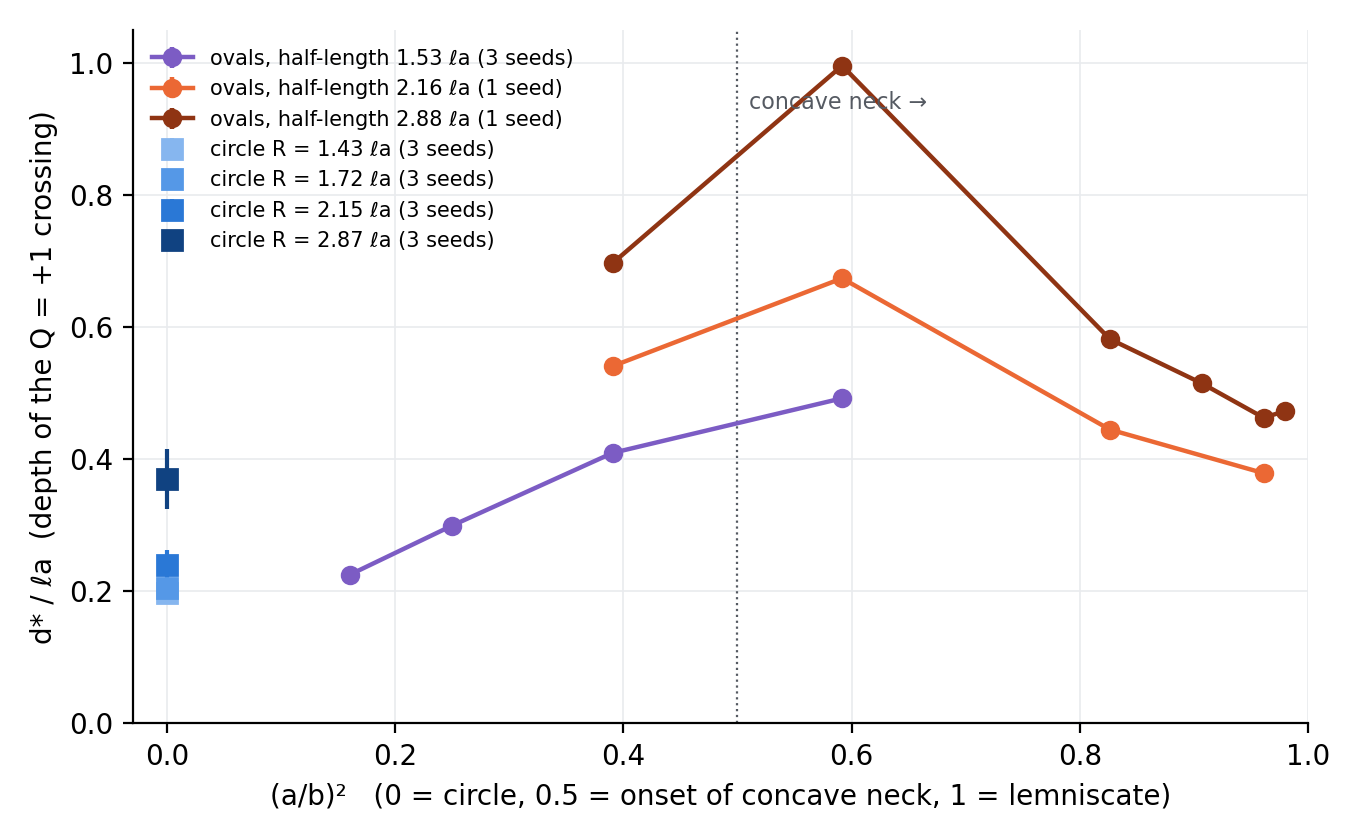
\includegraphics[width=0.82\textwidth]{layer_depth.png}
\caption{Layer depth $d^*/\la$ against elongation $(a/b)^2$ (0 circle, 0.5 onset of the concave neck, 1 lemniscate), $k=6$.
Squares: circles 1.43--$2.87\,\la$. Small ovals (3 seeds) rise from 0.23 to 0.50; larger ovals (1 seed) peak near $b/a\approx1.3$.}\label{fig:dstar}
\end{figure}
\begin{figure}[H]\centering
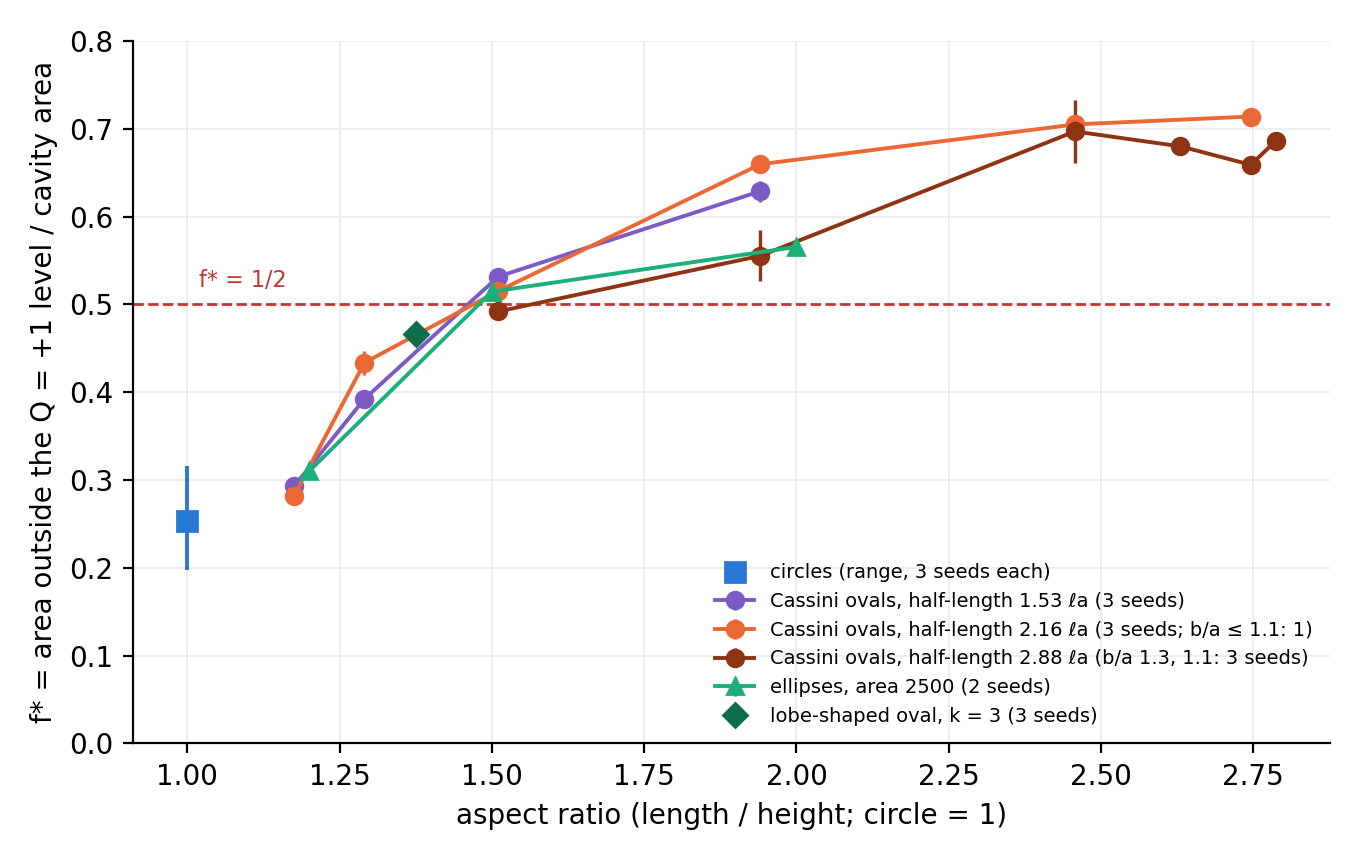
\includegraphics[width=0.85\textwidth]{layer_area_all.png}
\caption{\textbf{Area fraction $f^*$ outside the $Q=+1$ level against the aspect ratio}, all shapes with seeds: Cassini ovals at
three sizes, ellipses (area 2500), the lobe-shaped oval, circles (range over 1.08--$2.15\,\la$, $k=3$ and 6). Dashed: $f^*=\half$.}\label{fig:fstar}
\end{figure}
\begin{itemize}
  \item \textbf{Circles:} $d^*\approx4.5$--6 cells $\approx0.2\,\la$ up to $2.15\,\la$ (0.31--0.42 at $2.87\,\la$); $f^*=0.20$--0.32, falling
        with size (0.26 at 1.43, 0.20 at $2.15\,\la$): a layer of fixed width.
  \item \textbf{Same size, different shape:} at half-length $1.53\,\la$, $d^*/\la=0.23\to0.30\to0.41\to0.50$ for $b/a=2.5\to1.3$.
  \item \textbf{$f^*$ collapses on the aspect ratio for all oval sizes} (half-length 1.53 / 2.16\,$\la$, 3 seeds: $b/a=2.5$: 0.29 / 0.28;
        2.0: 0.39 / 0.42--0.45; 1.6: 0.53 / 0.49--0.54; 1.3: 0.63 / 0.65--0.67), crossing $\half$ near aspect 1.5 and levelling at
        0.65--0.7. At $2.88\,\la$ slightly lower ($\approx0.56$ at aspect 1.94): good but not perfect collapse.
  \item \textbf{Ellipses follow the same curve:} $\varepsilon=1.2$: knee 0.98--1.07, $f^*=0.31$, pinned lattice; 1.5: no knee, $f^*=0.51$--0.52;
        2.0: no knee, $f^*=0.57$ (Table~\ref{tab:ell}). A convex cavity can lose the layer; elongation is the control for both families.
  \item The size independence of $f^*$ is itself the diagnostic of ``no layer''. The equivalent strip width
        $w_\mathrm{eff}=A(c>c^*)/P$ is $0.17$--$0.25\,\la$ for every clean circle layer and grows with size in ovals.
\end{itemize}
\begin{table}[H]\centering\small
\caption{Ellipses (2 seeds): $Q$ at fixed levels, knee and $f^*$.}\label{tab:ell}
\begin{adjustbox}{max width=\textwidth}
\begin{tabular}{lccccc}\toprule
& $Q(0.80)$ & $Q(0.85)$ & $Q(0.90)$ & knee & $f^*$\\\midrule
$\varepsilon=1.2$ & 0.88--0.90 & 1.05--1.07 & 1.32--1.34 & 0.98--1.07 & 0.31\\
$\varepsilon=1.5$ & 1.64--1.68 & 2.10--2.13 & 2.96--2.98 & none & 0.51--0.52\\
$\varepsilon=2.0$ & 1.93--1.95 & 2.46--2.49 & 3.47--3.48 & none & 0.57\\\bottomrule
\end{tabular}
\end{adjustbox}
\end{table}
% NOTE: d* for ellipses is not quoted: layer_depth.py treats an ellipse as a circle of radius R (see Appendix B); f* is unaffected.

\subsection{Not the neck: pinch-off and a lobe-shaped oval}
\begin{itemize}
  \item In the larger ovals $d^*$ falls again as the neck closes ($b/a\to1$). This is \textbf{not} a restored layer: in the tightest necks
        ($b/a=1.01$--1.05) each lobe's charge passes $+1$ about 10 cells from the wall with slope $\mathrm{d}Q/\mathrm{d}(c/b)\approx8$--10
        (circle plateau $\approx3$, circle layer jump 50--100), the whole cavity passes $+2$ without a plateau, and $Q_L\approx Q_R$. The
        lobes are just smaller.
  \item Circles with the area of one lobe and half the winding ($k=3$, $R=1.08$ and $1.43\,\la$, 3 seeds) keep a normal layer
        ($d^*=4.1$--5.0 cells, $+1$ plateau). A lobe does not behave like a circle of its size, even with a 13-cell neck.
  \item \textbf{A single convex oval with the area and aspect of one lobe} ($b/a=1.8$, aspect 1.38, $k=3$, 3 seeds) loses the layer too:
        3 sites instead of $2k-2=4$, $q_b\approx1.9$ of 3, $d^*/\la=0.31$--0.32 (circles of the same area 0.18--0.22), $Q(c)$ smooth,
        only 16--28\% of the wall labels at the wall after 1000. The lobe shape is enough; no coupling through the neck is needed.
\end{itemize}

\subsection{The winding: crowded walls push back}
\begin{table}[H]\centering\small
\caption{$k$ scan at half-length $1.53\,\la$ (3 seeds): $Q$ at the fixed level $c/b=0.85$ (no knee needed); in brackets the knees
found (seeds) and their value.}\label{tab:kscan}
\begin{adjustbox}{max width=\textwidth}
\begin{tabular}{lcccccc}\toprule
& $k=2$ & 4 & 6 & 8 & 10 & 12\\\midrule
circle $R=1.43\,\la$ & 0.99 & 0.95 & 0.95 & 0.94 & 0.97 & --\\
oval $b/a=2.0$ & 1.12 & 1.54 & 1.51 & 1.49 & 1.36 & 1.24 (3/3, 1.31)\\
oval $b/a=1.6$ & 1.30 & 2.06 & 1.96 & 1.63 & 1.42 (1/3, 1.54) & 1.31 (3/3, 1.40)\\\bottomrule
\end{tabular}
\end{adjustbox}
\end{table}
\begin{figure}[H]\centering
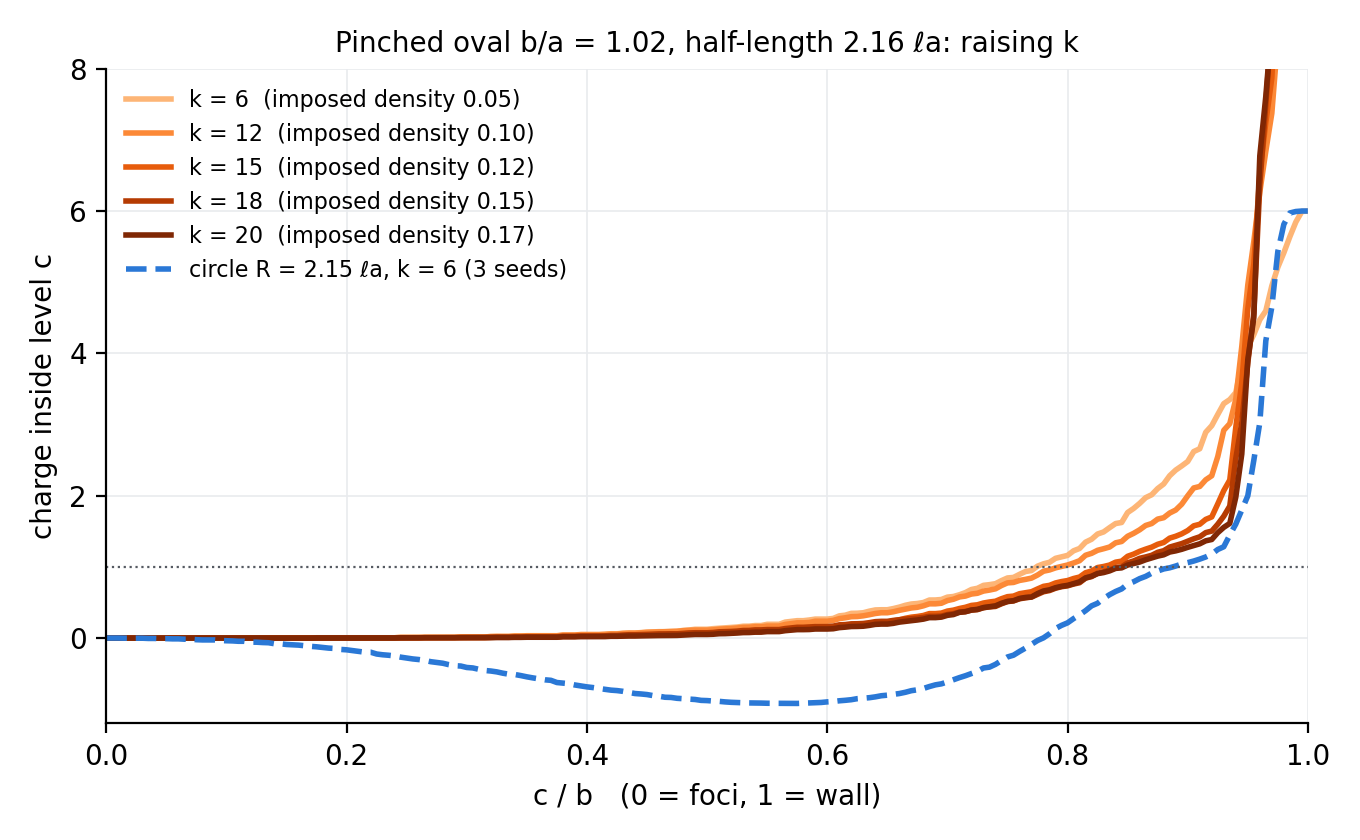
\includegraphics[width=0.82\textwidth]{highk.png}
\caption{Accumulated charge in the pinched oval ($b/a=1.02$, half-length $2.16\,\la$) for $k=6$ to 20 (imposed density 0.05 to 0.17), with
the circle of $R=2.15\,\la$ for reference.}\label{fig:highk}
\end{figure}
\begin{itemize}
  \item \textbf{Circle: a traditional layer}, $Q$ at fixed depth independent of $k$ (slope $-0.002$ per unit $k$): all extra winding goes
        to the wall.
  \item \textbf{Ovals: a bounded, non-monotonic excess.} The bulk carries at most $\approx+1$ extra at moderate $k$ ($\rho\approx0.04$--0.07),
        and the excess shrinks again as the wall gets crowded; at $k=12$ ($\rho\approx0.13$) a plateau and a wall lattice reappear
        ($f_\mathrm{static}$ for $b/a=1.6$: 0.03, 0.21, 0.11, 0.39, 0.70 for $k=2\dots12$, 1 seed).
  \item \textbf{Pinched oval at high $k$:} $Q(c/b=0.85)$ falls from 1.76 ($k=6$) to 1.03--1.06 ($k=18$, 20), $d^*/\la$ from 0.38 to 0.30
        (circle 0.20), labels stay at the wall (84\% after 1000 at $k=15$, 18). The bulk carries $\approx+1$ \emph{for the whole cavity},
        $\approx+\half$ per lobe, not $+1$ per lobe. 1 seed; $k=18$--20 at the edge of the anchoring resolution.
  \item Same trend as the mirror runs (Sec.~\ref{sec:mirror}): \textbf{a crowded wall favours the topological structure}; elongation
        matters most at moderate imposed density.
\end{itemize}

%=====================================================================
\section{The wall lattice in ovals and ellipses}\label{sec:slattice}
Same analysis as Sec.~\ref{sec:clattice}, with positions measured by arclength along the real wall (Secs.~\ref{sec:md-fourier-static},
\ref{sec:md-fourier-dyn}, \ref{sec:md-drift}); 81 active oval and ellipse runs plus a $k=6$ circle reference run with the same script.
\begin{table}[H]\centering\small
\caption{Static wall Fourier, $k=6$ ($m_\mathrm{lat}=2k-2=10$). $S(m^*)$: peak of the instantaneous structure factor (a perfect
10-defect lattice gives $\approx10$); $f_\mathrm{static}$: 1 = pinned. Ranges over seeds.}\label{tab:sfourier}
\begin{adjustbox}{max width=\textwidth}
\begin{tabular}{lcccccc}\toprule
cavity & aspect & $N_\mathrm{wall}$ & $m^*$ & $S(m^*)$ & $f_\mathrm{static}$ & $\tau_\mathrm{fl}$\\\midrule
circles 1.43, $2.15\,\la$ & 1 & $\approx10$ & 10 & 9.0 & 0.99 & --\\
oval H48 $b/a=2.5$ & 1.18 & 8.6--8.8 & 10 & 7.1--7.3 & 0.97 & 12--18\\
oval H48 $b/a=2.0$ & 1.29 & 5.8--6.1 & 10 & 3.0--3.9 & 0.81--0.88 & 14--16\\
oval H48 $b/a=1.6$ & 1.51 & 5.6--6.1 & 9--10 & 1.7--2.7 & 0.15--0.67 & 80--308\\
oval H48 $b/a=1.3$ & 1.94 & 5.8--6.1 & 8--9 & 1.5--2.1 & 0.00--0.15 & 50--978\\
ellipse $\varepsilon=1.2$ & 1.2 & 9.8 & 10 & 8.0 & 0.98 & 10--14\\
ellipse $\varepsilon=1.5$ & 1.5 & 7.7 & 10 & 2.2--2.4 & 0.33--0.38 & 208--416\\
ellipse $\varepsilon=2.0$ & 2.0 & 7.3 & 8 & 1.4--1.8 & 0.06--0.15 & 138--142\\\bottomrule
\end{tabular}
\end{adjustbox}
\end{table}
\begin{figure}[H]\centering
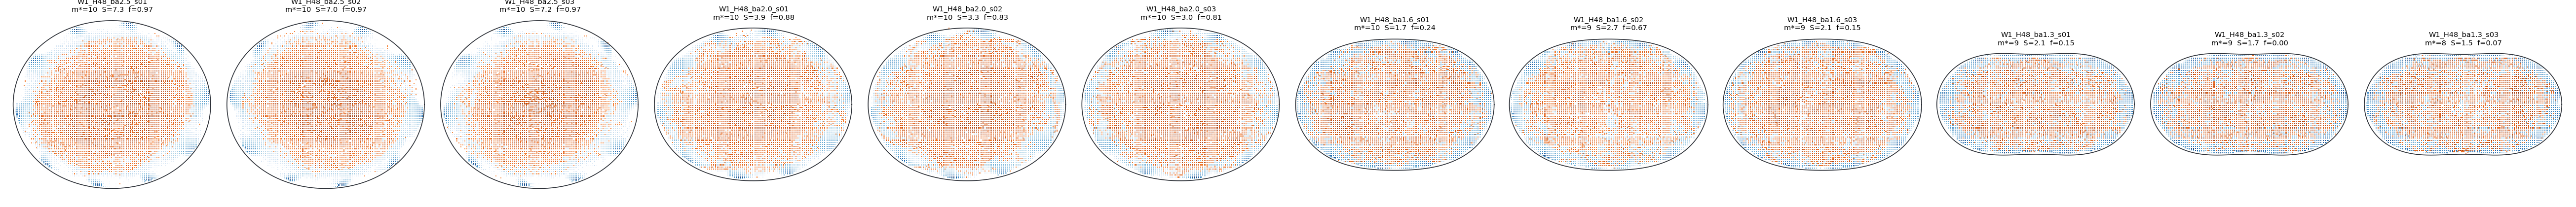
\includegraphics[width=\textwidth]{wf_maps_size.png}\\[4pt]
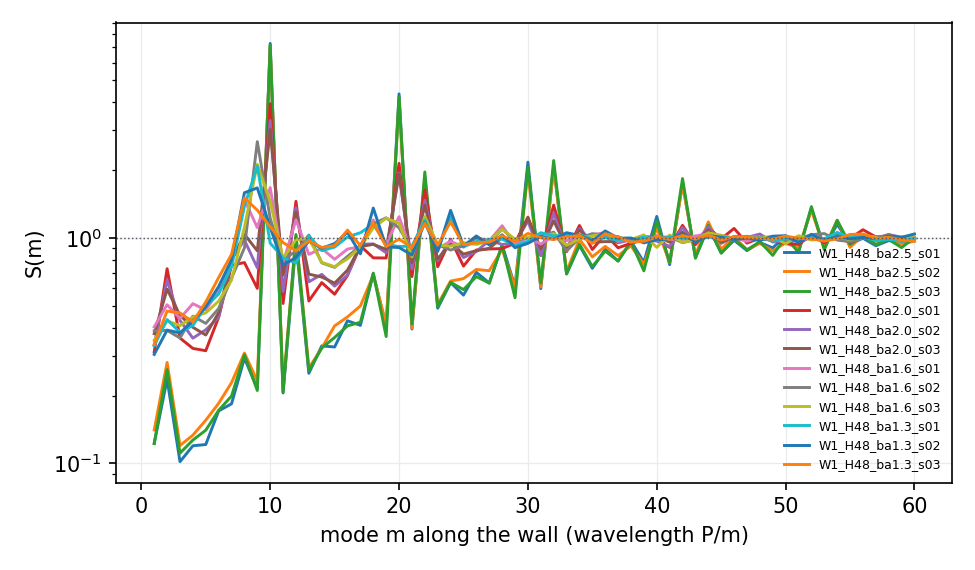
\includegraphics[width=0.7\textwidth]{wf_S_size.png}
\caption{Ovals of half-length $2.16\,\la$ (3 seeds): defect density maps with $m^*$, $S$ and $f_\mathrm{static}$ (top) and the structure
factor $S(m)$ along the wall (bottom).}\label{fig:wfsize}
\end{figure}
\begin{figure}[H]\centering
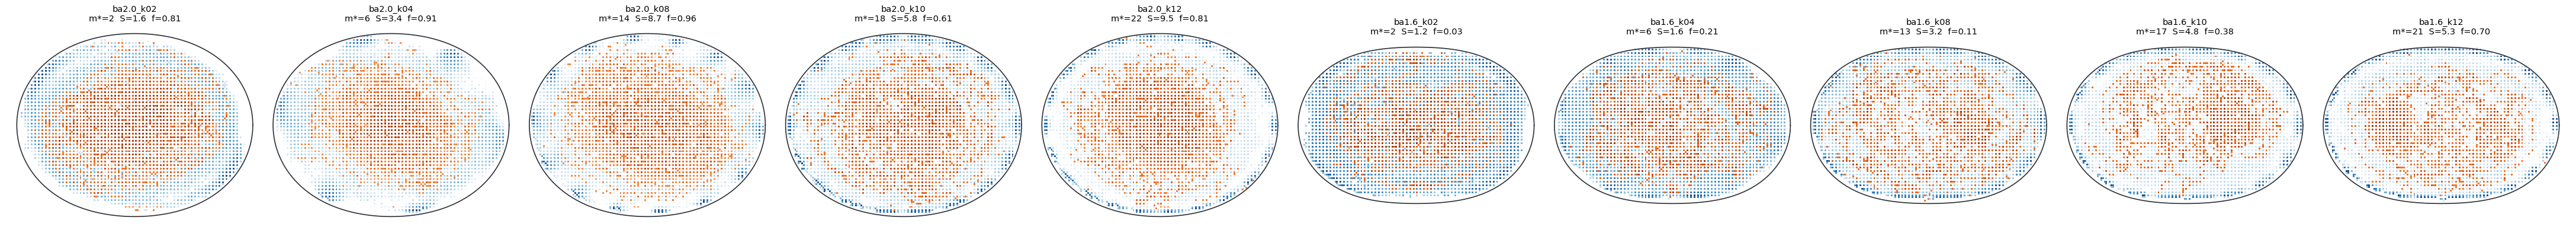
\includegraphics[width=\textwidth]{wf_maps_kscan.png}\\[4pt]
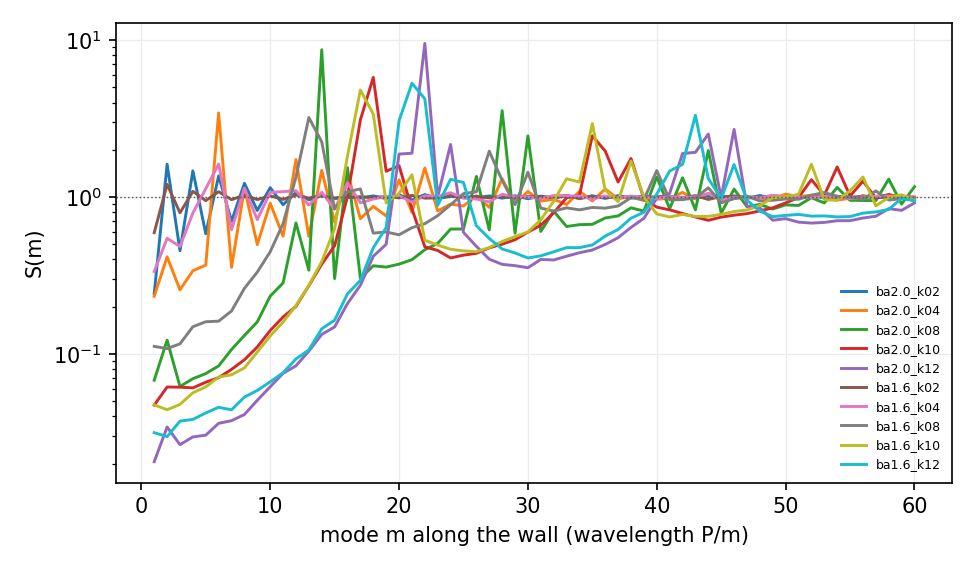
\includegraphics[width=0.7\textwidth]{wf_S_kscan.png}
\caption{$k$ scan (half-length $1.53\,\la$): the wall lattice reappears as $k$ grows.}\label{fig:wfk}
\end{figure}
\begin{figure}[H]\centering
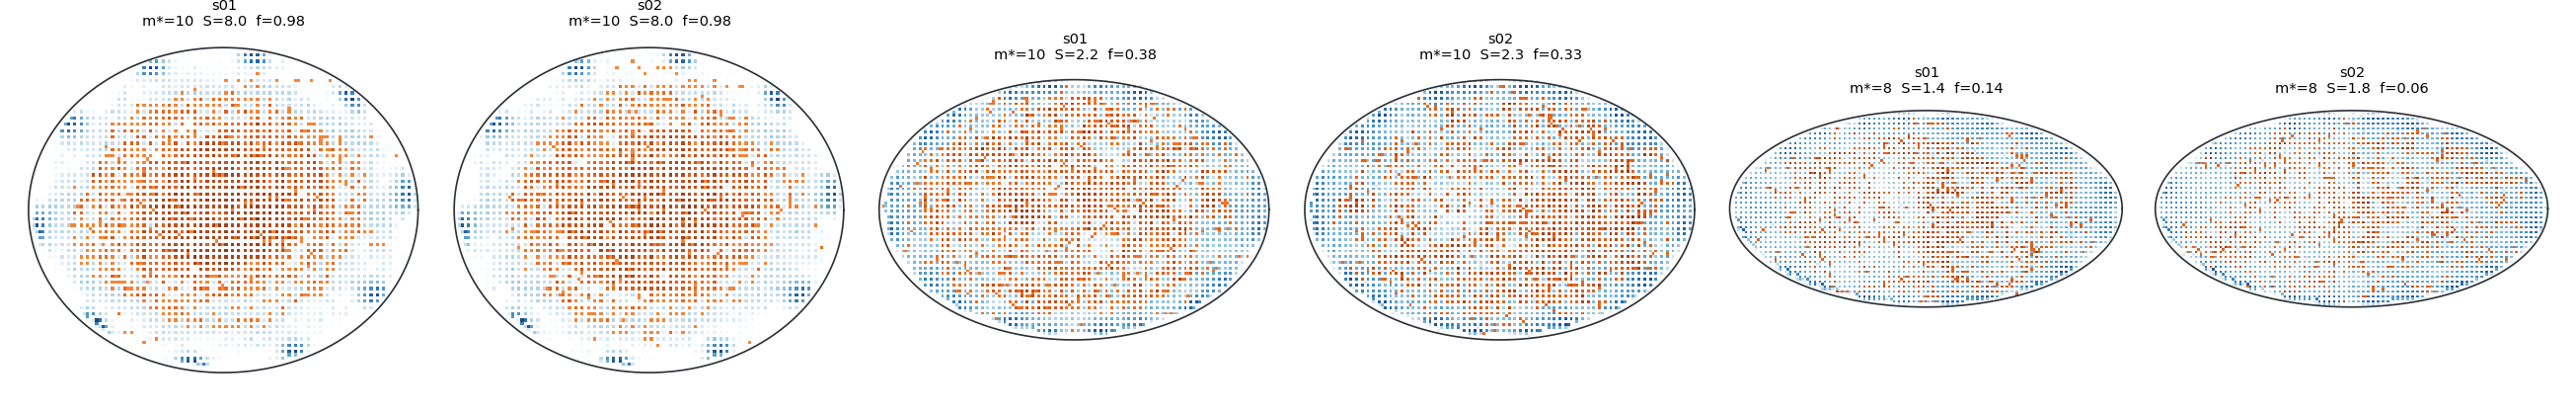
\includegraphics[width=\textwidth]{wf_maps_ellipses.png}\\[4pt]
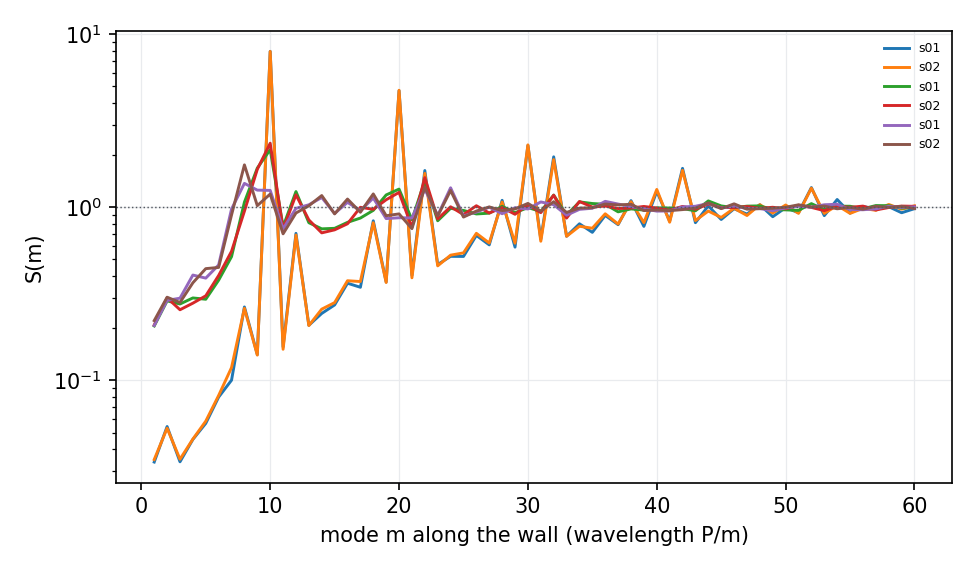
\includegraphics[width=0.7\textwidth]{wf_S_ellipses.png}
\caption{Ellipses: maps and $S(m)$.}\label{fig:wfell}
\end{figure}
\begin{figure}[H]\centering
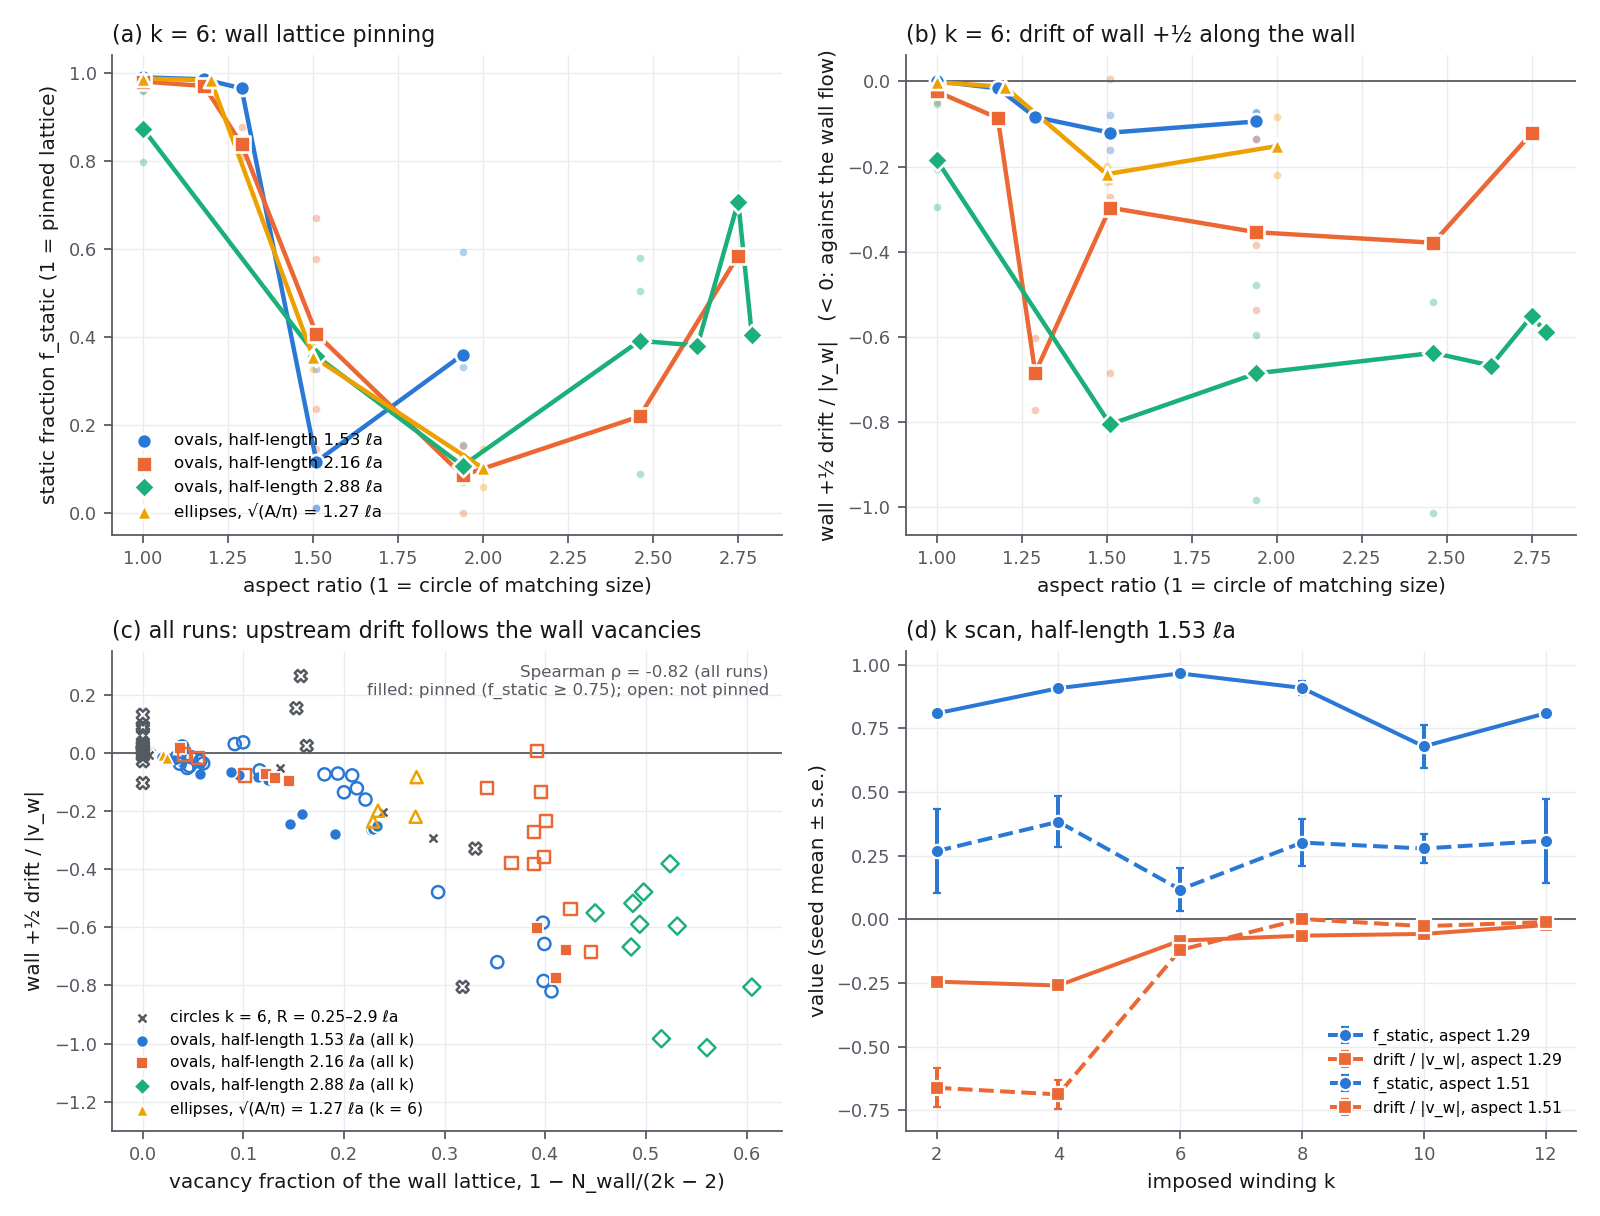
\includegraphics[width=\textwidth]{wall_dynamics.png}
\caption{\textbf{Wall lattice dynamics, ovals and ellipses against circles.} (a) Static fraction against aspect ratio ($k=6$; circles of
matching size at aspect 1, in the colour of the family they match: H34 $\leftrightarrow$ $1.43\,\la$, H48 $\leftrightarrow$ 2.15,
H64 $\leftrightarrow$ 2.87, ellipses $\leftrightarrow$ 1.23). (b) Per-defect drift of wall $+\half$ along the wall divided by the
near-wall flow speed $|v_w|$ (negative = upstream). (c) Drift against the vacancy fraction $1-N_\mathrm{wall}/(2k-2)$, all runs (filled:
pinned lattice, $f_\mathrm{static}\ge0.75$). (d) $k$ scan.}\label{fig:walldyn}
\end{figure}
\begin{itemize}
  \item \textbf{No sliding ordered layer in ovals either.} Where a lattice exists it is pinned (lattice phase speed $\approx0$). Where the
        order is weak ($S/N\lesssim0.4$) the phase of the lattice mode is noise, so the per-defect drift replaces it.
  \item \textbf{Pinning is lost with elongation} ($f_\mathrm{static}$ 0.97 $\to$ 0.1--0.4 from aspect 1.2 to 1.5), at the same aspect
        ratio as the charge split (Sec.~\ref{sec:scharge}); the H48 $b/a=2.0$ oval is the intermediate case: still pinned (0.81--0.88) but
        with only $\approx6$ of 10 sites occupied.
  \item \textbf{The near-wall flow turns with the bulk vortex} (sign agreement 100\% with one strong vortex; 60--90\% in elongated
        cavities, where $|v_w|$ drops from 0.2--0.35 to 0.03--0.07).
  \item \textbf{Wall $+\half$ creep against the wall flow, at a rate set by the vacancies of the lattice, not by its pinning:} Spearman
        $\rho_s=-0.82$ between drift$/|v_w|$ and the vacancy fraction over all runs ($-0.93$ among pinned lattices), against $+0.18$ for
        $f_\mathrm{static}$. Full circles: no drift. The H48 $b/a=2.0$ oval: pinned, 41\% empty, creeps at 69\% of the wall flow.
        Elongated ovals: $-10$ to $-80\%$. Reading: defects hop upstream into empty sites, so the vacancies travel downstream.
  \item \textbf{Crowded walls stop the creep:} in the $k$ scan it vanishes from $k=6$--8 on as the occupancy reaches 0.9--0.97;
        likewise in the pinched oval at $k=12$--20.
  \item Caveats: drift ratios are noisy for tiny circles without a vortex and for single-seed cavities; the drift includes defects
        entering or leaving the wall band. Circle drifts are normalised by the near-wall flow here; the circle sliding speeds in
        Sec.~\ref{sec:clattice} by the interior flow.
\end{itemize}

\subsection{Are the wall defects stationary, and where along the wall do they sit?}\label{sec:stationary}
Two direct tests of the protection of the wall layer (methods: Sec.~\ref{sec:m-tips}): how far a wall $+\half$ travels along the
wall while it stays in the wall band, and how the wall defects are distributed between the tips and the flanks of the ellipses.
\begin{table}[H]\centering\small
\caption{Along-wall travel of wall $+\half$ ($k=6$). For every pair of frames 50 or 500 time units apart in which a track stays within
4 cells of the wall throughout: number of pairs, median along-wall displacement $|\Delta s|$, and fraction with $|\Delta s|$ larger than
half the site spacing $P/(2(2k-2))\approx9$--10 cells (15 cells for the $2.15\,\la$ circle). The detection jitter is $\approx1$ cell.
Seed 1 unless two seeds are given (\texttt{reports/master/data/wall\_travel.txt}).}\label{tab:travel}
\begin{adjustbox}{max width=\textwidth}
\begin{tabular}{lcccccc}\toprule
& \multicolumn{3}{c}{lag 50} & \multicolumn{3}{c}{lag 500}\\
cavity & pairs & median $|\Delta s|$ & $>\frac12$ spacing & pairs & median $|\Delta s|$ & $>\frac12$ spacing\\\midrule
circle $1.43\,\la$ (2 seeds) & 37\,500 & 0.90--0.97 & 0--0.1\% & 23\,000 & 0.93 & 0--0.1\%\\
circle $2.15\,\la$ & 32\,779 & 1.15 & 0 & 9\,324 & 1.15 & 0\\
passive ellipses $\varepsilon=1.5$, 2.0 & 13\,700 & 0.99--1.00 & 0 & 8\,500--9\,300 & 1.05--1.22 & 0\\
ellipse $\varepsilon=1.2$ (2 seeds) & 35\,300 & 0.98--1.00 & 0--0.1\% & 18\,600--19\,500 & 0.97--0.98 & 0\\
oval $b/a=2.5$ (aspect 1.17) & 34\,925 & 0.97 & 0.1\% & 18\,072 & 0.97 & 1.4\%\\
ellipse $\varepsilon=1.5$ (2 seeds) & 18\,000 & 1.47--1.50 & 3.2--3.3\% & 607--923 & 2.0--3.1 & 24--31\%\\
ellipse $\varepsilon=2.0$ (2 seeds) & 16\,200--16\,600 & 1.95--2.00 & 3.1--3.6\% & 149--306 & 2.3--8.4 & 9--34\%\\
oval $b/a=1.6$ & 18\,820 & 1.48 & 3.7\% & 1\,165 & 2.06 & 20\%\\
oval $b/a=1.3$ & 21\,143 & 1.98 & 4.0\% & 1\,715 & 2.05 & 12\%\\\bottomrule
\end{tabular}
\end{adjustbox}
\end{table}
\begin{itemize}
  \item \textbf{Round cavities keep a protected, stationary layer.} In circles, the $\varepsilon=1.2$ ellipse and the $b/a=2.5$ oval the
        wall defects do not move beyond the detection jitter even over 500 time units, exactly as in the passive cavities, and
        30--70\% of the wall-band pairs at lag 50 are still in the band at lag 500 (28\% for the $2.15\,\la$ circle, 52--61\% for the other
        round cavities, 62--68\% passive).
  \item \textbf{In elongated cavities the wall defects wander and leave.} Within 50 time units they move twice as far along the wall
        ($1.5$--2 cells) and 3--4\% shift by more than half a site spacing; after 500 time units only 1--8\% are still in the wall band
        (the fast escape of Sec.~\ref{sec:ssurv}), and 9--34\% of those have shifted by more than half a spacing. The motion is
        individual wandering and hopping, not a sliding lattice (lattice phase speed $\approx0$), with a net upstream drift
        (Fig.~\ref{fig:walldyn}).
\end{itemize}
\begin{table}[H]\centering\small
\caption{Ellipses, $k=6$: spacing of the wall defects at the tips and on the flanks. Per frame, the arclength gaps between neighbouring wall
$+\half$ are assigned to the tips (gap midpoint at $|x|>A/\sqrt2$) or to the flanks; density ratio $=\langle\text{gap}\rangle_\text{flank}/
\langle\text{gap}\rangle_\text{tip}$: 1 for uniform spacing, $\varepsilon$ for the conductor distribution (the one that screens the interior
completely). Theory: passive equilibrium of 12 $+\half$ with uniform winding per arclength (Sec.~\ref{sec:theory}).
(\texttt{reports/master/data/wall\_gaps.txt})}\label{tab:tips}
\begin{adjustbox}{max width=\textwidth}
\begin{tabular}{lcccc}\toprule
ellipse (tip gap / flank gap in cells, density ratio) & passive simulation & active simulation (2 seeds) & passive theory & conductor\\\midrule
$\varepsilon=1.2$ & 15.1 / 14.7, \textbf{0.97} & 19.8 / 17.2, \textbf{0.87} & 14.8 / 14.9, 1.00 & 1.2\\
$\varepsilon=1.5$ & 15.5 / 15.1, \textbf{0.98} & 27.5 / 21.2, \textbf{0.77} & 15.2 / 15.3, 1.01 & 1.5\\
$\varepsilon=2.0$ & 16.3 / 16.1, \textbf{0.98} & 29.7 / 24.6, \textbf{0.83} & 16.1 / 16.1, 1.01 & 2.0\\\bottomrule
\end{tabular}
\end{adjustbox}
\end{table}
\begin{itemize}
  \item \textbf{Passive:} the imposed defects are evenly spaced along the arclength (density ratio 0.97--0.98), as the anchoring imposes and
        as the elastic theory predicts for winding uniform in arclength (1.00--1.01). They do not move towards the screening (conductor)
        distribution, which would need gaps $\varepsilon$ times smaller at the tips.
        \emph{Correction:} an earlier version compared the number of wall defects per unit length at the tips and on the flanks and read
        a tip excess growing with $\varepsilon$; with 12 discrete defects that count is set by how the ring sits (6 of 12 in the tip regions
        in every passive run) and does not measure the spacing.
  \item \textbf{Active:} the gaps at the tips are 15--30\% larger than on the flanks (density ratio 0.77--0.87): activity depletes the tips,
        away from the screening distribution. This holds even for $\varepsilon=1.2$, which keeps its layer, so tip depletion alone does not mean
        loss of the layer.
  \item \textbf{Reading.} The passive layer is uniform, so an ellipse is screened less well than a circle; the theory (Sec.~\ref{sec:theory})
        puts the leftover field in the inner part of the cavity at $\lesssim0.06\,\pi K$ for $\varepsilon=2$, small compared with the energies of
        approach near the wall. In the active ellipses the defects wander, deplete the tips, drift upstream and escape: the flow, not the
        weak unscreened elastic field, drives the loss of the layer. 1--2 seeds per shape; the running shape sweep will repeat both measures
        at all sizes and densities with 3 seeds.
\end{itemize}

%=====================================================================
\section{Flow in ovals: one vortex or two}\label{sec:sflow}
Mean azimuthal velocity about the centroid of each half of the cavity, its persistence, the fraction of frames in which both
halves turn the same way, and reversals (Sec.~\ref{sec:md-lobes}).
\begin{table}[H]\centering\small
\caption{Lobe rotation, $k=6$. $\langle v_\phi\rangle$: time-averaged azimuthal velocity about each half's centroid (L, R);
$|v_\phi|/|v|$: coherence; co-rot: fraction of frames with the same sense; reversals: sign changes; whole: rotation about the cavity
centre. Small ovals: 3 seeds each (one row per seed).}\label{tab:lobes}
\begin{adjustbox}{max width=\textwidth}
\begin{tabular}{lccccccc}\toprule
cavity & $b/a$ & waist & $\langle v_\phi\rangle$ L / R & $|v_\phi|/|v|$ L / R & co-rot & reversals L / R & whole\\\midrule
H34 (small) & 2.5 & 57.9 & $\pm0.42$--0.45 (same sign) & 0.66--0.69 & 1.00 & 0 / 0 & $\pm0.61$--0.64\\
H34 (small) & 2.0 & 52.7 & $\pm0.32$--0.36 (same sign) & 0.55--0.63 & 0.99--1.00 & 0--2 / 0 & $\pm0.50$--0.54\\
H34 (small) & 1.6 & 45.0 & $-0.05$--$+0.09$ & 0.54--0.68 & 0.19--0.31 & 7--18 / 9--16 & $\pm0.09$--0.10\\
H34 (small) & 1.3 & 34.4 & $-0.23$--$+0.22$ & 0.65--0.77 & 0.15--0.48 & 4--13 / 6--13 & $\le0.006$\\
H48 & 1.6 & 63.5 & $+0.32$ / $-0.26$ & 0.67 / 0.54 & 0.15 & 3 / 3 & $+0.05$\\
H48 & 1.3 & 48.6 & $+0.18$ / $-0.17$ & 0.48 / 0.44 & 0.34 & 8 / 5 & $-0.00$\\
H48 & 1.1 & 29.6 & $-0.04$ / $-0.12$ & 0.54 / 0.60 & 0.75 & 7 / 4 & $-0.00$\\
H48 & 1.02 & 13.5 & $+0.19$ / $-0.27$ & 0.64 / 0.72 & 0.14 & 2 / 0 & $-0.01$\\
H64 & 1.6 & 84.7 & $+0.14$ / $-0.32$ & 0.34 / 0.57 & 0.31 & 13 / 4 & $-0.24$\\
H64 & 1.3 & 64.8 & $+0.10$ / $-0.17$ & 0.39 / 0.59 & 0.72 & 11 / 8 & $-0.01$\\
H64 & 1.1 & 39.5 & $-0.23$ / $-0.25$ & 0.49 / 0.54 & 0.88 & 4 / 4 & $-0.03$\\
H64 & 1.01--1.05 & 12.8--28.3 & mixed & 0.63--0.70 & 0.25--0.83 & 1--3 / 0--4 & $\le0.05$\\\bottomrule
\end{tabular}
\end{adjustbox}
\end{table}
\begin{itemize}
  \item \textbf{One vortex for the round shapes, two for the elongated ones, at the same crossover as the charge split.} In the small ovals
        $b/a=2.5$ and 2.0 (aspect 1.17, 1.29) the whole cavity rotates as one vortex in every seed (both halves in the same sense in
        99--100\% of frames, no reversals, whole-cavity rotation 0.5--0.6). At $b/a=1.6$ and 1.3 (aspect $\ge1.5$) the halves rotate
        independently (same sense in only 15--48\% of frames) and reverse 4--18 times per run; the whole-cavity rotation vanishes.
  \item Larger ovals carry two vortices already at $b/a=1.6$. The relative sense of the lobes is not monotonic in the neck width
        (counter-rotating at 1.6, mostly counter at 1.3, mostly co-rotating at 1.1, counter at 1.02; 1 seed each) and reverses
        within runs. Compare Wioland et al.\ (2016), gap-dependent co- and counter-rotation of coupled bacterial vortices (to verify).
  \item The area-mean vorticity of a no-slip region is $\approx0$ (Stokes), so the rotation sense must come from $v_\phi$ about a centre,
        not from the vorticity.
  \item \textbf{Candidate mechanism for the layer loss:} with two vortices the flows meet along the wall (stagnation regions), and the
        near-wall flow there is weak and changes sign (Sec.~\ref{sec:slattice}); a single circular vortex shears the whole wall
        uniformly. Wall defects in elongated cavities lose their pinned sites where the vortices meet. Not yet tested directly.
\end{itemize}
\open{Map where along the wall the vacancies and escapes occur (relative to the vortex stagnation points); measure the near-wall flow and
the tilt along the arclength in ovals. So far the tilt in ovals is known only as a distribution (Fig.~\ref{fig:critsmall}): one sign
in the round ovals, both signs in the elongated ones, as expected for one and two vortices.}

%=====================================================================
\section{Survival of wall defects and docking in ovals and ellipses}\label{sec:ssurv}
Same measures as Sec.~\ref{sec:csurv}; the survival figure (Fig.~\ref{fig:surv}) contains all shapes.
\begin{table}[H]\centering\small
\caption{Wall-visit survival and docking, $k=6$ unless noted (seeds: H34 and H48 3, ellipses 2, lobe oval 3).
Escape rate in $10^{-3}$ per wall defect per time unit (mean $\pm$ s.e.\ over seeds); docking rate per 100 cells of wall per time
unit; $P_\mathrm{dock}$: fraction of bulk $+\half$ episodes that end at the wall. Median times in the bulk before docking (21--76 time units) are in \texttt{reports/master/data/survival\_docking.txt}.}\label{tab:ssurv}
\begin{adjustbox}{max width=\textwidth}
\begin{tabular}{lcccccccc}\toprule
cavity & aspect & visits & wall $+\half$ & escape rate & $S(1000)$ & $t_{1/2}$ & dock rate & $P_\mathrm{dock}$\\\midrule
circle $1.43\,\la$ & 1 & 73 & 10.0 & $0.34\pm0.07$ & 0.50 & 1000 & 0.0015 & 0.10\\
circle $2.15\,\la$ & 1 & 98 & 9.9 & $0.41\pm0.16$ & 0.51 & 1044 & 0.0014 & 0.04\\
H34 $b/a=2.5$ & 1.18 & 145 & 9.9 & $0.65\pm0.07$ & 0.39 & 666 & 0.0030 & 0.19\\
H34 $b/a=2.0$ & 1.29 & 668 & 9.1 & $3.2\pm0.2$ & 0.05 & 100 & 0.015 & 0.54\\
H34 $b/a=1.6$ & 1.51 & 1039 & 8.1 & $6.0\pm0.1$ & 0.009 & 84 & 0.024 & 0.67\\
H34 $b/a=1.3$ & 1.94 & 998 & 8.2 & $5.7\pm0.1$ & 0.007 & 98 & 0.024 & 0.73\\
H48 $b/a=2.5$ & 1.18 & 577 & 9.2 & $2.7\pm0.1$ & 0.07 & 102 & 0.009 & 0.27\\
H48 $b/a=2.0$ & 1.29 & 1433 & 6.2 & $10.8\pm0.5$ & 0.001 & 52 & 0.022 & 0.46\\
H48 $b/a=1.6$ & 1.51 & 1350 & 6.2 & $10.6\pm0.5$ & 0 & 62 & 0.022 & 0.47\\
H48 $b/a=1.3$ & 1.94 & 1372 & 6.2 & $10.5\pm0.5$ & 0 & 62 & 0.023 & 0.53\\
ellipse $\varepsilon=1.2$ & 1.2 & 120 & 9.9 & $0.83\pm0.03$ & 0.33 & 368 & 0.0042 & 0.30\\
ellipse $\varepsilon=1.5$ & 1.5 & 731 & 7.9 & $6.4\pm0.05$ & 0.009 & 90 & 0.025 & 0.67\\
ellipse $\varepsilon=2.0$ & 2.0 & 788 & 7.4 & $7.2\pm0.1$ & 0.003 & 72 & 0.025 & 0.72\\
lobe oval ($k=3$) & 1.38 & 530 & 2.8 & $8.3\pm0.3$ & 0.002 & 70 & 0.013 & 0.61\\\bottomrule
\end{tabular}
\end{adjustbox}
\end{table}
\begin{figure}[H]\centering
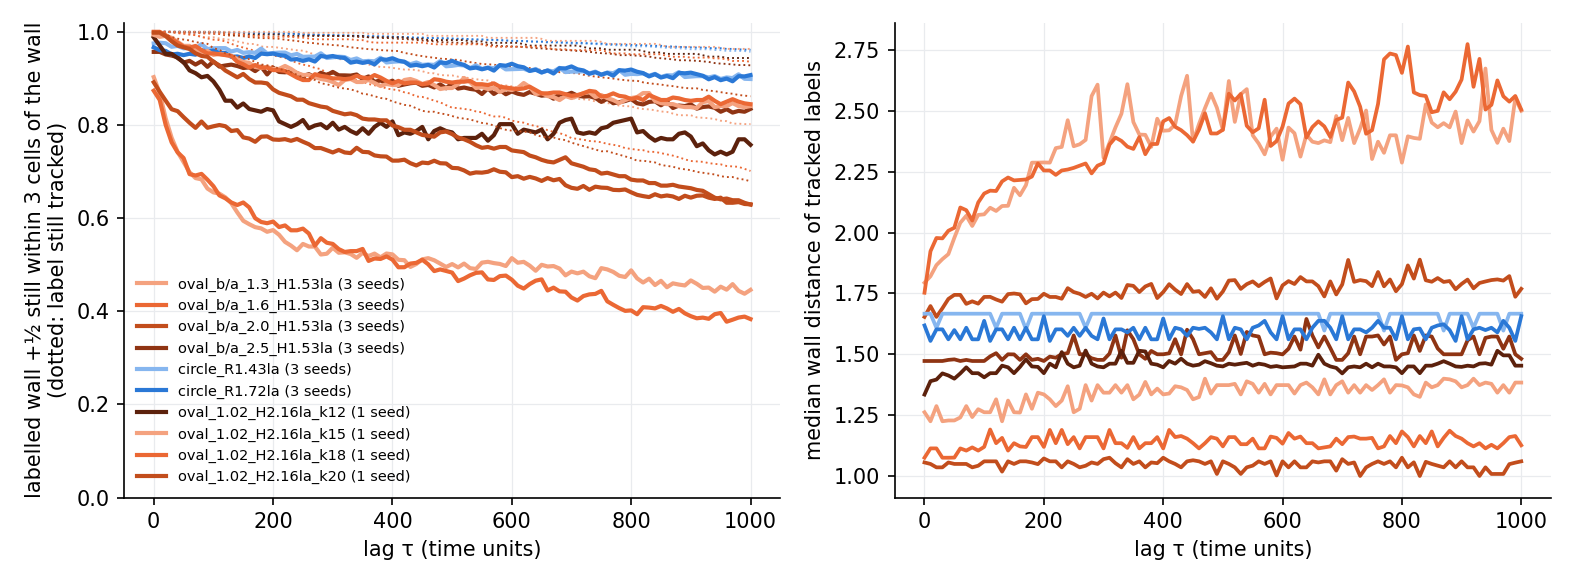
\includegraphics[width=\textwidth]{labels_small_ovals.png}
\caption{Label survival: small ovals ($b/a=2.5\to1.3$, 3 seeds, orange light to dark), circles of $1.43$ and $1.72\,\la$ (blue, 3 seeds) and the pinched oval at $k=12$--20 (1 seed). Left: fraction of labelled wall defects within 3 cells of the wall (dotted: label still tracked); right: median wall distance of tracked labels.}\label{fig:labsmall}
\end{figure}
\begin{figure}[H]\centering
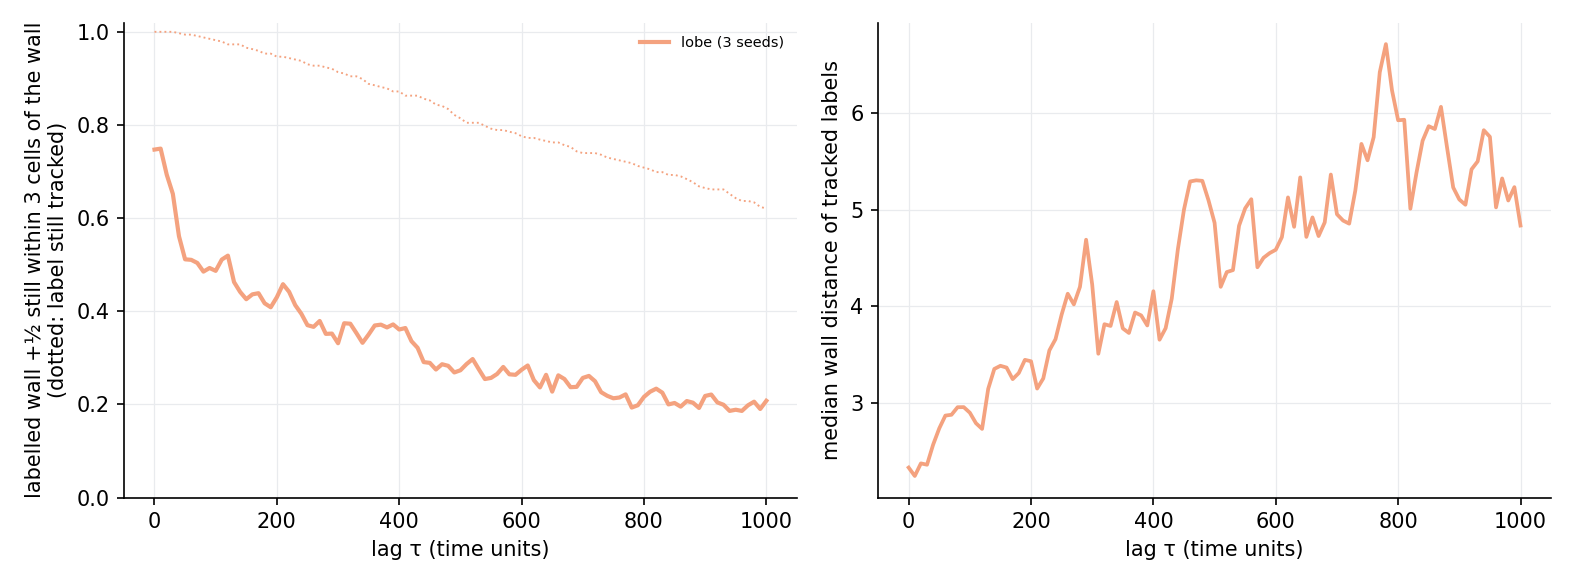
\includegraphics[width=0.85\textwidth]{labels_lobe_oval.png}
\caption{Label survival in the lobe-shaped oval ($k=3$, seed 1 shown; seeds 2--3: 16--28\% at the wall after 1000).}\label{fig:lablobe}
\end{figure}
\begin{itemize}
  \item \textbf{Wall defects in elongated cavities do not stay:} escape rates $6$--$11\times10^{-3}$, 17--30$\times$ the clean circles; half
        of the wall visits end within 50--100 time units, and essentially none last 1000 (circles: half last longer than 1000). Label
        survival agrees: in the small ovals 37--50\% of labels at the wall after 1000 for $b/a\le1.6$ (circle 87--94\%), in the larger ovals
        6--39\%.
  \item \textbf{Docking becomes the norm:} 46--73\% of bulk $+\half$ excursions end at the wall in elongated cavities, against 4--10\% in
        clean circles. The layer and the bulk exchange continuously, so ``layer'' and ``bulk'' stop being separate populations.
  \item \textbf{The crossover is the same as for the charge, pinning and the vortex:} round shapes ($b/a=2.5$, $\varepsilon=1.2$) stay close
        to circles (escape 0.65--0.83$\times10^{-3}$ at half-length $1.53\,\la$), elongated ones (aspect $\ge1.5$) are fully exchanging;
        $b/a=2.0$ (aspect 1.29) is intermediate.
  \item \textbf{Size matters on top of shape:} at half-length $2.16\,\la$ even $b/a=2.5$ escapes 4$\times$ faster than at $1.53\,\la$, and the
        elongated shapes saturate at $\approx10^{-2}$ with only 6 of 10 sites occupied; at this size circles are still clean.
  \item At most 10\% of wall visits end in annihilation: the layer empties by undocking, not by annihilation of wall defects.
\end{itemize}

%=====================================================================
\section{Negative winding in ellipses: is the shape effect elastic or active?}\label{sec:smirror}
With positive winding the wall layer is made of self-propelled $+\half$, so its loss in elongated cavities could come from either of two
mechanisms: (1) \emph{lost shielding} (elastic and sign-symmetric: an evenly spaced layer cannot screen a non-circular interior,
Sec.~\ref{sec:theory}), or (2) \emph{motility and flow} (the two-vortex flow carries the motile wall $+\half$ off the wall). With negative winding
the wall carries $-\half$, which are not self-propelled. Mechanism (1) predicts a disrupted $-\half$ layer, more annihilation of bulk $+\half$ at the
wall and a smaller positive bulk in ellipses; mechanism (2) predicts that the $-\half$ layer survives elongation.

\paragraph{Runs.} \texttt{runs/cassini/P6\_mirror\_shapes/}: circle and ellipses $\varepsilon=1.2$, 1.5, 2.0 of area 2500 ($\sqrt{A/\pi}=1.27\,\la$,
arclength anchoring, eMode 2) at $k=-6$ ($\rho\approx0.06$--0.07) and $k=-12$ ($\rho\approx0.12$--0.14), 2 seeds, 10k + 100k steps, outputs as the
positive-winding ellipses; passive references (circle and $\varepsilon=2.0$ at $k=-6$, $-12$). \textbf{Validation:} the passive references carry
exactly $2|k|$ $-\half$ (12.00 and 23.99 per frame) and no $+\half$, the first check of eMode 2 with negative winding.
Analyses: \texttt{wall\_sign\_analysis.py} (sign-aware wall lattice, travel, survival, charge; \texttt{data/mirror\_shapes\_wall.tsv}) and
\texttt{shielding\_test.py} (\texttt{data/shielding\_mirror\_*.tsv}).

\begin{figure}[H]\centering
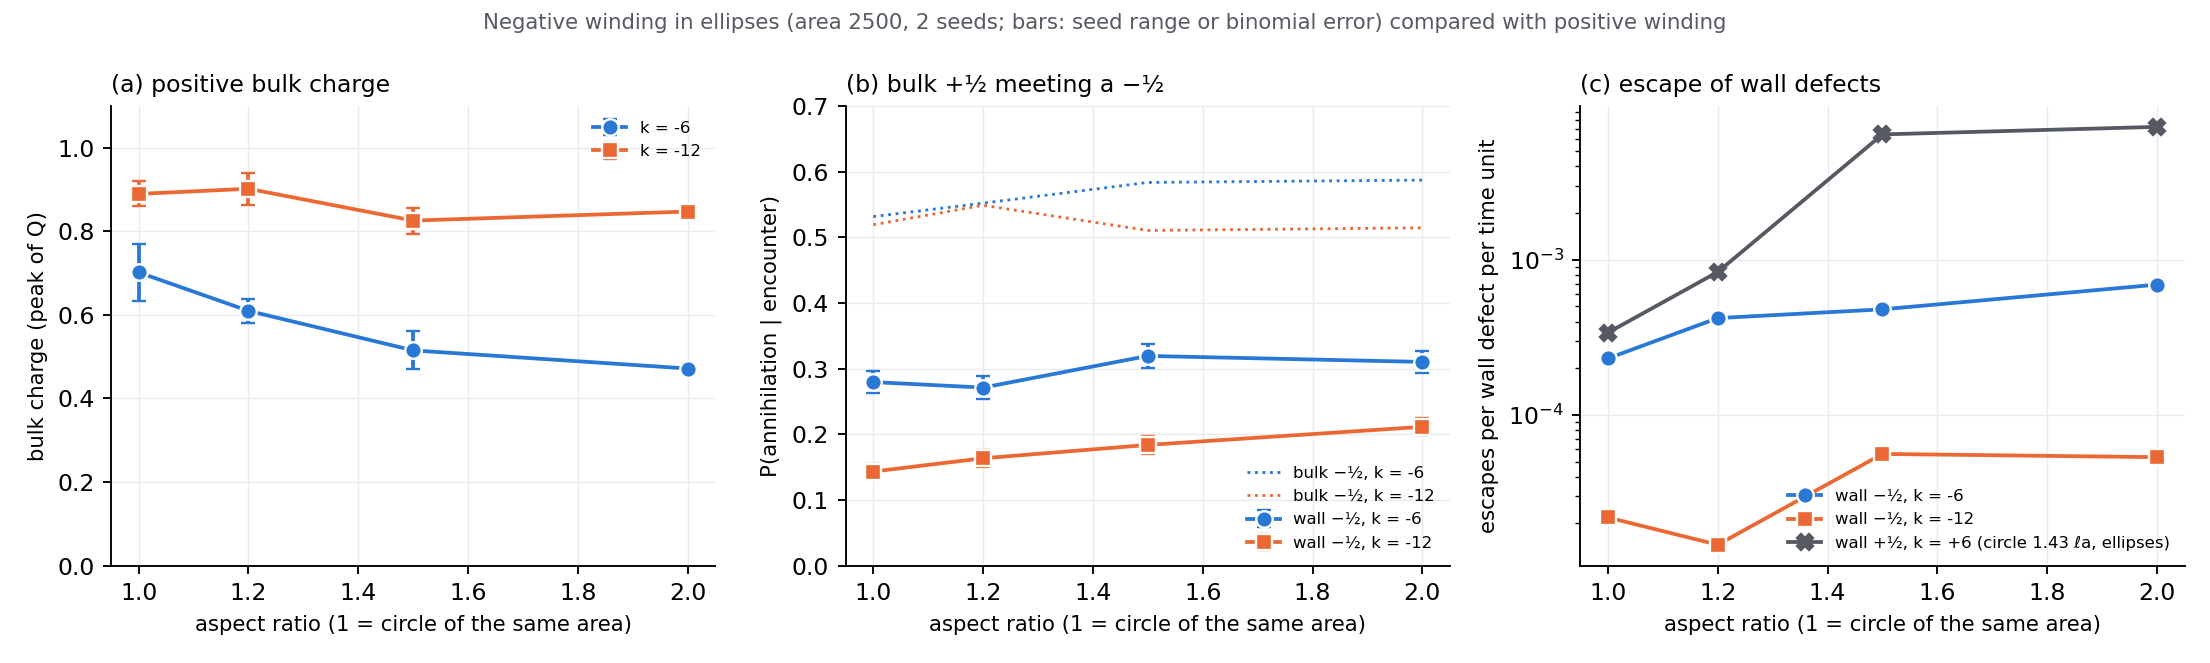
\includegraphics[width=\textwidth]{mirror_ellipses.png}
\caption{\textbf{Negative winding in ellipses.} (a) Positive bulk charge (peak of $Q$) against aspect ratio, $k=-6$ and $-12$. (b) Probability that an
encounter of a bulk $+\half$ with a $-\half$ ends in annihilation: wall targets (solid) and bulk targets (dotted). (c) Escape rate of wall defects:
$-\half$ (negative winding) and, for comparison, $+\half$ in positive-winding ellipses of the same area and the circle of $1.43\,\la$ (grey). 2 seeds;
bars: seed range in (a), binomial error in (b).}\label{fig:smirror}
\end{figure}
\begin{table}[H]\centering\small
\caption{Negative winding in ellipses (2 seeds; ranges over seeds). Occupancy: wall $-\half$ per frame over $2|k|+2$; pinning: static fraction of
the wall lattice at $m=2|k|+2$; escape: per wall defect per time unit; annihilation: probability that an encounter of a bulk $+\half$ with a wall
$-\half$ ends in annihilation (with a bulk $-\half$ in brackets).}\label{tab:smirror}
\begin{adjustbox}{max width=\textwidth}
\begin{tabular}{llcccc}\toprule
& & circle & $\varepsilon=1.2$ & $\varepsilon=1.5$ & $\varepsilon=2.0$\\\midrule
$k=-6$ & bulk charge & 0.63--0.77 & 0.58--0.64 & 0.47--0.56 & 0.46--0.48\\
& wall occupancy & 0.95--0.97 & 0.94--0.95 & 0.93--0.94 & 0.93\\
& pinning $f$ & 0.56--0.72 & 0.65--0.77 & 0.29--0.43 & 0.22--0.32\\
& escape ($10^{-4}$) & 2.3 & 4.1--4.3 & 4.8 & 6.4--7.4\\
& annihilation at the wall (bulk) & 0.28 (0.53) & 0.27 (0.55) & 0.32 (0.58) & 0.31 (0.59)\\\midrule
$k=-12$ & bulk charge & 0.86--0.92 & 0.86--0.94 & 0.79--0.86 & 0.84--0.86\\
& wall occupancy & 0.99 & 0.99 & 0.99 & 0.99\\
& pinning $f$ & 0.59--0.85 & 0.68--0.69 & 0.62--0.69 & 0.55--0.60\\
& escape ($10^{-4}$) & 0.2 & 0.1--0.2 & 0.5--0.6 & 0.5--0.6\\
& annihilation at the wall (bulk) & 0.14 (0.52) & 0.16 (0.55) & 0.18 (0.51) & 0.21 (0.51)\\\bottomrule
\end{tabular}
\end{adjustbox}
\end{table}
\begin{itemize}
  \item \textbf{The $-\half$ wall layer survives elongation.} Occupancy stays at 0.93--0.99 and the wall $-\half$ rarely leave: the escape rate rises
        $\approx3\times$ from the circle to $\varepsilon=2$, against $\approx20\times$ for the wall $+\half$ with positive winding (Fig.~\ref{fig:smirror}c).
        The layer loses its lattice order along the wall at $k=-6$ (pinning 0.56--0.77 $\to$ 0.22--0.32), but its defects stay at the wall.
  \item \textbf{Shielding weakens a little, as the elastic theory predicts.} A bulk $+\half$ meeting a wall $-\half$ annihilates somewhat more often in
        elongated cavities (0.28 $\to$ 0.31 at $k=-6$, 0.14 $\to$ 0.21 at $k=-12$), still far less often than with a bulk $-\half$ (0.51--0.59). At $k=-6$
        the positive bulk shrinks from $\approx0.7$ to $\approx0.47$; at $k=-12$ (crowded wall) there is no shape effect.
  \item \textbf{Conclusion.} Both mechanisms act, with very different strengths. Geometry weakens the elastic shielding for both signs, modestly
        (Sec.~\ref{sec:theory}); the dramatic loss of the layer with positive winding needs self-propelled wall defects, which the two-vortex flow carries
        off the wall. The shape effect of Part~III is therefore mainly an active effect enabled by geometry.
  \item The wall $-\half$ also travel along the wall in the circle (median 11--12 cells in 500 time units, 65\% beyond half a site spacing at $k=-6$),
        unlike wall $+\half$ in circles: the mirror wall layer creeps even without elongation, consistent with its lower pinning in the circle sweep
        (Sec.~\ref{sec:clattice}).
\end{itemize}
\open{Two seeds and one size; ovals with negative winding and a third seed would make this a main-text result (the office machine is free).}


\part{Synthesis}
% Where the theory stands (written 2026-10-08, after the head/tail correction)
\section{Where the theory stands (2026-10-08)}\label{sec:status}
\paragraph{The sign issue in one paragraph.} The defect angle in \texttt{defects.dat} is the direction of $\nabla\!\cdot Q$, which for a $+\half$ points
to its \emph{tail} (the splay side). Verified three ways: the formula in the code, the director field around bulk $+\half$ (director along the axis on the
recorded side, $|\mathbf n\cdot\hat e|=0.92$--0.95, across it on the other, 0.20), and the motion of bulk $+\half$ (against the recorded angle, 66--72\% of steps,
$\approx60\sigma$). Head, self-propulsion and active force point along $-\hat e$. Everything that only uses positions, charges or relative angles is
unaffected (distributions, charge, survival, depth law, shielding, fluctuations, the tilt--position lock); everything that turned a $+\half$ into a force
had the wrong sign (the point-force Stokes models, the feedback modes and stage 2).

\paragraph{What holds (equilibrium and elasticity).}
\begin{itemize}
  \item Electrostatics with same-sign images: exact shielding in circles, the depth law (0.984$\times$ prediction + 0.61 cells, $r=0.996$), the approach barrier,
        the weak leftover field in ellipses (Sec.~\ref{sec:theory}).
  \item Fluctuations of the passive wall lattice: along the wall, the exact potential with the measured bend constant $K_3=23\,k_BT$ (plus the detector's cell
        rounding) reproduces the rms within 2--4\%; across the wall a 0.15--0.5 cell excess remains, not explained by fluid noise (random walks); mobility
        $\mu\approx0.02$ (Sec.~\ref{sec:fluct}).
  \item Tilt and position are one variable: for a wall $+\half$, tail angle $-$ normal $=(2k-2)\phi+$const (lock 0.99 in $\approx$150\,000 active frames). The $2k-2$
        sites are where the tails point straight at the wall (heads into the bulk).
  \item Splay $\neq$ bend ($K_1\approx1.8K_3$) pins the active lattice at exactly those sites (barrier 80--110\,$k_BT$ at $k=6$; predicted collective rms 0.5 cells,
        measured 0.3). The \emph{passive} registry is not pinned: runs started from different initial directors settle at different registries and only creep; the
        shared registry of the production runs came from their common initial condition (B.~Loewe's spontaneous-symmetry-breaking hypothesis, confirmed).
        The \emph{active} registry is pinned: eight runs from six different initial directors all sit at the predicted site (after removing the tilt with the
        lock, $D=0.03\pm0.07$, resultant length 1.00); only the sense of rotation is chosen spontaneously.
\end{itemize}

\paragraph{Why the sites are fixed although the cavity is round (symmetry argument).}
\begin{itemize}
  \item \textbf{The winding breaks rotational symmetry to a discrete one.} The code imposes the wall director at lab angle $\theta=k\phi$ (\texttt{lc.c}, $O=0$),
        i.e.\ at $(k-1)\phi$ from the wall normal: homeotropic where $(k-1)\phi\equiv0$ (mod $\pi$), tangential halfway between. A rotation of the cavity by
        $\beta$ turns the pattern into $k\phi-(k-1)\beta$, the same pattern only if $(k-1)\beta\equiv0$ (mod $\pi$): the boundary has a $(2k-2)$-fold symmetry,
        with homeotropic points at $\phi_n=2\pi n/(2k-2)$. Only $k=1$ is fully rotationally symmetric.
  \item \textbf{The active sites are the homeotropic points.} The measured registry (phase 0) puts the $2k-2$ wall $+\half$ at $\phi_n$ with their tails
        (the splay side, where the director is radial) pointing straight at the wall: the radial side of the comet sits where the anchoring is radial. With a
        tilt $\tau$ the lattice is displaced from these points by $\tau/(2k-2)$, in the direction set by the sense of rotation.
  \item \textbf{One-constant elasticity hides this by an extra symmetry.} With a single Frank constant a uniform rotation of the director, independent of space,
        costs nothing; rotating the defects by $\beta$ and adding $(k-1)\beta$ to the director restores the boundary condition at no cost, hence the free sliding mode
        of Sec.~\ref{sec:fluct}. Splay $\neq$ bend breaks this internal symmetry (a director rotated relative to space changes the splay--bend mix) and turns the
        homeotropic points into energy minima.
  \item \textbf{Why the passive ring of $2k$ cannot be untilted.} By the tilt--position lock, a wall $+\half$ at $\phi_j$ has tilt (tail angle minus normal)
        $\tau_j=2\psi_\mathrm{rel}(\phi_j)=2(k-1)\phi_j+\text{const}$ (mod $2\pi$): its tail points at the wall only on a homeotropic point. All tilts vanish only if
        every defect sits on one of the $2k-2$ homeotropic points, impossible for $2k$ defects. For $N$ evenly spaced defects consecutive tilts differ by
        $2(k-1)\cdot2\pi/N$ (mod $2\pi$), zero only if $N$ divides $2(k-1)$; for $N=2k$ the step is $-2\pi/k$, so the tilts wind twice ($-4\pi$) around the ring.
        Measured ($k=6$): $+41^\circ,-20^\circ,-91^\circ,\dots$, steps of $-60^\circ=-2\pi/6$ (Sec.~\ref{sec:fluct}). The passive ring is therefore frustrated:
        most of its defects are tilted whatever the registry, which is why the registry energy averages out (incommensurate, $<1\,k_BT$).
        \emph{Interpretation:} the active state ejects exactly two $+\half$ into the bulk; the remaining $2k-2$ are the largest commensurate ring, which can
        sit untilted on the homeotropic points, so the $+1$ bulk also relieves the tilt frustration of the wall.
  \item \textbf{Commensurability decides how strongly.} The active lattice ($2k-2$ defects) matches the $(2k-2)$-fold pattern: barrier 80--110\,$k_BT$ ($k=6$),
        pinned at the predicted site from every initial condition, only the sense of rotation chosen spontaneously. The passive lattice ($2k$ defects) is
        incommensurate: the lowest harmonics cancel, the barrier is $<1\,k_BT$, and its registry is frozen in from the initial condition and only creeps.
  \item \textbf{Tested:} with a sine-modulated winding $k\phi+A\sin(m\phi)$ (branch \texttt{anchmod}) the active sites follow the unevenly spaced homeotropic points
        (0.21--0.27 cells, any initial director). The passive registry stays free: a modulation with $m$ not a multiple of $2k$ does not couple to an evenly spaced
        $2k$ ring at first order (Sec.~\ref{sec:sitecurv}).
\end{itemize}

\paragraph{What changed (hydrodynamics).}
\begin{itemize}
  \item \textbf{The wall layer does not drive the circulation; it brakes it.} Wall $+\half$ lean with their tails downstream, i.e.\ their heads point into the bulk and
        upstream; their active forces oppose the flow (Sec.~\ref{sec:hydro}, correction box). Withdrawn: ``the wall layer explains 70\% of the flow'', the force
        estimates $f/\eta$ per wall defect, ``the wall layer sustains the circulation'', and the reading of stage 2 as the layer selecting one vortex.
  \item \textbf{The bulk active stress drives the flow, including the two vortices of elongated ellipses.} Stokes flow of the full measured active force
        $-\nabla\!\cdot Q$ (no defect idealisation): one positive coefficient explains 48--72\% of the measured flow; the bulk part alone 47--73\%; the wall band
        opposes the circulation; the bulk reproduces the two-vortex part in ellipses (correlation 0.87--0.91) (Sec.~\ref{sec:dirstokes}).
  \item \textbf{Point-defect hydrodynamics is not enough.} Bulk $+\half$ as point forces explain only 6--21\%; a particle Langevin model with Stokeslets and log
        elasticity neither keeps $2k-2$ defects at the wall nor makes a circulation (Sec.~\ref{sec:defectmodel}).
\end{itemize}

\paragraph{What is new (the layer as an effective boundary).}
\begin{itemize}
  \item Seen from the bulk, the layer converts the $k$-fold patterned anchoring into an effectively \emph{planar} winding-1 boundary (exact, one-constant), smooth
        from $\approx0.34\ell$ from the wall. A tilt $\tau$ makes it a spiral, $c=90^\circ+\tau/2$, whose extensile stress drives the same circulation that tilts the
        layer (Sec.~\ref{sec:effbc}).
  \item This closes a feedback loop through the elastic field, not through forces at the wall. Its linear stability, with calibrated parameters and one assumed
        core size, gives an onset of tilt and circulation at $R/\ell_a\approx0.4$--0.6, where it is measured (Sec.~\ref{sec:effstab}); the predicted $k$-ordering is
        untested.
  \item Spacing does not give an independent criterion for the $+1$ bulk within the sweep: its existence is set by size ($R/\ell_a\ge0.76$, 99\%); $k=2$
        ($N=2$, smoothing depth $\approx R$) is predicted to be anomalous (one data point agrees).
\end{itemize}

\paragraph{Particle model with the spiral flow.} Given the observed structure (layer of $2k-2$ held at the wall, bulk pair kept inside), adding the
spiral flow to the defect Langevin model produces a circulation of the measured size and a tilt that follows it, above $R/\ell_a\approx0.7$ ($k=6$) and
later for $k=4$; without it, nothing. The model still cannot produce the structure itself (Sec.~\ref{sec:effstab}).

\paragraph{The size of the tilt.} To first order, splay $\neq$ bend only resists the tilt (exactly $\propto\cos\tau$). Beyond first order it adds a
$\cos2\tau$ term of the right sign ($+5\,k_BT$ at $k=6$), which makes the onset supercritical with a locked finite tilt; in the particle model this
locks the tilt at $\approx35^\circ$ with the computed size and at $63^\circ$ with a 3--4$\times$ larger term (Sec.~\ref{sec:effstab}).

\paragraph{Flow alignment.} Present in MPCD ($\lambda=2$, Leslie angle $30^\circ$), absent from the models. \emph{Corrected 2026-10-09:} the director at the wall defects' depth is rotated by 26--33$^\circ$
(Sec.~\ref{sec:tiltangle}; the earlier 4--5$^\circ$ estimate was wrong); it but erases the elastic spiral in the bulk (measured $74$--$87^\circ$ against the elastic $122^\circ$); the azimuthal active drive is confined to a ring
just inside the layer ($r/R\approx0.6$--0.9), braked in the wall band (Sec.~\ref{sec:effstab}).

\paragraph{Wall defects are not advected.} Measured: the wall $+\half$ do not move with the fluid at their depth (advection coefficient 0.002--0.004 against
a fluid speed of 0.13--0.16): the tilted layer sits at a static shifted registry. A particle model that advects them with the fluid slides instead of locking, even
with the measured drive (Sec.~\ref{sec:effstab}); the defect kinematics at an anchored wall is the next ingredient.

\paragraph{Site arrangement and curvature.} Moving the active sites with a modulated winding keeps them on the predicted homeotropic points (0.21--0.27 cells,
independent of the initial director) with the tilt unchanged; the passive ring is not pinned by a low-$m$ modulation (it couples only through $\sum e^{im\phi_j}=0$). In ellipses the layer is $\approx14\times$ leakier at $\varepsilon\ge1.5$ in one- and two-vortex intervals alike, with escapes at
the tips: the second vortex is not the immediate cause. A circle sweep with uneven sites (up to $A=3$) leaves every property of the layer unchanged: the site arrangement
does not destabilise it, so the ellipse instability comes from the curvature or the elongated flow (Sec.~\ref{sec:sitecurv}).

\paragraph{Imposed vortex.} With an imposed swirl the active layer behaves as a stick--slip system: pinned until the flow at its depth reverses, then a jump
of the size predicted by the lock. A passive layer under imposed flow also tilts to $\approx\pm60^\circ$ and slides with it. In the cavities the tilt is an active effect (the flow is active), but
its angle is set by the layer's response to flow: it grows with the flow-alignment parameter ($\approx32^\circ$ at $\lambda=0.5$, 60$^\circ$ at 1.2--2, 79$^\circ$ at 4),
not by the simple $2\theta_L$ rule (Sec.~\ref{sec:swirl}).

\paragraph{Half-integer windings.} For $k\ge2.5$ the odd layers (3, 5, 9 wall $+\half$) are pinned on the odd set of homeotropic points with the same lock,
tilt and single vortex as integer $k$; at $k=1.5$ (one site) no layer forms and the flow is weak and erratic, as the effective-boundary picture requires at least two sites;
$k=0.5$ gives a single bulk $+\half$ with a strong vortex (Sec.~\ref{sec:halfk}).

\paragraph{Why the active wall holds $2k-2$: flow-induced ejection.} (B.~Loewe's mechanism.) Flow aligns the wall defects to a common tilt; a $2k$ ring cannot take a
common tilt (its tilts must wind), which costs 375--475\,$k_BT$ at $k=6$ (200--510 for $k=4$--8), about twice the 180--200\,$k_BT$ (155--200) of ejecting two defects; the ejected $2k-2$ ring tilts by a registry shift
almost for free. Directly confirmed: \emph{passive} cavities under an imposed swirl eject two defects (12$\to$10 at the wall, bulk $+1$) for $\lambda=2$, 4, partly at
$\lambda=1.2$, never for tumbling $\lambda=0.5$. Activity enters by providing the flow (Sec.~\ref{sec:ejection}).

\paragraph{Ejection threshold and negative layer.} Passive ejection needs a flow strong enough to impose a common tilt (constant swirl: none up to 0.003, both
seeds at 0.01, tilt coherence 0.2--0.5 $\to$ 0.9). The mirror prediction for $-k$ (the wall gains two $-\half$) is favoured energetically but did not happen in passive runs:
it needs pair creation, rare without activity (Sec.~\ref{sec:ejection2}).

\paragraph{Shapes.} A single transition at aspect 1.25--1.37, scale free and the same for ellipses and ovals: coherence, circulation and the single vortex collapse together,
and the layer then loses defects in proportion to the size. Coherent flow imposed on a \emph{passive} ellipse gives the circle structure. In \emph{active} ellipses the imposed vortex
did not repair the layer, but it also never made the flow circle-like coherent, so activity disrupting the coherence remains a viable cause; stronger forcing is being tested
(Sec.~\ref{sec:shapesweep}).

\paragraph{Open, in order.} (1) Circulation of small high-$k$ cavities to
test the predicted $k$-ordering of the onset. (2) Effective-boundary picture in ellipses: does the bulk active stress of a spiral boundary of an ellipse split
into two vortices, and at which $\varepsilon$? (3) Rewrite of the hydrodynamics subsection around the director-field model (the old text is kept under the
correction box for traceability). (4) What holds the $+1$ in the bulk and the layer at the wall in the active state (the particle model needs it as input). 

%=====================================================================
\section{Elastic theory of the wall layer: shielding}\label{sec:theory}
B.~Loewe's picture: defects of equal charge repel, opposite charges attract, the strongly anchored wall repels every defect, and an evenly
distributed wall layer shields the bulk from its charge. Here it is made quantitative for the passive (elastic) part of the problem.
Scripts: \texttt{reports/master/theory/shielding\_disk.wl} (Mathematica; results in \texttt{shielding\_disk\_results.txt}) and
\texttt{shielding\_ellipse.wl} (conformal map; \texttt{shielding\_ellipse\_results.txt}).

\subsection{Model}
One-constant Frank elasticity, director angle $\theta$, defects of charge $q_i$ at $z_i$. Use the field $\psi$ conjugate to $\theta$
($\nabla\psi=\hat z\times\nabla\theta$), for which defects are point sources, $\nabla^2\psi=2\pi\sum_iq_i\delta(z-z_i)$. Strong anchoring fixes
$\theta$ on the wall, so $\partial_s\theta$ is prescribed: a \emph{Neumann} condition for $\psi$, with flux density equal to the imposed winding per
length ($2\pi k/P$ for winding uniform in arclength). In a disk the Neumann Green's function has images \emph{of the same sign} at $R^2/\bar z$, and
\begin{equation}
\frac{E}{\pi K}=-\sum_{i\ne j}q_iq_j\ln|z_i-z_j|-\sum_{i,j}q_iq_j\ln|R^2-z_i\bar z_j|\qquad(\text{core energies dropped}).
\label{eq:Eel}
\end{equation}
Its pieces are the poster's terms, up to the poster's sign convention ($U=-E$): $-2\pi Kq_iq_j\ln|z_i-z_j|=-\frac\pi2K\ln r_{ij}$ for like $\pm\half$
(repulsion), and the self-image term $-\pi Kq_i^2\ln(R^2-r_i^2)=-\frac\pi4K\ln(R^2-r_i^2)$ (repulsion from the wall, because the image has the same
sign: bringing a defect to a strongly anchored wall costs energy). Equation~\eqref{eq:Eel} adds the cross-image terms.

\subsection{Shielding in a circle is exact}
For $N$ wall charges $q_w$ evenly spaced on a ring of radius $r_w$, the identity $\sum_j\ln|z-r_we^{2\pi ij/N}|=\ln|z^N-r_w^N|$ gives the energy of a
bulk charge $q_t$ at $z=re^{i\varphi}$:
\begin{equation}
\frac{V(z)}{\pi K}=\text{const}-2q_tq_w\Big[\ln\big|1-(r/r_w)^Ne^{iN\varphi}\big|+\ln\big|1-(rr_w/R^2)^Ne^{iN\varphi}\big|\Big]-q_t^2\ln(R^2-r^2).
\label{eq:ring}
\end{equation}
Both brackets vanish on angular average (for $a<1$, $\oint\ln|1-ae^{it}|\,dt=0$; checked numerically): \textbf{inside the ring the bulk does not feel
the wall layer at all, whatever its charge}, apart from a corrugation of relative size $(r/r_w)^N$ next to it. For 14 wall $-\half$ at $R=1.43\,\la$
the energy of a bulk $+\half$ varies by only $0.019\,\pi K$ over $r<0.7R$. This is the 2D shell theorem with images, and it explains why the bulk is
$+1$ for every $k$ (Sec.~\ref{sec:ccharge}): the overcharge is invisible from inside.

\subsection{Where the passive layer sits: a parameter-free check}
The energy of a passive ring of $N$ charges $q$ at radius $r$ is, from Eq.~\eqref{eq:Eel},
$E(r)/\pi K=-q^2N[(N-1)\ln r+\ln(R^{2N}-r^{2N})]+\text{const}$. Its minimum (verified symbolically: $dE/dr=0$, $d^2E/dr^2>0$) is
\begin{equation}
r^*=R\left(\frac{N-1}{3N-1}\right)^{1/2N},\qquad d=R-r^*\xrightarrow{N\to\infty}\frac{\ln3}{4\pi}\,\ell\approx0.087\,\ell,\qquad\ell=\frac{2\pi R}{N}.
\label{eq:depth}
\end{equation}
Like charges repel along the wall and all are repelled by it; the balance puts the ring at a depth proportional to the spacing. This is the passive
depth law found empirically in Sec.~\ref{sec:passive} ($\langle s\rangle\approx0.56+0.094/\rho$, with $1/\rho$ the spacing).
\begin{figure}[H]\centering
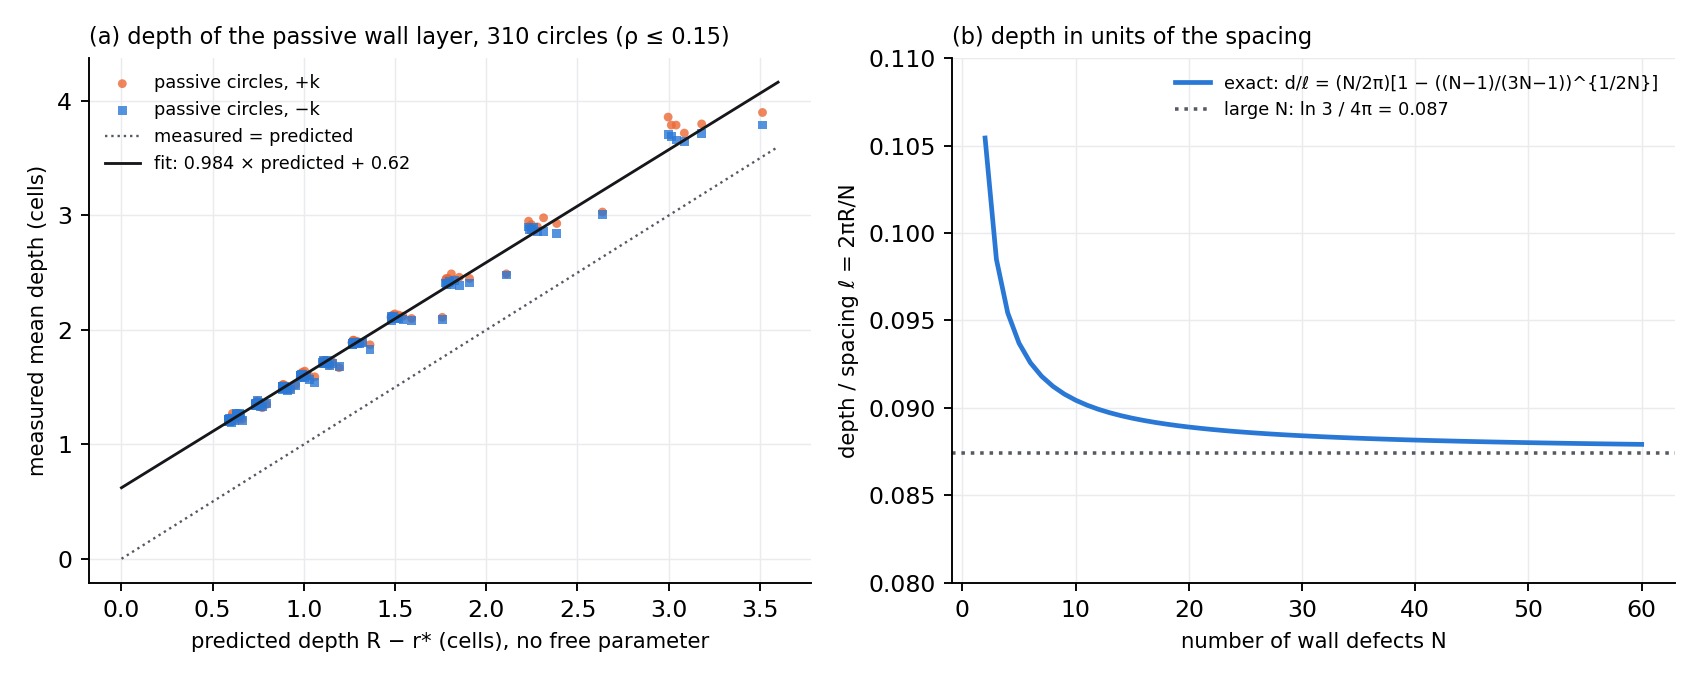
\includegraphics[width=\textwidth]{depth_law.png}
\caption{(a) Measured mean depth of the imposed defects in 310 passive circles ($\rho\le0.15$, both signs) against the parameter-free prediction of
Eq.~\eqref{eq:depth}: measured $=0.984\times$ predicted $+\,0.62$ cells, correlation 0.996. The offset (0.61 cells, IQR 0.60--0.62, the same for
both signs) is where the cell-based anchoring places the effective wall. (b) Depth in units of the spacing against $N$.}\label{fig:depthlaw}
\end{figure}
With a bulk charge $Q_b$ at the centre (the active layer) the minimum becomes $r^*=R[(N-1+2Q_b/q)/(3N-1+2Q_b/q)]^{1/2N}$ (verified), so a $+1$
bulk pushes the layer slightly closer to the wall.

\subsection{Approach of a bulk defect to the wall layer}
Equation~\eqref{eq:ring} along a radius gives the energy of a bulk $+\half$ approaching the $-\half$ wall layer of a mirror circle ($k=-6$,
$R=1.43\,\la$, 14 sites at the depth of Eq.~\eqref{eq:depth} plus the 0.61-cell offset), compared with a free $\pm\half$ pair.
\begin{figure}[H]\centering
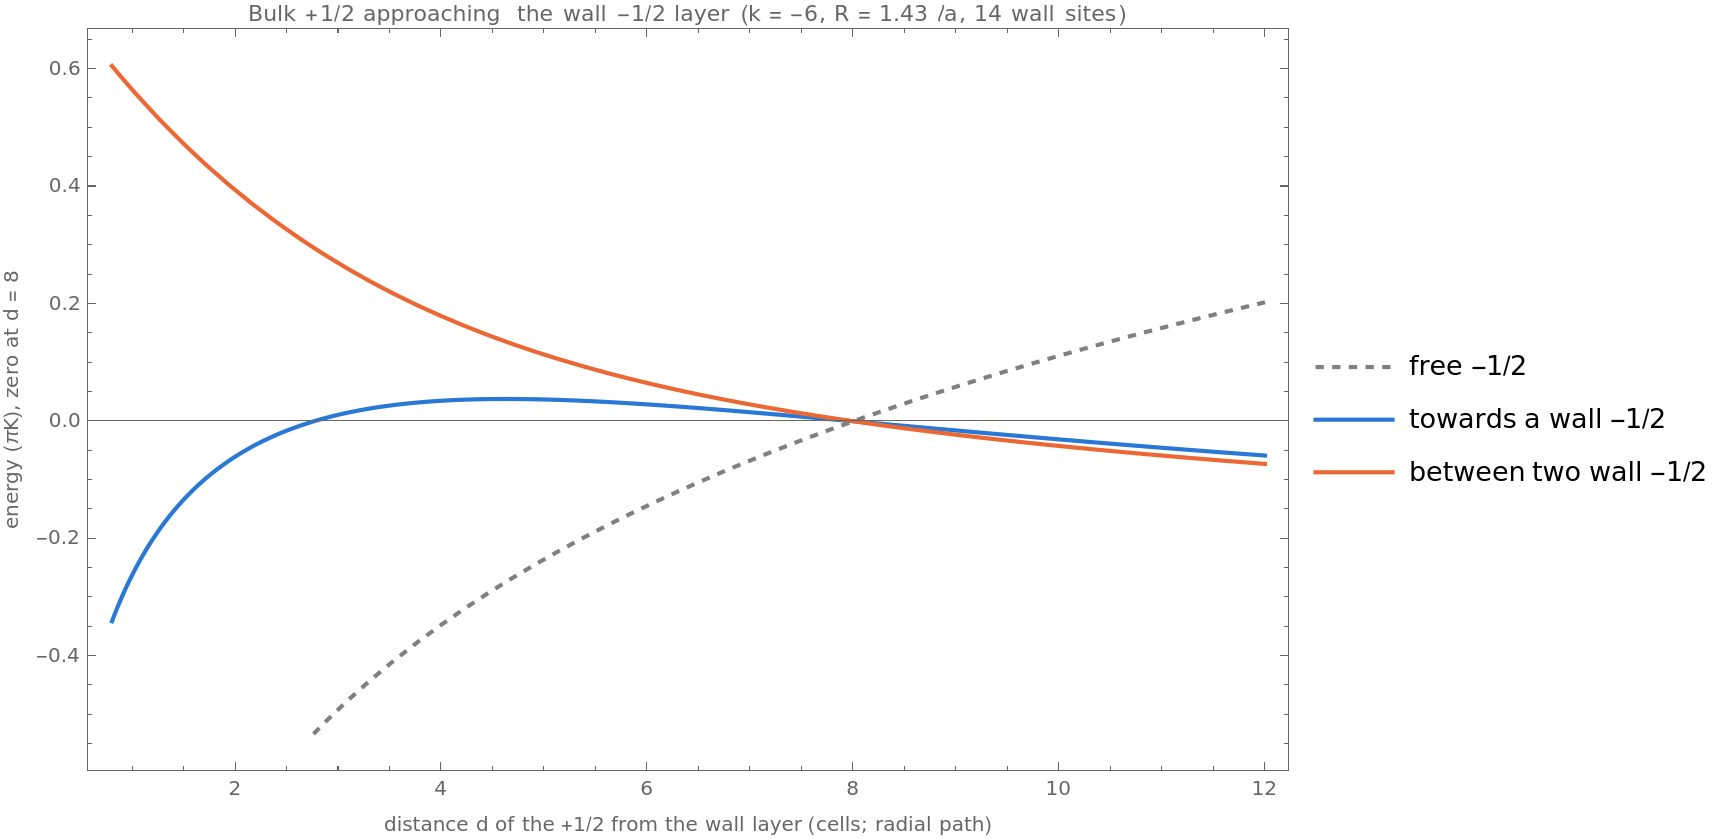
\includegraphics[width=0.85\textwidth]{approach_energy.png}
\caption{Energy of a bulk $+\half$ against its distance from the wall layer along a radius (zero at 8 cells): towards a wall $-\half$ (blue), towards
the gap between two wall $-\half$ (orange), and towards a free $-\half$ (dashed).}\label{fig:approach}
\end{figure}
\begin{table}[H]\centering\small
\caption{Energy released (in $\pi K$) as the $+\half$ moves inwards, theory, and the measured counterpart (shielding test, Sec.~\ref{sec:shield}).}\label{tab:approach}
\begin{tabular}{lccc}\toprule
& towards a free $-\half$ & towards a wall $-\half$ & ratio\\\midrule
theory, from 8 to 4 cells & 0.35 & $-0.03$ (small barrier) & --\\
theory, from 4 to 1 cell & 0.69 & 0.30 & 0.43\\
simulation: encounters reaching $\le2$ cells & 57\% & 28\% & 0.49\\
simulation: encounters ending in annihilation & 53\% & 22\% & 0.41\\\bottomrule
\end{tabular}
\end{table}
The layer turns the long-range attraction into a short-range one: towards a wall $-\half$ there is a small barrier ($\approx0.04\,\pi K$ at 4--5
cells) and attraction only within $\approx3$ cells, with less than half the energy gain of a free pair; towards the gap between two wall defects the
bulk $+\half$ is repelled all the way ($+0.6\,\pi K$ at contact). The measured suppression sits, as predicted, mostly in the approach.

\subsection{Ellipses: shielding is imperfect but the leftover field is weak}
For an ellipse with winding uniform in arclength (eMode 2) the conformal map $w(z)=m^{1/4}\,\mathrm{sn}\!\big(\tfrac{2K(m)}{\pi}\arcsin\tfrac zc,m\big)$
($c^2=A^2-B^2$, nome $((A-B)/(A+B))^2$) sends the cavity to the unit disk. The Neumann Green's function with uniform flux is
$G(z,\zeta)=\ln|w-\omega|+\ln|1-w\bar\omega|+H(z)+H(\zeta)$, where $H$ is harmonic with $\partial_nH=2\pi/P-|w'(z)|$ on the wall (a smooth
boundary datum, solved by a Fourier series). Checks: $|w|=1$ on the wall to $10^{-13}$; for $\varepsilon\to1$ the relaxed ring depth (1.33 cells)
equals Eq.~\eqref{eq:depth} (1.328). Twelve passive $+\half$ were relaxed (from two ring orientations; equal energies), then a bulk test charge
was placed inside.
\begin{table}[H]\centering\small
\caption{Ellipses of area 2500 with 12 $+\half$ ($k=6$), passive equilibrium. Spacing: density ratio flank gap/tip gap (uniform 1, conductor
$\varepsilon$). Shielding: range of the energy that the wall layer (with its images and the boundary winding) gives a bulk $+\half$, inside the
0.6 and 0.8 levels, and centre minus tip regions.}\label{tab:ellth}
\begin{tabular}{lcccc}\toprule
& circle & $\varepsilon=1.2$ & $\varepsilon=1.5$ & $\varepsilon=2.0$\\\midrule
relaxed depth (cells) & 1.33 & 1.33--1.35 & 1.35--1.39 & 1.42--1.55\\
spacing, density ratio (theory / passive simulation) & 1.00 / -- & 1.00 / 0.97 & 1.01 / 0.98 & 1.01 / 0.98\\
layer energy range, inside 0.6 level ($\pi K$) & 0.003 & 0.008 & 0.021 & 0.059\\
layer energy range, inside 0.8 level ($\pi K$) & 0.12 & 0.15 & 0.22 & 0.33\\
centre minus tip regions ($\pi K$) & 0.003 & $-0.002$ & $-0.010$ & $-0.019$\\\bottomrule
\end{tabular}
\end{table}
\begin{itemize}
  \item The passive layer stays evenly spaced in arclength (theory and simulation agree); it does not adopt the screening (conductor) distribution.
  \item The shielding of an ellipse is therefore imperfect: the leftover field in the inner part grows $\approx20\times$ from the circle to
        $\varepsilon=2$. It stays an order of magnitude below the approach energies near the wall ($\lesssim0.06\,\pi K\approx6\,k_BT$ in the inner 60\%, pushing a
        bulk $+\half$ slightly towards the centre), but is not negligible compared with $k_BT$ (Sec.~\ref{sec:frank}).
  \item \textbf{Consequence:} elastic shielding explains the circle (the bulk is blind to $k$; the passive depth; the screened approach), but the
        unscreened elastic field in an ellipse is probably too weak to destroy the layer on its own. The loss of the layer in elongated cavities is more
        likely driven by the flow: two vortices instead of one, wandering and escaping wall defects, depleted tips (Secs.~\ref{sec:slattice},
        \ref{sec:sflow}). The negative-winding ellipses (running) test this: $-\half$ are not self-propelled.
\end{itemize}
\subsection{Energy scale: the Frank constant of the MPCD nematic}\label{sec:frank}
The Frank constants are not inputs of nematic MPCD; they were measured from the equilibrium director fluctuations of a passive, defect-free,
periodic $64\times64$ box (two seeds; size check $96\times96$, one seed) with the cavity parameters (density 20, mean-field potential $U=10\,k_BT$, collision operator 21 at zero activity),
initially aligned along $x$: for a director along $x$, $Ak_BT/\langle|\theta_{\mathbf q}|^2\rangle=K_1q_y^2+K_3q_x^2$, fitted over $|q|<0.8$ with a
constant for the cell-level noise (\texttt{runs/Kcalib/frank\_constant.py}, 900 frames per run, $\langle S\rangle=0.876$, no defects; the mean director stays within $16^\circ$ of $x$
in every frame). The spectrum is linear in $q^2$ along both axes, with splay stiffer than bend at every wavenumber (Fig.~\ref{fig:frank}); single modes
scatter by up to $12\,k_BT$ at $q<0.3$ (one mode each), which the two-constant fit averages.
\begin{table}[H]\centering\small
\caption{Frank constants of the 2D MPCD nematic ($U=10\,k_BT$, density 20; $k_BT$; seeds 1, 2: $64\times64$). \texttt{reports/master/data/frank\_constants.txt}.}\label{tab:frank}
\begin{tabular}{lccc}\toprule
& $K_1$ (splay) & $K_3$ (bend) & one-constant $K=(K_1+K_3)/2$\\\midrule
seed 1 & 42.1 & 22.6 & 32.4\\
seed 2 & 41.9 & 23.5 & 32.7\\
$96\times96$, seed 1 & 41.5 & 23.0 & 32.3\\\bottomrule
\end{tabular}
\end{table}
\begin{figure}[H]\centering
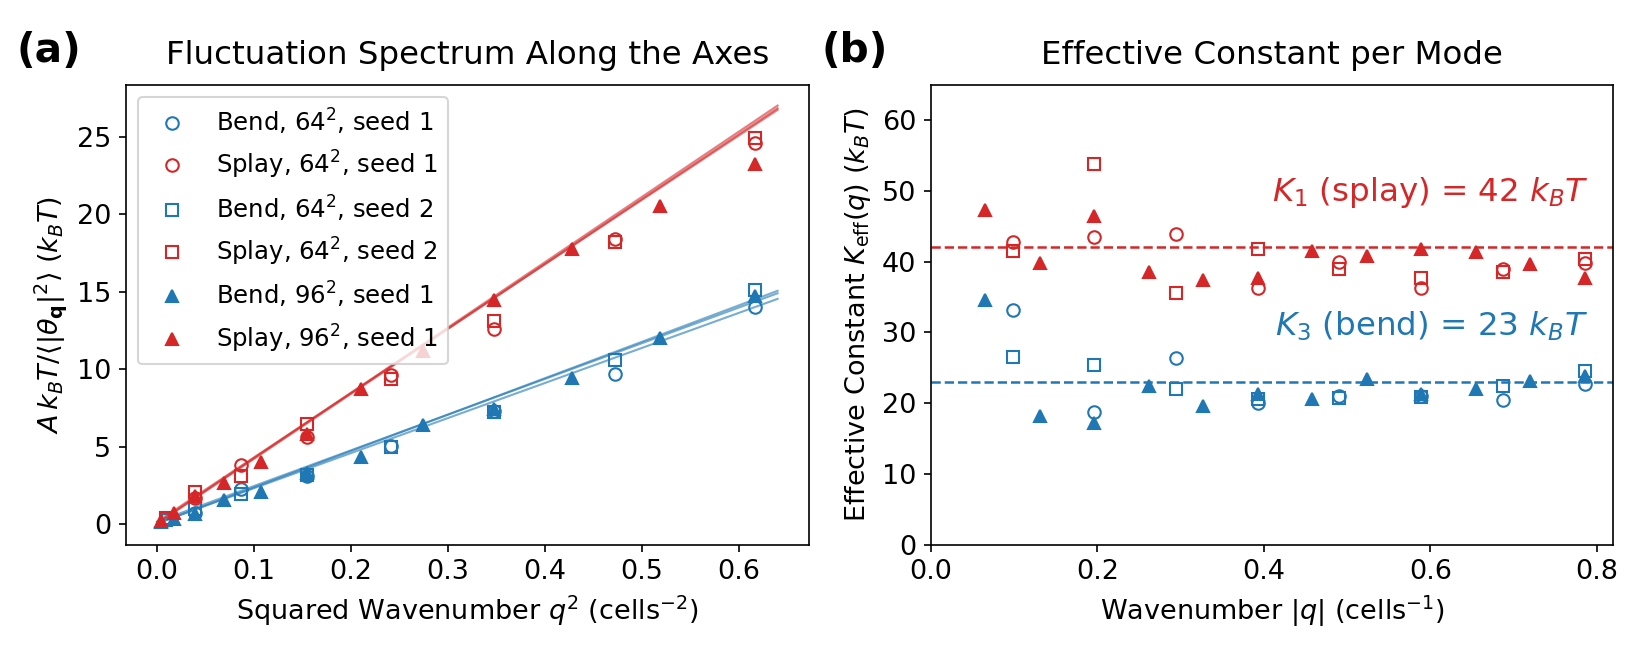
\includegraphics[width=\textwidth]{frank_spectrum.png}
\caption{Director fluctuations of the passive periodic boxes ($U=10\,k_BT$, density 20, director along $x$). (a) Inverse mode amplitude
$A\,k_BT/\langle|\theta_{\mathbf q}|^2\rangle$ ($A$ the box area) against $q^2$ along the bend ($q_x$, blue) and splay ($q_y$, red) axes; lines: the
two-constant fit $K_1q_y^2+K_3q_x^2+c$ of each box over $|q|<0.8$ ($c$ the white noise of the cell estimate). (b) Effective constant of each mode,
$K_\mathrm{eff}=A\,k_BT/(q^2\langle|\theta_{\mathbf q}|^2\rangle)$; dashed: $K_1=42$ and $K_3=23\,k_BT$. Open symbols $64\times64$ (circles seed 1,
squares seed 2), filled triangles $96\times96$. \texttt{scripts/fig\_frank.py}; \texttt{data/frank\_constants.txt}.}\label{fig:frank}
\end{figure}
In 2D the elasticity is not isotropic (splay $\approx1.8\times$ bend; in 3D the original algorithm paper reports isotropic constants,
$K_i\approx113\,U$ per unit length (T.~N.~Shendruk and J.~M.~Yeomans, Soft Matter \textbf{11}, 5101 (2015))). With $K\approx32\,k_BT$, $\pi K\approx100\,k_BT$: the approach barrier towards a wall
$-\half$ is $\approx4\,k_BT$, the pull from 4 to 1 cell $\approx30\,k_BT$ (free pair $\approx70$), the repulsion between two wall defects $\approx60\,k_BT$,
and the leftover field inside an $\varepsilon=2$ ellipse $\approx6\,k_BT$ in the inner 60\% and $\approx33\,k_BT$ inside the 0.8 level (circle: $0.3$).
Near the wall the shielding energies are tens of $k_BT$, so thermal noise plays no role and activity moves the defects; whether the leftover field in
an ellipse is weak has to be judged against the active driving, not against $k_BT$. \emph{Activity in the same units} (from the code of collision operator 21): each particle in a cell is kicked by $\pm\zeta N_\mathrm{cell}\cdot\half\cdot\Delta t$
along the director, opposite on the two sides of a plane through the centre of mass (sigmoid factor $\half$ at the mean density), i.e.\ a force of
$\approx0.7$ per particle and a force dipole of $\approx3.5$ per cell: an active stress $\zeta_\mathrm{eff}Q$ with $\zeta_\mathrm{eff}\approx4$, not the bare
$\zeta=0.07$. Then $\sqrt{K/\zeta_\mathrm{eff}}\approx2.8$ cells and $\la\approx8\sqrt{K/\zeta_\mathrm{eff}}$, the usual ratio in continuum simulations.
(An earlier version compared $\sqrt{K/\zeta}$ with the bare $\zeta$; that agreement was a coincidence.)

\subsection{Hydrodynamics: Stokes model of the defect forces}\label{sec:hydro}
\noindent\fbox{\parbox{0.97\textwidth}{\textbf{Correction (2026-10-07): sign error in this subsection and in Sec.~\ref{sec:fluct} (stage 2).}
The defect angle written by the code is the direction of $\nabla\!\cdot Q$ (\texttt{topoAngleLocal}), which for a $+\half$ points to its
\emph{tail} (splay side). Free bulk $+\half$ move \emph{against} this angle (mean step $-0.56$ to $-0.70$ cells per 2 time units, 66--72\% of steps,
$\approx60\sigma$; \texttt{theory/fluct/pinning/head\_convention.py}), as expected for extensile activity: the head, the self-propulsion and the active
force on the fluid all point along $-\hat e_\psi$. All $+\half$ forces below were placed along $+\hat e_\psi$. Consequences:
(i) wall $+\half$ have their tails at the wall and their heads pointing into the bulk, leaning \emph{upstream} (consistent with the upstream drift of
wall defects); their own active forces \emph{oppose} the circulation. The large variance explained by the wall term reflects the tilt being locked to the
flow, not the wall layer driving it; with physical signs a non-negative fit gives the wall layer zero weight. (ii) Bulk $+\half$ drive the circulation
(correlation $+0.5$ in circles) but, as point forces, explain only 6--21\% of the flow variance and do not predict the vortex number in ellipses.
(iii) In the feedback analysis the force reverses, so the wall layer \emph{damps} all tilt patterns, the one-vortex pattern most. Statements below that
the wall layer sustains the circulation are withdrawn pending a model built on the full active force $-\zeta_\mathrm{eff}\nabla\!\cdot Q$ of the
measured director field.}}

\emph{Idea (B.~Loewe):} treat the defects as point forces in a Stokes fluid with no-slip walls, their strength set by the activity. A $+\half$
exerts a net force along its axis, $\mathbf F=\zeta_\mathrm{eff}\!\int\!\nabla\!\cdot\!Q\,dA=\pi\zeta_\mathrm{eff}S\rho_\mathrm{cut}\,\hat{\mathbf e}$
(for an ideal $+\half$, $\nabla\!\cdot\!Q=S/(2r)$ along its axis, $\rho_\mathrm{cut}$ the size of its distorted region); a $-\half$ exerts no net force and
is modelled as three inward forces at $120^\circ$ (a force tripole, as in Norton et al.). Solved with finite elements in Mathematica (velocity and pressure,
no-slip disk, forces smeared over $\sigma=1.5$ cells; \texttt{reports/master/theory/stokes\_circle.wl}, \texttt{stokes\_frames/}).
\begin{figure}[H]\centering
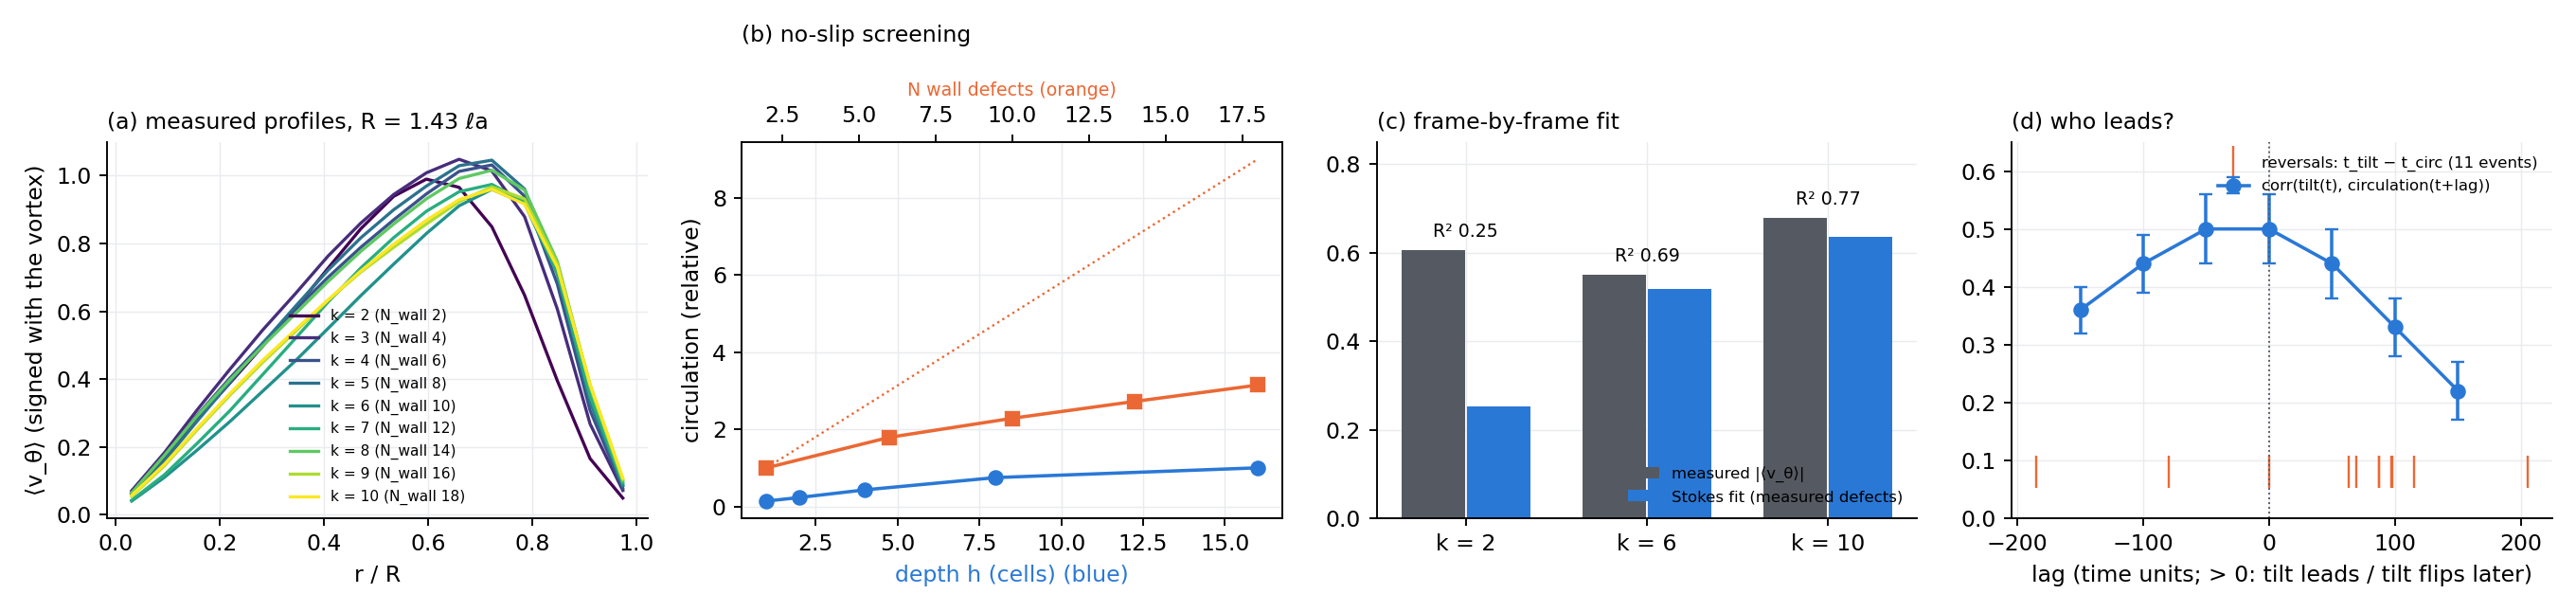
\includegraphics[width=\textwidth]{hydro_circle.png}
\caption{\textbf{Hydrodynamics of the wall layer in circles} ($R=1.43\,\la$). (a) Measured azimuthal velocity profiles for $k=2\dots10$ (fixed-radius scan,
seeds 2--3): the vortex is the same for 2 to 18 wall defects. (b) Static Stokes model: circulation driven by one tangential force against its depth
from the no-slip wall (blue, bottom axis), and by a wall layer of $N$ tilted $+\half$ at the predicted depths (orange, top axis; dotted: proportional to $N$);
both relative. (c) Circulation of the measured flow and of the Stokes flow of the measured defects (frame-by-frame fit), with the fraction of the
flow-field variance explained. (d) Timing: cross-correlation of the fluctuations of wall tilt and circulation (blue; lag $>0$: tilt leads), and the
delay of the tilt reversal after the circulation reversal at 11 vortex reversals ($\zeta=0.05$; orange ticks; $>0$: tilt flips later).}\label{fig:hydro}
\end{figure}
\begin{figure}[H]\centering
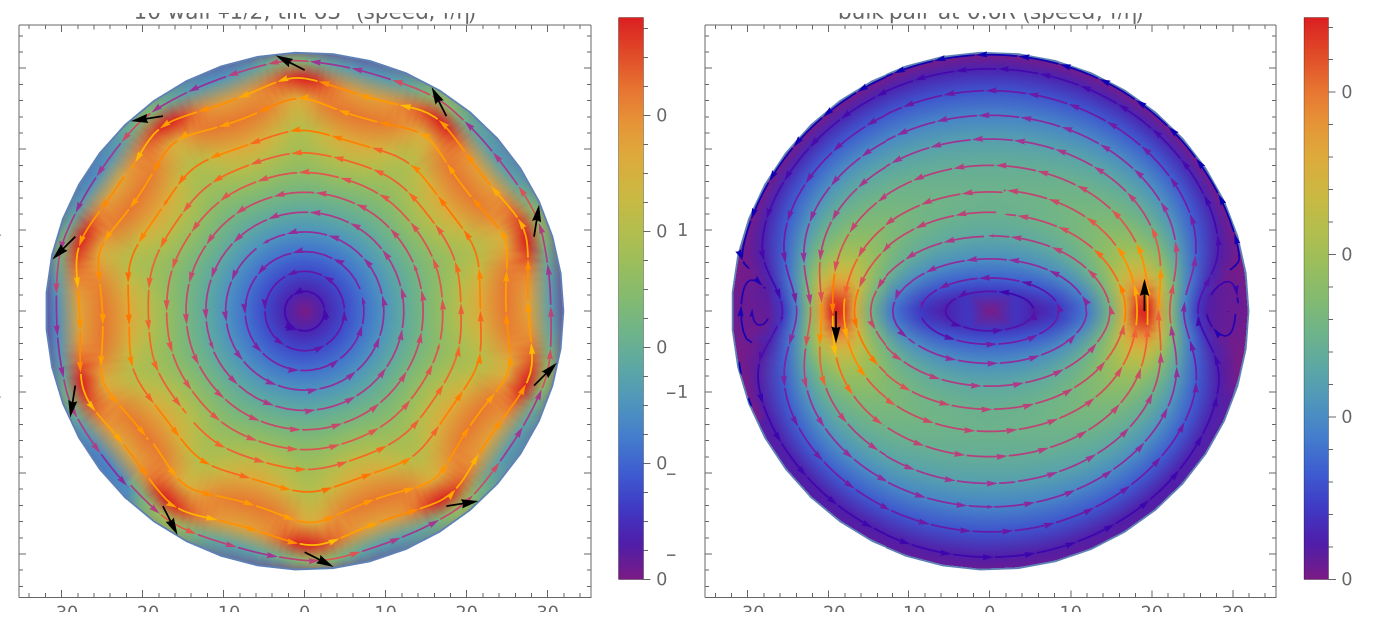
\includegraphics[width=0.85\textwidth]{stokes_circle_fields.png}
\caption{Static Stokes flows (speed in units of $f/\eta$): 10 wall $+\half$ tilted by $63^\circ$ (left) and a bulk pair of co-rotating $+\half$ at $0.6R$
(right).}\label{fig:stokesfields}
\end{figure}
\begin{itemize}
  \item \textbf{No-slip screening.} A force 1--2 cells from the wall drives 5--7$\times$ less circulation than one deep inside. Adding wall defects
        also pulls the layer closer to the wall (depth 5 $\to$ 1.5 cells for $N=2\to18$), so 9$\times$ more wall defects give only 3$\times$ more
        circulation (Fig.~\ref{fig:hydro}b). The $-\half$ tripoles produce essentially no circulation.
  \item \textbf{Measured flow, measured defects.} For each 50-time-unit flow interval the measured defects (every 5th defect frame) were turned into
        forces and the measured velocity field was regressed on the Stokes flows of the wall $+\half$, bulk $+\half$ and $-\half$. At $k=6$ and 10 the
        wall layer alone explains 67\% and 76\% of the flow field, the bulk $+\half$ 8\%, the tripoles nothing; the model circulation is 0.52 and 0.64
        against 0.55 and 0.68 measured. At $k=2$ the model fails (25\% explained, circulation 0.25 against 0.61). The fitted bulk coefficient is negative
        (not understood).
  \item \textbf{The force is of the right size.} The fitted force per wall defect is $f/\eta=20$, 11.5, 9.5 for $k=2$, 6, 10. With the active stress of
        collision operator 21, $\zeta_\mathrm{eff}\approx4$ (Sec.~\ref{sec:frank}), and the MPCD viscosity $\eta\approx17$ (2D formulas for density 20,
        $\Delta t=0.1$: kinetic 1.1, collisional 15.8), this means $\rho_\mathrm{cut}\approx31$, 18, 15 cells: between half the defect spacing and the cavity
        radius, shrinking as the wall gets crowded. The weaker push of a crowded layer, together with the screening, keeps the circulation independent of $k$.
  \item \textbf{But the vortex leads in time.} Fluctuations of wall tilt and circulation move together within one flow interval, with a slight asymmetry
        towards the circulation changing first (correlation 0.36 at $-150$ against 0.22 at $+150$ time units). At 11 vortex reversals (activity 0.05,
        $k=8$--10) the circulation flipped first in 9, the tilt following by a median of $\approx90$ time units.
  \item \textbf{Reading: two-way coupling.} The vortex sets the wall tilt; once tilted, the wall layer's active forces sustain most of the circulation.
        Reversals start elsewhere (the bulk). In an elongated cavity, once the flow organises into two vortices the wall layer loses the coherent tilt
        that sustains a single vortex (Part~III).
\end{itemize}
\paragraph{Ellipses.} \emph{Static:} a coherently tilted wall layer (10 $+\half$ evenly spaced in arclength at depth 1.5, all tilted $63^\circ$ the same way)
drives a \emph{single} vortex in every ellipse of area 2500: both halves rotate the same way, and the whole-cavity rotation drops only from 0.050 (circle)
to 0.033 $f/\eta$ ($\varepsilon=2$) (Fig.~\ref{fig:stokesell}). Elongation alone does not split the flow driven by the layer.
\begin{figure}[H]\centering
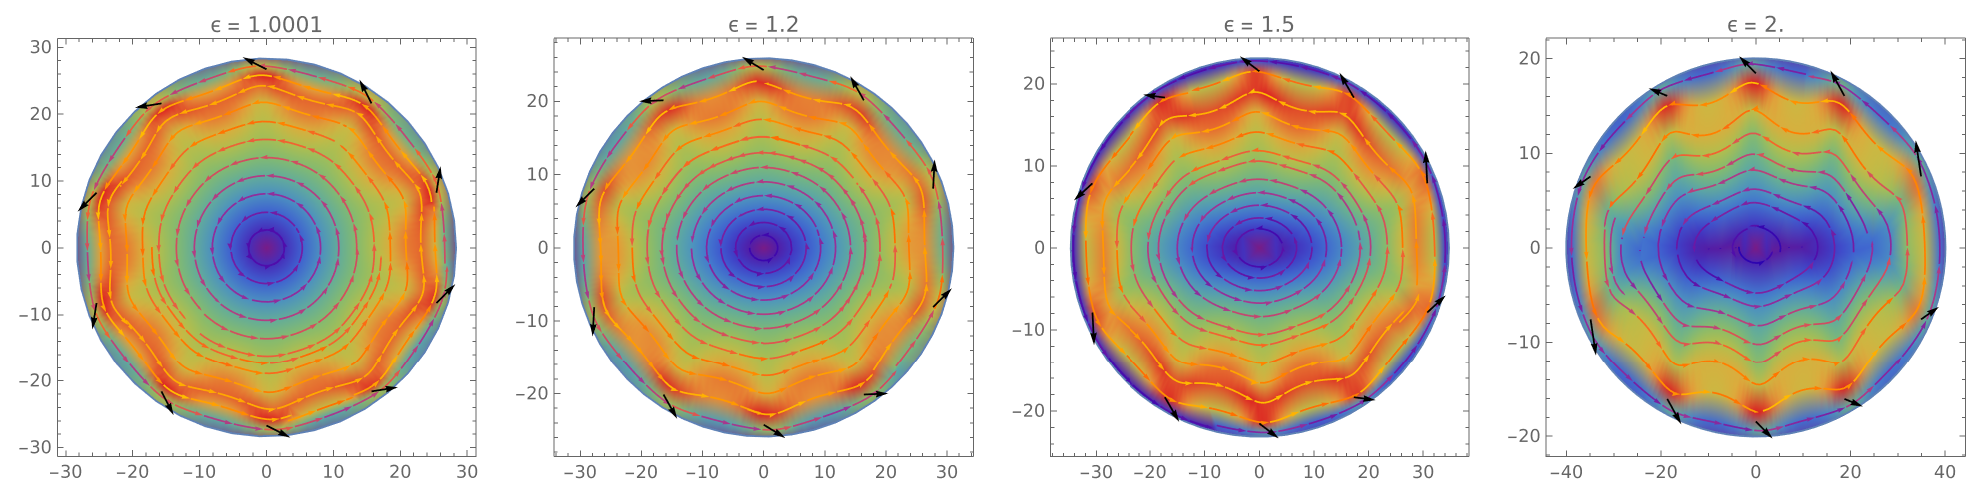
\includegraphics[width=\textwidth]{stokes_ellipse_static.png}
\caption{Stokes flow (speed, $f/\eta$) of a coherently tilted wall layer in a circle and ellipses $\varepsilon=1.2$, 1.5, 2.0 of the same area: a single vortex in all.}\label{fig:stokesell}
\end{figure}
\noindent\emph{Measured defects} (positive-winding ellipses, seed 1, 40 flow intervals of 100 time units each, same fit as for circles):
\begin{table}[H]\centering\small
\caption{Ellipses: Stokes fit of the measured flow on the forces of the measured defects. Half-cavity rotation: mean azimuthal velocity about the centroid of
each half; correlation over time between model and measurement.}\label{tab:hydroell}
\begin{adjustbox}{max width=\textwidth}
\begin{tabular}{lccc}\toprule
& $\varepsilon=1.2$ & $\varepsilon=1.5$ & $\varepsilon=2.0$\\\midrule
measured: halves rotating the same way & 100\% & 28\% & 45\%\\
measured: whole-cavity rotation & 0.57 & 0.26 & 0.09\\
flow variance explained: all / wall $+\half$ only / bulk $+\half$ only & 0.72 / 0.70 / 0.21 & 0.45 / 0.39 / 0.06 & 0.34 / 0.23 / 0.11\\
fitted $f/\eta$ per wall defect & 10.0 & 9.5 & 7.6\\
half-rotation, correlation model--measured (left / right) & 0.25 / 0.43 & 0.94 / 0.94 & 0.85 / 0.86\\
model: halves rotating the same way & 100\% & 40\% & 55\%\\\bottomrule
\end{tabular}
\end{adjustbox}
\end{table}
\begin{itemize}
  \item The measured wall defects reproduce the two-vortex dynamics of the elongated ellipses (half-rotation correlation 0.85--0.94, counter-rotation about
        right): their tilts follow the local vortex, and their forces reinforce the two-vortex flow.
  \item Since a coherently tilted layer would drive a single vortex, the two-vortex state is not imposed by the layer; it comes from the bulk, and the
        wall tilts follow, as the timing test in circles indicates.
  \item The wall layer matters less as the cavity elongates: it explains 70\% of the flow at $\varepsilon=1.2$ and 23\% at $\varepsilon=2.0$, while
        defects leave the wall and the bulk drives more of the flow. One seed per shape; the bulk coefficient is again negative.
\end{itemize}
\noindent\emph{Non-uniform tilts} (\texttt{theory/stokes\_tilt\_modes.wl}; same layer, 10 $+\half$ at depth 1.5, area 2500).
\begin{table}[H]\centering\small
\caption{Static Stokes flow of the wall layer with two tilt patterns: coherent (all $+63^\circ$) and split (left half $+63^\circ$, right half $-63^\circ$).
Rotation (units $f/\eta$) about the centroid of the left half, the right half and the whole cavity. At $\varepsilon=1.5$ one defect sits at $x\approx0$ and is
assigned to one half, hence the asymmetry.}\label{tab:tiltsplit}
\begin{tabular}{lccc}\toprule
$\varepsilon$ & coherent: left / right / whole & split: left / right / whole & split/coherent per half\\\midrule
1.0 & 0.039 / 0.039 / 0.050 & 0.026 / $-0.026$ / 0.000 & 0.68\\
1.2 & 0.040 / 0.040 / 0.048 & 0.029 / $-0.029$ / 0.000 & 0.73\\
1.5 & 0.038 / 0.038 / 0.043 & 0.036 / $-0.027$ / 0.013 & 0.83\\
2.0 & 0.032 / 0.032 / 0.033 & 0.030 / $-0.030$ / 0.000 & 0.94\\\bottomrule
\end{tabular}
\end{table}
\noindent\emph{Feedback modes.} Let $M_{ij}$ be the tangential velocity at wall defect $i$ due to a unit tangential force at wall defect $j$ (symmetric by
Stokes reciprocity). If tilts follow the local tangential flow and the tangential force follows the tilt, $M$ is the linear feedback operator of the
layer; its eigenvectors are the self-reinforcing tilt patterns and the eigenvalues their gains.
\begin{table}[H]\centering\small
\caption{Top eigenvalues of $M$ ($1/\eta$) and their mode type: uniform (all tilts the same, one vortex) or dipolar (left and right halves opposite, two vortices).
In the circle the dipolar mode is degenerate with its rotated partner ($m=1$ pair).}\label{tab:tiltmodes}
\begin{tabular}{lcccc}\toprule
$\varepsilon$ & uniform (1st) & dipolar (2nd) & ratio 1st/2nd & 3rd\\\midrule
1.0 & 0.0737 & 0.0653 & 1.13 & 0.0590\\
1.2 & 0.0735 & 0.0660 & 1.11 & 0.0645\\
1.35 & 0.0733 & 0.0663 & 1.11 & 0.0639\\
1.5 & 0.0730 & 0.0666 & 1.10 & 0.0633\\
1.65 & 0.0726 & 0.0668 & 1.09 & 0.0627\\
1.8 & 0.0722 & 0.0669 & 1.08 & 0.0621\\
2.0 & 0.0717 & 0.0670 & 1.07 & 0.0622\\
2.5 & 0.0705 & 0.0672 & 1.05 & 0.0637\\\bottomrule
\end{tabular}
\end{table}
\begin{itemize}
  \item \textbf{The layer can sustain two vortices.} A split layer drives two counter-rotating vortices with no net rotation, and the price of splitting
        disappears with elongation: per half, the split layer drives 68\% of the coherent rotation in the circle and 94\% at $\varepsilon=2$.
  \item \textbf{But it does not choose them.} The uniform (one-vortex) mode has the largest gain at every aspect ratio up to 2.5, so the wall
        hydrodynamics alone, in the linear feedback picture, would always select one vortex. The dipolar (two-vortex) mode is second from $\varepsilon=1.2$
        on, and its margin shrinks from 13\% (circle) to 5\% ($\varepsilon=2.5$): elongation makes the two states nearly degenerate.
  \item \textbf{Reading.} With nearly degenerate wall modes, a small push from the bulk is enough to select the two-vortex state, and the wall tilts then
        follow and reinforce it. This agrees with the timing in circles (the vortex leads) and with the falling wall share of the flow in ellipses
        (Table~\ref{tab:hydroell}). Measured tilt coherence: 1.00 (circle), 0.98--0.99 ($\varepsilon=1.2$), 0.43 ($\varepsilon=1.5$), 0.34 ($\varepsilon=2.0$).
  \item Caveats: linear, wall layer only, sites evenly spaced and fixed, tangential force only, no noise or elastic torque on the tilt.
\end{itemize}


\paragraph{Limits.} One-constant elasticity; orientation-dependent interactions ignored (the poster notes that they matter at the wall); core
energies and the cell scale enter only through the empirical 0.61-cell offset; no activity or flow. The energy scale $\pi K$ has not yet been
calibrated against the MPCD nematic parameters.

% Wall-lattice fluctuations, mobility and pinning (2026-10-06). Scripts: theory/fluct/
\subsection{Fluctuations, mobility and pinning of the wall lattice}\label{sec:fluct}
\emph{Question (B.~Loewe):} perturb the elastic energy of the wall defects about their equilibrium, add the hydrodynamic forcing, and check the stability
of the layer; on the way, find how much wall defects wander, and use that to build imperfect lattices for the one-vortex/two-vortex question
(Sec.~\ref{sec:hydro}). This subsection collects the passive part (stage~1), the defect mobility, the origin of the pinning, the measured active
wandering, and the imperfect-lattice test (stage~2).

\paragraph{Stage 1: harmonic theory.} Expanding the energy of Eq.~\eqref{eq:Eel} to second order about the relaxed ring (circle) or the relaxed
lattice (ellipse, conformal map), with Hessian $\mathsf H$ in units of $\pi K$, equipartition gives $\langle\delta x\,\delta x^T\rangle=(k_BT/\pi K)\,\mathsf H^{+}$,
projected on the local wall tangent and normal. There is no free parameter once $K$ is fixed. Measurement: passive runs, wall $+\half$ tracked
frame to frame (cyclic relabelling), displacements about each site's mean; ``internal'' removes the collective sliding
(\texttt{theory/fluct/measure\_passive.py}, \texttt{fluct\_theory.wl}).
\begin{itemize}
  \item \textbf{Along the wall the $N$-dependence is exact up to one constant.} Measured/predicted rms with $K=32.5\,k_BT$ (mean of $K_1$, $K_3$) is
        $1.35\pm4\%$ in every case: circles $N=4$--20 ($R=31.83$), $R=27.28$, and passive ellipses $\varepsilon=1.2$, 1.5, 2.0 (Fig.~\ref{fig:fluct}).
        A harmonic fit would give $K_\mathrm{eff}=17.8\,k_BT$.
  \item \textbf{Sliding is a zero mode of the one-constant theory.} A rigid rotation of the ring costs nothing in a circle. In ellipses the sliding
        eigenvalue is $10^{-7}$, $8\times10^{-6}$ and $10^{-4}$ (internal modes from $4\times10^{-3}$), i.e.\ a predicted sliding rms of 84, 10 and
        2.7 cells at $\varepsilon=1.2$, 1.5, 2.0. Measured: 0.3--1 cell in circles and ellipses alike. Something outside the one-constant theory pins
        the lattice (below).
\end{itemize}
\begin{figure}[H]\centering
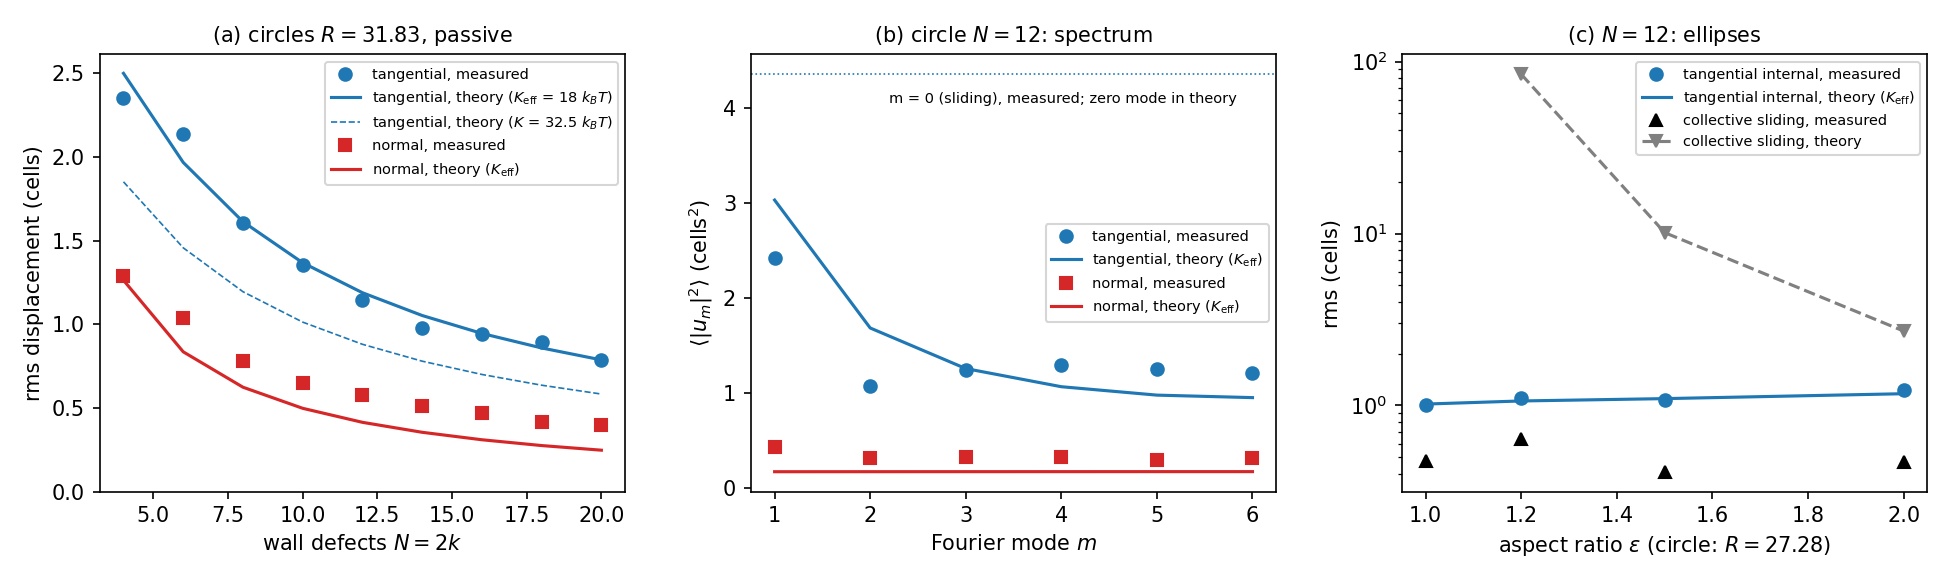
\includegraphics[width=\textwidth]{fluct.png}
\caption{Passive wall-lattice fluctuations, harmonic theory vs measurement. (a) Circles $R=31.83$: rms tangential (internal) and normal displacement
against $N=2k$; dashed: theory with $K=32.5\,k_BT$; solid: with the single fitted $K_\mathrm{eff}=17.8\,k_BT$. (b) Circle $N=12$: spectrum of the
tangential and normal displacements per Fourier mode $m$; dotted: measured $m=0$ (sliding), a zero mode of the theory. (c) $N=12$ ellipses: internal
tangential rms (theory with $K_\mathrm{eff}$) and collective sliding rms, measured (0.4--0.6 cells) and predicted by the one-constant theory (log scale).}\label{fig:fluct}
\end{figure}

\paragraph{Exact potential and the detector.} The harmonic expansion and the raw positions both hide something. (i) The image repulsion is steep
towards the wall and soft towards the bulk. (ii) Both defect trackers (default union-find and legacy, \texttt{pout.c}) write the centre of mass of the cluster of
cells flagged as the core (cell centres at $i+\tfrac12$); the usual cluster is a $2\times2$ block around a cell corner, so 93--98\% of the coordinates are integers and the
rest multiples of $\tfrac16$ or $\tfrac12$ (same in both trackers). The positions are thus quantised to the cell grid, which adds about $1/\sqrt{12}\approx0.29$ cells per
coordinate. Exact Boltzmann sampling (Metropolis) of the full disk energy, with the wall
offset of 0.61 cells from Fig.~\ref{fig:depthlaw} and the sampled positions rounded to the grid like the detector (\texttt{mc\_exact.py},
Fig.~\ref{fig:fluctmc}):
\begin{itemize}
  \item \textbf{Along the wall, $K=K_3=23\,k_BT$ (the measured bend constant) reproduces the data within 2--4\%} for $N=8$--20 (and the mean depth
        within 0.05 cells). The ``$K_\mathrm{eff}$'' of the harmonic fit was mostly detector rounding and mild anharmonicity: tangential displacements of
        wall $+\half$ cost bend.
  \item \textbf{Across the wall a residual remains}, growing for deeper layers: in quadrature $\approx0.15$ cells ($N=20$), 0.35 ($N=12$) and 0.5
        ($N=4$--8). This residual is the target of the random-walk test below.
\end{itemize}
\begin{figure}[H]\centering
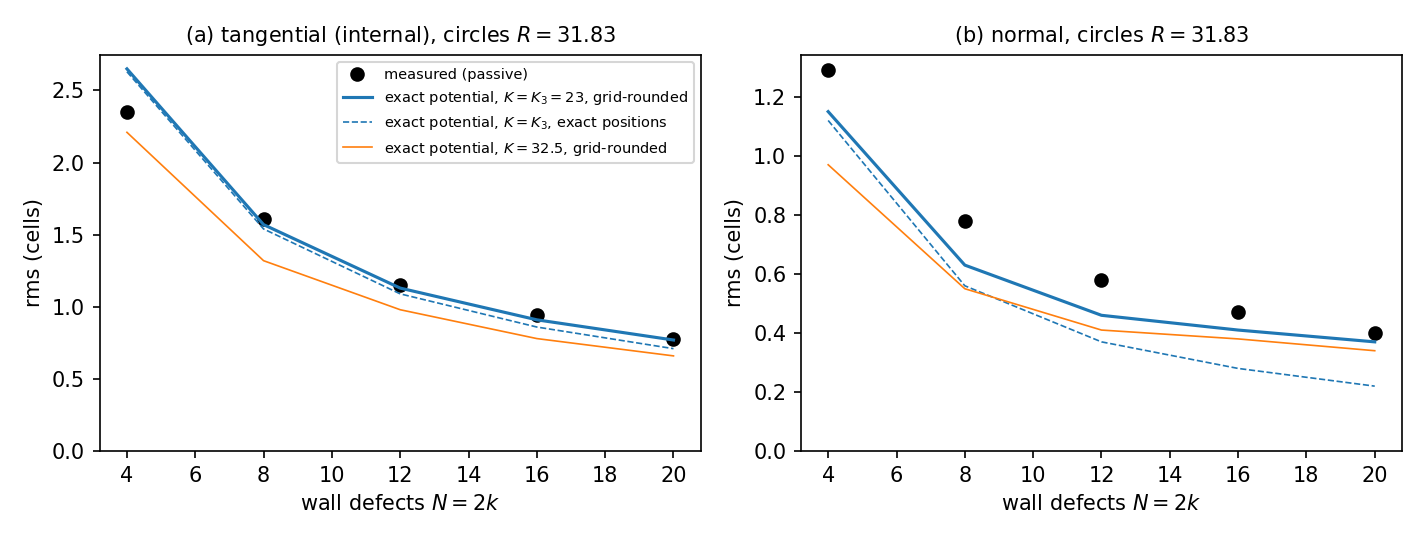
\includegraphics[width=0.85\textwidth]{fluct_mc.png}
\caption{Passive circles $R=31.83$: measured rms displacement (a) along and (b) across the wall against exact Monte Carlo of the full electrostatic
energy (wall offset 0.61). Solid blue: $K=K_3=23\,k_BT$ with positions rounded to the cell grid as in the detector; dashed: exact positions;
orange: $K=32.5\,k_BT$, rounded.}\label{fig:fluctmc}
\end{figure}

\paragraph{Random walks with fluid noise (B.~Loewe's test).} Overdamped Langevin dynamics of the $2k$ wall $+\half$ in the full potential
($K=K_3$, wall offset 0.61, $\mu=0.03$), with white thermal noise plus advection by the cavity fluid: an Ornstein--Uhlenbeck velocity per defect,
tangential and normal, with the variance and correlation time measured at the defect depth in a dedicated passive run
(\texttt{runs/fluidnoise/passive\_R27\_k06}, instantaneous cell velocities every time unit, smoothed over 1.5 cells): rms 0.042--0.049 cells per
time unit, correlation time 0.9--2.6 (shorter near the wall), the same along and across the wall (\texttt{langevin/}). Positions rounded as in
the detector.
\begin{table}[H]\centering\small
\caption{Random walks of the passive wall lattice ($R=31.83$): rms along/across the wall (cells) and median relaxation time of the internal modes.
Fluid noise $\times\lambda$: the measured fluid velocity noise scaled by $\lambda$.}\label{tab:langevin}
\begin{tabular}{lccc}\toprule
& $N=4$ & $N=12$ & $N=20$\\\midrule
measured & 2.35 / 1.29 & 1.15 / 0.58 (37) & 0.78 / 0.40 (12)\\
thermal only & 2.67 / 1.16 & 1.14 / 0.47 (21) & 0.77 / 0.37 (8)\\
thermal + fluid $\times1$ & 2.87 / 1.22 & 1.19 / 0.48 (23) & 0.80 / 0.38 (8)\\
thermal + fluid $\times2$ & 3.34 / 1.43 & 1.36 / 0.52 (23) & 0.89 / 0.39 (8)\\
thermal + fluid $\times4$ & 4.78 / 2.19 & 1.89 / 0.70 (22) & 1.19 / 0.44 (9)\\
fluid only $\times1$ & 1.00 / 0.51 & 0.49 / 0.29 (20) & 0.35 / 0.23 (11)\\\bottomrule
\end{tabular}
\end{table}
\begin{itemize}
  \item At its measured strength the fluid noise adds only 2--5\% to the spreads: its effective diffusivity
        $\langle u^2\rangle\tau\approx0.003$ is a tenth of the thermal $\mu k_BT$. Alone it gives far too little.
  \item Closing the normal gap at $N=12$ would need $\lambda\approx3$, which already overshoots the tangential spread (1.36--1.89 against 1.15).
        The normal excess is therefore not extra isotropic noise: it is specific to the direction across the wall, most likely the detector near the wall
        (the core is distorted by the wall, so its located centre jitters more across than along it), beyond the grid rounding already included.
  \item The relaxation times of the internal modes come out 1.5--1.8$\times$ shorter than measured with $\mu=0.03$, i.e.\ $\mu\approx0.02$ once the
        variances are not inflated by the detector (the model-free estimate below uses the measured, rounding-inflated variances).
\end{itemize}

\paragraph{Mobility.} Overdamped relaxation of mode $m$ with stiffness $k_m=k_BT/\langle|u_m|^2\rangle$ gives
$\mu=\Gamma_m\langle|u_m|^2\rangle/k_BT$, with $\Gamma_m$ the inverse $1/e$ time of the mode autocorrelation. This is model-free: it uses only
measured variances and times (\texttt{mobility.py}). Passive circles $N=8$--20: $\mu\approx0.03$ cells$^2/(k_BT\,\tau)$ (median per run
0.025--0.048), so $D=\mu k_BT\approx0.03$ cells$^2/\tau$. Internal modes relax in 10--40 time units, $m=1$ in 40--230.

\paragraph{The pinning is not the grid.} The MPCD collision grid is randomly shifted every step (\texttt{galInv} = 1), so a fixed-grid pin could
enter only through the detector, and would have a period of about one cell, i.e.\ a random registry in every run. Instead the registry of the wall
lattice with the anchoring pattern is reproducible:
\begin{itemize}
  \item Active circles (all densities and seeds, $k=2$--10): $Z=\langle N_w^{-1}\sum_je^{i(2k-2)\phi_j}\rangle$ has the same phase in different runs,
        mean resultant length 0.43--0.64 against $\approx0.2$ for random phases (e.g.\ $k=6$: 31 runs, Rayleigh $p\approx10^{-4}$), mean phase within
        $\pm0.26$ rad of 0 for every $k$.
  \item Passive circles ($R=13$--64): the phase of $Z_{2k}$ agrees across radii, resultant length 0.65--0.97 against $\approx0.3$. \textbf{But this is
        inherited from the common initial condition} (all production runs start with the director along $y$, \texttt{oDist}=2): eight passive runs
        ($k=6$, $R=31.83$) started along $x$, at $45^\circ$, along $y$ (new seeds) and random settle at different registries, arg $Z$ = $-2.62$ ($x$), $-1.44$
        ($45^\circ$), $-0.07$, $-0.23$, $+0.69$ ($y$), $+0.01$, $+1.20$, $+0.48$ (random), roughly $2(\beta_0-90^\circ)$ for an initial angle $\beta_0$, and only
        creep (0.3--0.5 rad over 3000 time units; Rayleigh $p\approx0.1$ across runs; \texttt{runs/pinning\_ic}, \texttt{ic\_test.py}). The passive registry is
        a symmetry broken by the initial condition and then frozen (B.~Loewe's hypothesis), consistent with a first-order anisotropy barrier below
        $1\,k_BT$ for the incommensurate passive ring. One random start trapped an extra $\pm\half$ pair.
  \item \textbf{The active registry is pinned, independent of the initial condition.} Six active runs ($k=6$, $R=31.83$, $\zeta=0.07$) started random
        ($\times3$), along $x$, at $45^\circ$ and along $y$, plus two production seeds: every run ends at arg $Z=+1.17$ or $-1.17$ rad (concentration 1.00 within
        each run, no creep), i.e.\ at $\pm\tau$ with the measured tilt $\tau=63$--$64^\circ$, one value per circulation sense. Corrected by the lock,
        $D=\arg Z-\tau=+0.03\pm0.07$ in all eight (resultant length 1.00, Rayleigh $p\approx3\times10^{-4}$): the predicted site, whatever the start. Only the
        chirality (sense of rotation) is chosen spontaneously (\texttt{runs/pinning\_ic\_active}, \texttt{ic\_test\_active.py}).
\end{itemize}

\paragraph{Tilt and position are locked.} The anchoring director $\psi=k\phi$ is invariant only under rotations by $2\pi/(2k-2)$. In the one-constant
solution (defects plus same-sign images) a rigid rotation $\alpha$ of the lattice costs nothing but tilts every $+\half$ head, relative to its wall
normal, by $(2k-2)\alpha$; for a defect at the wall, $\text{tilt}_j=(2k-2)\phi_j+\text{const}$. Tests (\texttt{pinning/}):
\begin{itemize}
  \item \textbf{Passive:} the collective tilt follows the collective rotation with slope $0.87$--$0.92\times(2k-2)$, correlation 0.95--0.97
        ($k\ge5$). Along a $2k$ ring the mean tilt steps by $-2\cdot2\pi/N$ per defect ($k=6$: $+41^\circ,-20^\circ,-91^\circ,\dots$), as predicted:
        the passive heads do not all point at the wall.
  \item \textbf{Active ($N=2k-2$, $\approx$150\,000 frames, $k=3$--10):} $D=\arg Z-\bar\tau$ (registry minus mean tilt) is the same in every frame of
        every run, resultant length 0.99, mean 0.00; within runs $\arg Z$ follows $\bar\tau$ with slope 1.04--1.15 (theory 1).
\end{itemize}
So the $2k-2$ sites are the positions where the recorded angle (the tail, $\nabla\!\cdot Q$) points straight at the wall, i.e.\ the head points straight into the bulk, and a wall defect cannot tilt without sliding off its site:
the coherent $63^\circ$ tilt of the active circles shifts the lattice by $63^\circ/(2k-2)$ ($k=6$: 3.5 cells at $R=32$).

\paragraph{What pins the registry: splay $\neq$ bend.} With $K_{1,3}=K\pm\Delta$ the first-order correction to the energy is
$\Delta F=\frac{\Delta}{2}\int(\text{splay}^2-\text{bend}^2)\,dA$ on the exact one-constant field, which depends on the registry. Integrated
numerically with a smooth core cutoff $a$ (\texttt{anisotropy\_pinning.py}; $K_1=42.0$, $K_3=23.1$, $\Delta=9.45\,k_BT$; Fig.~\ref{fig:anisopin}):
\begin{itemize}
  \item \textbf{Active ring} ($2k-2$ wall $+\half$ and a central $+1$): the minimum is exactly at zero tilt (heads at the wall), the measured
        registry. The barrier is 80--110\,$k_BT$ ($k=6$), 45--70 ($k=8$), 100--170 ($k=4$). The curvature predicts a collective rms of 0.45--0.51 cells
        ($k=6$, $R=31.8$, $a=0.5$--2), against 0.29--0.36 measured in the pinned active circles at that radius: the right order and the right site,
        with no free parameter.
  \item \textbf{Passive ring} ($2k$ defects, incommensurate with the $2k-2$-fold pattern): the first-order barrier is only 0.1--1\,$k_BT$ and depends on
        the core cutoff, consistent with the initial-condition test: the passive registry is not pinned but frozen in from the start, its slow creep
        set by the small collective mobility.
  \item In a one-constant model (such as the Q-tensor model of Norton \emph{et al.}) this pinning would be absent: the sliding of the wall lattice
        would be free.
\end{itemize}
\begin{figure}[H]\centering
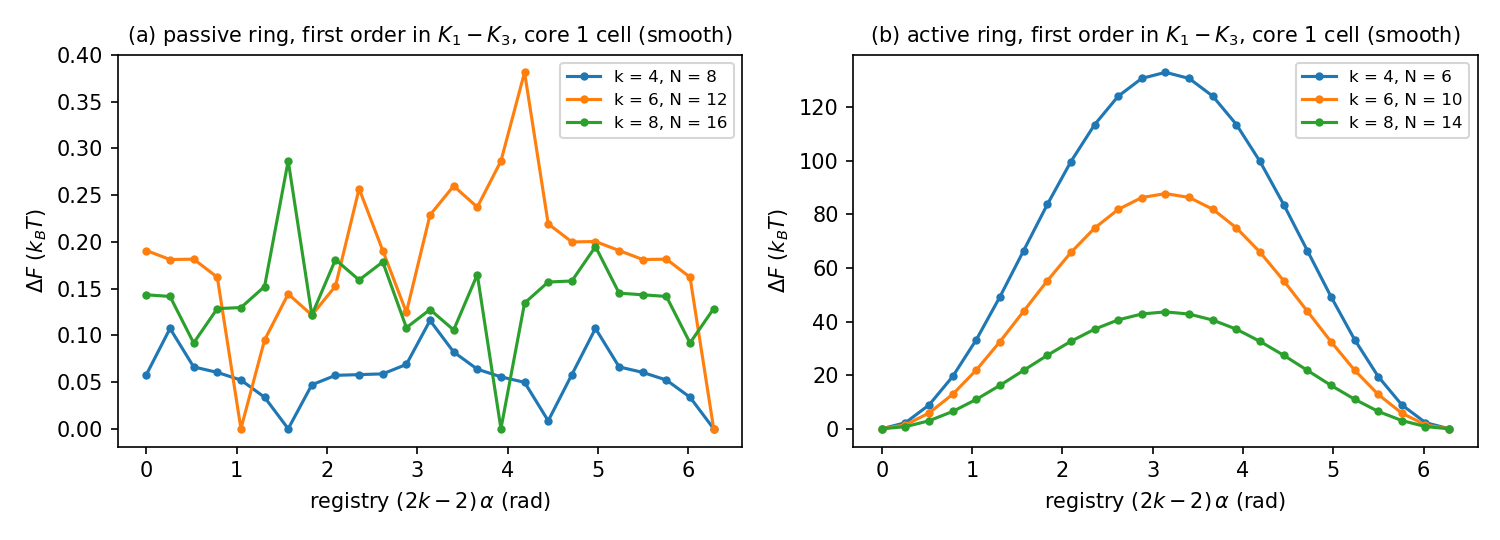
\includegraphics[width=0.9\textwidth]{anisotropy_pinning.png}
\caption{Registry potential of the wall lattice from splay--bend anisotropy (first order in $K_1-K_3$, smooth core cutoff of 1 cell), against
the registry $(2k-2)\alpha$; zero = heads pointing at the wall. (a) Passive ring of $2k$: below $1\,k_BT$. (b) Active ring of $2k-2$ with a
central $+1$: barriers of tens of $k_BT$, minimum at zero tilt.}\label{fig:anisopin}
\end{figure}

\paragraph{How much wall defects wander in active runs.} Disorder is measured as $\sigma_\mathrm{gap}=\mathrm{sd}(g)/\sqrt2$, with $g$ the
arclength gaps between neighbouring wall $+\half$. For independent Gaussian displacements about evenly spaced sites this is exactly $\sigma_t$, the
disorder parameter of the stage-2 ensembles, and needs no tracking (passive check: $\sigma_\mathrm{gap}=1.03$--1.17 against tracked 1.01--1.23;
\texttt{active\_wander.py}, Fig.~\ref{fig:wander}).
\begin{itemize}
  \item \textbf{Active circles} ($k=6$, $R/\ell_a=0.4$--2.2): $\sigma_\mathrm{gap}=0.6$--1.5 cells, the passive level; the wall count is $2k-2=10$ in
        75--93\% of frames. At $R/\ell_a=2.9$ the lattice melts ($\sigma_\mathrm{gap}\approx9$, count $7.6\pm2.2$).
  \item \textbf{Active ellipses:} $\varepsilon=1.2$: $\sigma_\mathrm{gap}=1.3$ (count $9.8\pm0.6$); $\varepsilon=1.5$: 6.3--6.5 (count $7.7\pm1.1$);
        $\varepsilon=2.0$: 8.1--8.4 (count $7.3\pm1.1$), both seeds. The lattice also slides freely (collective rms of tens of cells).
\end{itemize}
The realistic stage-2 disorder is therefore $\sigma_t\approx1$ for circles and $\varepsilon=1.2$, and $\sigma_t\approx6$--8 with 2--3 vacancies for
$\varepsilon=1.5$--2.
\begin{figure}[H]\centering
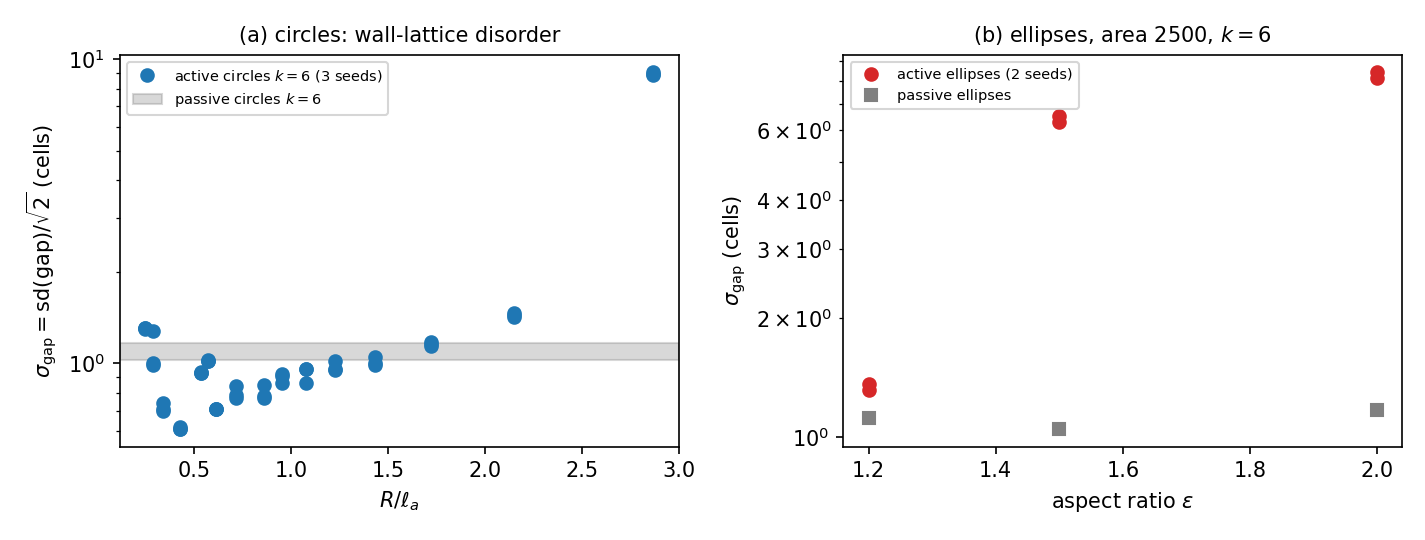
\includegraphics[width=0.9\textwidth]{active_wander.png}
\caption{Wall-lattice disorder $\sigma_\mathrm{gap}$ (log scale). (a) Active circles $k=6$, three seeds, against $R/\ell_a$; grey band: passive circles.
(b) Ellipses of area 2500, $k=6$: active (two seeds) and passive.}\label{fig:wander}
\end{figure}

\paragraph{Stage 2: imperfect lattices.} \textbf{(See the correction box in Sec.~\ref{sec:hydro}: with the physical force direction the feedback is negative, the wall layer damps
every tilt pattern and the one-vortex pattern most; the ``gain ratio'' below then measures how much more strongly one vortex is braked than two.)} For each configuration of wall $+\half$, the Stokes feedback matrix $M_{ij}$ (Sec.~\ref{sec:hydro}) is
computed and its top mode classified as one-vortex or two-vortex by its overlap with the uniform and the left/right-antisymmetric patterns
(\texttt{stage2/}). Gain ratio $=$ largest one-vortex eigenvalue / largest two-vortex eigenvalue (above 1: the layer prefers one vortex).
\begin{itemize}
  \item \textbf{Synthetic disorder (4\,845 configurations).} Lattices of 10 wall $+\half$ (area 2500, depth 1.5), tangential disorder
        $\sigma_t=0.5$--6 cells (normal 0.5), 1--3 vacancies, and the realistic active disorder ($\sigma_t=6$ or 8 with 2 or 3 vacancies), 60--80
        samples per class, $\varepsilon=1$, 1.2, 1.5, 2.0, 2.5. Up to $\varepsilon=1.5$ the top mode is one-vortex in every sample (95\% upper bound
        5--6\% per class); at $\varepsilon=2.0$ only 1/60 in the two most disordered classes. Only at $\varepsilon=2.5$ with realistic disorder does the
        two-vortex mode win in a minority of lattices: 8--15\% ($\sigma_t=6$--8, 2--3 vacancies), 2--5\% for milder disorder (Fig.~\ref{fig:stage2}).
        Disorder spreads the gain ratio but does not lower its median (1.11--1.32 everywhere, perfect lattice 1.13 in the circle, 1.05 at 2.5).
  \item \textbf{Measured wall configurations, two seeds.} One snapshot per flow interval (40 per run): top mode one-vortex in 240/240 snapshots
        ($\varepsilon=1.2$, 1.5, 2.0; seeds 1 and 2), although the measured flow has two vortices in 68--72\% ($\varepsilon=1.5$) and 48--55\%
        ($\varepsilon=2.0$) of the intervals. The gain ratio is not systematically smaller in the two-vortex intervals, and the measured tilt pattern
        barely projects on the predicted top mode (0.16--0.17 against 0.13--0.15 for a random pattern).
  \item \textbf{Reading.} Within the linear tilt-follows-flow feedback the wall layer amplifies one vortex most, whatever its disorder, up to the
        aspect ratios simulated; at $\varepsilon\approx2.5$ disorder begins to make the two-vortex state competitive. The two-vortex state of the
        $\varepsilon=1.5$--2 ellipses is imposed from outside the wall layer (the bulk), consistent with the timing in circles and with the falling wall
        share of the flow (Table~\ref{tab:hydroell}).
\end{itemize}
\begin{figure}[H]\centering
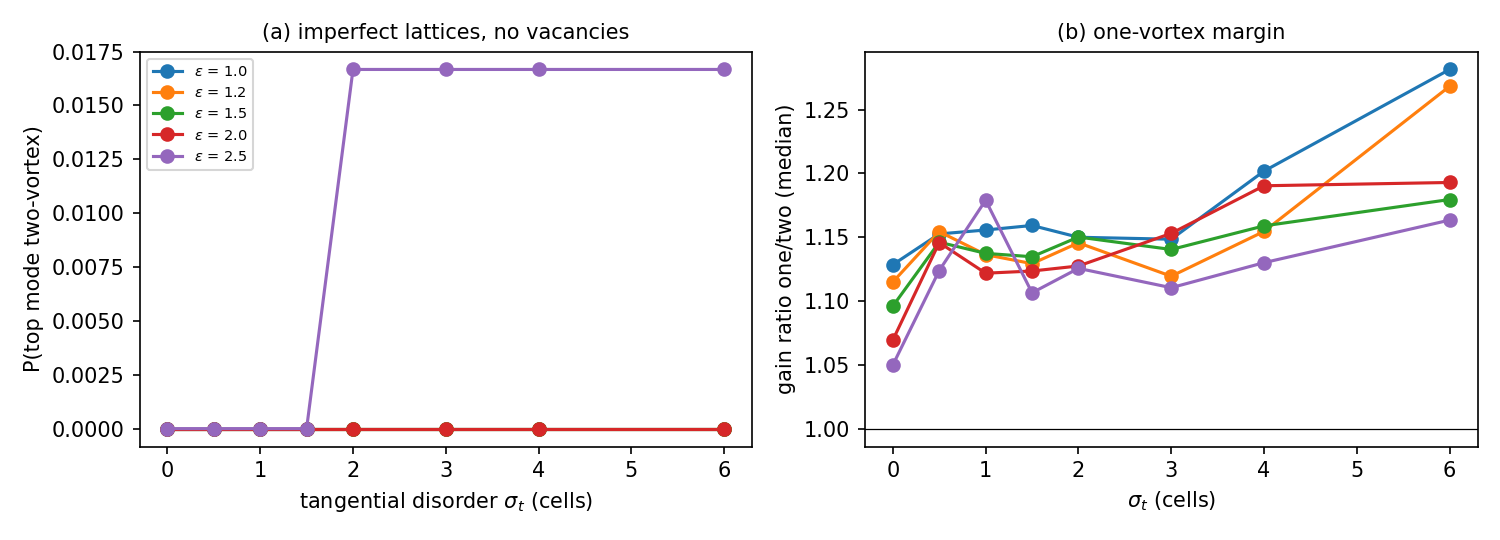
\includegraphics[width=0.9\textwidth]{stage2.png}
\caption{Stage 2. (a) Probability that the top feedback mode of a disordered wall lattice is two-vortex, against the tangential disorder
$\sigma_t$, per aspect ratio (no vacancies). (b) Median gain ratio one-vortex/two-vortex (1: degenerate).}\label{fig:stage2}
\end{figure}


% Director-field Stokes model and the effective boundary condition behind the layer (2026-10-07 night)
\subsection{Hydrodynamics from the full active stress of the measured director field}\label{sec:dirstokes}
After the sign correction (box in Sec.~\ref{sec:hydro}) the point-defect model is replaced by the full active force of the measured director
field, with no defect idealisation and no head/tail convention (\texttt{theory/dirstokes/}). For each flow interval: $Q=S(\mathbf n\mathbf n-\mathbb I/2)$
from the director snapshots at both ends of the interval (averaged, since the flow output is an interval average), force density $\mathbf f=-\nabla\!\cdot Q$
(centred differences inside the cavity, one-sided at the wall), split into a wall band (cell centre within 4 cells of the wall) and the bulk;
Stokes flow with no slip ($\eta=1$, FEM as before) of each part; measured flow $=c_w\mathbf u_w+c_b\mathbf u_b$ fitted per run. Circles
$R=31.83$ ($k=2,6,10$, 40 intervals of 50 time units) and ellipses $\varepsilon=1.2,1.5,2.0$ (two seeds, 40 intervals of 100).
\begin{itemize}
  \item \textbf{One positive coefficient explains most of the flow.} $\mathbf v=c(\mathbf u_w+\mathbf u_b)$ gives $R^2=0.62$--0.72 in circles and
        0.48--0.65 in ellipses, circulation correlation 0.61--0.85, with $c=0.42$--0.67, against $\zeta_\mathrm{eff}/\eta\approx0.24$ from the rough
        calibration (Sec.~\ref{sec:frank}): the right sign and order of magnitude.
  \item \textbf{The bulk drives, the wall band brakes.} Alone, the bulk part gives $R^2=0.47$--0.73 with a positive coefficient; the wall band alone
        gives $R^2\le0.21$ and only with a negative coefficient, its circulation anti-correlates with the measured one ($-0.56$ to $-0.85$), and it carries
        9--17\% of the predicted circulation. The local power $\langle\mathbf f\cdot\mathbf v\rangle$ is positive in both regions, but the flow the wall
        band produces, confined by the no-slip wall, opposes the circulation.
  \item \textbf{The two vortices of elongated ellipses come from the bulk active stress.} The antisymmetric (two-vortex) part of the half-cavity
        rotations predicted by the bulk force correlates with the measured one at 0.87--0.91 ($\varepsilon=1.5$, 2.0, both seeds), and the vortex number is
        right in 72--82\% of the intervals (measured two-vortex fraction 50--68\%). The wall band opposes both the one- and the two-vortex parts.
\end{itemize}
\begin{figure}[H]\centering
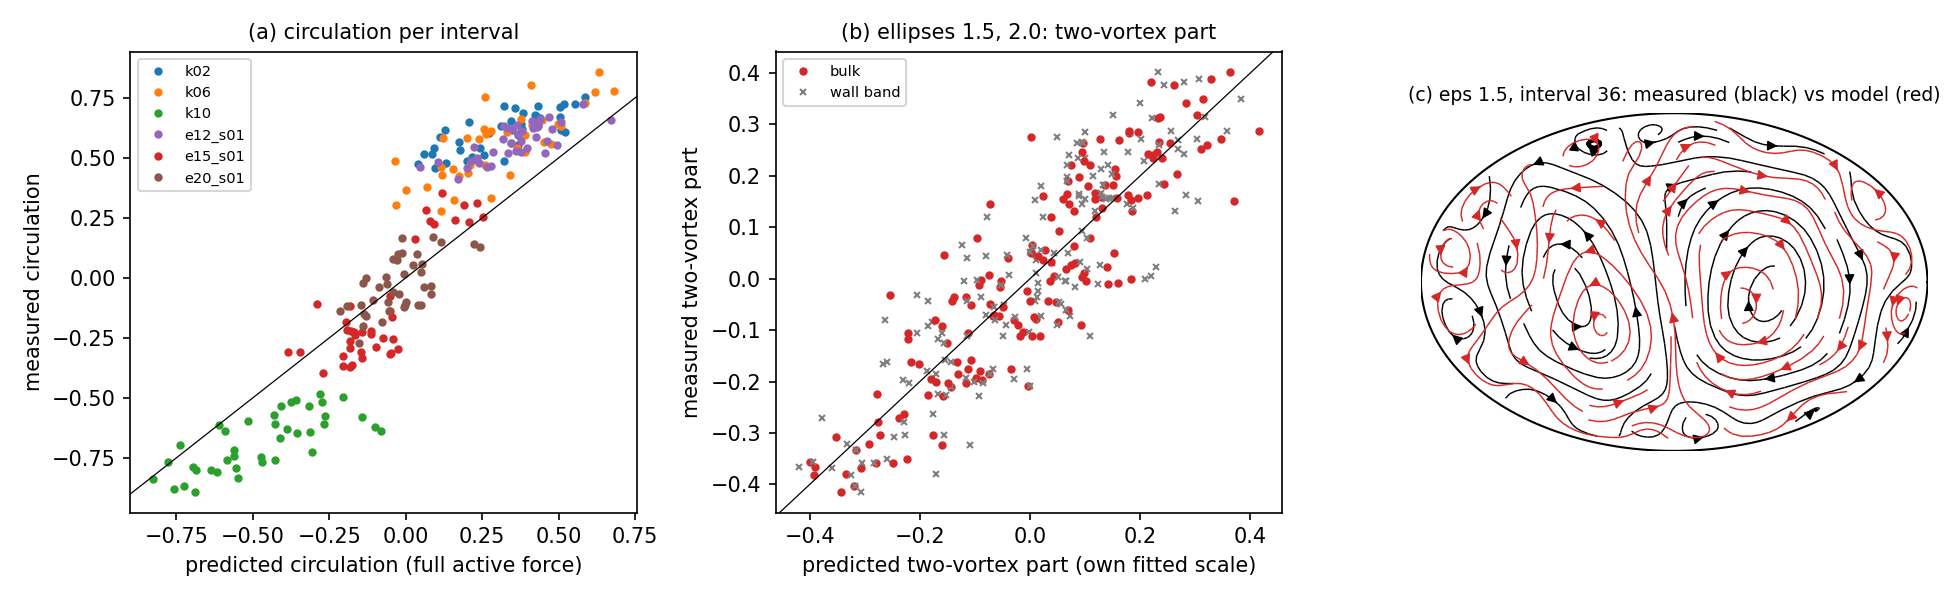
\includegraphics[width=\textwidth]{dirstokes.png}
\caption{Stokes flow of the full measured active force $-\nabla\!\cdot Q$. (a) Cavity circulation per interval, measured against predicted (one fitted
coefficient per run; circles $k=2,6,10$ and ellipses, seed 1). (b) Ellipses $\varepsilon=1.5$, 2.0 (both seeds): two-vortex (antisymmetric) part of the
half-cavity rotations, measured against the bulk-only prediction (red) and the wall-band-only prediction (grey; its fitted scale is negative: the wall band
opposes the measured flow). (c) An interval with two vortices at $\varepsilon=1.5$: measured (black) and predicted (red) streamlines.}\label{fig:dirstokes}
\end{figure}

\subsection{The wall layer as an effective planar boundary}\label{sec:effbc}
\emph{Question (B.~Loewe):} how closely spaced must the tilted wall defects be to act as an effective (planar) boundary condition, and does that give
an independent criterion for the $+1$ bulk? In the one-constant solution the layer's field inside the ring splits into a uniform part
$q_i\arg(-z_i)$ summed over the ring and a modulation that decays as $(r/r_\mathrm{ring})^N\approx e^{-2\pi\delta/\ell}$ with the depth $\delta$ behind the layer
($\ell=2\pi r_\mathrm{ring}/N$, $N=2k-2$). With the anchoring of the code ($\theta=k\phi$ on the wall, \texttt{lc.c}) and the measured registry (tails at the
wall, sites at $\phi_j=2\pi j/N$), the bulk $+1$ sees $\theta=\phi+c$ with (\texttt{theory/effbc/effective\_bc.py}, exact for $k=3,6,10$):
\begin{itemize}
  \item $c=90^\circ$ for an untilted layer: the layer converts the $k$-fold patterned anchoring into an \textbf{effectively planar} (tangential)
        condition of winding 1, the parallel-anchoring problem of Norton \emph{et al.};
  \item $c=90^\circ+\tau/2$ for a layer tilted by $\tau$ (registry shift $\tau/(2k-2)$): a spiral, $121.5^\circ$ at the measured $\tau=63^\circ$;
  \item the modulation falls below 0.1 rad at $\delta=0.25\,\ell$ for every $k$: the bulk sees a smooth effective boundary from $\approx0.34\,\ell$ from the
        wall (ring depth included), i.e.\ at a fraction $2.1/N$ of the radius.
\end{itemize}
\textbf{Self-consistency.} For an extensile $+1$ with $\theta=\phi+c$ the active force has an azimuthal component $\propto\sin(2c-180^\circ)$:
zero for the planar condition, positive (counter-clockwise) for $c=121.5^\circ$. The tilt sign follows the circulation (tilt $+63^\circ$ with counter-clockwise
flow), so a tilted layer turns the effective boundary into a spiral whose active stress drives the same circulation that tilts the layer: a feedback that
runs through the elastic field behind the layer, not through point forces at the wall (which oppose the flow, Sec.~\ref{sec:dirstokes}).

\textbf{Spacing criterion against the data} (main circle sweep, 151 $(\rho,k)$ points, $k\ge2$, $\rho\le0.15$, seed means;
\texttt{spacing\_criterion.py}, Fig.~\ref{fig:spacing}). In this sweep $R=k/\pi\rho$, so the spacing $\ell\approx1/\rho$ at any $k$ and lines of constant $k$ are
diagonals in the $(R,\ell)$ plane.
\begin{itemize}
  \item \textbf{The existence of a bulk charge is set by size, not spacing:} $R/\ell_a\ge0.76$ classifies 99\% of the points (AUC 0.997), the spacing alone
        only 80\% (AUC 0.59); adding a spacing bound ($\ell\le2.25\,\ell_a$) gains one point.
  \item The excess bulk charge at large radii (the less-charged layer, $q>1.25$) is also set by size, $R/\ell_a\gtrsim2.2$, at any spacing.
  \item Spacing matters for the \emph{pinning} of the layer on the crowded side: lattices with $\ell\lesssim0.4\,\ell_a$ at small $R$ are not pinned.
  \item Within the sweep ($\ell/\ell_a=0.3$--3) the spacing therefore does not provide an independent criterion for the $+1$ bulk. The effective-boundary
        picture does predict that $k=2$ ($N=2$, smoothing depth $\approx R$) never sees a clean planar boundary: the single $k=2$ point in the range
        $R/\ell_a=0.8$--2.2 has a density-criterion bulk charge of 0.44 against 1.0 for every $k\ge3$ (suggestive; one point).
\end{itemize}
\begin{figure}[H]\centering
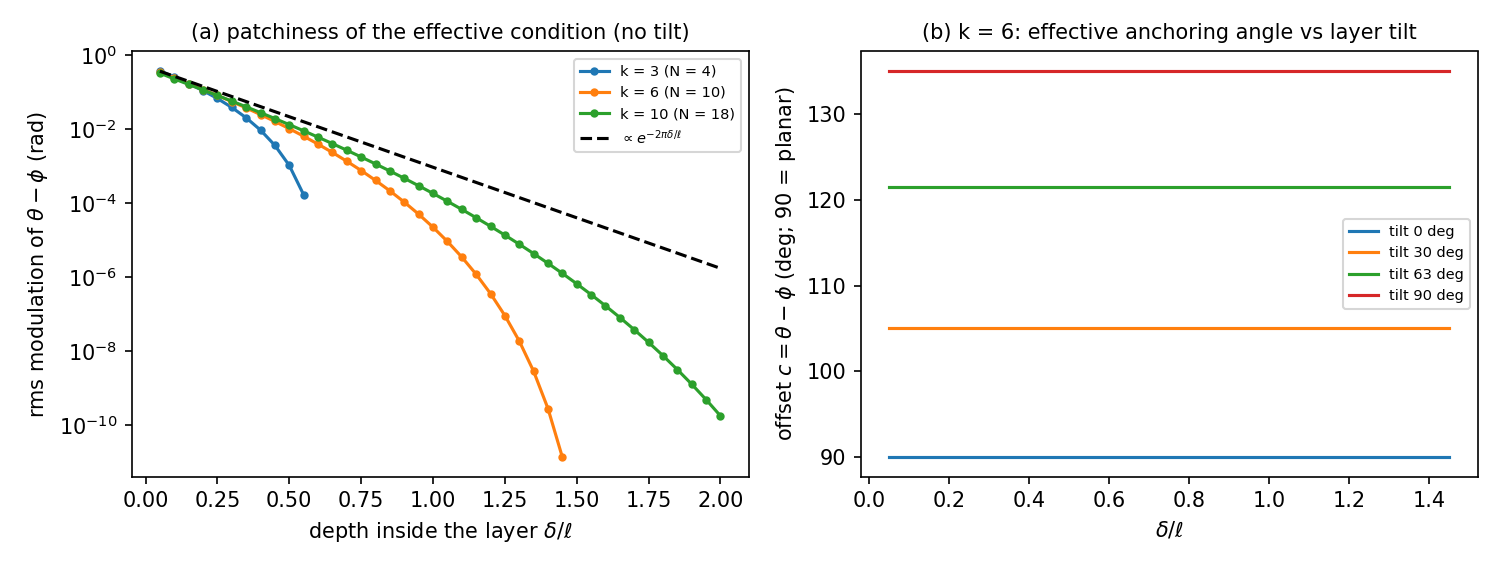
\includegraphics[width=0.9\textwidth]{effective_bc.png}
\caption{Effective boundary condition behind the wall layer (one-constant theory, $R=31.83$, central $+1$). (a) rms modulation of $\theta-\phi$ against
the depth behind the layer in units of the spacing, untilted layer, $k=3,6,10$; dashed: $e^{-2\pi\delta/\ell}$. (b) $k=6$: effective anchoring angle
$c=\theta-\phi$ (90$^\circ$ = planar) for layer tilts 0--90$^\circ$: $c=90^\circ+\tau/2$.}\label{fig:effbc}
\end{figure}
\begin{figure}[H]\centering
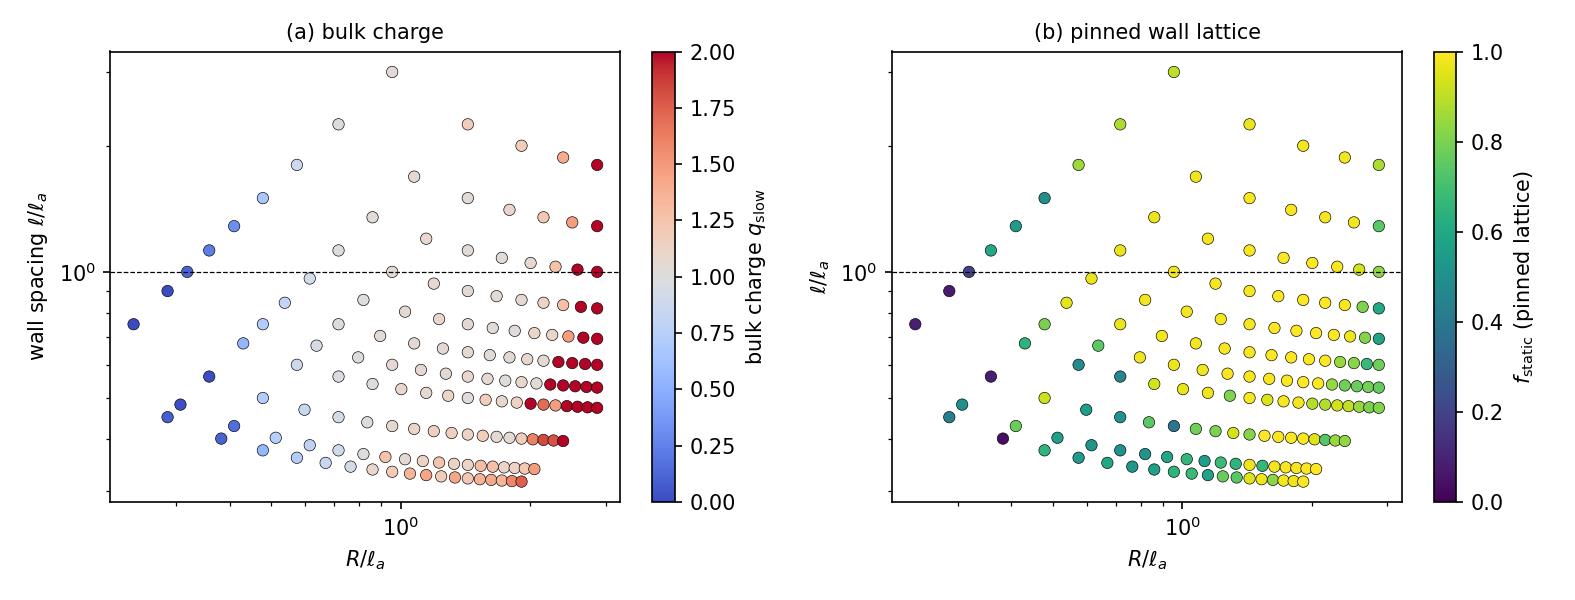
\includegraphics[width=0.9\textwidth]{spacing_criterion.png}
\caption{Main circle sweep in the plane of size $R/\ell_a$ and wall spacing $\ell/\ell_a$ (log axes; diagonals are constant $k$). (a) Bulk charge
(mobility criterion). (b) Pinned fraction of the wall lattice.}\label{fig:spacing}
\end{figure}

\subsection{A particle (defect Langevin) model: what it misses}\label{sec:defectmodel}
\emph{Idea (B.~Loewe):} each defect with its own overdamped Langevin equation, interacting elastically and as Stokeslets
(\texttt{theory/defectmodel/}). Minimal version: the $2k$ $+\half$ only (no creation or annihilation, so the observed state of $2k-2$ wall $+\half$ and a
bulk $+1$ is reachable); elastic force from the exact disk energy with images ($K=K_3$, $\mu=0.02$, thermal noise); orientation slaved to the positions
through the one-constant field (head $=-e^{2i\theta_\mathrm{rest}}$, the measured tilt lock); self-propulsion $v_0$ along the head; each $+\half$ a
point force $f$ along its head in the no-slip disk (exact Green's function, precomputed once on the unit disk, scale-free in 2D; reciprocity error 0.04\%).
Scan at $k=6$, $R=31.83$: $v_0=0.02$--0.3, $f/\eta=0$--3.
\begin{itemize}
  \item Below $v_0\approx0.1$ all 12 stay at the wall; from $v_0\approx0.15$ most leave at once (wall count 3--8): no stable $2k-2$ + $+1$ state.
  \item The circulation stays $\le0.02$ (measured 0.4--0.7) and changes sign constantly: point forces of a ring of $+\half$ largely cancel.
  \item Missing physics: the wall binding of a $+\half$ is far stronger than the log energy (orientation-dependent, the 80--110\,$k_BT$ anisotropy barrier of
        Sec.~\ref{sec:fluct}); self-propulsion is suppressed at a no-slip wall; and the circulation is driven by the distributed bulk active stress
        (Sec.~\ref{sec:dirstokes}), which a point-force model of the defects does not carry. A useful particle model needs at least an orientation-dependent
        wall potential and the $+1$ spiral stress of Sec.~\ref{sec:effbc}.
\end{itemize}

\paragraph{Adding the spiral flow to the particle model} (B.~Loewe's suggestion; \texttt{defect\_langevin.py}, \texttt{scan\_spiral.py},
\texttt{scan\_structured.py}). At every step the mean tail tilt $\tau$ of the wall defects sets the effective boundary $c=90^\circ+\tau/2$; whenever the
wall holds $2k-2$ defects (inner winding 1) the spiral body force $(\zeta/\eta)S\sin\tau/r$ ($(\zeta/\eta)S=0.48$, calibrated) acts on
$r_c<r<R-0.34\ell$ and its exact axisymmetric no-slip flow advects all defects.
\begin{itemize}
  \item \textbf{Free model} ($k=6$, $R/\ell_a=1.43$): the spiral flow matters only when the $2k-2$ + bulk $+1$ state exists. At $v_0=0.15$ this state is
        present 27--30\% of the time and the circulation then rises to 0.29--0.38 (0.007 without the spiral), but the state is not stable (wall defects still
        leave in avalanches), so the circulation flips and the tilt has no consistent sign.
  \item \textbf{Given the structure} (the $2k-2$ wall defects held radially at the layer depth, free along the wall, with the calibrated anisotropy
        pinning; the bulk pair free but kept 6 cells from the wall, because nothing in the log energy holds a $+1$ in the bulk, the passive ground state being
        $2k$ at the wall): the loop produces a circulation and a tilt that follows it. $k=6$: no circulation up to $R/\ell_a=0.6$ ($\le0.07$, tilt
        $\le10^\circ$); from 0.8, circulation 0.40, 0.65, 1.0, 1.6 at $R/\ell_a=0.8$, 1.0, 1.43, 2.0 with tilt$\times$sign(circulation) $=+24^\circ$ to
        $+29^\circ$. Without the spiral: circulation $\le0.014$, tilt $\approx5^\circ$ with no sign rule. $k=4$: onset between 0.8 and 1.0 (circulation 0.19,
        0.51, 1.07 at 0.8, 1.0, 1.43; tilt $+19^\circ$ to $+39^\circ$). The sense of rotation reverses over time, as in the simulations.
  \item Compared with the MPCD circles: circulation of the right size (0.65--1.0 against 0.6 at $R/\ell_a=1.43$), tilt smaller (30--40$^\circ$ against
        $63^\circ$), onset later ($\approx0.7$ against 0.39--0.44), and the predicted $k$-ordering (onset at larger $R/\ell_a$ for $k=4$ than for $k=6$). What keeps
        the $+1$ in the bulk, and the wall defects at the wall, remains outside the model.
\end{itemize}

\paragraph{What sets the size of the tilt: splay $\neq$ bend beyond first order} (B.~Loewe's question; \texttt{theory/aniso2/}).
In the particle model the tilt is not locked: it wanders (10--90\% range $-59^\circ$ to $+49^\circ$), the layer slips 2.4 sites per 1500 time units and the
circulation reverses often, whereas the MPCD layer sits at $\pm63^\circ$ without creep. A stable intermediate tilt needs a minimum of the tilt potential away
from zero, i.e.\ a term with a different $\tau$-dependence than the drive ($\propto\sin\tau$).
\begin{itemize}
  \item \textbf{To first order in $K_1-K_3$ this is impossible, exactly:} a registry shift rigidly adds $\tau/2$ to the one-constant director, so
        $\int(\text{splay}^2-\text{bend}^2)$ is exactly $\propto\cos\tau$ (numerically: $-66$, $-44$, $-22\,k_BT\cos\tau$ for $k=4,6,8$, all higher harmonics zero). The
        bulk $+1$ adds another $\cos\tau$ term (it prefers the pure-bend vortex: $\approx-46\,k_BT\cos\tau$ at $k=6$).
  \item \textbf{Beyond first order:} the director was relaxed under the full anisotropic Frank energy ($K_1=42$, $K_3=23.1$; correction field vanishing at the wall,
        rigid defect cores, energy outside the cores; \texttt{relax\_frank2.py}; check $K_1=K_3$: flat to a residual $0.8\,k_BT\cos2\tau$). $k=6$, $R=31.83$:
        $E(\tau)\approx-(31\text{--}47)\cos\tau+(4.6\text{--}7.6)\cos2\tau-(1\text{--}3)\cos3\tau$ $k_BT$, the sign of the $\cos2\tau$ term the same for core radius 1.5
        or 2.5, grid 0.5 or 0.35, point or paired bulk $+1$, cores fixed or free. (A first version with soft core weights failed its check and was discarded.)
  \item \textbf{This sign gives a stable tilt.} With a drive torque $D\sin\tau$, the net torque is $\sin\tau\,[D-|A_1|+4A_2\cos\tau]$: the untilted layer becomes
        unstable at $D_c=|A_1|-4A_2$ and the tilt grows continuously (supercritical) as $\cos\tau^*=(|A_1|-D)/(4A_2)$; above $D=|A_1|+4A_2$ the layer slides.
  \item \textbf{Particle model with the second harmonic} (\texttt{scan\_a2.py}; structured, $k=6$): the tilt locks where the drive is moderate. With $A_2=20\,k_BT$:
        $|\tau|=64^\circ$ (59--68$^\circ$, 99\% of the time in 45--80$^\circ$, no slip, no reversals) at $R/\ell_a=1.0$ and half the calibrated spiral drive;
        $67^\circ$ at $R/\ell_a=0.6$ with the full drive. $A_2=10$: $\approx49^\circ$; $A_2=5$ (the computed value): $\approx35^\circ$. With the full calibrated drive
        at $R/\ell_a\ge0.8$ the layer slides for every $A_2$.
  \item \textbf{Reading.} Splay $\neq$ bend supplies the missing ingredient qualitatively: a $\cos2\tau$ term of the right sign that turns the onset into a
        supercritical bifurcation with a locked finite tilt. Quantitatively the elastic estimate ($A_2\approx5$) gives $\approx35^\circ$; the measured $63^\circ$
        needs $A_2\approx15$--20, or a further contribution of the same harmonic (core energy of a tilted $+\half$ at a homeotropic wall, flow alignment). The
        calibrated drive is too strong for locking in the larger cavities, consistent with the missing brake of the wall band (Sec.~\ref{sec:dirstokes}),
        which the particle model does not contain.
\end{itemize}

\paragraph{Flow alignment} (B.~Loewe's question; \texttt{theory/flowalign/}). The MPCD nematic rotates each particle's orientation by Jeffery's rule,
$\dot{\mathbf u}=\mathbf u\cdot W+\lambda(\mathbf u\cdot D-\mathbf u\,\mathbf u\mathbf u\!:\!D)$ (Larson), with $\lambda=$ \texttt{tumble} $=2$, the rotation rate scaled
by \texttt{shearSusc} $=0.5$ (\texttt{lc.c}, \texttt{jefferysTorque}): flow aligning, Leslie angle $\tfrac12\arccos(1/\lambda)=30^\circ$ from the flow. None of the models
above contains it. Measured (active circles $R=31.83$, $k=2,6,10$, 64 snapshots each; director minus the one-constant field of the measured defects, signed by
the circulation):
\begin{itemize}
  \item \textbf{A non-elastic, flow-signed residual.} $-1^\circ$ at the wall, growing inwards to $-25^\circ$ at 6--10 cells ($k=6,10$; $-10^\circ$ at $k=2$); within 6 cells
        of the wall its size grows with the local shear ($\approx5^\circ$ at the weakest, 10--12$^\circ$ at the strongest) and its sign follows the sign of the shear.
  \item \textbf{Small at the wall layer, large in the bulk.} At the depth of the wall defects (1--2 cells) the residual is only 4--5$^\circ$: flow alignment barely rotates
        the wall defects, so it does not add tilt directly.
  \item \textbf{It erases the elastic spiral in the bulk.} The elastic field of the measured defects predicts a bulk spiral at $122$--$123^\circ$ from radial ($90^\circ+\tau/2$);
        the measured director is at $110^\circ$ 2--6 cells from the wall and $74^\circ$ ($k=6$), $87^\circ$ ($k=10$) in the bulk ($0.3$--$0.7R$): close to tangential.
  \item \textbf{Where the drive actually is.} The measured azimuthal active force (from $-\nabla\!\cdot Q$, signed by the circulation) has a net positive torque, located in a
        ring just inside the layer, $r/R\approx0.6$--0.9 (3--12 cells from the wall; the smoothing zone of the effective boundary is $\approx0.34\ell\approx6$ cells), negative
        in the wall band ($r/R>0.9$, the brake) and slightly negative in the inner bulk ($0.2$--$0.5R$). The effective-boundary drive exists but is confined to an
        annulus behind the layer; deeper in, flow alignment turns the director back towards tangential.
  \item \textbf{Consequences for the particle model.} The $1/r$ spiral force over $r_c<r<R-0.34\ell$ overestimates the drive (consistent with locking needing about half the
        calibrated drive) and puts it in the wrong place; the next version should use the measured annular drive, and flow alignment of the bulk texture.
\end{itemize}

\paragraph{Annular-drive particle model: a closure test that fails, and why} (\texttt{defectmodel/scan\_annular.py}).
The drive was replaced by the measured one: the effective azimuthal body force $f_\mathrm{eff}(r)=-(v''+v'/r-v/r^2)$ reconstructed from the measured mean swirl of the
$k=6$, $R=31.83$ circle (it agrees with $c\,\langle-\nabla\!\cdot Q\rangle_\phi$ in the driving ring, $r/R=0.7$--0.85, and has a weaker wall-band brake), scaled by
$\sin\tau/\sin63^\circ$ so that the model reproduces the measured flow exactly at the measured tilt; no defect Stokeslets (the profile contains all active forces);
structured layer, $B=90\,k_BT$, $A_2=0$--20.
\begin{itemize}
  \item \textbf{The tilt does not lock at $63^\circ$.} With the calibrated drive the median $|\tau|$ is 26--29$^\circ$ with a broad distribution, the layer slips by up to
        $130^\circ$ per 1000 time units and the circulation reverses 20--40 times; more drive gives less tilt (faster sliding), half the drive 37--55$^\circ$, still broad.
  \item \textbf{Why: in MPCD the wall defects are not carried by the flow.} The fluid at the layer depth moves at 0.13--0.16 cells per time unit (signed with the circulation),
        the wall $+\half$ at $0.0005\pm0.0010$ ($k=6$) and $0.0004\pm0.0005$ ($k=10$): an effective advection coefficient of 0.002--0.004, zero within error. The layer sits
        at a static, shifted registry ($\pm\tau/(2k-2)$ for $\pm63^\circ$); the anchored texture between the defects and the wall holds it. In the model the wall
        defects move with the fluid (0.2--0.4 cells per time unit), and the registry pinning can hold at most $\mu F\approx0.03$, so the layer slides.
  \item \textbf{Consequence.} The tilt is not produced by the flow continuously pushing the layer; it is a static state reached at the reversals. The next version
        needs the kinematics of a wall defect (a texture anchored to the wall, advection coefficient $\ll1$, to be measured from the registry jumps at reversals), after
        which the torque balance of Sec.~\ref{sec:effstab} applies with $D$ replaced by the static drag on the layer.
\end{itemize}

\subsection{Stability of the untilted layer through the effective boundary}\label{sec:effstab}
Loop (\texttt{theory/stability/effbc\_stability.py}): a registry shift $\alpha$ of the layer tilts it by $\tau=(2k-2)\alpha$ (measured lock); the bulk then sees
a spiral boundary $c=90^\circ+\tau/2$, whose extensile stress exerts $f_\phi=(\zeta/\eta)S\sin\tau/r$ in the smooth region $r_c<r<R-0.34\ell$; the axisymmetric
no-slip Stokes flow advects the layer, $\dot\alpha=v(r_s)/r_s$; the anisotropy pinning restores it at the rate $\mu E''/(Nr_s^2)$ (Sec.~\ref{sec:fluct}). Linear
growth rate $\lambda=(2k-2)(\zeta/\eta)S\,h-\mu E''/(Nr_s^2)$, $h$ the dimensionless advection of the layer per unit spiral drive (0.016--0.025).
\begin{itemize}
  \item With the calibrated $\zeta/\eta=0.42$--0.67 (director-field fit), $S=0.876$, $\mu=0.02$ and $E''$ from the anisotropy calculation, the untilted layer is
        unstable above $R/\ell_a\approx0.47$--0.50 ($k=6$), 0.4 ($k=8$), 0.6--0.75 ($k=4$), for a bulk-core radius $r_c=0.25\,\ell_a$: the size at which the measured
        circulation and tilt appear (0.39--0.44). Small cavities stay untilted because the pinning rate grows as $1/r_s^2$.
  \item The onset depends on the assumed core radius ($k=6$: 0.30--0.63 for $r_c=0$--0.4\,$\ell_a$); the robust prediction is the ordering, onset at smaller
        $R/\ell_a$ for larger $k$. The main sweep measures the onset only for $k=2$--4 (0.46, 0.39, 0.40; larger $k$ start above it), which neither confirms
        nor rejects the ordering; the defect-only tilt coherence is too noisy at small $N$. Decisive test: circulation of the small high-$k$ cavities
        ($\rho=0.16$--0.5, flows to be reduced on the server).
\end{itemize}

\subsection{Site arrangement, curvature and the second vortex}\label{sec:sitecurv}
\paragraph{Moving the pinned sites inside the circle} (B.~Loewe's idea; branch \texttt{anchmod}, \texttt{runs/anchmod\_test}). A sine-modulated winding
$\theta_\mathrm{wall}=k\phi+A\sin(m\phi)$ (eMode 2; \texttt{anchAmp}, \texttt{anchMode}, \texttt{anchPhase}; validated: $A=0$ reproduces production bit for bit, $A=1$
gives a wall director within $9^\circ$ rms of $6\phi+\sin\phi$) makes the homeotropic points, $(k-1)\phi+A\sin(m\phi)\equiv0$ (mod $\pi$), unevenly spaced while the
wall curvature and the topology stay those of the circle.
\begin{itemize}
  \item \textbf{Active (final, 9 runs, $\approx1000$ time units of production):} the wall sites sit within 0.21--0.27 cells (rms) of the predicted modulated
        homeotropic points shifted by the tilt, 2.2--4.5 cells from the best evenly spaced lattice; gaps 17--25 cells ($A=1$, $m=1$) and 14.6--30 cells ($A=1$, $m=2$);
        runs with the same sense of rotation agree within 0.06--0.13 cells whatever the initial director; opposite senses differ by 7.6 cells ($=2\tau/(2k-2)$). Tilt
        63--64$^\circ$. The anchoring pattern sets the active sites (\texttt{anchmod\_results.txt}).
  \item \textbf{Passive (3 runs): not pinned by the modulation} (my prediction was wrong). The three initial directors give site sets 3.3--8.5 cells apart. Reason: a
        modulation $A\sin(m\phi)$ couples to the ring through $\sum_je^{im\phi_j}$, which vanishes for $2k=12$ evenly spaced defects unless $m$ is a multiple of 12; $m=1,2$
        only distort the gaps (13.9--20.3 cells against 16.7 uniform) and leave the rotation free. The active ring is pinned by splay $\neq$ bend at the homeotropic points
        wherever they are; the passive one is not.
  \item \textbf{Geometry or topology: the layer does not depend on where its sites are.} Sweep with flow output (\texttt{runs/anchmod\_sweep}: $m=1$, $A=1,2,3$;
        $m=2$, $A=1,1.5,2$; 2 seeds each; random start), scored with \texttt{theory/anchmod/layer\_observables.py} against 10 uniform-circle runs: bulk charge
        0.75--0.87 (baseline 0.76--0.83), 10 wall defects in 85--97\% of the frames (88--93\%), tilt 61--63$^\circ$ with coherence 0.96--0.97 (63--64$^\circ$, 0.97), no
        reversals, no escapes (one run 0.05 per 1000 time units), circulation 0.59--0.75 (0.62--0.75), never two vortices. Moving the pinned sites by up to several cells
        leaves every property of the layer unchanged: the layer is robust to the site arrangement. The ellipse instability therefore does not come from the uneven
        arrangement of the sites but from the curvature or the elongated flow (these circles never form a second vortex, so the circle sweep alone does not separate those two;
        the ellipse analysis below does).
\end{itemize}

\paragraph{Is the second vortex what breaks the layer in ellipses?} (B.~Loewe's hypothesis; \texttt{theory/vortexlayer/}.) A single vortex asks for a uniform tilt, i.e.\
a rigid registry shift; two counter-rotating vortices ask for opposite tilts on the two halves, i.e.\ opposite shifts that compress the lattice where the vortices meet the
wall on one side and stretch it on the other, a natural source of vacancies and escapes. Test on the active ellipses (W3, two seeds): per flow interval, one or two
vortices; escapes = wall $+\half$ followed for 20 time units (nearest-neighbour chains) that end deeper than 6 cells (a first version counting single-frame escapes had too
few events and was discarded).
\begin{table}[H]\centering\small
\caption{Escape probability of a wall $+\half$ within 20 time units, and mean number of vacancies, in one- and two-vortex intervals (1500--2700 escapes per state at
$\varepsilon\ge1.5$). Meeting region: $|x|<A/4$, where the two vortices meet the wall; tips: $|x|>A/2$.}\label{tab:vortexlayer}
\begin{tabular}{lccccc}\toprule
& state & escape prob. & meeting region & tips & vacancies\\\midrule
$\varepsilon=1.2$ & one vortex (always) & 0.005 & 0.004 & 0.006 & 0.22\\
$\varepsilon=1.5$ & one vortex & 0.072 & 0.038 & 0.104 & 2.31\\
 & two vortices & 0.066 & 0.049 & 0.080 & 2.31\\
$\varepsilon=2.0$ & one vortex & 0.070 & 0.066 & 0.081 & 2.70\\
 & two vortices & 0.077 & 0.076 & 0.093 & 2.73\\\bottomrule
\end{tabular}
\end{table}
\begin{itemize}
  \item \textbf{No instantaneous link.} At $\varepsilon\ge1.5$ the layer is $\approx14\times$ leakier than at $\varepsilon=1.2$ in both vortex states; vacancies are the same; the
        two-vortex indicator and the escape rate are uncorrelated at lags from $-200$ to $+200$ time units ($|r|\le0.11$).
  \item \textbf{Escapes concentrate at the tips}, not where two vortices meet the wall.
  \item \textbf{Reading.} Elongation, most likely the tip curvature, weakens the layer at all times and also allows the second vortex: two consequences of the geometry rather
        than cause and effect. Caveat: the vortex state switches every few hundred time units, and slow healing could hide a time-integrated effect. The circle sweep above
        (uneven sites, no tips) separates the two: an intact circle layer would point to curvature, a leaking one to the site arrangement.
\end{itemize}

\subsection{Response of the wall layer to an imposed vortex and its reversal}\label{sec:swirl}
(B.~Loewe's suggestion; \texttt{theory/reversals/swirl\_response.py}.) An optional azimuthal body acceleration was added to the solver (branch \texttt{anchmod},
\texttt{bin/mpcd\_swirl.out}; inputs \texttt{swirlAcc}, \texttt{swirlRadius}, \texttt{swirlX/Y}, \texttt{swirlFlipTime}, \texttt{swirlPeriod}; production steps only;
switched off it reproduces production bit for bit). Runs: $k=6$, $R=31.83$, acceleration within $0.6R$ (away from the layer), reversed at production time 1500.
\begin{table}[H]\centering\small
\caption{Imposed swirl and its reversal. Circulation and tilt before $\to$ after; times of their zero crossings after the reversal; registry shift of the layer
(measured, and predicted by the tilt lock $\Delta\tau R_l/N$).}\label{tab:swirl}
\begin{adjustbox}{max width=\textwidth}
\begin{tabular}{lcccccc}\toprule
run & circulation & fluid at layer & tilt (deg) & $t_0$ circ., tilt & registry shift (lock) & transit\\\midrule
active, $A=0.005$ & $+0.79\to+0.40$ & $+0.16\to+0.06$ & $+64\to+64$ & not reversed & $-0.1$ ($0$) & --\\
active, $A=0.01$ & $+0.97\to-0.93$ & $+0.16\to-0.17$ & $+65\to-65$ & 375, 678 & $-7.2$ ($-6.8$) & 344, from $+448$\\
active, $A=0.02$ & $+1.13\to-1.15$ & $+0.16\to-0.16$ & $+66\to-66$ & 295, 384 & $-7.3$ ($-7.0$) & 42, from $+380$\\
passive, $A=0.003$ & $+0.18\to-0.18$ & $+0.02\to-0.02$ & $+57\to-57$ & 115, 236 & $+4.4$ (slides) & --\\
passive, $A=0.01$ & $+0.49\to-0.49$ & $+0.06\to-0.06$ & $+63\to-59$ & 105, 210 & $+40$ (slides) & --\\
passive, $A=0.02$ & $+0.74\to-0.74$ & $+0.09\to-0.09$ & $+68\to-66$ & 85, 164 & $+44$ (slides) & --\\\bottomrule
\end{tabular}
\end{adjustbox}
\end{table}
\begin{itemize}
  \item \textbf{The active vortex resists a weak reversal} ($A=0.005$: circulation reduced but not reversed, tilt unchanged): the self-sustained state is bistable.
  \item \textbf{The active layer is a stick--slip system.} It stays at its registry until the flow at its depth has reversed, then jumps by the amount the lock predicts
        ($-7.2$, $-7.3$ cells against $-6.8$, $-7.0$) within 42--344 time units, and locks at the mirror registry. The tilt lags the circulation by 90 time units at the
        stronger drive, as at the spontaneous reversals of circles (Sec.~\ref{sec:hydro}). The near-zero advection in the steady state (Sec.~\ref{sec:effstab}) is
        pinning, not insensitivity to the flow.
  \item \textbf{A passive layer under imposed flow tilts too, to $\pm57$--$68^\circ$}, nearly independent of the flow strength (fluid at the layer 0.02--0.09), and
        slides with the flow (40--44 cells; the passive ring is not pinned). In the active cavities the tilt is an active effect (the only flow there is the active
        flow), but its \emph{angle} appears to be set by the response of the wall layer to the presence of flow.
  \item \textbf{The angle is controlled by the flow-alignment parameter} (\texttt{runs/swirl\_tumble}, passive, imposed swirl, \texttt{tumble} $\lambda$ changed): final tilt
        $\approx28$--$36^\circ$ at $\lambda=0.5$ (tumbling), 57--65$^\circ$ at $\lambda=1.2$ (43$^\circ$ after the reversal at the stronger drive), 57--68$^\circ$ at $\lambda=2$,
        75--83$^\circ$ at $\lambda=4$. The tilt grows monotonically with $\lambda$, so it is set by the flow alignment of the nematic at the wall; the simple guess
        $2\theta_L=\arccos(1/\lambda)$ (34$^\circ$, 60$^\circ$, 76$^\circ$) fails at $\lambda=1.2$, and the tumbling case still tilts, so the agreement at $\lambda=2$, 4 is not
        evidence for it. The active runs all use $\lambda=2$.
\end{itemize}
\begin{figure}[H]\centering
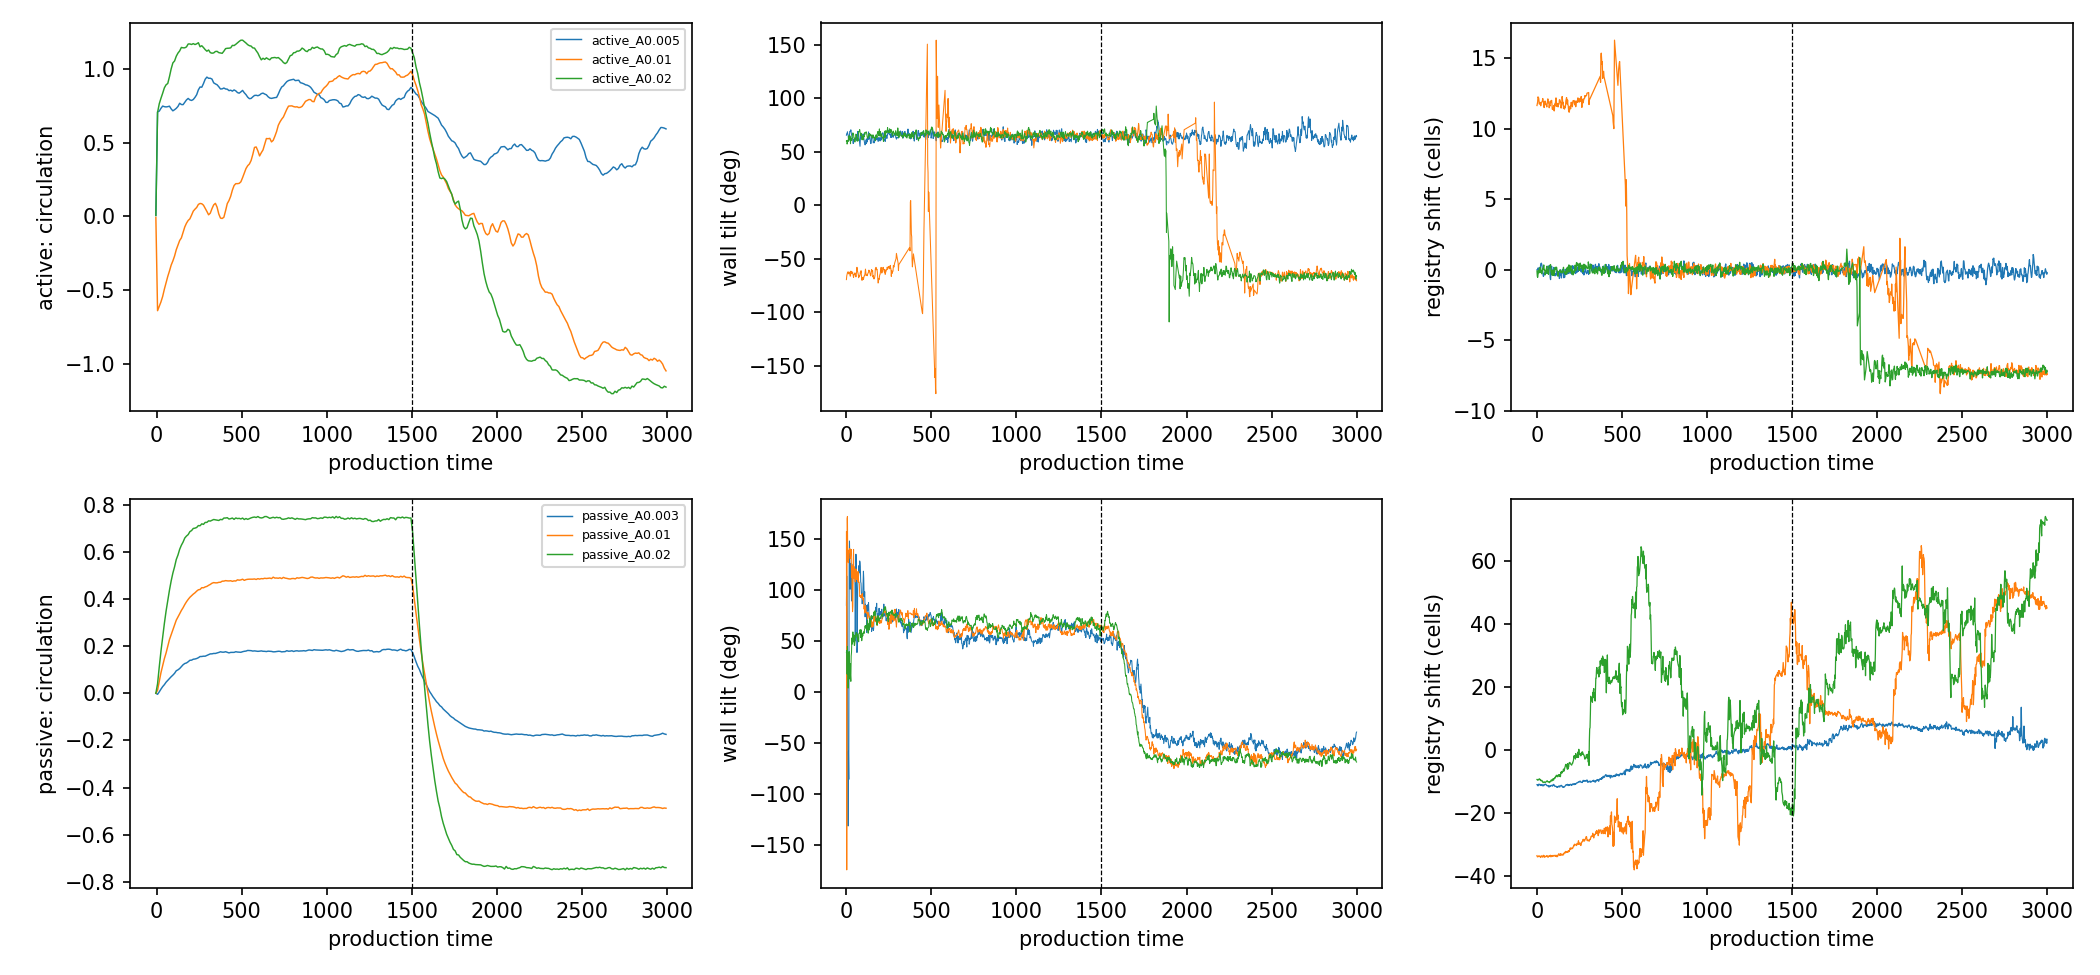
\includegraphics[width=\textwidth]{swirl_response.png}
\caption{Imposed swirl reversed at production time 1500 (dashed). Top: active; bottom: passive. Circulation, wall tilt and registry shift of the layer.}\label{fig:swirl}
\end{figure}

\subsection{Half-integer windings}\label{sec:halfk}
A nematic allows half-integer $k$: the wall director $k\phi$ returns to itself up to a sign after one turn, and the code's anchoring is insensitive to that sign
(the particle orientation is projected on the imposed director). The pattern then has an odd number, $2k-2$, of homeotropic points and no inversion symmetry.
Runs: $k=0.5$, 1.5, 2.5, 3.5, 5.5, $R=31.83$, active (2 seeds) and passive (1), production binary (\texttt{runs/halfk}; \texttt{theory/halfk/analyse\_halfk.py}).
\begin{itemize}
  \item \textbf{$k\ge2.5$ behaves exactly like integer $k$.} Active: $2k-2=3$, 5, 9 wall $+\half$ in 85--93\% of the frames; registry on the odd set of homeotropic
        points (lock-corrected $D=0.00\pm0.09$, concentration 0.99--1.00); tilt 63--65$^\circ$, coherence 1.00; bulk charge as for integer $k$; one steady vortex
        (circulation 0.66--0.74, no reversals). The integer references ($k=2$--6, same $R$): 2--10 wall defects, tilt 59--65$^\circ$, circulation 0.62--0.74. An odd
        number of sites and the missing inversion symmetry change nothing.
  \item \textbf{$k=1.5$ (one wall site predicted): no layer.} The wall stays empty (0.04 wall $+\half$ on average); the charge $3/2$ sits in the bulk (about three $+\half$,
        bulk charge $\approx1.25$); the flow is weak and erratic (circulation 0.08--0.12, 6--7 reversals). One defect cannot make a smooth effective boundary (its smoothing
        depth, $\approx2R$, exceeds the radius; Sec.~\ref{sec:effbc}). $k=2$ (two sites, smoothing depth $\approx R$) still forms its layer.
  \item \textbf{$k=0.5$:} no layer; a single $+\half$ circulates in the bulk at $\approx0.6R$ and drives a strong, steady vortex (0.42--0.49, at most one reversal).
  \item \textbf{Passive:} consistent with the depth law. At $k=0.5$ the single $+\half$ sits near the centre (the law gives $r^*=0$); for $k=1.5$--3.5 the predicted ring is
        deep (6.7--2.6 cells) and straddles the 4-cell wall band; at $k=5.5$ all 11 sit at the wall with the frustrated tilt pattern of a $2k$ ring.
\end{itemize}

\subsection{Flow-induced ejection: why the active wall holds $2k-2$}\label{sec:ejection}
\emph{Mechanism (B.~Loewe):} the vortex means flow; flow tilts the wall defects; the tilted $2k$ ring becomes too expensive and two defects leave.
\paragraph{Energetics} (\texttt{theory/ejection/}; rigid cores of radius $a$, director relaxed outside them; one-constant $K=32.5$ and anisotropic $K_1=42$,
$K_3=23.1$; $k=4,6,8$, $R=31.83$). A: the $2k$ ring. B: a $2k-2$ ring (bulk charge 1) plus two $+\half$ at $\pm0.45R$; both contain the same $2k$ defects, so core
energies cancel. Flow alignment is modelled by forcing every wall core to the same tilt $\tau$. Validation: unrelaxed, one-constant, $\tau=0$ with natural cores,
$E_B-E_A=+183.7\,k_BT$ numerically against $+184.0$ from the image formula.
\begin{itemize}
  \item \textbf{Without flow the $2k$ ring is stable:} ejecting two defects costs $+155$ to $+200\,k_BT$ (all $k$, both elasticities, $a=1.5$, 2.5).
  \item \textbf{A common tilt frustrates the $2k$ ring.} Its natural tilts wind around it ($150^\circ,90^\circ,30^\circ,\dots$ at $k=6$; Sec.~\ref{sec:status}); forcing them
        equal costs $+375$ to $+475\,k_BT$ at $k=6$ ($+200$ to $+510$ for $k=4$--8), nearly independent of the value of $\tau$. The $2k-2$ ring takes a common tilt by a registry shift, almost for free
        ($<40\,k_BT$).
  \item \textbf{Under a common tilt the ejected structure is cheaper} by 20--330\,$k_BT$, for every $k$, both elasticities and both core sizes (the magnitude depends on
        the core size, the sign does not).
\end{itemize}
\paragraph{Direct test: passive cavities under imposed flow eject two defects.} In the passive imposed-swirl runs (Sec.~\ref{sec:swirl}; no activity) the wall goes
from 12 to 10 $+\half$ and the bulk acquires charge $+1$: $\lambda=2$, $A=0.003$: $12\to11\to10$ (bulk $0\to0.5\to0.8$); $A=0.01$, 0.02: $12\to10$ (bulk $\to0.9$--1.0);
$\lambda=4$, both $A$: $12\to10$ (bulk 1.0). $\lambda=1.2$: only partly, at the stronger drive ($12\to11$, bulk 0.5); $\lambda=0.5$ (tumbling, no aligned angle): never.
The tilts measured in those runs ($\pm57$--$83^\circ$) are those of the 10-defect ring left after the ejection.
\paragraph{Reading.} The structure of the active cavities, $2k-2$ wall $+\half$ and a bulk $+1$, follows from flow plus flow alignment: flow imposes a common tilt on the
wall defects, a $2k$ ring cannot take a common tilt (its tilts must wind), so two defects leave into the bulk, leaving the largest ring that can tilt uniformly. Activity
enters by providing the flow. This links the onset of the bulk charge to the onset of a coherent flow, and predicts that a nematic with a smaller flow-alignment parameter
holds more defects at the wall under the same flow.
\begin{figure}[H]\centering
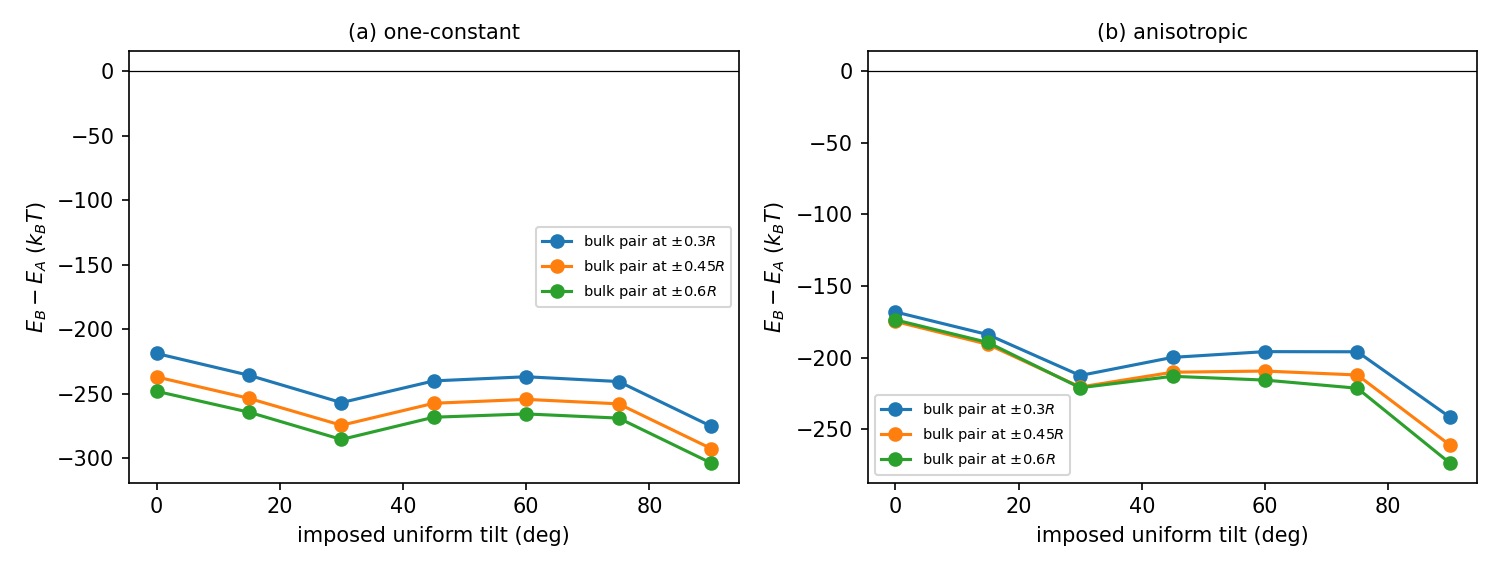
\includegraphics[width=0.9\textwidth]{tilted_structures.png}
\caption{Energy of the ejected structure (B: $2k-2$ ring plus a bulk pair) minus the $2k$ ring (A), both with every wall core forced to the same tilt, $k=6$,
$R=31.83$, for three positions of the bulk pair; (a) one-constant, (b) anisotropic. Negative: ejection favoured. (Baseline without forcing, natural tilts:
$E_B-E_A\approx+180\,k_BT$.)}\label{fig:ejection}
\end{figure}

\subsection{Ejection threshold and the negative layer}\label{sec:ejection2}
\begin{itemize}
  \item \textbf{Threshold} (\texttt{runs/swirl\_threshold}; passive circle $k=6$, $R=31.83$, constant swirl, 2 seeds; \texttt{theory/overnight/}): no ejection up to $A=0.003$ in
        3000 time units (wall 12, tilt coherence 0.2--0.5, circulation/$v_\mathrm{rms}$ up to 0.77); at $A=0.01$ both seeds eject two (wall 10, bulk $+0.75$, $+0.93$) and the tilt
        coherence jumps to 0.90--0.96. The ejection needs a flow strong enough to impose a common tilt; a reversal helps (the reversed $A=0.003$ run of
        Sec.~\ref{sec:swirl} ejected).
  \item \textbf{Negative layer} ($k=-6$, $R=28.21$, passive, imposed swirl; \texttt{theory/ejection/ejection\_neg.py}). Energetics: the commensurate 14-ring
        ($2|k-1|$) has uniform natural tilts ($\pm60^\circ$: one arm into the bulk), the 12-ring's wind; under a common tilt the 14-ring plus a bulk $+1$ is cheaper by
        196--392\,$k_BT$ minus the core cost of a created $\pm\half$ pair. Simulation: the wall stays at 12 $-\half$ for $\lambda=0.5$, 2; only $\lambda=4$ reaches 13. Gaining
        $-\half$ needs pair creation in the bulk, rare without activity: kinetically blocked, not refuted. A fair test needs activity or a seeded pair.
\end{itemize}

\subsection{Shapes: the sweep through the circle framework}\label{sec:shapesweep}
Server sweep (675 runs: Cassini ovals $b/a=1.1$--3.0, ellipses $\varepsilon=1.2$--2.5, circles; $R_\mathrm{eq}=1.0$, 1.5, 2.0\,$\ell_a$; five densities; 3 seeds;
\texttt{theory/shapes/}).
\begin{itemize}
  \item \textbf{One transition, set by the aspect ratio alone.} Tilt coherence, circulation and the single-vortex state collapse together at aspect 1.25--1.37, for ellipses and
        ovals at every size (Fig.~\ref{fig:phaseshapes}); the long semi-axis at the transition ranges from 1.2 to 2.3\,$\ell_a$, so no length sets it. Below it the cavity behaves
        like a circle (no vacancies, bulk $\approx+1$, coherence 0.92--0.94, one vortex); above it vacancies 1.5--2.9, bulk charge 1.4--2.0, coherence 0.39--0.63, circulation
        0.04--0.30, two vortices 32--84\% of the time, escapes 15--20$\times$.
  \item \textbf{Above it the layer loses more with size}: about 1, 3 and 4.5 vacancies at $R_\mathrm{eq}=1.0$, 1.5, 2.0\,$\ell_a$ (bulk charge 1.1, 1.8, 2.5).
  \item \textbf{The local lock survives everywhere} (0.91--0.97): what fails is the occupancy of the layer and the coherence of the flow.
  \item \textbf{Escapes} (pooled, by local wall curvature): rise at $\kappa R_\mathrm{eq}\gtrsim1.25$, but non-circular cavities leak 5--10$\times$ more than circles even at
        circle-like curvature: part global, part local.
  \item \textbf{Tips.} Measured effective potential of wall $+\half$ ($-\ln P(\text{depth})$, in units of the active noise; same noise at tips and flanks checked): wells
        25--35\% shallower at the tips at $\varepsilon\ge1.5$, consistent with the 2--2.5$\times$ faster escapes there; not set by the vortex number; not explained by static
        elasticity ($\approx8\%$) nor by a tilt misfit (the local lock holds at every site). With lock-produced tilts, one vortex weakens the tips by 1--2\,$k_BT$ and two vortices
        weaken the flanks (their meeting points) by 3--4\,$k_BT$, as observed at the flanks; the tip weakness in two-vortex intervals remains unexplained.
\end{itemize}
\paragraph{Is the deficit caused by the loss of coherent flow? Not settled.}
\begin{itemize}
  \item \emph{Passive ellipses with an imposed single vortex} (\texttt{runs/swirl\_ellipse}): at $\varepsilon=1.5$ the wall goes 12$\to$10, the bulk gains $+1$, the tilt becomes
        coherent: with a coherent flow an ellipse behaves like a circle; curvature alone does not prevent the $2k-2$ layer.
  \item \emph{Active ellipses with an imposed vortex}: the layer is not repaired (wall 7--8, bulk 1.5--1.7, two vortices 36--56\% of the time) even when the imposed swirl brings
        the circulation to 0.57--0.66\,$v_\mathrm{rms}$.
  \item \emph{Per interval} (450 elongated runs, 22\,500 intervals): the wall count does not follow the instantaneous flow ($|r|\le0.05$ with the circulation, $\le0.15$ with the
        tilt coherence, any lag; same vacancies with one or two vortices). In circle-like cavities it does ($r=+0.25$).
  \item \textbf{Not decisive.} The imposed vortex never made the active ellipses circle-like coherent (tilt coherence 0.62--0.64 against 0.97 in circles; two vortices still
        36--40\% of the time), so activity disrupting the coherent flow (B.~Loewe) remains a viable explanation of the deficit; the interval correlations argue against it only
        weakly, since elongated cavities may never reach circle-like coherence. Tests running: stronger imposed vortices (swirl 0.06, 0.1) in active ellipses, and vacancies binned
        by tilt coherence. Alternatives: escape/refill kinetics at the curved tips; the bulk defect population.
\end{itemize}
\begin{figure}[H]\centering
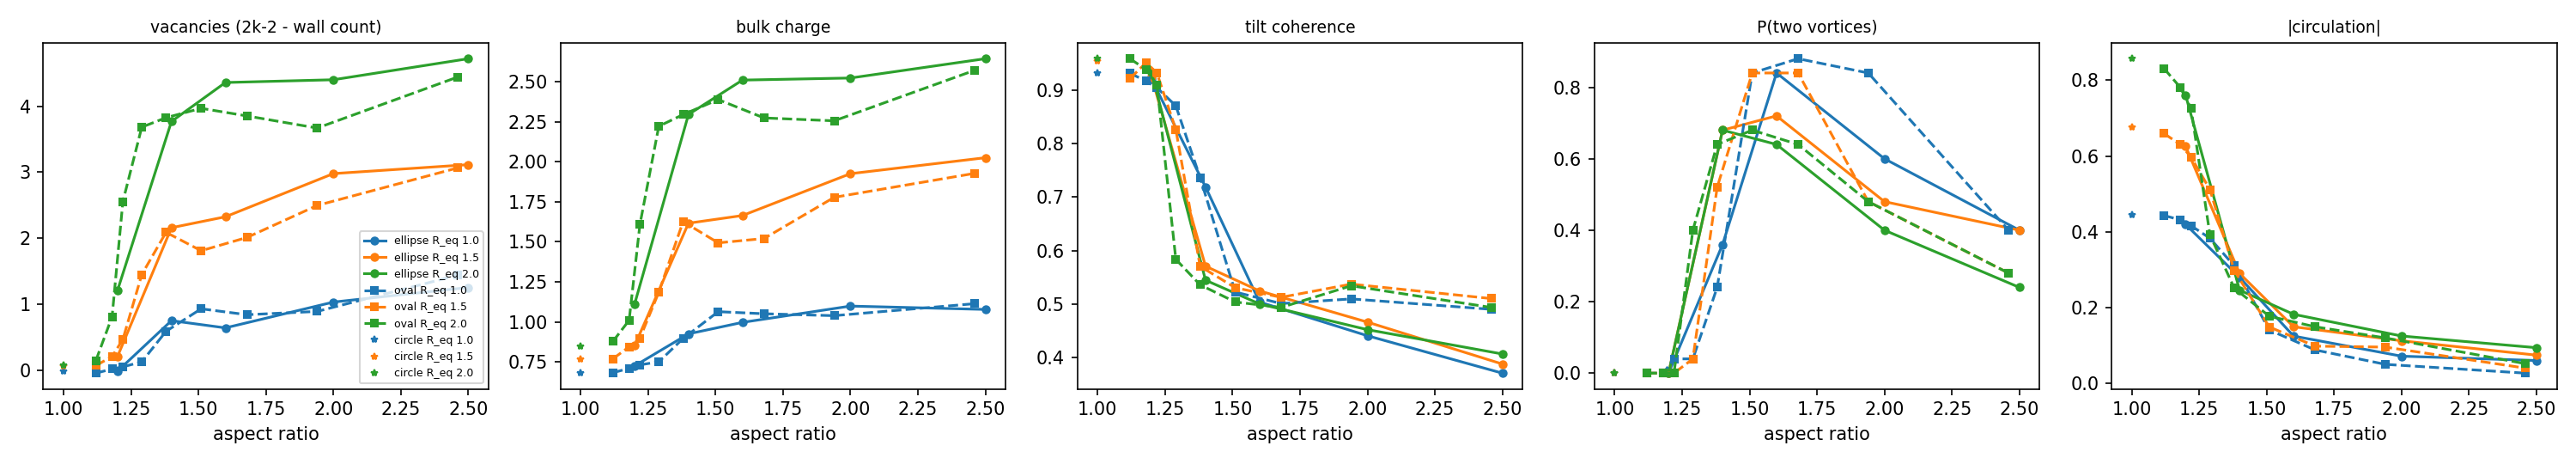
\includegraphics[width=\textwidth]{phase_shapes.png}
\caption{Shape sweep: vacancies, bulk charge, tilt coherence, probability of two vortices and circulation against the aspect ratio, for ellipses (solid) and ovals (dashed) at
$R_\mathrm{eq}=1.0$, 1.5, 2.0\,$\ell_a$ (colours); stars: circles. Medians over $k$, densities and seeds.}\label{fig:phaseshapes}
\end{figure}


\subsection{The tilt angle: flat no-slip wall in shear}\label{sec:tiltangle}
(\texttt{theory/shear\_tilt/}: \texttt{flatwall.py}, \texttt{flatwall\_scan.py}, \texttt{mpcd\_profile.py}, \texttt{solvability.py}.) Question (B.~Loewe): does the no-slip shear set the
tilt, and can its value ($\approx62^\circ$) be computed? Local limit: a flat wall at $y=0$, simple shear $v_x=sy$ (no slip), periodic along the wall with one site spacing $a_s$.
\paragraph{Equations.} Director angle $\theta(x,y)$ from the wall direction; anchoring $\theta(x,0)=\pi/2+qx$, $q=\pi/a_s$ (homeotropic at $x=0$, a rotation by $\pi$ per
period, screened by one $+\half$ at depth $d$). One-constant Ericksen--Leslie in the director limit,
\begin{equation}
\gamma_1(\partial_t+\mathbf v\cdot\nabla)\theta = K\nabla^2\theta+\gamma_1\frac{s}{2}\left(\lambda\cos2\theta-1\right),\label{eq:el}
\end{equation}
($-s/2$: rotation with the vorticity; $\lambda\frac s2\cos2\theta$: strain alignment; aligned angle $\cos2\theta_L=1/\lambda$, stable for $\lambda>1$).
\paragraph{Step 1: the layer is a zero mode.} At $s=0$, $\theta$ is harmonic. If $\theta_0(x,y)$ is a solution with the defect at $x=0$, then
$\theta_D(x,y)=\theta_0(x-D,y)+qD$ satisfies the same anchoring ($\theta_w(x-D)+qD=\theta_w(x)$) and has the same energy $\frac K2\int|\nabla\theta|^2$: a one-parameter
family. Translating the defect by $D$ rotates the far field by $\theta_\infty=qD$, and near the core ($\theta\simeq\frac12\arg(z-z_D)+c_D$, $c_D=c_0+qD$) rotates the comet axis
by $2qD$. Hence $\tau=2\theta_\infty=2\pi D/a_s$: the tilt--position lock (Sec.~\ref{sec:status}) is this zero mode.
\paragraph{Step 2: leading order.} Beyond the screening length $a_s/2\pi$ the texture is uniform along $x$ (corrections $\propto e^{-2\pi y/a_s}$) and \eqref{eq:el} reduces
to $K\theta''=-\gamma_1\frac s2(\lambda\cos2\theta-1)$. Its only bounded stable state is $\theta=\theta_L$. If the near-wall region transmits no torque, the outer
region is uniformly aligned, the layer sits on the zero mode with $\theta_\infty=\theta_L$, and
\begin{equation}
\tau_0=2\theta_L=\arccos(1/\lambda),
\end{equation}
independent of $s$, $K$ and $\gamma_1$ (the angle is set by the ratio of strain to vorticity in simple shear, which the no-slip wall fixes).
\paragraph{Step 3: boundary-layer correction.} Linearising the outer problem about $\theta_L$, $\theta=\theta_L+\delta$:
$K\delta''=\gamma_1 s\sqrt{\lambda^2-1}\,\delta$, so $\delta=\delta_0e^{-y/\ell_E}$ with the alignment length $\ell_E=\sqrt{K/(\gamma_1 s\sqrt{\lambda^2-1})}$. A torque $\Gamma$ per
unit length passed from the near-wall region gives $K\delta'=-\Gamma$, i.e.\ $\delta_0=\Gamma\ell_E/K$. \emph{Ansatz:} in the band $0<y<d$ between the wall and the defects the
director follows the winding anchoring ($\langle\cos2\theta\rangle\approx0$ over a period), so its alignment torque averages out and only the vorticity acts,
$\Gamma=\gamma_1 sd/2$, transmitted in full to the layer (the band moves with the zero mode). Then
\begin{equation}
\tau=\arccos\frac1\lambda+d\sqrt{\frac{\gamma_1 s}{K}}\,(\lambda^2-1)^{-1/4}.\label{eq:tilt}
\end{equation}
The correction grows as $\sqrt s$ (weak dependence on the flow strength) and diverges towards tumbling ($\lambda\to1$).
\paragraph{Tests.} (i) Flat-wall Q-tensor simulation ($L=a=\Gamma=1$, so $K/\gamma_1=1$): far field $2\theta_\infty=2\theta_L$ within $1^\circ$;
registry$\times360^\circ$ = tilt (zero mode); $s\to0$: $\tau\to\arccos(1/\lambda)$ (61.8 vs $60^\circ$ at $\lambda=2$, 49.5/48.2 at 1.5, 76.9/75.5 at 4). Eq.~\eqref{eq:tilt} with the
measured depth, no free parameter, over 35 runs ($\lambda=1.1$--4, $s=10^{-3}$--$10^{-1}$, $a_s=10$--40): measured/predicted correction 0.97 (median), correlation 0.98.
(ii) Removing the shear from the band next to the wall (rigid rotation there, the wall slips) raises the tilt by $\approx30^\circ$ (disk model), as the vorticity term of the ansatz implies.
\paragraph{Caveat: crowded layers tilt less (2026-10-15, open).} The law has no wall-density dependence, and the $\lambda$ scan tests it only in sparse layers
($\rho=k/\pi R\approx0.045$--0.09). In the main circle sweep ($\lambda=2$, $0.8\le R/\la\le2.2$) the tilt of the coherent layer ($C>0.9$, 10 seeds) falls steadily with $\rho$: 64.6$^\circ$
($\rho\approx0.04$), 63.0$^\circ$ (0.065), 54.7$^\circ$ (0.10), 44.2$^\circ$ (0.14; spacings down to $\lesssim17$ cells), while the flat-wall model shows no spacing
dependence for $a_s=10$--40. To check with the 10-seed sweep: tilt vs coherence, $|\langle v_\theta\rangle|$ and wall count (neighbour interactions vs weaker shear vs
measurement noise). The clean trend suggests a derivable correction. \textbf{First check (10 seeds, \texttt{theory/tiltcrowd/tilt\_crowding.py, plot\_tilt\_k.py}):} the drop is real, not a measurement effect. In frames where the layer is fully coherent
($C>0.9$) the tilt still falls from $64.6^\circ$ ($\rho\approx0.04$) to $44^\circ$ ($\rho\approx0.14$), and defects at the mean spacing drop as much as the layer.
The tilt collapses on the wall-defect spacing $2\pi R/(2k-2)$ (residual 1.7$^\circ$ against a raw spread of 7$^\circ$; $k$ or $R$ alone leave 5--6$^\circ$):
$\approx64^\circ$ for spacings $\gtrsim20$ cells, $60^\circ$ at $\approx15$, $\approx42^\circ$ at 7 cells; small cavities sit slightly below at equal spacing. TODO: does the smaller tilt help denser windings hold their layers (released fraction 0.61 at
$q=0.02$, 0.10 at $q=0.07$)? Tension: escapers untilt first, so a smaller tilt alone should favour escape.

\paragraph{Status of the derivation.} Steps 1--2 and the boundary-layer form of step 3 are derived. The transmitted torque $\gamma_1sd/2$ is an ansatz confirmed numerically
but not derived: projecting the full torque density onto the zero mode over the static texture (\texttt{solvability.py}) does not reproduce it (wrong sign once advection is
included, wrong $\lambda$ dependence); the projection is dominated by the region next to the core, where the fixed-$S$ director description fails. Open.
\paragraph{Mapping to MPCD.} MPCD rotates each particle by Jeffery's equation with Bretherton parameter $\lambda$ (\texttt{larsonRotRate}); \texttt{shearSusc} multiplies vorticity
and strain alike, so it changes the rate, not the angle. For $\dot\psi=-\frac s2(1-\lambda\cos2\psi)$, the moment $\langle e^{2i\psi}\rangle=S_2e^{2i\theta}$ obeys
$\dot\theta=-\frac s2\left[1-\lambda\frac{1+S_4}{2S_2}\cos2\theta\right]$, so $\lambda_\mathrm{eff}=\lambda(1+S_4)/(2S_2)$; with a Maier--Saupe distribution at the measured
$S_2=0.83$--0.88, $\lambda_\mathrm{eff}=1.80$--1.83 ($\lambda=2$), 3.61--3.66 ($\lambda=4$), 1.08 ($\lambda=1.2$). Leading order: 56--57$^\circ$, $74^\circ$, $23^\circ$.
Measured in the passive swirl runs: the tilt equals twice the director angle at the defects' depth (65.5 and 61.6 against 63.7 and 61.0$^\circ$, $\lambda=2$), with the director in the layer
at 26--33$^\circ$ against $\theta_L=28^\circ$. Matching the measured 61--64$^\circ$ with Eq.~\eqref{eq:tilt} ($d=1.75$, $s=0.047$) needs $\gamma_1/K=0.07$--0.18; then $\lambda=4$ gives
77--79$^\circ$ (measured 83) and $\lambda=1.2$ gives 32--37$^\circ$ (measured 57, weakly coherent, near tumbling). An independent MPCD measurement of $\gamma_1$ would make this a prediction.
\paragraph{Active continuum model (2026-10-09).} Q-tensor with Stokes flow, backflow and an extensile active stress $-\zeta Q$ (\texttt{shear\_tilt/active\_bf.py},
\texttt{scan\_active2.py}; one constant, no imposed flow, started from the passive 12-ring, $k=6$, $R=31.83$): $\zeta=0.1$: a vortex (circulation 0.92), no ejection (tilt coherence
0.47); $\zeta=0.3$, 1.0 at $\lambda=2$: vortex, ejection 12$\to$10 with bulk $+1$, coherent tilt 61.7, 62.1$^\circ$ (MPCD active $\approx62^\circ$), independent of $\zeta$; $\lambda=4$:
76.5$^\circ$; $\lambda=1.2$: 37.1$^\circ$. Passive with backflow and an azimuthal body force: ejection, 65.5--65.8$^\circ$ ($\lambda=2$), 77.6$^\circ$ ($\lambda=4$). The full chain
self-organises in a continuum active nematic. (A first attempt with $\zeta\le0.03$ developed no flow.) Free $\pm\half$ mobility in the bulk from pair annihilation
(\texttt{runs/rotvisc/quench\_L96}, \texttt{theory/mobility/}): $r^2$ linear in time to annihilation, $\mu\approx0.0054$, $4\times$ below the wall-defect value 0.02.

\paragraph{Correction (2026-10-09, evening): the MPCD tilt does not follow $\lambda_\mathrm{eff}$.} Particle-level moments (\texttt{runs/tiltdiag}, \texttt{trajOut}) confirm the
Maier--Saupe $S_4$ (within 0.01 in bulk and layer; slightly higher in the cores, $\lambda_\mathrm{eff}=1.98$--2.01 there). But varying the order with the mean-field potential gives a tilt
nearly independent of it: 62.2$^\circ$ ($U=5$, bulk order 0.56), 61.5--62.4$^\circ$ ($U=10$, 0.87; also at density 10), 64.8$^\circ$ ($U=20$, 0.94), against $\lambda_\mathrm{eff}$
predictions of 61.5/56.7/58.2$^\circ$ (bulk order) and 68.5/58.7/57.2$^\circ$ (order near the cores). The data follow the bare $\arccos(1/\lambda)=60^\circ$ plus 2--5$^\circ$; the
order-near-the-cores contribution proposed above is withdrawn, and the remaining degrees are attributed to splay $\neq$ bend ($+2$--3$^\circ$ in the disk model) and the boundary layer.
Why the particle-averaged alignment does not appear in MPCD is open (\texttt{theory/tiltdiag/}). Density 40 per cell: 62.6$^\circ$ (density has no effect). Rotational viscosity, final (4 seeds, modes $m=2$--4): $\gamma_1\approx60$ (splay $62\pm2$, bend $56\pm2$), consistent with the free-defect mobility 0.0054; the boundary-layer ansatz would then add $\approx16^\circ$ in MPCD against the measured 2--5$^\circ$.

\begin{figure}[H]\centering
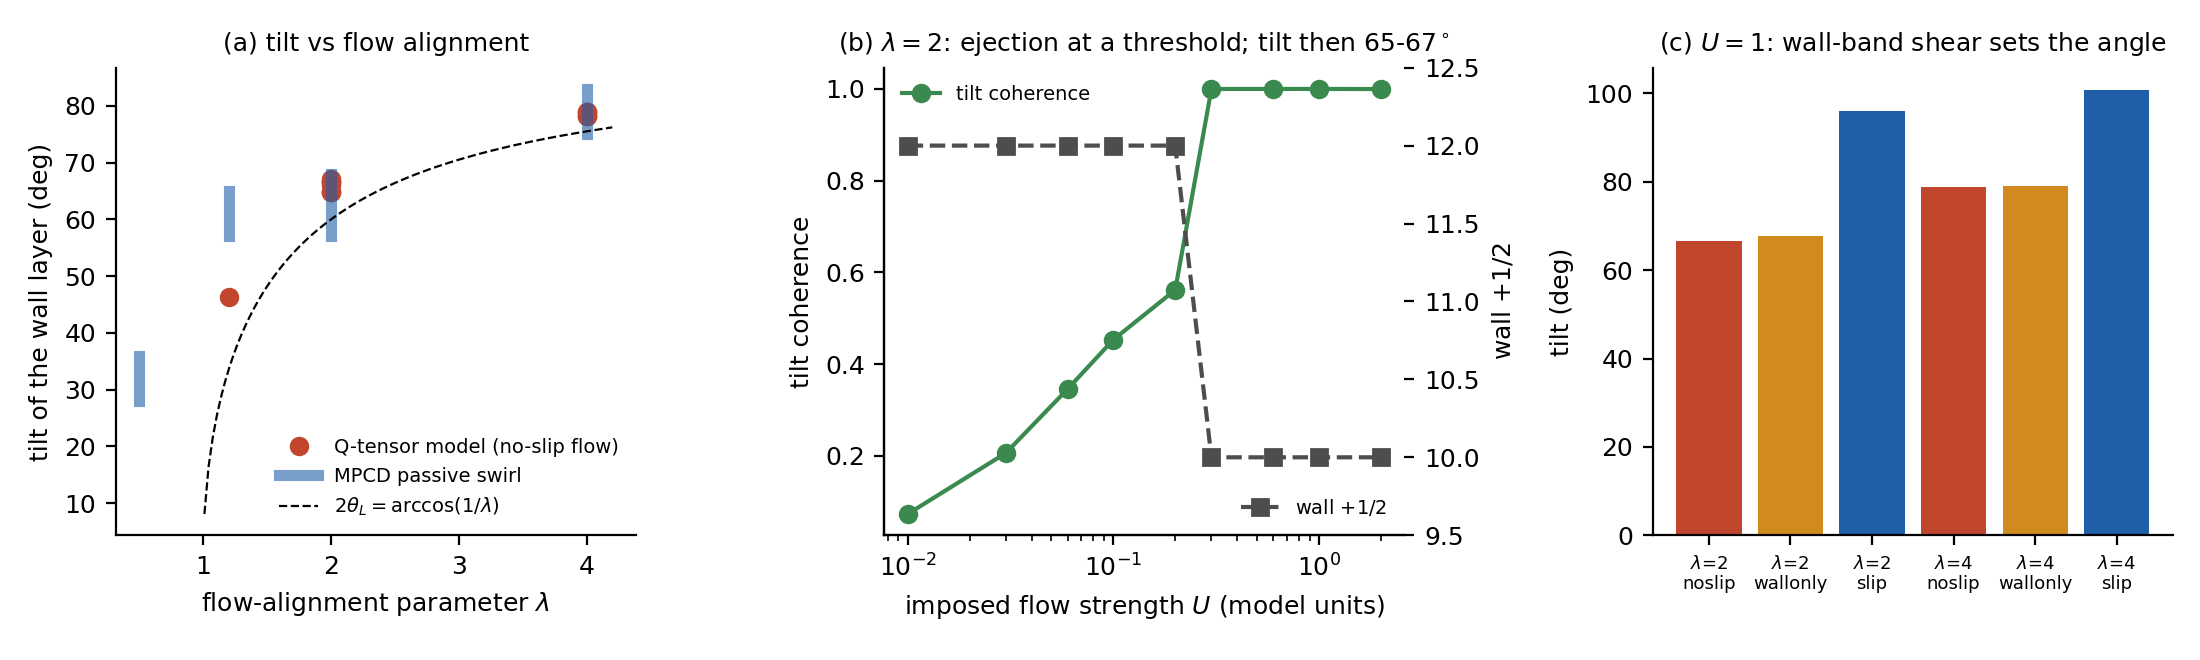
\includegraphics[width=\textwidth]{shear_tilt.png}
\caption{Disk Q-tensor model with the measured no-slip flow (one-way). (a) Tilt after ejection vs $\lambda$: model, MPCD passive swirl, $2\theta_L$. (b) $\lambda=2$: tilt coherence
and wall count vs flow strength (ejection threshold). (c) Tilt with the measured profile, shear only in the wall band, and no shear in the wall band (slip).}\label{fig:sheartilt}
\end{figure}

\subsection{Active continuum model in ellipses; bulk Leslie angle in MPCD (2026-10-10)}\label{sec:contell}
(\texttt{theory/shear\_tilt/ellipse\_active.py}, \texttt{ellipse\_runs/}; \texttt{runs/leslie/}.) The active Q-tensor model with backflow (Sec.~\ref{sec:tiltangle}) in ellipses of the
reference circle's area, arclength-uniform anchoring, $k=6$, $\lambda=2$, noise 0.005, 12\,000 time units: $\varepsilon\le1.2$ circle state at $\zeta=0.3$ and 1 (10 wall, bulk $+1$, coherence 1,
tilt 61--62$^\circ$); $\varepsilon=1.4$ circle state at $\zeta=0.3$, broken at $\zeta=1$; $\varepsilon\ge1.6$ broken (two vortices, coherence 0.48--0.54, circulation 0.18--0.31, wall 9$\to$6,
bulk $+1.5\to+3$). Transition $\varepsilon\approx1.4$--1.6 (MPCD 1.25--1.37), lower at stronger activity (Fig.~\ref{fig:contell}).
Bulk Leslie angle in MPCD (Poiseuille channel, no anchoring): $\lambda=1.2$: 17.4$^\circ$ ($U=5$, $S=0.56$), 14.2$^\circ$ ($U=20$, $S=0.95$), not aligned in half the channel at $U=10$;
$\lambda=1.5$, $U=10$: 22.3$^\circ$; $\lambda=2$, $U=10$: 29.9$^\circ$ (bare 16.8/24.1/30.0$^\circ$; particle-averaged 18.9/14.4/21.5/28.4$^\circ$). Near tumbling the alignment depends on $S$ roughly
as the particle-averaged law; at $\lambda=2$: 32.8/29.9/31.1$^\circ$ ($U=5$/10/20) vs particle-averaged 30.8/28.4/29.2$^\circ$ (offset $+1.8^\circ$). Cavity tilt = twice the measured bulk Leslie angle within $\pm3^\circ$. \emph{Self-propulsion test (continuum, $\zeta=1$):} activity off within 4 cells of the wall: vacancies 0/0/1/2/2.6/4 ($\varepsilon=1$--2.5), as without it; negative winding $k=-6$: 14 wall $-\half$ in circle-like cavities ($=2|k|+2$), 15--16 above the transition, bulk charge $+1.5$--2 in all variants: in the continuum the extra bulk charge comes from bulk activity in elongated cavities, not from self-propelled wall defects and not from the vortex number: with an imposed single vortex, activity only in the wall band or at the cores removes no defects, activity only in the bulk removes two at $\varepsilon=1.6$, 2 (two-vortex fraction 0--0.08). The MPCD wall-band switch-off is not clean (it destroys the circle's single vortex: wall 10$\to$5.5, bulk $+0.8\to+2.5$). The MPCD mirror ($-\half$ hold) stays unexplained.
\begin{figure}[H]\centering
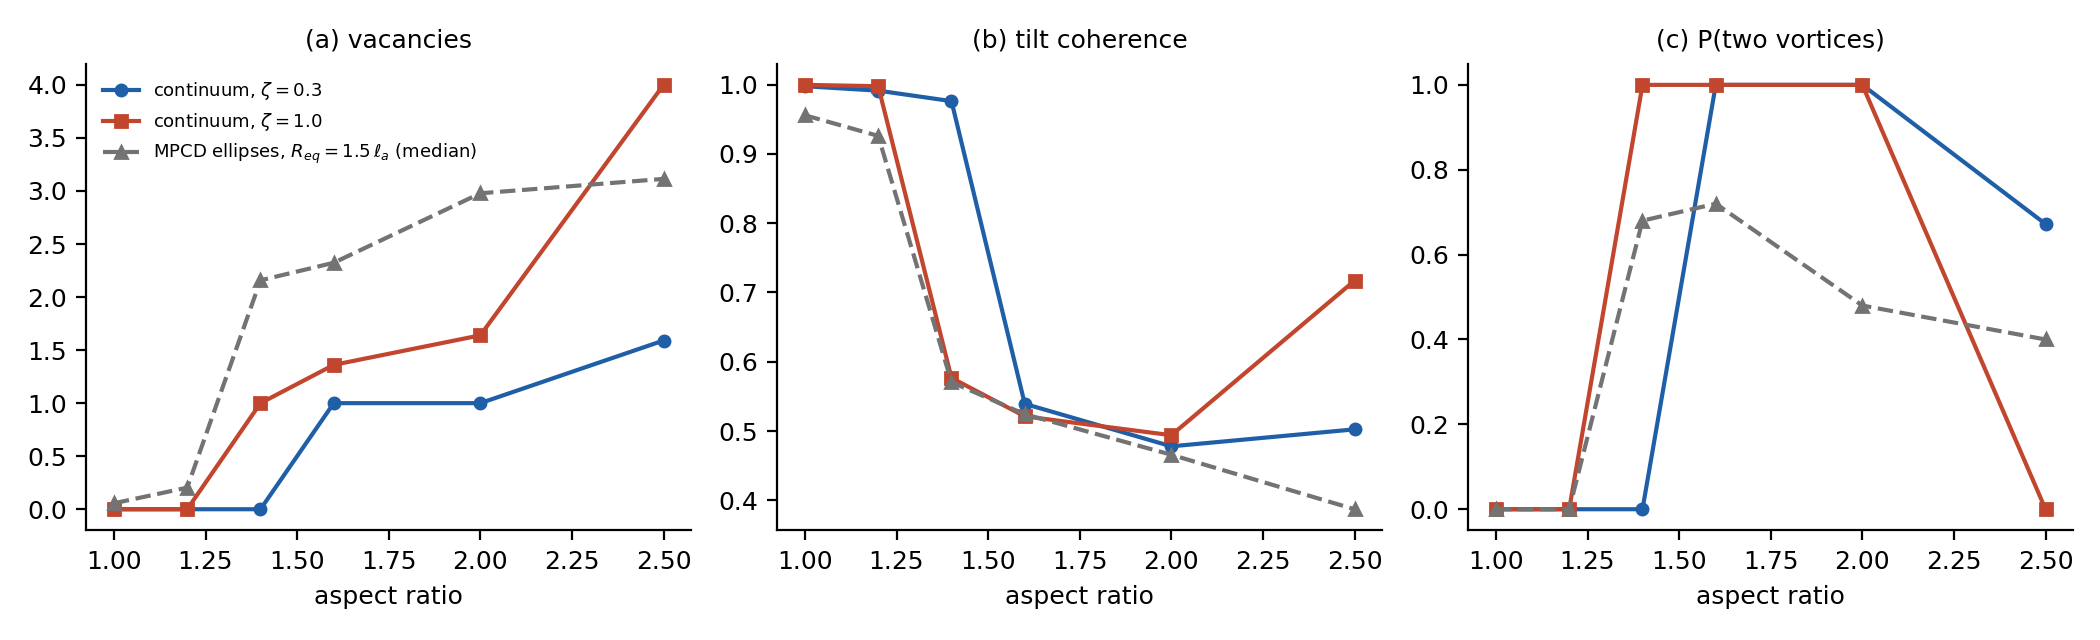
\includegraphics[width=\textwidth]{fig_cont_ellipse.png}
\caption{Active continuum model in ellipses (two activities) against the MPCD ellipse sweep at $R_\mathrm{eq}=1.5\,\la$: (a) vacancies, (b) tilt coherence, (c) fraction of time with two vortices.}\label{fig:contell}
\end{figure}

%=====================================================================
\section{What we know, and what it means}\label{sec:discussion}
\subsection{The picture}
\begin{enumerate}
  \item \textbf{Passive}: the imposed winding produces exactly $2|k|$ defects on fixed sites just inside the wall, at a depth set only by the
        imposed spacing ($\approx0.56+0.094/\rho$ cells), for every shape. Bulk charge 0.
  \item \textbf{Active circles}: two $+\half$ leave the wall and form a bulk of charge $+1$ --- the Euler characteristic of the disc,
        as if the wall had planar anchoring --- while $2k-2$ stay pinned on fixed sites. This holds for $R\approx0.75$--$2\,\la$ at every
        density the anchoring resolves, at every $k$, and is an active effect. The layer and the bulk are almost separate populations:
        wall defects stay $\gg1000$ time units, only 4--10\% of bulk $+\half$ ever dock.
  \item \textbf{The bulk is born with the vortex}: below $R/\la\approx0.4$ all $2k$ $+\half$ sit at the wall and nothing circulates; circulation,
        tilt and the $+1$ bulk appear together at $\approx0.4\,\la$ for every $k$ and $\rho$; at large $R$ the layer becomes less charged
        (bulk $>1$, lattice pinned but under-occupied) as the circulation weakens (Sec.~\ref{sec:onset}).
  \item \textbf{The circular layer is a pinned lattice tilted with the flow}: period $2k-2$, wall $+\half$ leaning 60--65$^\circ$ downstream,
        a single vortex whose circulation collapses on $R/\la$. Layer, pinning and vortex disappear together above $\approx2.5\,\la$.
  \item \textbf{Negative winding}: the wall lattice still has the period of a $+1$ bulk ($2|k|+2$) but is under-occupied, so the bulk is
        positive but below $+1$ until the wall is crowded ($|k|\gtrsim15$). Activity breaks the mirror symmetry.
  \item \textbf{Shape}: at the same size and density, elongation destroys the split. Round shapes (aspect $\lesssim1.2$) behave like
        circles; from aspect $\approx1.4$--1.5 there is no plateau, no pinned lattice and continuous wall--bulk exchange. Ovals and ellipses
        follow the same curve in the aspect ratio, convex or not, and a single lobe-shaped oval behaves like the lobes of a pinched one.
        \textbf{The split is geometric, not fixed by topology.}
  \item \textbf{Everything changes at the same aspect ratio}: charge plateau, lattice pinning, single vortex $\to$ two vortices, escape
        and docking rates (small ovals: aspect 1.17 circle-like, 1.29 intermediate, $\ge1.5$ lost).
  \item \textbf{Crowding pushes back}: a high imposed density ($k$ large at fixed perimeter) refills the wall lattice, stops the upstream
        creep and restores a plateau with a total bulk of $\approx+1$, in ovals as in the mirror runs.
\end{enumerate}
\subsection{Proposed mechanism (to be tested)}
\emph{Elastic part (Sec.~\ref{sec:theory}):} in a circle the wall layer shields the bulk exactly (2D shell theorem with same-sign images), which
explains why the bulk is blind to $k$; the same model predicts the passive layer depth without free parameters (correlation 0.996 over 310 passive
circles) and the screened approach measured in the mirror circles. In an ellipse the passive layer stays evenly spaced and the shielding is imperfect,
but the leftover field is weak ($\lesssim0.06\,\pi K$ inside), so the flow is the more likely driver of the layer loss. Negative winding confirms this (Sec.~\ref{sec:smirror}): the $-\half$ wall layer, whose defects are not self-propelled, survives elongation and the shielding weakens only modestly.\par

In a circle one vortex shears the whole wall in one sense; the tilted wall $+\half$ are held on their sites by the flow and the
anchoring, and the sites are all occupied. In an elongated cavity the flow organises into two vortices (or one that keeps reversing),
which meet along the wall; there the near-wall flow is weak and changes sign, sites empty, and wall defects creep upstream into
vacancies and escape into the bulk, while bulk $+\half$ dock. The charge is then spread through the cavity instead of being stored in a
wall layer. The vacancy--drift correlation (Spearman $-0.82$) and the coincidence of the vortex transition with the charge transition
support this; a direct test is to map vacancies and escapes along the wall relative to the vortex stagnation points.

\subsection{Status of the hypotheses}
\begin{table}[H]\centering\small
\begin{tabularx}{\textwidth}{lXX}\toprule
& Question & Status\\\midrule
H1 & Topological or geometric? & \textbf{Geometric} (Part III); ellipse eMode 0 vs 1 test not needed any more\\
H2 & Does the effect fade at low density ($\rho\la<1$)? & No, down to $\rho\la=0.44$ (Sec.~\ref{sec:ccharge})\\
H3 & Does activity enter only through $\la$? & No; $\zeta=0.07$ is the clean working point (Sec.~\ref{sec:activity})\\
H4 & Does the $+1$ bulk appear with circulation? & \textbf{Supported}: onsets coincide at $R/\la\approx0.4$ for all $k$, $\rho$, both vanish together at large $R$, and the layer is lost where the vortex splits in ovals; causality not tested\\
H5 & Negative winding & Bulk positive, $\to+1$ at $|k|\gtrsim15$; vacancies (Sec.~\ref{sec:mirror}); in ellipses the $-\half$ layer survives elongation (Sec.~\ref{sec:smirror})\\
H6 & Layer formation vs passive layer & Active layer holds $2k-2$, passive $2k$; passive depth law (Sec.~\ref{sec:passive})\\
H7 & Docking at the layer edge & Rates measured (Secs.~\ref{sec:csurv}, \ref{sec:ssurv}); pathway not analysed\\
H8 & Two-lobe cavities: topology vs circulation & Lobes do not act as separate cavities; lobe shape alone loses the layer\\\bottomrule
\end{tabularx}
\end{table}

\subsection{Open items and next runs}
\begin{itemize}
  \item \textbf{Circles to 10 seeds} (running; $+k$ $\approx$ 9--10 Oct, $-k$ $\approx$ 13--14 Oct): refresh every circle figure; check the
        ``less-charged layer'' (Sec.~\ref{sec:sweep}).
  \item \textbf{Oval sweep} (drafted, not launched): 9 shapes $\times$ 3 equivalent sizes $\times$ 4 densities, seed count to decide
        (10 per point would take $\approx4$ days on the server). Open choices: mirror subset, a high-$\rho$ column, ellipses on the server.
  \item Mechanism: vacancies and escapes along the wall vs the vortex stagnation points; near-wall flow and tilt along the arclength in
        ovals; docking pathway (H7).
  \item Fix the ellipse wall distance in \texttt{edge\_criteria.wall()} and \texttt{layer\_depth.py} before quoting $d^*$ or tilt for
        ellipses (Appendix~\ref{app:issues}).
  \item Channel geometry (the infinite-aspect limit) only if a referee asks.
\end{itemize}
\subsection{Candidate split between paper and SI}
\textbf{Main text:} passive vs active circles (maps, $Q(r)$), the layer diagram, the mirror result, the shape result ($Q(c)$, $f^*$
collapse, small-oval crossover), the mechanism figure (pinning, vacancies, drift, one vs two vortices, survival).
\textbf{SI:} resolution limit, $\la$ calibration, compressibility, every edge criterion and their comparison, pair correlations,
activity scan, Fourier details, the $k$ scan, pinch-off and lobe reference, the label tracking. Marked ``SI?'' in the margin above.


\appendix
%=====================================================================
\section{Run inventory}\label{app:runs}
\begin{table}[H]\centering\small
\caption{All run sets ($\zeta=0.07$ unless stated). Paths relative to \texttt{runs/}.}
\begin{tabularx}{\textwidth}{>{\raggedright\arraybackslash}p{4.2cm}X>{\raggedright\arraybackslash}p{2.4cm}}\toprule
set (path) & content & runs, seeds\\\midrule
\texttt{activeLength/L100, L200} & periodic boxes $100^2$, $200^2$; $\zeta=0.05$--0.11 & 9 + 7, 1--2 seeds\\
\texttt{cavityValidation} & passive $R=15$, $k=\pm1\dots\pm5$; active $k=5$, $R=15.9$ & 8\\
\texttt{cavity/resolution\_scan} & resolution limit, passive and active, $R\approx8$--16 & --\\
\texttt{emode2Validation}, \texttt{trackerValidation} & eMode 2 on circle/ellipse; tracker tests & 5 + 7\\
\texttt{cavity/Rscan\_R31.83(\_seeds, \_passive)} & $R=1.43\,\la$, $k=2\dots10$; 10k + 40k & 27 + 9 passive\\
\texttt{cavity/H3pilot(\_seeds), H3high} & activity scan $\zeta=0.05$, 0.06, 0.09, 0.11 at $R=1.43\,\la$ & 4 $\times$ 27\\
\texttt{cavity/density\_check} & $k=8$ at $\zeta=0.07$, 0.09, 0.11 & 3\\
\texttt{cavity/server\_main/main\_act0.07} & main sweep $+k$: $k=1$--20, $\rho=0.03$--0.50; 10k + 100k & 834, 3 seeds\\
\texttt{\dots/main\_act0.07\_neg} & mirror sweep $-k$, $\rho\le0.20$ & 570, 3 seeds\\
\texttt{\dots/main\_passive(\_neg)} & passive references, 10k + 30k & 278 + 190, 1 seed\\
server \texttt{\textasciitilde/Overcharged/runs/cavity} & seeds 4--10 for $\rho\le0.15$, both signs (running since 5 Oct) & 2170\\
\texttt{cassini/T1, T2} & Cassini validation, passive & 6\\
\texttt{cassini/P1--P5, W1--W4} & ovals and ellipses (Table~\ref{tab:ssets}) & 85 active + 12 passive\\\bottomrule
\end{tabularx}
\end{table}
\paragraph{Common parameters.} 2D, mean density 20 particles per cell, $k_BT=1$, $\Delta t=0.1$, collision operator 21 (density-modulated
active dipole), nematic, no-slip walls with phantom particles, homeotropic anchoring (details in Table~\ref{tab:md-params}). Defects every
20 steps (50 in early runs), director and flow fields every 1000 steps. Seeds: runs before 29 Sep (office) and all server runs before
5 Oct were made with a binary that ignored the input seed (independent but not reproducible); later runs are reproducible.

%=====================================================================
\section{Known issues in the code and analysis}\label{app:issues}
Found while writing this document by checking the analysis scripts against the notes (5 Oct). None changes a conclusion stated above;
items 1--2 matter for numbers quoted for ellipses.
\begin{enumerate}
  \item \textbf{Ellipse wall distance:} \texttt{edge\_criteria.wall()} ignores \texttt{aInv}, so \texttt{edge\_criteria}, \texttt{bc\_labels}
        and \texttt{flow\_tilt} treat an ellipse as a circle of radius $R$; \texttt{cassini\_charge}, \texttt{layer\_depth} and
        \texttt{layer\_area} do the same. $f^*$ is unaffected (the ellipse levels are self-similar), $d^*$ and $w_\mathrm{eff}$ are not. No
        ellipse $d^*$ is quoted here. The new scripts of this document use the exact wall polyline.
  \item \textbf{Wall distance $-W/|\nabla W|$} is exact only at the wall: in a circle it gives $(R^2-r^2)/2r$, so a ``6-cell'' cut is
        $\approx5.4$--5.5 cells at $R=31.8$.
  \item \textbf{$d^*$ averaging} is described as arclength-weighted, but the code weights points by $1/|\nabla c|$.
  \item \textbf{Site rule $P_1$} compares raw charges with \texttt{np.isclose}; charges can be up to 0.005 off $\pm\half$, so $P_1$ is biased
        low at the percent level.
  \item \textbf{$q_\mathrm{slow}$} skips occurrences whose track breaks, so the edge count is low and $q_\mathrm{slow}$ high.
  \item \textbf{Speeds} in \texttt{defect\_spatial} use a 3-cell matching radius, which drops fast bulk steps (bulk speeds slightly low;
        same in Sec.~\ref{sec:m-dist}).
  \item \textbf{Tilt window} 0.5 $<|\Delta|<$ 1.8 lost its lower cut in \texttt{criteria\_all}.
  \item \textbf{eMode 1} is not uniform in the ellipse parameter within each period and drops the $O_z$ rotation (no production runs use it).
  \item \textbf{Defaults vs notes:} \texttt{build\_tracks} pairing uses $r_\mathrm{pair}=4$, $t_\mathrm{pair}=2$ (notes say 6 cells, 5 frames);
        the \texttt{defect\_tracks.py} command-line default link radius is 3 (all analyses pass 8); \texttt{wall\_fourier.py} usage line says
        band 3, default 4.
  \item \textbf{Checkpoint restarts} segfault; likely cause: the checkpoint writer prints 31 integers and the reader expects 32 in a
        different order, and \texttt{outFlag.CHCKPNTrcvr} is never initialised. Not used by the run queues (they restart from scratch).
  \item No script reproduces the compressibility numbers (Sec.~\ref{sec:resolution}); they come from an interactive analysis.
\end{enumerate}

\end{document}
